% generated from JIRA project LVV
% using template at <template>.
% Collecting ATM data from folder: "/Data Management/Services/LSP Services|LDM-540"
% using docsteady version 1.2rc10.post1+g1a75e2a
% Please do not edit -- update information in Jira instead

\section{Test Cases Summary}\label{test-cases-summary}

\begin{longtable}[]{p{3cm}p{13cm}}
\toprule
Test Id & Test Name\tabularnewline
\midrule
\endhead
    \hyperref[lvv-t598]{LVV-T598} &
    \href{https://jira.lsstcorp.org/secure/Tests.jspa\#/testCase/LVV-T598}{Verify access to All Released or Authorized Data Products} \tabularnewline
    \hyperref[lvv-t600]{LVV-T600} &
    \href{https://jira.lsstcorp.org/secure/Tests.jspa\#/testCase/LVV-T600}{Verify LSP provides a portal aspect} \tabularnewline
    \hyperref[lvv-t601]{LVV-T601} &
    \href{https://jira.lsstcorp.org/secure/Tests.jspa\#/testCase/LVV-T601}{Verify LSP provides a notebook aspect} \tabularnewline
    \hyperref[lvv-t602]{LVV-T602} &
    \href{https://jira.lsstcorp.org/secure/Tests.jspa\#/testCase/LVV-T602}{Verify LSP provides web API} \tabularnewline
    \hyperref[lvv-t603]{LVV-T603} &
    \href{https://jira.lsstcorp.org/secure/Tests.jspa\#/testCase/LVV-T603}{Verify data access through multiple linked aspects} \tabularnewline
    \hyperref[lvv-t604]{LVV-T604} &
    \href{https://jira.lsstcorp.org/secure/Tests.jspa\#/testCase/LVV-T604}{Verify use of VO standards} \tabularnewline
    \hyperref[lvv-t605]{LVV-T605} &
    \href{https://jira.lsstcorp.org/secure/Tests.jspa\#/testCase/LVV-T605}{Verify that LSP complies with LSST data access policies} \tabularnewline
    \hyperref[lvv-t606]{LVV-T606} &
    \href{https://jira.lsstcorp.org/secure/Tests.jspa\#/testCase/LVV-T606}{Verify semantic linkages between data items} \tabularnewline
    \hyperref[lvv-t607]{LVV-T607} &
    \href{https://jira.lsstcorp.org/secure/Tests.jspa\#/testCase/LVV-T607}{Verify semantic linkages between data items and uncertainties} \tabularnewline
    \hyperref[lvv-t608]{LVV-T608} &
    \href{https://jira.lsstcorp.org/secure/Tests.jspa\#/testCase/LVV-T608}{Verify transfer of Portal data references to Notebook aspect} \tabularnewline
    \hyperref[lvv-t609]{LVV-T609} &
    \href{https://jira.lsstcorp.org/secure/Tests.jspa\#/testCase/LVV-T609}{Verify providing user file storage in LSP} \tabularnewline
    \hyperref[lvv-t610]{LVV-T610} &
    \href{https://jira.lsstcorp.org/secure/Tests.jspa\#/testCase/LVV-T610}{Verify providing user generated database in LSP} \tabularnewline
    \hyperref[lvv-t611]{LVV-T611} &
    \href{https://jira.lsstcorp.org/secure/Tests.jspa\#/testCase/LVV-T611}{Verify access controls in user workspace} \tabularnewline
    \hyperref[lvv-t612]{LVV-T612} &
    \href{https://jira.lsstcorp.org/secure/Tests.jspa\#/testCase/LVV-T612}{Verify ability to download data from LSP} \tabularnewline
    \hyperref[lvv-t613]{LVV-T613} &
    \href{https://jira.lsstcorp.org/secure/Tests.jspa\#/testCase/LVV-T613}{Verify ability to upload data to LSP} \tabularnewline
    \hyperref[lvv-t614]{LVV-T614} &
    \href{https://jira.lsstcorp.org/secure/Tests.jspa\#/testCase/LVV-T614}{Verify ability to transfer data to and from the Workspace} \tabularnewline
    \hyperref[lvv-t615]{LVV-T615} &
    \href{https://jira.lsstcorp.org/secure/Tests.jspa\#/testCase/LVV-T615}{Verify file formats provided for tabular data download} \tabularnewline
    \hyperref[lvv-t616]{LVV-T616} &
    \href{https://jira.lsstcorp.org/secure/Tests.jspa\#/testCase/LVV-T616}{Verify file formats provided for image data download} \tabularnewline
    \hyperref[lvv-t617]{LVV-T617} &
    \href{https://jira.lsstcorp.org/secure/Tests.jspa\#/testCase/LVV-T617}{Verify support for peak volume of moderate-sized queries} \tabularnewline
    \hyperref[lvv-t618]{LVV-T618} &
    \href{https://jira.lsstcorp.org/secure/Tests.jspa\#/testCase/LVV-T618}{Verify support for peak volume of queries on all Objects} \tabularnewline
    \hyperref[lvv-t619]{LVV-T619} &
    \href{https://jira.lsstcorp.org/secure/Tests.jspa\#/testCase/LVV-T619}{Verify LSP handles peak volume of queries} \tabularnewline
    \hyperref[lvv-t620]{LVV-T620} &
    \href{https://jira.lsstcorp.org/secure/Tests.jspa\#/testCase/LVV-T620}{Verify LSP supports required download bandwidth} \tabularnewline
    \hyperref[lvv-t621]{LVV-T621} &
    \href{https://jira.lsstcorp.org/secure/Tests.jspa\#/testCase/LVV-T621}{Verify LSP user reference and documentation} \tabularnewline
    \hyperref[lvv-t622]{LVV-T622} &
    \href{https://jira.lsstcorp.org/secure/Tests.jspa\#/testCase/LVV-T622}{Verify LSP only available to authenticated users} \tabularnewline
    \hyperref[lvv-t623]{LVV-T623} &
    \href{https://jira.lsstcorp.org/secure/Tests.jspa\#/testCase/LVV-T623}{Verify support for new LSP users} \tabularnewline
    \hyperref[lvv-t624]{LVV-T624} &
    \href{https://jira.lsstcorp.org/secure/Tests.jspa\#/testCase/LVV-T624}{Verify implementation of common identity across LSP aspects} \tabularnewline
    \hyperref[lvv-t625]{LVV-T625} &
    \href{https://jira.lsstcorp.org/secure/Tests.jspa\#/testCase/LVV-T625}{Verify authentication via external identity providers} \tabularnewline
    \hyperref[lvv-t626]{LVV-T626} &
    \href{https://jira.lsstcorp.org/secure/Tests.jspa\#/testCase/LVV-T626}{Verify LSP identity can have multiple associated credentials} \tabularnewline
    \hyperref[lvv-t627]{LVV-T627} &
    \href{https://jira.lsstcorp.org/secure/Tests.jspa\#/testCase/LVV-T627}{Verify implementation of Acceptable Use Policy} \tabularnewline
    \hyperref[lvv-t628]{LVV-T628} &
    \href{https://jira.lsstcorp.org/secure/Tests.jspa\#/testCase/LVV-T628}{Verify LSP connections encrypted} \tabularnewline
    \hyperref[lvv-t629]{LVV-T629} &
    \href{https://jira.lsstcorp.org/secure/Tests.jspa\#/testCase/LVV-T629}{Verify privacy of users' activities} \tabularnewline
    \hyperref[lvv-t630]{LVV-T630} &
    \href{https://jira.lsstcorp.org/secure/Tests.jspa\#/testCase/LVV-T630}{Verify multiple LSP instances} \tabularnewline
    \hyperref[lvv-t631]{LVV-T631} &
    \href{https://jira.lsstcorp.org/secure/Tests.jspa\#/testCase/LVV-T631}{Verify LSP access from the public Internet (IPv4)} \tabularnewline
    \hyperref[lvv-t632]{LVV-T632} &
    \href{https://jira.lsstcorp.org/secure/Tests.jspa\#/testCase/LVV-T632}{Verify LSP access from the public Internet (IPv6)} \tabularnewline
    \hyperref[lvv-t633]{LVV-T633} &
    \href{https://jira.lsstcorp.org/secure/Tests.jspa\#/testCase/LVV-T633}{Verify indication of system availability} \tabularnewline
    \hyperref[lvv-t634]{LVV-T634} &
    \href{https://jira.lsstcorp.org/secure/Tests.jspa\#/testCase/LVV-T634}{Verify Portal is a web application} \tabularnewline
    \hyperref[lvv-t635]{LVV-T635} &
    \href{https://jira.lsstcorp.org/secure/Tests.jspa\#/testCase/LVV-T635}{Verify Portal discovery of all data products} \tabularnewline
    \hyperref[lvv-t636]{LVV-T636} &
    \href{https://jira.lsstcorp.org/secure/Tests.jspa\#/testCase/LVV-T636}{Verify Portal access to Workspace} \tabularnewline
    \hyperref[lvv-t637]{LVV-T637} &
    \href{https://jira.lsstcorp.org/secure/Tests.jspa\#/testCase/LVV-T637}{Verify Portal provides semantic linkages between data products} \tabularnewline
    \hyperref[lvv-t638]{LVV-T638} &
    \href{https://jira.lsstcorp.org/secure/Tests.jspa\#/testCase/LVV-T638}{Verify access to calibration products via Portal} \tabularnewline
    \hyperref[lvv-t639]{LVV-T639} &
    \href{https://jira.lsstcorp.org/secure/Tests.jspa\#/testCase/LVV-T639}{Verify associations between single images and coadds} \tabularnewline
    \hyperref[lvv-t640]{LVV-T640} &
    \href{https://jira.lsstcorp.org/secure/Tests.jspa\#/testCase/LVV-T640}{Verify access to external archives from Portal} \tabularnewline
    \hyperref[lvv-t641]{LVV-T641} &
    \href{https://jira.lsstcorp.org/secure/Tests.jspa\#/testCase/LVV-T641}{Verify API for Access to Portal Session State} \tabularnewline
    \hyperref[lvv-t642]{LVV-T642} &
    \href{https://jira.lsstcorp.org/secure/Tests.jspa\#/testCase/LVV-T642}{Verify Portal supports both synchronous and asynchronous queries} \tabularnewline
    \hyperref[lvv-t643]{LVV-T643} &
    \href{https://jira.lsstcorp.org/secure/Tests.jspa\#/testCase/LVV-T643}{Verify capability to run long queries in the background} \tabularnewline
    \hyperref[lvv-t644]{LVV-T644} &
    \href{https://jira.lsstcorp.org/secure/Tests.jspa\#/testCase/LVV-T644}{Verify user notification of query status} \tabularnewline
    \hyperref[lvv-t645]{LVV-T645} &
    \href{https://jira.lsstcorp.org/secure/Tests.jspa\#/testCase/LVV-T645}{Verify limitation of query results size} \tabularnewline
    \hyperref[lvv-t646]{LVV-T646} &
    \href{https://jira.lsstcorp.org/secure/Tests.jspa\#/testCase/LVV-T646}{Verify ability to browse query history} \tabularnewline
    \hyperref[lvv-t647]{LVV-T647} &
    \href{https://jira.lsstcorp.org/secure/Tests.jspa\#/testCase/LVV-T647}{Verify implementation of saving of queries} \tabularnewline
    \hyperref[lvv-t648]{LVV-T648} &
    \href{https://jira.lsstcorp.org/secure/Tests.jspa\#/testCase/LVV-T648}{Verify implementation of generic queries in API aspect} \tabularnewline
    \hyperref[lvv-t649]{LVV-T649} &
    \href{https://jira.lsstcorp.org/secure/Tests.jspa\#/testCase/LVV-T649}{Verify implementation of form-based generic query in API aspect} \tabularnewline
    \hyperref[lvv-t650]{LVV-T650} &
    \href{https://jira.lsstcorp.org/secure/Tests.jspa\#/testCase/LVV-T650}{Verify implementation of ADQL-based generic query in API aspect} \tabularnewline
    \hyperref[lvv-t651]{LVV-T651} &
    \href{https://jira.lsstcorp.org/secure/Tests.jspa\#/testCase/LVV-T651}{Verify estimation of query result size} \tabularnewline
    \hyperref[lvv-t652]{LVV-T652} &
    \href{https://jira.lsstcorp.org/secure/Tests.jspa\#/testCase/LVV-T652}{Verify query by unique identifier} \tabularnewline
    \hyperref[lvv-t653]{LVV-T653} &
    \href{https://jira.lsstcorp.org/secure/Tests.jspa\#/testCase/LVV-T653}{Verify query by object or source identifier} \tabularnewline
    \hyperref[lvv-t654]{LVV-T654} &
    \href{https://jira.lsstcorp.org/secure/Tests.jspa\#/testCase/LVV-T654}{Verify query by Solar System object identifier} \tabularnewline
    \hyperref[lvv-t655]{LVV-T655} &
    \href{https://jira.lsstcorp.org/secure/Tests.jspa\#/testCase/LVV-T655}{Verify query by position on the sky} \tabularnewline
    \hyperref[lvv-t656]{LVV-T656} &
    \href{https://jira.lsstcorp.org/secure/Tests.jspa\#/testCase/LVV-T656}{Verify query by list of positions} \tabularnewline
    \hyperref[lvv-t657]{LVV-T657} &
    \href{https://jira.lsstcorp.org/secure/Tests.jspa\#/testCase/LVV-T657}{Verify implementation of astrophysical coordinate systems} \tabularnewline
    \hyperref[lvv-t658]{LVV-T658} &
    \href{https://jira.lsstcorp.org/secure/Tests.jspa\#/testCase/LVV-T658}{Verify positional query by astrophysical source name} \tabularnewline
    \hyperref[lvv-t659]{LVV-T659} &
    \href{https://jira.lsstcorp.org/secure/Tests.jspa\#/testCase/LVV-T659}{Verify positional query by Source or Object name} \tabularnewline
    \hyperref[lvv-t660]{LVV-T660} &
    \href{https://jira.lsstcorp.org/secure/Tests.jspa\#/testCase/LVV-T660}{Verify positional query based on Solar System object names} \tabularnewline
    \hyperref[lvv-t661]{LVV-T661} &
    \href{https://jira.lsstcorp.org/secure/Tests.jspa\#/testCase/LVV-T661}{Verify query by cone search} \tabularnewline
    \hyperref[lvv-t662]{LVV-T662} &
    \href{https://jira.lsstcorp.org/secure/Tests.jspa\#/testCase/LVV-T662}{Verify query by box search} \tabularnewline
    \hyperref[lvv-t663]{LVV-T663} &
    \href{https://jira.lsstcorp.org/secure/Tests.jspa\#/testCase/LVV-T663}{Verify query by time of observation} \tabularnewline
    \hyperref[lvv-t664]{LVV-T664} &
    \href{https://jira.lsstcorp.org/secure/Tests.jspa\#/testCase/LVV-T664}{Verify implementation of user-friendly tabular query} \tabularnewline
    \hyperref[lvv-t666]{LVV-T666} &
    \href{https://jira.lsstcorp.org/secure/Tests.jspa\#/testCase/LVV-T666}{Verify query by image metadata} \tabularnewline
    \hyperref[lvv-t667]{LVV-T667} &
    \href{https://jira.lsstcorp.org/secure/Tests.jspa\#/testCase/LVV-T667}{Verify queries on the alerts database} \tabularnewline
    \hyperref[lvv-t668]{LVV-T668} &
    \href{https://jira.lsstcorp.org/secure/Tests.jspa\#/testCase/LVV-T668}{Verify access to original alert state} \tabularnewline
    \hyperref[lvv-t669]{LVV-T669} &
    \href{https://jira.lsstcorp.org/secure/Tests.jspa\#/testCase/LVV-T669}{Verify query for single-epoch visit images} \tabularnewline
    \hyperref[lvv-t670]{LVV-T670} &
    \href{https://jira.lsstcorp.org/secure/Tests.jspa\#/testCase/LVV-T670}{Verify query for single-epoch raft images} \tabularnewline
    \hyperref[lvv-t671]{LVV-T671} &
    \href{https://jira.lsstcorp.org/secure/Tests.jspa\#/testCase/LVV-T671}{Verify query for single-epoch CCD images} \tabularnewline
    \hyperref[lvv-t672]{LVV-T672} &
    \href{https://jira.lsstcorp.org/secure/Tests.jspa\#/testCase/LVV-T672}{Verify metadata query for single-epoch images} \tabularnewline
    \hyperref[lvv-t673]{LVV-T673} &
    \href{https://jira.lsstcorp.org/secure/Tests.jspa\#/testCase/LVV-T673}{Verify query for coadds by image metadata} \tabularnewline
    \hyperref[lvv-t674]{LVV-T674} &
    \href{https://jira.lsstcorp.org/secure/Tests.jspa\#/testCase/LVV-T674}{Verify query for coadd image cutouts} \tabularnewline
    \hyperref[lvv-t675]{LVV-T675} &
    \href{https://jira.lsstcorp.org/secure/Tests.jspa\#/testCase/LVV-T675}{Verify query for single-epoch image cutouts} \tabularnewline
    \hyperref[lvv-t676]{LVV-T676} &
    \href{https://jira.lsstcorp.org/secure/Tests.jspa\#/testCase/LVV-T676}{Verify display of native single-visit images} \tabularnewline
    \hyperref[lvv-t677]{LVV-T677} &
    \href{https://jira.lsstcorp.org/secure/Tests.jspa\#/testCase/LVV-T677}{Verify Portal provides visualization of tabular and image data} \tabularnewline
    \hyperref[lvv-t678]{LVV-T678} &
    \href{https://jira.lsstcorp.org/secure/Tests.jspa\#/testCase/LVV-T678}{Verify visualization of ancillary information} \tabularnewline
    \hyperref[lvv-t679]{LVV-T679} &
    \href{https://jira.lsstcorp.org/secure/Tests.jspa\#/testCase/LVV-T679}{Verify visualization linking image and tabular data} \tabularnewline
    \hyperref[lvv-t680]{LVV-T680} &
    \href{https://jira.lsstcorp.org/secure/Tests.jspa\#/testCase/LVV-T680}{Verify visualization tool for uploaded tabular or image data} \tabularnewline
    \hyperref[lvv-t681]{LVV-T681} &
    \href{https://jira.lsstcorp.org/secure/Tests.jspa\#/testCase/LVV-T681}{Verify visualization of workspace data} \tabularnewline
    \hyperref[lvv-t682]{LVV-T682} &
    \href{https://jira.lsstcorp.org/secure/Tests.jspa\#/testCase/LVV-T682}{Verify availability of property sheets for table rows} \tabularnewline
    \hyperref[lvv-t683]{LVV-T683} &
    \href{https://jira.lsstcorp.org/secure/Tests.jspa\#/testCase/LVV-T683}{Verify visualization of alerts} \tabularnewline
    \hyperref[lvv-t684]{LVV-T684} &
    \href{https://jira.lsstcorp.org/secure/Tests.jspa\#/testCase/LVV-T684}{Verify display of tabular data} \tabularnewline
    \hyperref[lvv-t685]{LVV-T685} &
    \href{https://jira.lsstcorp.org/secure/Tests.jspa\#/testCase/LVV-T685}{Verify column selection from tables} \tabularnewline
    \hyperref[lvv-t686]{LVV-T686} &
    \href{https://jira.lsstcorp.org/secure/Tests.jspa\#/testCase/LVV-T686}{Verify capability to re-order columns in displayed tabular data} \tabularnewline
    \hyperref[lvv-t687]{LVV-T687} &
    \href{https://jira.lsstcorp.org/secure/Tests.jspa\#/testCase/LVV-T687}{Verify capability of copying data in tables} \tabularnewline
    \hyperref[lvv-t688]{LVV-T688} &
    \href{https://jira.lsstcorp.org/secure/Tests.jspa\#/testCase/LVV-T688}{Verify row selection from tables} \tabularnewline
    \hyperref[lvv-t689]{LVV-T689} &
    \href{https://jira.lsstcorp.org/secure/Tests.jspa\#/testCase/LVV-T689}{Verify capability to display tabular data in paged format} \tabularnewline
    \hyperref[lvv-t690]{LVV-T690} &
    \href{https://jira.lsstcorp.org/secure/Tests.jspa\#/testCase/LVV-T690}{Verify creation and display of X-Y scatter plots} \tabularnewline
    \hyperref[lvv-t691]{LVV-T691} &
    \href{https://jira.lsstcorp.org/secure/Tests.jspa\#/testCase/LVV-T691}{Verify creation and display of histogram plots} \tabularnewline
    \hyperref[lvv-t692]{LVV-T692} &
    \href{https://jira.lsstcorp.org/secure/Tests.jspa\#/testCase/LVV-T692}{Verify capability to change symbol shapes, sizes, and colors in XY(Z)
scatter plots} \tabularnewline
    \hyperref[lvv-t693]{LVV-T693} &
    \href{https://jira.lsstcorp.org/secure/Tests.jspa\#/testCase/LVV-T693}{Verify visualization of uncertainties in plots} \tabularnewline
    \hyperref[lvv-t694]{LVV-T694} &
    \href{https://jira.lsstcorp.org/secure/Tests.jspa\#/testCase/LVV-T694}{Verify visualization of asymmetric uncertainties} \tabularnewline
    \hyperref[lvv-t695]{LVV-T695} &
    \href{https://jira.lsstcorp.org/secure/Tests.jspa\#/testCase/LVV-T695}{Verify visualization of upper and lower limits in plots} \tabularnewline
    \hyperref[lvv-t696]{LVV-T696} &
    \href{https://jira.lsstcorp.org/secure/Tests.jspa\#/testCase/LVV-T696}{Verify visualization of multiple XY plots on the same display} \tabularnewline
    \hyperref[lvv-t697]{LVV-T697} &
    \href{https://jira.lsstcorp.org/secure/Tests.jspa\#/testCase/LVV-T697}{Verify display of raft and full focal-plane single-visit images} \tabularnewline
    \hyperref[lvv-t698]{LVV-T698} &
    \href{https://jira.lsstcorp.org/secure/Tests.jspa\#/testCase/LVV-T698}{Verify display of cutout from single-visit image} \tabularnewline
    \hyperref[lvv-t699]{LVV-T699} &
    \href{https://jira.lsstcorp.org/secure/Tests.jspa\#/testCase/LVV-T699}{Verify display of native coadd images} \tabularnewline
    \hyperref[lvv-t700]{LVV-T700} &
    \href{https://jira.lsstcorp.org/secure/Tests.jspa\#/testCase/LVV-T700}{Verify display of coadd cutouts and mosaics} \tabularnewline
    \hyperref[lvv-t701]{LVV-T701} &
    \href{https://jira.lsstcorp.org/secure/Tests.jspa\#/testCase/LVV-T701}{Verify display of calibration images} \tabularnewline
    \hyperref[lvv-t702]{LVV-T702} &
    \href{https://jira.lsstcorp.org/secure/Tests.jspa\#/testCase/LVV-T702}{Verify display of user-provided images} \tabularnewline
    \hyperref[lvv-t703]{LVV-T703} &
    \href{https://jira.lsstcorp.org/secure/Tests.jspa\#/testCase/LVV-T703}{Verify display of image property sheet} \tabularnewline
    \hyperref[lvv-t704]{LVV-T704} &
    \href{https://jira.lsstcorp.org/secure/Tests.jspa\#/testCase/LVV-T704}{Verify that coordinate display tools are provided for images} \tabularnewline
    \hyperref[lvv-t705]{LVV-T705} &
    \href{https://jira.lsstcorp.org/secure/Tests.jspa\#/testCase/LVV-T705}{Verify image pixel content display} \tabularnewline
    \hyperref[lvv-t706]{LVV-T706} &
    \href{https://jira.lsstcorp.org/secure/Tests.jspa\#/testCase/LVV-T706}{Verify spatial manipulation of images} \tabularnewline
    \hyperref[lvv-t707]{LVV-T707} &
    \href{https://jira.lsstcorp.org/secure/Tests.jspa\#/testCase/LVV-T707}{Verify multi-image scaling and alignment} \tabularnewline
    \hyperref[lvv-t708]{LVV-T708} &
    \href{https://jira.lsstcorp.org/secure/Tests.jspa\#/testCase/LVV-T708}{Verify manipulation of image appearance} \tabularnewline
    \hyperref[lvv-t709]{LVV-T709} &
    \href{https://jira.lsstcorp.org/secure/Tests.jspa\#/testCase/LVV-T709}{Verify display of image mask and variance overlays} \tabularnewline
    \hyperref[lvv-t710]{LVV-T710} &
    \href{https://jira.lsstcorp.org/secure/Tests.jspa\#/testCase/LVV-T710}{Verify display of plot overlays on images} \tabularnewline
    \hyperref[lvv-t711]{LVV-T711} &
    \href{https://jira.lsstcorp.org/secure/Tests.jspa\#/testCase/LVV-T711}{Verify capability to adjust the appearance of plot overlays on images} \tabularnewline
    \hyperref[lvv-t712]{LVV-T712} &
    \href{https://jira.lsstcorp.org/secure/Tests.jspa\#/testCase/LVV-T712}{Verify display all-sky HEALPix image} \tabularnewline
    \hyperref[lvv-t713]{LVV-T713} &
    \href{https://jira.lsstcorp.org/secure/Tests.jspa\#/testCase/LVV-T713}{Verify ability to zoom in/out on a HEALPix image} \tabularnewline
    \hyperref[lvv-t714]{LVV-T714} &
    \href{https://jira.lsstcorp.org/secure/Tests.jspa\#/testCase/LVV-T714}{Verify panning in HEALPix image display} \tabularnewline
    \hyperref[lvv-t715]{LVV-T715} &
    \href{https://jira.lsstcorp.org/secure/Tests.jspa\#/testCase/LVV-T715}{Verify selection of HEALPix pixels} \tabularnewline
    \hyperref[lvv-t716]{LVV-T716} &
    \href{https://jira.lsstcorp.org/secure/Tests.jspa\#/testCase/LVV-T716}{Verify retrieval of HEALPix-associated data} \tabularnewline
    \hyperref[lvv-t717]{LVV-T717} &
    \href{https://jira.lsstcorp.org/secure/Tests.jspa\#/testCase/LVV-T717}{Verify broad applicability of coordinate display} \tabularnewline
    \hyperref[lvv-t718]{LVV-T718} &
    \href{https://jira.lsstcorp.org/secure/Tests.jspa\#/testCase/LVV-T718}{Verify point coordinate display} \tabularnewline
    \hyperref[lvv-t719]{LVV-T719} &
    \href{https://jira.lsstcorp.org/secure/Tests.jspa\#/testCase/LVV-T719}{Verify distance measurement tool} \tabularnewline
    \hyperref[lvv-t720]{LVV-T720} &
    \href{https://jira.lsstcorp.org/secure/Tests.jspa\#/testCase/LVV-T720}{Verify coordinate grid overlays} \tabularnewline
    \hyperref[lvv-t721]{LVV-T721} &
    \href{https://jira.lsstcorp.org/secure/Tests.jspa\#/testCase/LVV-T721}{Verify astrophysical compass overlay} \tabularnewline
    \hyperref[lvv-t722]{LVV-T722} &
    \href{https://jira.lsstcorp.org/secure/Tests.jspa\#/testCase/LVV-T722}{Verify geometric figure overlays} \tabularnewline
    \hyperref[lvv-t723]{LVV-T723} &
    \href{https://jira.lsstcorp.org/secure/Tests.jspa\#/testCase/LVV-T723}{Verify sorting of tabular data by column} \tabularnewline
    \hyperref[lvv-t724]{LVV-T724} &
    \href{https://jira.lsstcorp.org/secure/Tests.jspa\#/testCase/LVV-T724}{Verify simple filtering of tabular data} \tabularnewline
    \hyperref[lvv-t725]{LVV-T725} &
    \href{https://jira.lsstcorp.org/secure/Tests.jspa\#/testCase/LVV-T725}{Verify calculated filtering of tabular data} \tabularnewline
    \hyperref[lvv-t726]{LVV-T726} &
    \href{https://jira.lsstcorp.org/secure/Tests.jspa\#/testCase/LVV-T726}{Verify filtering data by multiple table columns} \tabularnewline
    \hyperref[lvv-t727]{LVV-T727} &
    \href{https://jira.lsstcorp.org/secure/Tests.jspa\#/testCase/LVV-T727}{Verify calculated tabular data columns} \tabularnewline
    \hyperref[lvv-t728]{LVV-T728} &
    \href{https://jira.lsstcorp.org/secure/Tests.jspa\#/testCase/LVV-T728}{Verify statistical measurements on tabular data} \tabularnewline
    \hyperref[lvv-t729]{LVV-T729} &
    \href{https://jira.lsstcorp.org/secure/Tests.jspa\#/testCase/LVV-T729}{Verify saving of displayed tabular data} \tabularnewline
    \hyperref[lvv-t730]{LVV-T730} &
    \href{https://jira.lsstcorp.org/secure/Tests.jspa\#/testCase/LVV-T730}{Verify creation and display of false-color images} \tabularnewline
    \hyperref[lvv-t731]{LVV-T731} &
    \href{https://jira.lsstcorp.org/secure/Tests.jspa\#/testCase/LVV-T731}{Verify statistical measurements on user-selected regions of images} \tabularnewline
    \hyperref[lvv-t732]{LVV-T732} &
    \href{https://jira.lsstcorp.org/secure/Tests.jspa\#/testCase/LVV-T732}{Verify overlay of catalog sources/objects on images} \tabularnewline
    \hyperref[lvv-t733]{LVV-T733} &
    \href{https://jira.lsstcorp.org/secure/Tests.jspa\#/testCase/LVV-T733}{Verify overlay of LSST-derived orbits on images} \tabularnewline
    \hyperref[lvv-t734]{LVV-T734} &
    \href{https://jira.lsstcorp.org/secure/Tests.jspa\#/testCase/LVV-T734}{Verify overlay of user-supplied catalogs on images} \tabularnewline
    \hyperref[lvv-t735]{LVV-T735} &
    \href{https://jira.lsstcorp.org/secure/Tests.jspa\#/testCase/LVV-T735}{Verify overlay of user-supplied region files on images} \tabularnewline
    \hyperref[lvv-t736]{LVV-T736} &
    \href{https://jira.lsstcorp.org/secure/Tests.jspa\#/testCase/LVV-T736}{Verify overlay of camera artifacts on images} \tabularnewline
    \hyperref[lvv-t737]{LVV-T737} &
    \href{https://jira.lsstcorp.org/secure/Tests.jspa\#/testCase/LVV-T737}{Verify single-object time-domain image view} \tabularnewline
    \hyperref[lvv-t738]{LVV-T738} &
    \href{https://jira.lsstcorp.org/secure/Tests.jspa\#/testCase/LVV-T738}{Verify position-based time-domain image view} \tabularnewline
    \hyperref[lvv-t739]{LVV-T739} &
    \href{https://jira.lsstcorp.org/secure/Tests.jspa\#/testCase/LVV-T739}{Verify display of light curves} \tabularnewline
    \hyperref[lvv-t740]{LVV-T740} &
    \href{https://jira.lsstcorp.org/secure/Tests.jspa\#/testCase/LVV-T740}{Verify linked tables, plots, and images} \tabularnewline
    \hyperref[lvv-t741]{LVV-T741} &
    \href{https://jira.lsstcorp.org/secure/Tests.jspa\#/testCase/LVV-T741}{Verify capability to select data from a plot or image} \tabularnewline
    \hyperref[lvv-t742]{LVV-T742} &
    \href{https://jira.lsstcorp.org/secure/Tests.jspa\#/testCase/LVV-T742}{Verify saving data selection from a plot or image} \tabularnewline
    \hyperref[lvv-t743]{LVV-T743} &
    \href{https://jira.lsstcorp.org/secure/Tests.jspa\#/testCase/LVV-T743}{Verify access to user databases} \tabularnewline
    \hyperref[lvv-t744]{LVV-T744} &
    \href{https://jira.lsstcorp.org/secure/Tests.jspa\#/testCase/LVV-T744}{Verify tabular data download} \tabularnewline
    \hyperref[lvv-t745]{LVV-T745} &
    \href{https://jira.lsstcorp.org/secure/Tests.jspa\#/testCase/LVV-T745}{Verify image data download} \tabularnewline
    \hyperref[lvv-t746]{LVV-T746} &
    \href{https://jira.lsstcorp.org/secure/Tests.jspa\#/testCase/LVV-T746}{Verify selected image download} \tabularnewline
    \hyperref[lvv-t747]{LVV-T747} &
    \href{https://jira.lsstcorp.org/secure/Tests.jspa\#/testCase/LVV-T747}{Verify estimation of data download volume} \tabularnewline
    \hyperref[lvv-t748]{LVV-T748} &
    \href{https://jira.lsstcorp.org/secure/Tests.jspa\#/testCase/LVV-T748}{Verify notification of long download completion} \tabularnewline
    \hyperref[lvv-t749]{LVV-T749} &
    \href{https://jira.lsstcorp.org/secure/Tests.jspa\#/testCase/LVV-T749}{Verify API for visualization components} \tabularnewline
    \hyperref[lvv-t750]{LVV-T750} &
    \href{https://jira.lsstcorp.org/secure/Tests.jspa\#/testCase/LVV-T750}{Verify implementation of storage quotas status} \tabularnewline
    \hyperref[lvv-t751]{LVV-T751} &
    \href{https://jira.lsstcorp.org/secure/Tests.jspa\#/testCase/LVV-T751}{Verify implementation of computational quotas status} \tabularnewline
    \hyperref[lvv-t752]{LVV-T752} &
    \href{https://jira.lsstcorp.org/secure/Tests.jspa\#/testCase/LVV-T752}{Verify saved Portal display preferences} \tabularnewline
    \hyperref[lvv-t753]{LVV-T753} &
    \href{https://jira.lsstcorp.org/secure/Tests.jspa\#/testCase/LVV-T753}{Verify alert subscription service} \tabularnewline
    \hyperref[lvv-t754]{LVV-T754} &
    \href{https://jira.lsstcorp.org/secure/Tests.jspa\#/testCase/LVV-T754}{Verify availability of pre-defined alert filters} \tabularnewline
    \hyperref[lvv-t755]{LVV-T755} &
    \href{https://jira.lsstcorp.org/secure/Tests.jspa\#/testCase/LVV-T755}{Verify availability of user-defined alert filters} \tabularnewline
    \hyperref[lvv-t756]{LVV-T756} &
    \href{https://jira.lsstcorp.org/secure/Tests.jspa\#/testCase/LVV-T756}{Verify monitoring of alert subscription} \tabularnewline
    \hyperref[lvv-t757]{LVV-T757} &
    \href{https://jira.lsstcorp.org/secure/Tests.jspa\#/testCase/LVV-T757}{Verify access to survey documentation} \tabularnewline
    \hyperref[lvv-t758]{LVV-T758} &
    \href{https://jira.lsstcorp.org/secure/Tests.jspa\#/testCase/LVV-T758}{Verify access to Portal documentation} \tabularnewline
    \hyperref[lvv-t759]{LVV-T759} &
    \href{https://jira.lsstcorp.org/secure/Tests.jspa\#/testCase/LVV-T759}{Verify access to Portal API documentation} \tabularnewline
    \hyperref[lvv-t760]{LVV-T760} &
    \href{https://jira.lsstcorp.org/secure/Tests.jspa\#/testCase/LVV-T760}{Verify tolerance of database changes} \tabularnewline
    \hyperref[lvv-t761]{LVV-T761} &
    \href{https://jira.lsstcorp.org/secure/Tests.jspa\#/testCase/LVV-T761}{Verify implementation of system-busy notification} \tabularnewline
    \hyperref[lvv-t762]{LVV-T762} &
    \href{https://jira.lsstcorp.org/secure/Tests.jspa\#/testCase/LVV-T762}{Verify availability of interactive Python environment} \tabularnewline
    \hyperref[lvv-t763]{LVV-T763} &
    \href{https://jira.lsstcorp.org/secure/Tests.jspa\#/testCase/LVV-T763}{Verify availability of Unix shell access} \tabularnewline
    \hyperref[lvv-t764]{LVV-T764} &
    \href{https://jira.lsstcorp.org/secure/Tests.jspa\#/testCase/LVV-T764}{Verify availability of containerized software releases} \tabularnewline
    \hyperref[lvv-t765]{LVV-T765} &
    \href{https://jira.lsstcorp.org/secure/Tests.jspa\#/testCase/LVV-T765}{Verify latency of release deployment} \tabularnewline
    \hyperref[lvv-t766]{LVV-T766} &
    \href{https://jira.lsstcorp.org/secure/Tests.jspa\#/testCase/LVV-T766}{Verify availability of data access middleware} \tabularnewline
    \hyperref[lvv-t767]{LVV-T767} &
    \href{https://jira.lsstcorp.org/secure/Tests.jspa\#/testCase/LVV-T767}{Verify availability of standard astronomy software} \tabularnewline
    \hyperref[lvv-t768]{LVV-T768} &
    \href{https://jira.lsstcorp.org/secure/Tests.jspa\#/testCase/LVV-T768}{Verify availability of user package installation} \tabularnewline
    \hyperref[lvv-t769]{LVV-T769} &
    \href{https://jira.lsstcorp.org/secure/Tests.jspa\#/testCase/LVV-T769}{Verify availability of user development environment} \tabularnewline
    \hyperref[lvv-t770]{LVV-T770} &
    \href{https://jira.lsstcorp.org/secure/Tests.jspa\#/testCase/LVV-T770}{Verify availability of persistent user home file space} \tabularnewline
    \hyperref[lvv-t771]{LVV-T771} &
    \href{https://jira.lsstcorp.org/secure/Tests.jspa\#/testCase/LVV-T771}{Verify availability of Notebook aspect documentation} \tabularnewline
    \hyperref[lvv-t772]{LVV-T772} &
    \href{https://jira.lsstcorp.org/secure/Tests.jspa\#/testCase/LVV-T772}{Verify new-user onboarding} \tabularnewline
    \hyperref[lvv-t773]{LVV-T773} &
    \href{https://jira.lsstcorp.org/secure/Tests.jspa\#/testCase/LVV-T773}{Verify availability of shared file space} \tabularnewline
    \hyperref[lvv-t774]{LVV-T774} &
    \href{https://jira.lsstcorp.org/secure/Tests.jspa\#/testCase/LVV-T774}{Verify API and Portal aspects accessible from Notebook} \tabularnewline
    \hyperref[lvv-t775]{LVV-T775} &
    \href{https://jira.lsstcorp.org/secure/Tests.jspa\#/testCase/LVV-T775}{Verify access to User File Workspace} \tabularnewline
    \hyperref[lvv-t776]{LVV-T776} &
    \href{https://jira.lsstcorp.org/secure/Tests.jspa\#/testCase/LVV-T776}{Verify access to VOSpace services from Notebook aspect} \tabularnewline
    \hyperref[lvv-t777]{LVV-T777} &
    \href{https://jira.lsstcorp.org/secure/Tests.jspa\#/testCase/LVV-T777}{Verify user database workspace access from Notebook aspect} \tabularnewline
    \hyperref[lvv-t778]{LVV-T778} &
    \href{https://jira.lsstcorp.org/secure/Tests.jspa\#/testCase/LVV-T778}{Verify access to batch system} \tabularnewline
    \hyperref[lvv-t779]{LVV-T779} &
    \href{https://jira.lsstcorp.org/secure/Tests.jspa\#/testCase/LVV-T779}{Verify implementation of quotas in Notebook aspect} \tabularnewline
    \hyperref[lvv-t780]{LVV-T780} &
    \href{https://jira.lsstcorp.org/secure/Tests.jspa\#/testCase/LVV-T780}{Verify access to all data products from Notebook aspect} \tabularnewline
    \hyperref[lvv-t781]{LVV-T781} &
    \href{https://jira.lsstcorp.org/secure/Tests.jspa\#/testCase/LVV-T781}{Verify ease of Notebook aspect deployment} \tabularnewline
    \hyperref[lvv-t782]{LVV-T782} &
    \href{https://jira.lsstcorp.org/secure/Tests.jspa\#/testCase/LVV-T782}{Verify workload for deployment in Kubernetes} \tabularnewline
    \hyperref[lvv-t783]{LVV-T783} &
    \href{https://jira.lsstcorp.org/secure/Tests.jspa\#/testCase/LVV-T783}{Verify monitoring of Notebook system health} \tabularnewline
    \hyperref[lvv-t784]{LVV-T784} &
    \href{https://jira.lsstcorp.org/secure/Tests.jspa\#/testCase/LVV-T784}{Verify visualization of images in Notebook aspect} \tabularnewline
    \hyperref[lvv-t785]{LVV-T785} &
    \href{https://jira.lsstcorp.org/secure/Tests.jspa\#/testCase/LVV-T785}{Verify availability of scientific plotting tools in Notebook aspect} \tabularnewline
    \hyperref[lvv-t786]{LVV-T786} &
    \href{https://jira.lsstcorp.org/secure/Tests.jspa\#/testCase/LVV-T786}{Verify linkage of visualization tools in Notebook aspect} \tabularnewline
    \hyperref[lvv-t787]{LVV-T787} &
    \href{https://jira.lsstcorp.org/secure/Tests.jspa\#/testCase/LVV-T787}{Verify interactivity of visualizations in Notebook aspect} \tabularnewline
    \hyperref[lvv-t788]{LVV-T788} &
    \href{https://jira.lsstcorp.org/secure/Tests.jspa\#/testCase/LVV-T788}{Verify interactive scaling of visualizations in Notebook aspect} \tabularnewline
    \hyperref[lvv-t789]{LVV-T789} &
    \href{https://jira.lsstcorp.org/secure/Tests.jspa\#/testCase/LVV-T789}{Verify access to Portal queries from Notebook aspect} \tabularnewline
    \hyperref[lvv-t790]{LVV-T790} &
    \href{https://jira.lsstcorp.org/secure/Tests.jspa\#/testCase/LVV-T790}{Verify access to Portal visualization API from Notebook aspect} \tabularnewline
    \hyperref[lvv-t791]{LVV-T791} &
    \href{https://jira.lsstcorp.org/secure/Tests.jspa\#/testCase/LVV-T791}{Verify ability to launch a notebook with access to Portal query results} \tabularnewline
    \hyperref[lvv-t792]{LVV-T792} &
    \href{https://jira.lsstcorp.org/secure/Tests.jspa\#/testCase/LVV-T792}{Verify implementation of secure protocol for Notebook aspect} \tabularnewline
    \hyperref[lvv-t793]{LVV-T793} &
    \href{https://jira.lsstcorp.org/secure/Tests.jspa\#/testCase/LVV-T793}{Verify implementation of authentication and authorization service in
Notebook aspect} \tabularnewline
    \hyperref[lvv-t794]{LVV-T794} &
    \href{https://jira.lsstcorp.org/secure/Tests.jspa\#/testCase/LVV-T794}{Verify secure implementation of Notebook aspect} \tabularnewline
    \hyperref[lvv-t795]{LVV-T795} &
    \href{https://jira.lsstcorp.org/secure/Tests.jspa\#/testCase/LVV-T795}{Verify access to Notebook aspect via IPv6} \tabularnewline
    \hyperref[lvv-t796]{LVV-T796} &
    \href{https://jira.lsstcorp.org/secure/Tests.jspa\#/testCase/LVV-T796}{Verify web APIs use CAOM2} \tabularnewline
    \hyperref[lvv-t797]{LVV-T797} &
    \href{https://jira.lsstcorp.org/secure/Tests.jspa\#/testCase/LVV-T797}{Verify API access to image and visit metadata} \tabularnewline
    \hyperref[lvv-t798]{LVV-T798} &
    \href{https://jira.lsstcorp.org/secure/Tests.jspa\#/testCase/LVV-T798}{Verify API access to catalog data products} \tabularnewline
    \hyperref[lvv-t799]{LVV-T799} &
    \href{https://jira.lsstcorp.org/secure/Tests.jspa\#/testCase/LVV-T799}{Verify API access to observatory metadata} \tabularnewline
    \hyperref[lvv-t800]{LVV-T800} &
    \href{https://jira.lsstcorp.org/secure/Tests.jspa\#/testCase/LVV-T800}{Verify API enforcement of information classification} \tabularnewline
    \hyperref[lvv-t801]{LVV-T801} &
    \href{https://jira.lsstcorp.org/secure/Tests.jspa\#/testCase/LVV-T801}{Verify API access to reference catalogs} \tabularnewline
    \hyperref[lvv-t802]{LVV-T802} &
    \href{https://jira.lsstcorp.org/secure/Tests.jspa\#/testCase/LVV-T802}{Verify API access to virtual data products} \tabularnewline
    \hyperref[lvv-t803]{LVV-T803} &
    \href{https://jira.lsstcorp.org/secure/Tests.jspa\#/testCase/LVV-T803}{Verify API access to FITS image data} \tabularnewline
    \hyperref[lvv-t804]{LVV-T804} &
    \href{https://jira.lsstcorp.org/secure/Tests.jspa\#/testCase/LVV-T804}{Verify API access to multiple data releases} \tabularnewline
    \hyperref[lvv-t805]{LVV-T805} &
    \href{https://jira.lsstcorp.org/secure/Tests.jspa\#/testCase/LVV-T805}{Verify API provides catalog metadata} \tabularnewline
    \hyperref[lvv-t806]{LVV-T806} &
    \href{https://jira.lsstcorp.org/secure/Tests.jspa\#/testCase/LVV-T806}{Verify availability of TAP service} \tabularnewline
    \hyperref[lvv-t807]{LVV-T807} &
    \href{https://jira.lsstcorp.org/secure/Tests.jspa\#/testCase/LVV-T807}{Verify synchronous TAP queries} \tabularnewline
    \hyperref[lvv-t808]{LVV-T808} &
    \href{https://jira.lsstcorp.org/secure/Tests.jspa\#/testCase/LVV-T808}{Verify asynchronous TAP queries} \tabularnewline
    \hyperref[lvv-t809]{LVV-T809} &
    \href{https://jira.lsstcorp.org/secure/Tests.jspa\#/testCase/LVV-T809}{Verify availability of ADQL for queries} \tabularnewline
    \hyperref[lvv-t810]{LVV-T810} &
    \href{https://jira.lsstcorp.org/secure/Tests.jspa\#/testCase/LVV-T810}{Verify SIA service for image availability} \tabularnewline
    \hyperref[lvv-t811]{LVV-T811} &
    \href{https://jira.lsstcorp.org/secure/Tests.jspa\#/testCase/LVV-T811}{Verify availability of SODA service for image data} \tabularnewline
    \hyperref[lvv-t812]{LVV-T812} &
    \href{https://jira.lsstcorp.org/secure/Tests.jspa\#/testCase/LVV-T812}{Verify API SODA cutout image support} \tabularnewline
    \hyperref[lvv-t813]{LVV-T813} &
    \href{https://jira.lsstcorp.org/secure/Tests.jspa\#/testCase/LVV-T813}{Verify query history retrieval} \tabularnewline
    \hyperref[lvv-t814]{LVV-T814} &
    \href{https://jira.lsstcorp.org/secure/Tests.jspa\#/testCase/LVV-T814}{Verify availability of cached query result retrieval} \tabularnewline
    \hyperref[lvv-t815]{LVV-T815} &
    \href{https://jira.lsstcorp.org/secure/Tests.jspa\#/testCase/LVV-T815}{Verify retrieval of query specifications} \tabularnewline
    \hyperref[lvv-t816]{LVV-T816} &
    \href{https://jira.lsstcorp.org/secure/Tests.jspa\#/testCase/LVV-T816}{Verify Butler interface to data products} \tabularnewline
    \hyperref[lvv-t817]{LVV-T817} &
    \href{https://jira.lsstcorp.org/secure/Tests.jspa\#/testCase/LVV-T817}{Verify availability of VOSpace service} \tabularnewline
    \hyperref[lvv-t818]{LVV-T818} &
    \href{https://jira.lsstcorp.org/secure/Tests.jspa\#/testCase/LVV-T818}{Verify availability of WebDAV service} \tabularnewline
    \hyperref[lvv-t819]{LVV-T819} &
    \href{https://jira.lsstcorp.org/secure/Tests.jspa\#/testCase/LVV-T819}{Verify VOTable 1.3 support} \tabularnewline
    \hyperref[lvv-t820]{LVV-T820} &
    \href{https://jira.lsstcorp.org/secure/Tests.jspa\#/testCase/LVV-T820}{Verify support for VOTable TABLEDATA payload} \tabularnewline
    \hyperref[lvv-t821]{LVV-T821} &
    \href{https://jira.lsstcorp.org/secure/Tests.jspa\#/testCase/LVV-T821}{Verify support for VOTable BINARY2 payload} \tabularnewline
    \hyperref[lvv-t822]{LVV-T822} &
    \href{https://jira.lsstcorp.org/secure/Tests.jspa\#/testCase/LVV-T822}{Verify JSON support for TAP outputs} \tabularnewline
    \hyperref[lvv-t823]{LVV-T823} &
    \href{https://jira.lsstcorp.org/secure/Tests.jspa\#/testCase/LVV-T823}{Verify CSV support for TAP outputs} \tabularnewline
    \hyperref[lvv-t824]{LVV-T824} &
    \href{https://jira.lsstcorp.org/secure/Tests.jspa\#/testCase/LVV-T824}{Verify SQLite support for TAP outputs} \tabularnewline
    \hyperref[lvv-t825]{LVV-T825} &
    \href{https://jira.lsstcorp.org/secure/Tests.jspa\#/testCase/LVV-T825}{Verify support for tabular result download to Workspace} \tabularnewline
    \hyperref[lvv-t826]{LVV-T826} &
    \href{https://jira.lsstcorp.org/secure/Tests.jspa\#/testCase/LVV-T826}{Verify support for tabular upload to Workspace} \tabularnewline
    \hyperref[lvv-t827]{LVV-T827} &
    \href{https://jira.lsstcorp.org/secure/Tests.jspa\#/testCase/LVV-T827}{Verify ability to drop catalogs from Workspace} \tabularnewline
    \hyperref[lvv-t828]{LVV-T828} &
    \href{https://jira.lsstcorp.org/secure/Tests.jspa\#/testCase/LVV-T828}{Verify API uses secure protocols} \tabularnewline
    \hyperref[lvv-t829]{LVV-T829} &
    \href{https://jira.lsstcorp.org/secure/Tests.jspa\#/testCase/LVV-T829}{Verify API authentication} \tabularnewline
    \hyperref[lvv-t830]{LVV-T830} &
    \href{https://jira.lsstcorp.org/secure/Tests.jspa\#/testCase/LVV-T830}{Verify API uses project authorization infrastructure} \tabularnewline
    \hyperref[lvv-t831]{LVV-T831} &
    \href{https://jira.lsstcorp.org/secure/Tests.jspa\#/testCase/LVV-T831}{Verify secure implementation of APIs} \tabularnewline
    \hyperref[lvv-t832]{LVV-T832} &
    \href{https://jira.lsstcorp.org/secure/Tests.jspa\#/testCase/LVV-T832}{Verify containerized deployment of API services} \tabularnewline
    \hyperref[lvv-t833]{LVV-T833} &
    \href{https://jira.lsstcorp.org/secure/Tests.jspa\#/testCase/LVV-T833}{Verify support for compression of API results} \tabularnewline
    \hyperref[lvv-t834]{LVV-T834} &
    \href{https://jira.lsstcorp.org/secure/Tests.jspa\#/testCase/LVV-T834}{Verify API upgradeability} \tabularnewline
    \hyperref[lvv-t835]{LVV-T835} &
    \href{https://jira.lsstcorp.org/secure/Tests.jspa\#/testCase/LVV-T835}{Verify API logging and monitoring} \tabularnewline
    \hyperref[lvv-t1334]{LVV-T1334} &
    \href{https://jira.lsstcorp.org/secure/Tests.jspa\#/testCase/LVV-T1334}{LDM-503-10a: Portal Aspect tests for LSP with Authentication and TAP
milestone} \tabularnewline
    \hyperref[lvv-t1436]{LVV-T1436} &
    \href{https://jira.lsstcorp.org/secure/Tests.jspa\#/testCase/LVV-T1436}{LDM-503-10a: Notebook Aspect tests for LSP with Authentication and TAP
milestone} \tabularnewline
    \hyperref[lvv-t1437]{LVV-T1437} &
    \href{https://jira.lsstcorp.org/secure/Tests.jspa\#/testCase/LVV-T1437}{LDM-503-10a: API Aspect tests for LSP with Authentication and TAP
milestone} \tabularnewline
    \hyperref[lvv-t1818]{LVV-T1818} &
    \href{https://jira.lsstcorp.org/secure/Tests.jspa\#/testCase/LVV-T1818}{DM-SUIT-8: Verify Portal integration with workspace (via WebDAV)} \tabularnewline
    \hyperref[lvv-t1824]{LVV-T1824} &
    \href{https://jira.lsstcorp.org/secure/Tests.jspa\#/testCase/LVV-T1824}{Portal Aspect access to processed HSC data in the LSP} \tabularnewline
    \hyperref[lvv-t1825]{LVV-T1825} &
    \href{https://jira.lsstcorp.org/secure/Tests.jspa\#/testCase/LVV-T1825}{Notebook Aspect access to processed HSC data in the LSP} \tabularnewline
\bottomrule
\end{longtable}

\newpage

\section{Active Test Cases}

This section documents all active test cases that have a status in the Jira/ATM system of Draft, Defined or Approved.



\subsection{LVV-T598 - Verify access to All Released or Authorized Data Products}\label{lvv-t598}

\begin{longtable}[]{llllll}
\toprule
Version & Status & Priority & Verification Type & Owner
\\\midrule
1 & Draft & Normal &
Inspection & Jeffrey Carlin
\\\bottomrule
\multicolumn{6}{c}{ Open \href{https://jira.lsstcorp.org/secure/Tests.jspa\#/testCase/LVV-T598}{LVV-T598} in Jira } \\
\end{longtable}

\subsubsection{Verification Elements}
\begin{itemize}
\item \href{https://jira.lsstcorp.org/browse/LVV-9807}{LVV-9807} - DMS-LSP-REQ-0001-V-01: Access to All Released or Authorized Data
Products\_1

\end{itemize}

\subsubsection{Test Items}
Verify that the LSP can access all data products defined in the DPDD,
and additional data products.


\subsubsection{Predecessors}

\subsubsection{Environment Needs}

\paragraph{Software}

\paragraph{Hardware}

\subsubsection{Input Specification}

\subsubsection{Output Specification}

\subsubsection{Test Procedure}
    \begin{longtable}[]{p{1.3cm}p{2cm}p{13cm}}
    %\toprule
    Step & \multicolumn{2}{@{}l}{Description, Input Data and Expected Result} \\ \toprule
    \endhead

            \multirow{3}{*}{ 1 } & Description &
            \begin{minipage}[t]{13cm}{\footnotesize
            
            \vspace{\dp0}
            } \end{minipage} \\ \cline{2-3}
            & Test Data &
            \begin{minipage}[t]{13cm}{\footnotesize
                No data.
                \vspace{\dp0}
            } \end{minipage} \\ \cline{2-3}
            & Expected Result &
        \\ \midrule
    \end{longtable}

\subsection{LVV-T600 - Verify LSP provides a portal aspect}\label{lvv-t600}

\begin{longtable}[]{llllll}
\toprule
Version & Status & Priority & Verification Type & Owner
\\\midrule
1 & Draft & Normal &
Inspection & Michael Wood-Vasey
\\\bottomrule
\multicolumn{6}{c}{ Open \href{https://jira.lsstcorp.org/secure/Tests.jspa\#/testCase/LVV-T600}{LVV-T600} in Jira } \\
\end{longtable}

\subsubsection{Verification Elements}
\begin{itemize}
\item \href{https://jira.lsstcorp.org/browse/LVV-9811}{LVV-9811} - DMS-LSP-REQ-0002-V-01: Portal Aspect\_1

\end{itemize}

\subsubsection{Test Items}
Verify that the LSP provides a web-based ``Portal'' to access LSST data
products and user storage resources.

The Portal is defined by further requirements.


\subsubsection{Predecessors}

\subsubsection{Environment Needs}

\paragraph{Software}

\paragraph{Hardware}

\subsubsection{Input Specification}
LSP test account\\
Processed dataset available in LSP

\subsubsection{Output Specification}

\subsubsection{Test Procedure}
    \begin{longtable}[]{p{1.3cm}p{2cm}p{13cm}}
    %\toprule
    Step & \multicolumn{2}{@{}l}{Description, Input Data and Expected Result} \\ \toprule
    \endhead

            \multirow{3}{*}{ 1 } & Description &
            \begin{minipage}[t]{13cm}{\footnotesize
            Open LSP Portal Aspect in a browser

            \vspace{\dp0}
            } \end{minipage} \\ \cline{2-3}
            & Test Data &
            \begin{minipage}[t]{13cm}{\footnotesize
                No data.
                \vspace{\dp0}
            } \end{minipage} \\ \cline{2-3}
            & Expected Result &
                \begin{minipage}[t]{13cm}{\footnotesize
                LSP Portal Home Page appears

                \vspace{\dp0}
                } \end{minipage}
        \\ \midrule

            \multirow{3}{*}{ 2 } & Description &
            \begin{minipage}[t]{13cm}{\footnotesize
            Log in through LSP credentials

            \vspace{\dp0}
            } \end{minipage} \\ \cline{2-3}
            & Test Data &
            \begin{minipage}[t]{13cm}{\footnotesize
                No data.
                \vspace{\dp0}
            } \end{minipage} \\ \cline{2-3}
            & Expected Result &
                \begin{minipage}[t]{13cm}{\footnotesize
                SSO Login page presented and log-in successful. ~Success of login is
indicated by some visual cue.

                \vspace{\dp0}
                } \end{minipage}
        \\ \midrule

            \multirow{3}{*}{ 3 } & Description &
            \begin{minipage}[t]{13cm}{\footnotesize
            Look for available datasets and releases.

            \vspace{\dp0}
            } \end{minipage} \\ \cline{2-3}
            & Test Data &
            \begin{minipage}[t]{13cm}{\footnotesize
                No data.
                \vspace{\dp0}
            } \end{minipage} \\ \cline{2-3}
            & Expected Result &
                \begin{minipage}[t]{13cm}{\footnotesize
                LSP will show available datasets and data releases.

                \vspace{\dp0}
                } \end{minipage}
        \\ \midrule

            \multirow{3}{*}{ 4 } & Description &
            \begin{minipage}[t]{13cm}{\footnotesize
            Look for user-stored data. ~Upload a sample catalog. ~Upload a sample
image.

            \vspace{\dp0}
            } \end{minipage} \\ \cline{2-3}
            & Test Data &
            \begin{minipage}[t]{13cm}{\footnotesize
                No data.
                \vspace{\dp0}
            } \end{minipage} \\ \cline{2-3}
            & Expected Result &
                \begin{minipage}[t]{13cm}{\footnotesize
                LSP should show user products in an easy-to-find way.

                \vspace{\dp0}
                } \end{minipage}
        \\ \midrule

            \multirow{3}{*}{ 5 } & Description &
            \begin{minipage}[t]{13cm}{\footnotesize
            Upload a sample catalog. ~Upload a sample image.

            \vspace{\dp0}
            } \end{minipage} \\ \cline{2-3}
            & Test Data &
            \begin{minipage}[t]{13cm}{\footnotesize
                No data.
                \vspace{\dp0}
            } \end{minipage} \\ \cline{2-3}
            & Expected Result &
                \begin{minipage}[t]{13cm}{\footnotesize
                Sample catalog and image should appear in user data area.

                \vspace{\dp0}
                } \end{minipage}
        \\ \midrule

            \multirow{3}{*}{ 6 } & Description &
            \begin{minipage}[t]{13cm}{\footnotesize
            Visually navigate to a selected region of the sky.

            \vspace{\dp0}
            } \end{minipage} \\ \cline{2-3}
            & Test Data &
            \begin{minipage}[t]{13cm}{\footnotesize
                No data.
                \vspace{\dp0}
            } \end{minipage} \\ \cline{2-3}
            & Expected Result &
                \begin{minipage}[t]{13cm}{\footnotesize
                Image will be shown for regions of sky with imaging. ~If navigating to a
region of sky not in the selected dataset, then a clear indication of no
image available will be shown.

                \vspace{\dp0}
                } \end{minipage}
        \\ \midrule

            \multirow{3}{*}{ 7 } & Description &
            \begin{minipage}[t]{13cm}{\footnotesize
            Navigate to a specific RA, Dec.

            \vspace{\dp0}
            } \end{minipage} \\ \cline{2-3}
            & Test Data &
            \begin{minipage}[t]{13cm}{\footnotesize
                No data.
                \vspace{\dp0}
            } \end{minipage} \\ \cline{2-3}
            & Expected Result &
                \begin{minipage}[t]{13cm}{\footnotesize
                Image shown for given RA, Dec.

                \vspace{\dp0}
                } \end{minipage}
        \\ \midrule

            \multirow{3}{*}{ 8 } & Description &
            \begin{minipage}[t]{13cm}{\footnotesize
            Ask for overlay of catalog of objects at current image view.

            \vspace{\dp0}
            } \end{minipage} \\ \cline{2-3}
            & Test Data &
            \begin{minipage}[t]{13cm}{\footnotesize
                No data.
                \vspace{\dp0}
            } \end{minipage} \\ \cline{2-3}
            & Expected Result &
                \begin{minipage}[t]{13cm}{\footnotesize
                Boxes or circles or similar markers should apear on image.~

                \vspace{\dp0}
                } \end{minipage}
        \\ \midrule

            \multirow{3}{*}{ 9 } & Description &
            \begin{minipage}[t]{13cm}{\footnotesize
            Mouse-over a catalog object.

            \vspace{\dp0}
            } \end{minipage} \\ \cline{2-3}
            & Test Data &
            \begin{minipage}[t]{13cm}{\footnotesize
                No data.
                \vspace{\dp0}
            } \end{minipage} \\ \cline{2-3}
            & Expected Result &
                \begin{minipage}[t]{13cm}{\footnotesize
                Information about that catalog object should appear

                \vspace{\dp0}
                } \end{minipage}
        \\ \midrule

            \multirow{3}{*}{ 10 } & Description &
            \begin{minipage}[t]{13cm}{\footnotesize
            Select a region on the image. ~Look at table display.

            \vspace{\dp0}
            } \end{minipage} \\ \cline{2-3}
            & Test Data &
            \begin{minipage}[t]{13cm}{\footnotesize
                No data.
                \vspace{\dp0}
            } \end{minipage} \\ \cline{2-3}
            & Expected Result &
                \begin{minipage}[t]{13cm}{\footnotesize
                See that table display is now restricted to images within the select
area.

                \vspace{\dp0}
                } \end{minipage}
        \\ \midrule

            \multirow{3}{*}{ 11 } & Description &
            \begin{minipage}[t]{13cm}{\footnotesize
            Initiate a query against some other dataset.

            \vspace{\dp0}
            } \end{minipage} \\ \cline{2-3}
            & Test Data &
            \begin{minipage}[t]{13cm}{\footnotesize
                No data.
                \vspace{\dp0}
            } \end{minipage} \\ \cline{2-3}
            & Expected Result &
                \begin{minipage}[t]{13cm}{\footnotesize
                Expect to see a new table with results from same region of sky.

                \vspace{\dp0}
                } \end{minipage}
        \\ \midrule

            \multirow{3}{*}{ 12 } & Description &
            \begin{minipage}[t]{13cm}{\footnotesize
            Download image of selected region

            \vspace{\dp0}
            } \end{minipage} \\ \cline{2-3}
            & Test Data &
            \begin{minipage}[t]{13cm}{\footnotesize
                No data.
                \vspace{\dp0}
            } \end{minipage} \\ \cline{2-3}
            & Expected Result &
                \begin{minipage}[t]{13cm}{\footnotesize
                Download interface presents to user with offer to download selected file
in available formats (presumably at least FITS).

                \vspace{\dp0}
                } \end{minipage}
        \\ \midrule

            \multirow{3}{*}{ 13 } & Description &
            \begin{minipage}[t]{13cm}{\footnotesize
            Download tables for selected region

            \vspace{\dp0}
            } \end{minipage} \\ \cline{2-3}
            & Test Data &
            \begin{minipage}[t]{13cm}{\footnotesize
                No data.
                \vspace{\dp0}
            } \end{minipage} \\ \cline{2-3}
            & Expected Result &
                \begin{minipage}[t]{13cm}{\footnotesize
                Download interface will present offering option to download tables in
any of the supported formats.

                \vspace{\dp0}
                } \end{minipage}
        \\ \midrule
    \end{longtable}

\subsection{LVV-T601 - Verify LSP provides a notebook aspect}\label{lvv-t601}

\begin{longtable}[]{llllll}
\toprule
Version & Status & Priority & Verification Type & Owner
\\\midrule
1 & Draft & Normal &
Inspection & Michael Wood-Vasey
\\\bottomrule
\multicolumn{6}{c}{ Open \href{https://jira.lsstcorp.org/secure/Tests.jspa\#/testCase/LVV-T601}{LVV-T601} in Jira } \\
\end{longtable}

\subsubsection{Verification Elements}
\begin{itemize}
\item \href{https://jira.lsstcorp.org/browse/LVV-9810}{LVV-9810} - DMS-LSP-REQ-0003-V-01: Notebook Aspect\_1

\end{itemize}

\subsubsection{Test Items}
Verify that the LSP provides an interactive Python computing
environment, accessible via web browser, with access to LSST data
products and user storage resources.


\subsubsection{Predecessors}

\subsubsection{Environment Needs}

\paragraph{Software}

\paragraph{Hardware}

\subsubsection{Input Specification}
LSP test account\\
Processed dataset available in LSP

\subsubsection{Output Specification}

\subsubsection{Test Procedure}
    \begin{longtable}[]{p{1.3cm}p{2cm}p{13cm}}
    %\toprule
    Step & \multicolumn{2}{@{}l}{Description, Input Data and Expected Result} \\ \toprule
    \endhead

            \multirow{3}{*}{ 1 } & Description &
            \begin{minipage}[t]{13cm}{\footnotesize
            Log in to Portal

            \vspace{\dp0}
            } \end{minipage} \\ \cline{2-3}
            & Test Data &
            \begin{minipage}[t]{13cm}{\footnotesize
                No data.
                \vspace{\dp0}
            } \end{minipage} \\ \cline{2-3}
            & Expected Result &
                \begin{minipage}[t]{13cm}{\footnotesize
                SSO interface to authenticate to Protal service.

                \vspace{\dp0}
                } \end{minipage}
        \\ \midrule

            \multirow{3}{*}{ 2 } & Description &
            \begin{minipage}[t]{13cm}{\footnotesize
            Launch/Access Notebook interface

            \vspace{\dp0}
            } \end{minipage} \\ \cline{2-3}
            & Test Data &
            \begin{minipage}[t]{13cm}{\footnotesize
                No data.
                \vspace{\dp0}
            } \end{minipage} \\ \cline{2-3}
            & Expected Result &
                \begin{minipage}[t]{13cm}{\footnotesize
                Notebook will present with loaded Python environment and give an input
cell for entry.

                \vspace{\dp0}
                } \end{minipage}
        \\ \midrule

            \multirow{3}{*}{ 3 } & Description &
            \begin{minipage}[t]{13cm}{\footnotesize
            Use Python API to query for available images that cover a given RA, Dec

            \vspace{\dp0}
            } \end{minipage} \\ \cline{2-3}
            & Test Data &
            \begin{minipage}[t]{13cm}{\footnotesize
                No data.
                \vspace{\dp0}
            } \end{minipage} \\ \cline{2-3}
            & Expected Result &
                \begin{minipage}[t]{13cm}{\footnotesize
                List of available images will be return

                \vspace{\dp0}
                } \end{minipage}
        \\ \midrule

            \multirow{3}{*}{ 4 } & Description &
            \begin{minipage}[t]{13cm}{\footnotesize
            Use Python API to download an image

            \vspace{\dp0}
            } \end{minipage} \\ \cline{2-3}
            & Test Data &
            \begin{minipage}[t]{13cm}{\footnotesize
                No data.
                \vspace{\dp0}
            } \end{minipage} \\ \cline{2-3}
            & Expected Result &
                \begin{minipage}[t]{13cm}{\footnotesize
                Image object will be returned to user

                \vspace{\dp0}
                } \end{minipage}
        \\ \midrule

            \multirow{3}{*}{ 5 } & Description &
            \begin{minipage}[t]{13cm}{\footnotesize
            Inspect Image object

            \vspace{\dp0}
            } \end{minipage} \\ \cline{2-3}
            & Test Data &
            \begin{minipage}[t]{13cm}{\footnotesize
                No data.
                \vspace{\dp0}
            } \end{minipage} \\ \cline{2-3}
            & Expected Result &
                \begin{minipage}[t]{13cm}{\footnotesize
                Image metadata will be shown to user

                \vspace{\dp0}
                } \end{minipage}
        \\ \midrule

            \multirow{3}{*}{ 6 } & Description &
            \begin{minipage}[t]{13cm}{\footnotesize
            Save Image object to user storage area.

            \vspace{\dp0}
            } \end{minipage} \\ \cline{2-3}
            & Test Data &
            \begin{minipage}[t]{13cm}{\footnotesize
                No data.
                \vspace{\dp0}
            } \end{minipage} \\ \cline{2-3}
            & Expected Result &
                \begin{minipage}[t]{13cm}{\footnotesize
                An inspection of the user-storage area will reveal a newly created
image.

                \vspace{\dp0}
                } \end{minipage}
        \\ \midrule

            \multirow{3}{*}{ 7 } & Description &
            \begin{minipage}[t]{13cm}{\footnotesize
            Retrieve a table of objects in the region of the selected image.

            \vspace{\dp0}
            } \end{minipage} \\ \cline{2-3}
            & Test Data &
            \begin{minipage}[t]{13cm}{\footnotesize
                No data.
                \vspace{\dp0}
            } \end{minipage} \\ \cline{2-3}
            & Expected Result &
                \begin{minipage}[t]{13cm}{\footnotesize
                Table object available in Notebook kernel.

                \vspace{\dp0}
                } \end{minipage}
        \\ \midrule

            \multirow{3}{*}{ 8 } & Description &
            \begin{minipage}[t]{13cm}{\footnotesize
            Plot a color-color diagram for retrieved objects from image.

            \vspace{\dp0}
            } \end{minipage} \\ \cline{2-3}
            & Test Data &
            \begin{minipage}[t]{13cm}{\footnotesize
                No data.
                \vspace{\dp0}
            } \end{minipage} \\ \cline{2-3}
            & Expected Result &
                \begin{minipage}[t]{13cm}{\footnotesize
                Rendered plot in notebook about color-color diagram.

                \vspace{\dp0}
                } \end{minipage}
        \\ \midrule

            \multirow{3}{*}{ 9 } & Description &
            \begin{minipage}[t]{13cm}{\footnotesize
            
            \vspace{\dp0}
            } \end{minipage} \\ \cline{2-3}
            & Test Data &
            \begin{minipage}[t]{13cm}{\footnotesize
                No data.
                \vspace{\dp0}
            } \end{minipage} \\ \cline{2-3}
            & Expected Result &
        \\ \midrule
    \end{longtable}

\subsection{LVV-T602 - Verify LSP provides web API}\label{lvv-t602}

\begin{longtable}[]{llllll}
\toprule
Version & Status & Priority & Verification Type & Owner
\\\midrule
1 & Draft & Normal &
Test & Michael Wood-Vasey
\\\bottomrule
\multicolumn{6}{c}{ Open \href{https://jira.lsstcorp.org/secure/Tests.jspa\#/testCase/LVV-T602}{LVV-T602} in Jira } \\
\end{longtable}

\subsubsection{Verification Elements}
\begin{itemize}
\item \href{https://jira.lsstcorp.org/browse/LVV-9808}{LVV-9808} - DMS-LSP-REQ-0004-V-01: API (Data Access) Aspect\_1

\end{itemize}

\subsubsection{Test Items}
Verify that the LSP provides a web API for access to LSST data products
and user storage resources.~


\subsubsection{Predecessors}

\subsubsection{Environment Needs}

\paragraph{Software}

\paragraph{Hardware}

\subsubsection{Input Specification}
LSP test account with empty User Storage area\\
Processed dataset available in LSP\\
Example image and tables to upload.

\subsubsection{Output Specification}

\subsubsection{Test Procedure}
    \begin{longtable}[]{p{1.3cm}p{2cm}p{13cm}}
    %\toprule
    Step & \multicolumn{2}{@{}l}{Description, Input Data and Expected Result} \\ \toprule
    \endhead

            \multirow{3}{*}{ 1 } & Description &
            \begin{minipage}[t]{13cm}{\footnotesize
            Upload a table to the LSP using the web API. ~Likely launched from a
Python session or shell.

            \vspace{\dp0}
            } \end{minipage} \\ \cline{2-3}
            & Test Data &
            \begin{minipage}[t]{13cm}{\footnotesize
                No data.
                \vspace{\dp0}
            } \end{minipage} \\ \cline{2-3}
            & Expected Result &
                \begin{minipage}[t]{13cm}{\footnotesize
                Inspection of user area will show file now uploaded

                \vspace{\dp0}
                } \end{minipage}
        \\ \midrule

            \multirow{3}{*}{ 2 } & Description &
            \begin{minipage}[t]{13cm}{\footnotesize
            Upload 5 tables to LSP using the web API.

            \vspace{\dp0}
            } \end{minipage} \\ \cline{2-3}
            & Test Data &
            \begin{minipage}[t]{13cm}{\footnotesize
                No data.
                \vspace{\dp0}
            } \end{minipage} \\ \cline{2-3}
            & Expected Result &
                \begin{minipage}[t]{13cm}{\footnotesize
                Inspection of user area will show 5 tables.

                \vspace{\dp0}
                } \end{minipage}
        \\ \midrule

            \multirow{3}{*}{ 3 } & Description &
            \begin{minipage}[t]{13cm}{\footnotesize
            Query contents of LSP User Storage area

            \vspace{\dp0}
            } \end{minipage} \\ \cline{2-3}
            & Test Data &
            \begin{minipage}[t]{13cm}{\footnotesize
                No data.
                \vspace{\dp0}
            } \end{minipage} \\ \cline{2-3}
            & Expected Result &
                \begin{minipage}[t]{13cm}{\footnotesize
                One image and Five tables

                \vspace{\dp0}
                } \end{minipage}
        \\ \midrule

            \multirow{3}{*}{ 4 } & Description &
            \begin{minipage}[t]{13cm}{\footnotesize
            Download one of the tables using the web API

            \vspace{\dp0}
            } \end{minipage} \\ \cline{2-3}
            & Test Data &
            \begin{minipage}[t]{13cm}{\footnotesize
                No data.
                \vspace{\dp0}
            } \end{minipage} \\ \cline{2-3}
            & Expected Result &
                \begin{minipage}[t]{13cm}{\footnotesize
                local file created that matches table

                \vspace{\dp0}
                } \end{minipage}
        \\ \midrule

            \multirow{3}{*}{ 5 } & Description &
            \begin{minipage}[t]{13cm}{\footnotesize
            Query RA, Dec region for table of objects using web API

            \vspace{\dp0}
            } \end{minipage} \\ \cline{2-3}
            & Test Data &
            \begin{minipage}[t]{13cm}{\footnotesize
                No data.
                \vspace{\dp0}
            } \end{minipage} \\ \cline{2-3}
            & Expected Result &
                \begin{minipage}[t]{13cm}{\footnotesize
                File or object returned with requested objects

                \vspace{\dp0}
                } \end{minipage}
        \\ \midrule
    \end{longtable}

\subsection{LVV-T603 - Verify data access through multiple linked aspects}\label{lvv-t603}

\begin{longtable}[]{llllll}
\toprule
Version & Status & Priority & Verification Type & Owner
\\\midrule
1 & Draft & Normal &
Inspection & Jeffrey Carlin
\\\bottomrule
\multicolumn{6}{c}{ Open \href{https://jira.lsstcorp.org/secure/Tests.jspa\#/testCase/LVV-T603}{LVV-T603} in Jira } \\
\end{longtable}

\subsubsection{Verification Elements}
\begin{itemize}
\item \href{https://jira.lsstcorp.org/browse/LVV-9809}{LVV-9809} - DMS-LSP-REQ-0005-V-01: Linkage of Aspects\_1

\end{itemize}

\subsubsection{Test Items}
Verify that the LSP facilitates access of the same LSST or user data
through multiple aspects.


\subsubsection{Predecessors}

\subsubsection{Environment Needs}

\paragraph{Software}

\paragraph{Hardware}

\subsubsection{Input Specification}

\subsubsection{Output Specification}

\subsubsection{Test Procedure}
    \begin{longtable}[]{p{1.3cm}p{2cm}p{13cm}}
    %\toprule
    Step & \multicolumn{2}{@{}l}{Description, Input Data and Expected Result} \\ \toprule
    \endhead

            \multirow{3}{*}{ 1 } & Description &
            \begin{minipage}[t]{13cm}{\footnotesize
            
            \vspace{\dp0}
            } \end{minipage} \\ \cline{2-3}
            & Test Data &
            \begin{minipage}[t]{13cm}{\footnotesize
                No data.
                \vspace{\dp0}
            } \end{minipage} \\ \cline{2-3}
            & Expected Result &
        \\ \midrule
    \end{longtable}

\subsection{LVV-T604 - Verify use of VO standards}\label{lvv-t604}

\begin{longtable}[]{llllll}
\toprule
Version & Status & Priority & Verification Type & Owner
\\\midrule
1 & Draft & Normal &
Inspection & Jeffrey Carlin
\\\bottomrule
\multicolumn{6}{c}{ Open \href{https://jira.lsstcorp.org/secure/Tests.jspa\#/testCase/LVV-T604}{LVV-T604} in Jira } \\
\end{longtable}

\subsubsection{Verification Elements}
\begin{itemize}
\item \href{https://jira.lsstcorp.org/browse/LVV-9812}{LVV-9812} - DMS-LSP-REQ-0006-V-01: Use of VO Standards\_1

\end{itemize}

\subsubsection{Test Items}
Verify that the LSP utilizes stable and accepted Virtual Observatory
standards for public APIs.


\subsubsection{Predecessors}

\subsubsection{Environment Needs}

\paragraph{Software}

\paragraph{Hardware}

\subsubsection{Input Specification}

\subsubsection{Output Specification}

\subsubsection{Test Procedure}
    \begin{longtable}[]{p{1.3cm}p{2cm}p{13cm}}
    %\toprule
    Step & \multicolumn{2}{@{}l}{Description, Input Data and Expected Result} \\ \toprule
    \endhead

            \multirow{3}{*}{ 1 } & Description &
            \begin{minipage}[t]{13cm}{\footnotesize
            
            \vspace{\dp0}
            } \end{minipage} \\ \cline{2-3}
            & Test Data &
            \begin{minipage}[t]{13cm}{\footnotesize
                No data.
                \vspace{\dp0}
            } \end{minipage} \\ \cline{2-3}
            & Expected Result &
        \\ \midrule
    \end{longtable}

\subsection{LVV-T605 - Verify that LSP complies with LSST data access policies}\label{lvv-t605}

\begin{longtable}[]{llllll}
\toprule
Version & Status & Priority & Verification Type & Owner
\\\midrule
1 & Draft & Normal &
Test & Jeffrey Carlin
\\\bottomrule
\multicolumn{6}{c}{ Open \href{https://jira.lsstcorp.org/secure/Tests.jspa\#/testCase/LVV-T605}{LVV-T605} in Jira } \\
\end{longtable}

\subsubsection{Verification Elements}
\begin{itemize}
\item \href{https://jira.lsstcorp.org/browse/LVV-9806}{LVV-9806} - DMS-LSP-REQ-0007-V-01: Abide by the Data Access Policies\_1

\end{itemize}

\subsubsection{Test Items}
Verify that the LSP complies with the public data access policy and
access restrictions defined by the LSST Project.


\subsubsection{Predecessors}

\subsubsection{Environment Needs}

\paragraph{Software}

\paragraph{Hardware}

\subsubsection{Input Specification}

\subsubsection{Output Specification}

\subsubsection{Test Procedure}
    \begin{longtable}[]{p{1.3cm}p{2cm}p{13cm}}
    %\toprule
    Step & \multicolumn{2}{@{}l}{Description, Input Data and Expected Result} \\ \toprule
    \endhead

            \multirow{3}{*}{ 1 } & Description &
            \begin{minipage}[t]{13cm}{\footnotesize
            
            \vspace{\dp0}
            } \end{minipage} \\ \cline{2-3}
            & Test Data &
            \begin{minipage}[t]{13cm}{\footnotesize
                No data.
                \vspace{\dp0}
            } \end{minipage} \\ \cline{2-3}
            & Expected Result &
        \\ \midrule
    \end{longtable}

\subsection{LVV-T606 - Verify semantic linkages between data items}\label{lvv-t606}

\begin{longtable}[]{llllll}
\toprule
Version & Status & Priority & Verification Type & Owner
\\\midrule
1 & Draft & Normal &
Test & Jeffrey Carlin
\\\bottomrule
\multicolumn{6}{c}{ Open \href{https://jira.lsstcorp.org/secure/Tests.jspa\#/testCase/LVV-T606}{LVV-T606} in Jira } \\
\end{longtable}

\subsubsection{Verification Elements}
\begin{itemize}
\item \href{https://jira.lsstcorp.org/browse/LVV-9814}{LVV-9814} - DMS-LSP-REQ-0008-V-01: Semantic Linkage\_1

\end{itemize}

\subsubsection{Test Items}
Verify that the LSP provides access to linkages between data items that
reflect their provenance and data dependencies.


\subsubsection{Predecessors}

\subsubsection{Environment Needs}

\paragraph{Software}

\paragraph{Hardware}

\subsubsection{Input Specification}

\subsubsection{Output Specification}

\subsubsection{Test Procedure}
    \begin{longtable}[]{p{1.3cm}p{2cm}p{13cm}}
    %\toprule
    Step & \multicolumn{2}{@{}l}{Description, Input Data and Expected Result} \\ \toprule
    \endhead

            \multirow{3}{*}{ 1 } & Description &
            \begin{minipage}[t]{13cm}{\footnotesize
            
            \vspace{\dp0}
            } \end{minipage} \\ \cline{2-3}
            & Test Data &
            \begin{minipage}[t]{13cm}{\footnotesize
                No data.
                \vspace{\dp0}
            } \end{minipage} \\ \cline{2-3}
            & Expected Result &
        \\ \midrule
    \end{longtable}

\subsection{LVV-T607 - Verify semantic linkages between data items and uncertainties}\label{lvv-t607}

\begin{longtable}[]{llllll}
\toprule
Version & Status & Priority & Verification Type & Owner
\\\midrule
1 & Draft & Normal &
Test & Jeffrey Carlin
\\\bottomrule
\multicolumn{6}{c}{ Open \href{https://jira.lsstcorp.org/secure/Tests.jspa\#/testCase/LVV-T607}{LVV-T607} in Jira } \\
\end{longtable}

\subsubsection{Verification Elements}
\begin{itemize}
\item \href{https://jira.lsstcorp.org/browse/LVV-9813}{LVV-9813} - DMS-LSP-REQ-0009-V-01: Semantic Linkage: Uncertainties\_1

\end{itemize}

\subsubsection{Test Items}
Verify that the LSP provides methods to identify uncertainties
associated with a given quantity.


\subsubsection{Predecessors}

\subsubsection{Environment Needs}

\paragraph{Software}

\paragraph{Hardware}

\subsubsection{Input Specification}

\subsubsection{Output Specification}

\subsubsection{Test Procedure}
    \begin{longtable}[]{p{1.3cm}p{2cm}p{13cm}}
    %\toprule
    Step & \multicolumn{2}{@{}l}{Description, Input Data and Expected Result} \\ \toprule
    \endhead

            \multirow{3}{*}{ 1 } & Description &
            \begin{minipage}[t]{13cm}{\footnotesize
            
            \vspace{\dp0}
            } \end{minipage} \\ \cline{2-3}
            & Test Data &
            \begin{minipage}[t]{13cm}{\footnotesize
                No data.
                \vspace{\dp0}
            } \end{minipage} \\ \cline{2-3}
            & Expected Result &
        \\ \midrule
    \end{longtable}

\subsection{LVV-T608 - Verify transfer of Portal data references to Notebook aspect}\label{lvv-t608}

\begin{longtable}[]{llllll}
\toprule
Version & Status & Priority & Verification Type & Owner
\\\midrule
1 & Draft & Normal &
Test & Jeffrey Carlin
\\\bottomrule
\multicolumn{6}{c}{ Open \href{https://jira.lsstcorp.org/secure/Tests.jspa\#/testCase/LVV-T608}{LVV-T608} in Jira } \\
\end{longtable}

\subsubsection{Verification Elements}
\begin{itemize}
\item \href{https://jira.lsstcorp.org/browse/LVV-9815}{LVV-9815} - DMS-LSP-REQ-0010-V-01: Transfer of Portal Data References to Notebook\_1

\end{itemize}

\subsubsection{Test Items}
Verify that data references derived from Portal exploration can be
transferred and used in to retrieve the same data in the Notebook
aspect.


\subsubsection{Predecessors}

\subsubsection{Environment Needs}

\paragraph{Software}

\paragraph{Hardware}

\subsubsection{Input Specification}

\subsubsection{Output Specification}

\subsubsection{Test Procedure}
    \begin{longtable}[]{p{1.3cm}p{2cm}p{13cm}}
    %\toprule
    Step & \multicolumn{2}{@{}l}{Description, Input Data and Expected Result} \\ \toprule
    \endhead

            \multirow{3}{*}{ 1 } & Description &
            \begin{minipage}[t]{13cm}{\footnotesize
            
            \vspace{\dp0}
            } \end{minipage} \\ \cline{2-3}
            & Test Data &
            \begin{minipage}[t]{13cm}{\footnotesize
                No data.
                \vspace{\dp0}
            } \end{minipage} \\ \cline{2-3}
            & Expected Result &
        \\ \midrule
    \end{longtable}

\subsection{LVV-T609 - Verify providing user file storage in LSP}\label{lvv-t609}

\begin{longtable}[]{llllll}
\toprule
Version & Status & Priority & Verification Type & Owner
\\\midrule
1 & Draft & Normal &
Test & Jeffrey Carlin
\\\bottomrule
\multicolumn{6}{c}{ Open \href{https://jira.lsstcorp.org/secure/Tests.jspa\#/testCase/LVV-T609}{LVV-T609} in Jira } \\
\end{longtable}

\subsubsection{Verification Elements}
\begin{itemize}
\item \href{https://jira.lsstcorp.org/browse/LVV-9817}{LVV-9817} - DMS-LSP-REQ-0011-V-01: User File Workspace\_1

\end{itemize}

\subsubsection{Test Items}
Verify that the LSP provides a user file workspace for storage of user
generated data files. These shall be accessible from all three aspects.


\subsubsection{Predecessors}

\subsubsection{Environment Needs}

\paragraph{Software}

\paragraph{Hardware}

\subsubsection{Input Specification}

\subsubsection{Output Specification}

\subsubsection{Test Procedure}
    \begin{longtable}[]{p{1.3cm}p{2cm}p{13cm}}
    %\toprule
    Step & \multicolumn{2}{@{}l}{Description, Input Data and Expected Result} \\ \toprule
    \endhead

            \multirow{3}{*}{ 1 } & Description &
            \begin{minipage}[t]{13cm}{\footnotesize
            
            \vspace{\dp0}
            } \end{minipage} \\ \cline{2-3}
            & Test Data &
            \begin{minipage}[t]{13cm}{\footnotesize
                No data.
                \vspace{\dp0}
            } \end{minipage} \\ \cline{2-3}
            & Expected Result &
        \\ \midrule
    \end{longtable}

\subsection{LVV-T610 - Verify providing user generated database in LSP}\label{lvv-t610}

\begin{longtable}[]{llllll}
\toprule
Version & Status & Priority & Verification Type & Owner
\\\midrule
1 & Draft & Normal &
Test & Jeffrey Carlin
\\\bottomrule
\multicolumn{6}{c}{ Open \href{https://jira.lsstcorp.org/secure/Tests.jspa\#/testCase/LVV-T610}{LVV-T610} in Jira } \\
\end{longtable}

\subsubsection{Verification Elements}
\begin{itemize}
\item \href{https://jira.lsstcorp.org/browse/LVV-9816}{LVV-9816} - DMS-LSP-REQ-0012-V-01: User Database Workspace\_1

\end{itemize}

\subsubsection{Test Items}
Verify that the LSP allows for creation, use, and management of User
Generated databases, and interaction with user databases by the same
facilities as Project databases, where feasible.


\subsubsection{Predecessors}

\subsubsection{Environment Needs}

\paragraph{Software}

\paragraph{Hardware}

\subsubsection{Input Specification}

\subsubsection{Output Specification}

\subsubsection{Test Procedure}
    \begin{longtable}[]{p{1.3cm}p{2cm}p{13cm}}
    %\toprule
    Step & \multicolumn{2}{@{}l}{Description, Input Data and Expected Result} \\ \toprule
    \endhead

            \multirow{3}{*}{ 1 } & Description &
            \begin{minipage}[t]{13cm}{\footnotesize
            
            \vspace{\dp0}
            } \end{minipage} \\ \cline{2-3}
            & Test Data &
            \begin{minipage}[t]{13cm}{\footnotesize
                No data.
                \vspace{\dp0}
            } \end{minipage} \\ \cline{2-3}
            & Expected Result &
        \\ \midrule
    \end{longtable}

\subsection{LVV-T611 - Verify access controls in user workspace}\label{lvv-t611}

\begin{longtable}[]{llllll}
\toprule
Version & Status & Priority & Verification Type & Owner
\\\midrule
1 & Draft & Normal &
Test & Jeffrey Carlin
\\\bottomrule
\multicolumn{6}{c}{ Open \href{https://jira.lsstcorp.org/secure/Tests.jspa\#/testCase/LVV-T611}{LVV-T611} in Jira } \\
\end{longtable}

\subsubsection{Verification Elements}
\begin{itemize}
\item \href{https://jira.lsstcorp.org/browse/LVV-9818}{LVV-9818} - DMS-LSP-REQ-0013-V-01: User Workspace Access Controls\_1

\end{itemize}

\subsubsection{Test Items}
Verify that LSP users can place access restrictions on data in the User
File and Database workspaces, and that these restrictions are enforced
across all aspects.


\subsubsection{Predecessors}

\subsubsection{Environment Needs}

\paragraph{Software}

\paragraph{Hardware}

\subsubsection{Input Specification}

\subsubsection{Output Specification}

\subsubsection{Test Procedure}
    \begin{longtable}[]{p{1.3cm}p{2cm}p{13cm}}
    %\toprule
    Step & \multicolumn{2}{@{}l}{Description, Input Data and Expected Result} \\ \toprule
    \endhead

            \multirow{3}{*}{ 1 } & Description &
            \begin{minipage}[t]{13cm}{\footnotesize
            
            \vspace{\dp0}
            } \end{minipage} \\ \cline{2-3}
            & Test Data &
            \begin{minipage}[t]{13cm}{\footnotesize
                No data.
                \vspace{\dp0}
            } \end{minipage} \\ \cline{2-3}
            & Expected Result &
        \\ \midrule
    \end{longtable}

\subsection{LVV-T612 - Verify ability to download data from LSP}\label{lvv-t612}

\begin{longtable}[]{llllll}
\toprule
Version & Status & Priority & Verification Type & Owner
\\\midrule
1 & Draft & Normal &
Test & Jeffrey Carlin
\\\bottomrule
\multicolumn{6}{c}{ Open \href{https://jira.lsstcorp.org/secure/Tests.jspa\#/testCase/LVV-T612}{LVV-T612} in Jira } \\
\end{longtable}

\subsubsection{Verification Elements}
\begin{itemize}
\item \href{https://jira.lsstcorp.org/browse/LVV-9819}{LVV-9819} - DMS-LSP-REQ-0014-V-01: Download Data\_1

\end{itemize}

\subsubsection{Test Items}
Verify that the LSP provides a means to download data from queries, user
workspaces, or other operations, to the user's system.


\subsubsection{Predecessors}

\subsubsection{Environment Needs}

\paragraph{Software}

\paragraph{Hardware}

\subsubsection{Input Specification}

\subsubsection{Output Specification}

\subsubsection{Test Procedure}
    \begin{longtable}[]{p{1.3cm}p{2cm}p{13cm}}
    %\toprule
    Step & \multicolumn{2}{@{}l}{Description, Input Data and Expected Result} \\ \toprule
    \endhead

            \multirow{3}{*}{ 1 } & Description &
            \begin{minipage}[t]{13cm}{\footnotesize
            
            \vspace{\dp0}
            } \end{minipage} \\ \cline{2-3}
            & Test Data &
            \begin{minipage}[t]{13cm}{\footnotesize
                No data.
                \vspace{\dp0}
            } \end{minipage} \\ \cline{2-3}
            & Expected Result &
        \\ \midrule
    \end{longtable}

\subsection{LVV-T613 - Verify ability to upload data to LSP}\label{lvv-t613}

\begin{longtable}[]{llllll}
\toprule
Version & Status & Priority & Verification Type & Owner
\\\midrule
1 & Draft & Normal &
Test & Jeffrey Carlin
\\\bottomrule
\multicolumn{6}{c}{ Open \href{https://jira.lsstcorp.org/secure/Tests.jspa\#/testCase/LVV-T613}{LVV-T613} in Jira } \\
\end{longtable}

\subsubsection{Verification Elements}
\begin{itemize}
\item \href{https://jira.lsstcorp.org/browse/LVV-9823}{LVV-9823} - DMS-LSP-REQ-0015-V-01: Upload Data\_1

\end{itemize}

\subsubsection{Test Items}
Verify that LSP users can upload data from their system for use in the
LSP aspects and storage in their user workspace.


\subsubsection{Predecessors}

\subsubsection{Environment Needs}

\paragraph{Software}

\paragraph{Hardware}

\subsubsection{Input Specification}

\subsubsection{Output Specification}

\subsubsection{Test Procedure}
    \begin{longtable}[]{p{1.3cm}p{2cm}p{13cm}}
    %\toprule
    Step & \multicolumn{2}{@{}l}{Description, Input Data and Expected Result} \\ \toprule
    \endhead

            \multirow{3}{*}{ 1 } & Description &
            \begin{minipage}[t]{13cm}{\footnotesize
            
            \vspace{\dp0}
            } \end{minipage} \\ \cline{2-3}
            & Test Data &
            \begin{minipage}[t]{13cm}{\footnotesize
                No data.
                \vspace{\dp0}
            } \end{minipage} \\ \cline{2-3}
            & Expected Result &
        \\ \midrule
    \end{longtable}

\subsection{LVV-T614 - Verify ability to transfer data to and from the Workspace}\label{lvv-t614}

\begin{longtable}[]{llllll}
\toprule
Version & Status & Priority & Verification Type & Owner
\\\midrule
1 & Draft & Normal &
Test & Jeffrey Carlin
\\\bottomrule
\multicolumn{6}{c}{ Open \href{https://jira.lsstcorp.org/secure/Tests.jspa\#/testCase/LVV-T614}{LVV-T614} in Jira } \\
\end{longtable}

\subsubsection{Verification Elements}
\begin{itemize}
\item \href{https://jira.lsstcorp.org/browse/LVV-9822}{LVV-9822} - DMS-LSP-REQ-0016-V-01: Transfer Data to Workspace\_1

\end{itemize}

\subsubsection{Test Items}
Verify that users can transfer data between all features of the LSP that
allow for upload and download of data.


\subsubsection{Predecessors}

\subsubsection{Environment Needs}

\paragraph{Software}

\paragraph{Hardware}

\subsubsection{Input Specification}

\subsubsection{Output Specification}

\subsubsection{Test Procedure}
    \begin{longtable}[]{p{1.3cm}p{2cm}p{13cm}}
    %\toprule
    Step & \multicolumn{2}{@{}l}{Description, Input Data and Expected Result} \\ \toprule
    \endhead

            \multirow{3}{*}{ 1 } & Description &
            \begin{minipage}[t]{13cm}{\footnotesize
            
            \vspace{\dp0}
            } \end{minipage} \\ \cline{2-3}
            & Test Data &
            \begin{minipage}[t]{13cm}{\footnotesize
                No data.
                \vspace{\dp0}
            } \end{minipage} \\ \cline{2-3}
            & Expected Result &
        \\ \midrule
    \end{longtable}

\subsection{LVV-T615 - Verify file formats provided for tabular data download}\label{lvv-t615}

\begin{longtable}[]{llllll}
\toprule
Version & Status & Priority & Verification Type & Owner
\\\midrule
1 & Draft & Normal &
Test & Jeffrey Carlin
\\\bottomrule
\multicolumn{6}{c}{ Open \href{https://jira.lsstcorp.org/secure/Tests.jspa\#/testCase/LVV-T615}{LVV-T615} in Jira } \\
\end{longtable}

\subsubsection{Verification Elements}
\begin{itemize}
\item \href{https://jira.lsstcorp.org/browse/LVV-9821}{LVV-9821} - DMS-LSP-REQ-0017-V-01: Tabular Data Download File Formats\_1

\end{itemize}

\subsubsection{Test Items}
Verify that the LSP allows tabular data from search results to be
downloaded in FITS, VOTable, and ASCII delimiter-separated tables (e.g.,
CSV).


\subsubsection{Predecessors}

\subsubsection{Environment Needs}

\paragraph{Software}

\paragraph{Hardware}

\subsubsection{Input Specification}

\subsubsection{Output Specification}

\subsubsection{Test Procedure}
    \begin{longtable}[]{p{1.3cm}p{2cm}p{13cm}}
    %\toprule
    Step & \multicolumn{2}{@{}l}{Description, Input Data and Expected Result} \\ \toprule
    \endhead

            \multirow{3}{*}{ 1 } & Description &
            \begin{minipage}[t]{13cm}{\footnotesize
            
            \vspace{\dp0}
            } \end{minipage} \\ \cline{2-3}
            & Test Data &
            \begin{minipage}[t]{13cm}{\footnotesize
                No data.
                \vspace{\dp0}
            } \end{minipage} \\ \cline{2-3}
            & Expected Result &
        \\ \midrule
    \end{longtable}

\subsection{LVV-T616 - Verify file formats provided for image data download}\label{lvv-t616}

\begin{longtable}[]{llllll}
\toprule
Version & Status & Priority & Verification Type & Owner
\\\midrule
1 & Draft & Normal &
Test & Jeffrey Carlin
\\\bottomrule
\multicolumn{6}{c}{ Open \href{https://jira.lsstcorp.org/secure/Tests.jspa\#/testCase/LVV-T616}{LVV-T616} in Jira } \\
\end{longtable}

\subsubsection{Verification Elements}
\begin{itemize}
\item \href{https://jira.lsstcorp.org/browse/LVV-9820}{LVV-9820} - DMS-LSP-REQ-0018-V-01: Image Data Download File Format\_1

\end{itemize}

\subsubsection{Test Items}
Verify that LSST image data products can be downloaded via the LSP in
FITS format, with appropriate metadata included.


\subsubsection{Predecessors}

\subsubsection{Environment Needs}

\paragraph{Software}

\paragraph{Hardware}

\subsubsection{Input Specification}

\subsubsection{Output Specification}

\subsubsection{Test Procedure}
    \begin{longtable}[]{p{1.3cm}p{2cm}p{13cm}}
    %\toprule
    Step & \multicolumn{2}{@{}l}{Description, Input Data and Expected Result} \\ \toprule
    \endhead

            \multirow{3}{*}{ 1 } & Description &
            \begin{minipage}[t]{13cm}{\footnotesize
            
            \vspace{\dp0}
            } \end{minipage} \\ \cline{2-3}
            & Test Data &
            \begin{minipage}[t]{13cm}{\footnotesize
                No data.
                \vspace{\dp0}
            } \end{minipage} \\ \cline{2-3}
            & Expected Result &
        \\ \midrule
    \end{longtable}

\subsection{LVV-T617 - Verify support for peak volume of moderate-sized queries}\label{lvv-t617}

\begin{longtable}[]{llllll}
\toprule
Version & Status & Priority & Verification Type & Owner
\\\midrule
1 & Draft & Normal &
Test & Jeffrey Carlin
\\\bottomrule
\multicolumn{6}{c}{ Open \href{https://jira.lsstcorp.org/secure/Tests.jspa\#/testCase/LVV-T617}{LVV-T617} in Jira } \\
\end{longtable}

\subsubsection{Verification Elements}
\begin{itemize}
\item \href{https://jira.lsstcorp.org/browse/LVV-9824}{LVV-9824} - DMS-LSP-REQ-0028-V-01: Peak Volume for Moderate-Sized Queries\_1

\end{itemize}

\subsubsection{Test Items}
Verify that the LSP can handle a peak usage of 50 simultaneous queries
without degradation, where the queries include input selection of up to
1E7 objects in the catalog, result data set of up to 0.1GB, and a
response time of 10 seconds.


\subsubsection{Predecessors}

\subsubsection{Environment Needs}

\paragraph{Software}

\paragraph{Hardware}

\subsubsection{Input Specification}

\subsubsection{Output Specification}

\subsubsection{Test Procedure}
    \begin{longtable}[]{p{1.3cm}p{2cm}p{13cm}}
    %\toprule
    Step & \multicolumn{2}{@{}l}{Description, Input Data and Expected Result} \\ \toprule
    \endhead

            \multirow{3}{*}{ 1 } & Description &
            \begin{minipage}[t]{13cm}{\footnotesize
            
            \vspace{\dp0}
            } \end{minipage} \\ \cline{2-3}
            & Test Data &
            \begin{minipage}[t]{13cm}{\footnotesize
                No data.
                \vspace{\dp0}
            } \end{minipage} \\ \cline{2-3}
            & Expected Result &
        \\ \midrule
    \end{longtable}

\subsection{LVV-T618 - Verify support for peak volume of queries on all Objects}\label{lvv-t618}

\begin{longtable}[]{llllll}
\toprule
Version & Status & Priority & Verification Type & Owner
\\\midrule
1 & Draft & Normal &
Test & Jeffrey Carlin
\\\bottomrule
\multicolumn{6}{c}{ Open \href{https://jira.lsstcorp.org/secure/Tests.jspa\#/testCase/LVV-T618}{LVV-T618} in Jira } \\
\end{longtable}

\subsubsection{Verification Elements}
\begin{itemize}
\item \href{https://jira.lsstcorp.org/browse/LVV-9825}{LVV-9825} - DMS-LSP-REQ-0029-V-01: Peak Volume for Queries on all Objects\_1

\end{itemize}

\subsubsection{Test Items}
Verify that the LSP can handle a peak usage of 20 simultaneous queries
without degradation, where the queries include input selection of up to
the entire object database, result data set of up to 6 GB, and a
response time of 1 hour.


\subsubsection{Predecessors}

\subsubsection{Environment Needs}

\paragraph{Software}

\paragraph{Hardware}

\subsubsection{Input Specification}

\subsubsection{Output Specification}

\subsubsection{Test Procedure}
    \begin{longtable}[]{p{1.3cm}p{2cm}p{13cm}}
    %\toprule
    Step & \multicolumn{2}{@{}l}{Description, Input Data and Expected Result} \\ \toprule
    \endhead

            \multirow{3}{*}{ 1 } & Description &
            \begin{minipage}[t]{13cm}{\footnotesize
            
            \vspace{\dp0}
            } \end{minipage} \\ \cline{2-3}
            & Test Data &
            \begin{minipage}[t]{13cm}{\footnotesize
                No data.
                \vspace{\dp0}
            } \end{minipage} \\ \cline{2-3}
            & Expected Result &
        \\ \midrule
    \end{longtable}

\subsection{LVV-T619 - Verify LSP handles peak volume of queries}\label{lvv-t619}

\begin{longtable}[]{llllll}
\toprule
Version & Status & Priority & Verification Type & Owner
\\\midrule
1 & Draft & Normal &
Test & Jeffrey Carlin
\\\bottomrule
\multicolumn{6}{c}{ Open \href{https://jira.lsstcorp.org/secure/Tests.jspa\#/testCase/LVV-T619}{LVV-T619} in Jira } \\
\end{longtable}

\subsubsection{Verification Elements}
\begin{itemize}
\item \href{https://jira.lsstcorp.org/browse/LVV-9826}{LVV-9826} - DMS-LSP-REQ-0030-V-01: Peak Volume of In-process Queries\_1

\end{itemize}

\subsubsection{Test Items}
Verify that the LSP can simultaneously handle peak usage of 20*6 GB =
120 GB of downloads.


\subsubsection{Predecessors}

\subsubsection{Environment Needs}

\paragraph{Software}

\paragraph{Hardware}

\subsubsection{Input Specification}

\subsubsection{Output Specification}

\subsubsection{Test Procedure}
    \begin{longtable}[]{p{1.3cm}p{2cm}p{13cm}}
    %\toprule
    Step & \multicolumn{2}{@{}l}{Description, Input Data and Expected Result} \\ \toprule
    \endhead

            \multirow{3}{*}{ 1 } & Description &
            \begin{minipage}[t]{13cm}{\footnotesize
            
            \vspace{\dp0}
            } \end{minipage} \\ \cline{2-3}
            & Test Data &
            \begin{minipage}[t]{13cm}{\footnotesize
                No data.
                \vspace{\dp0}
            } \end{minipage} \\ \cline{2-3}
            & Expected Result &
        \\ \midrule
    \end{longtable}

\subsection{LVV-T620 - Verify LSP supports required download bandwidth}\label{lvv-t620}

\begin{longtable}[]{llllll}
\toprule
Version & Status & Priority & Verification Type & Owner
\\\midrule
1 & Draft & Normal &
Test & Jeffrey Carlin
\\\bottomrule
\multicolumn{6}{c}{ Open \href{https://jira.lsstcorp.org/secure/Tests.jspa\#/testCase/LVV-T620}{LVV-T620} in Jira } \\
\end{longtable}

\subsubsection{Verification Elements}
\begin{itemize}
\item \href{https://jira.lsstcorp.org/browse/LVV-9827}{LVV-9827} - DMS-LSP-REQ-0031-V-01: Query Result Download Bandwidth\_1

\end{itemize}

\subsubsection{Test Items}
Verify that the LSP supports a download rate of at least 6 Gbps for
query results including tables and images.


\subsubsection{Predecessors}

\subsubsection{Environment Needs}

\paragraph{Software}

\paragraph{Hardware}

\subsubsection{Input Specification}

\subsubsection{Output Specification}

\subsubsection{Test Procedure}
    \begin{longtable}[]{p{1.3cm}p{2cm}p{13cm}}
    %\toprule
    Step & \multicolumn{2}{@{}l}{Description, Input Data and Expected Result} \\ \toprule
    \endhead

            \multirow{3}{*}{ 1 } & Description &
            \begin{minipage}[t]{13cm}{\footnotesize
            
            \vspace{\dp0}
            } \end{minipage} \\ \cline{2-3}
            & Test Data &
            \begin{minipage}[t]{13cm}{\footnotesize
                No data.
                \vspace{\dp0}
            } \end{minipage} \\ \cline{2-3}
            & Expected Result &
        \\ \midrule
    \end{longtable}

\subsection{LVV-T621 - Verify LSP user reference and documentation}\label{lvv-t621}

\begin{longtable}[]{llllll}
\toprule
Version & Status & Priority & Verification Type & Owner
\\\midrule
1 & Draft & Normal &
Inspection & Jeffrey Carlin
\\\bottomrule
\multicolumn{6}{c}{ Open \href{https://jira.lsstcorp.org/secure/Tests.jspa\#/testCase/LVV-T621}{LVV-T621} in Jira } \\
\end{longtable}

\subsubsection{Verification Elements}
\begin{itemize}
\item \href{https://jira.lsstcorp.org/browse/LVV-9828}{LVV-9828} - DMS-LSP-REQ-0019-V-01: Documentation\_1

\end{itemize}

\subsubsection{Test Items}
Verify that the LSP provides user reference and documentation for all of
its aspects.


\subsubsection{Predecessors}

\subsubsection{Environment Needs}

\paragraph{Software}

\paragraph{Hardware}

\subsubsection{Input Specification}

\subsubsection{Output Specification}

\subsubsection{Test Procedure}
    \begin{longtable}[]{p{1.3cm}p{2cm}p{13cm}}
    %\toprule
    Step & \multicolumn{2}{@{}l}{Description, Input Data and Expected Result} \\ \toprule
    \endhead

            \multirow{3}{*}{ 1 } & Description &
            \begin{minipage}[t]{13cm}{\footnotesize
            
            \vspace{\dp0}
            } \end{minipage} \\ \cline{2-3}
            & Test Data &
            \begin{minipage}[t]{13cm}{\footnotesize
                No data.
                \vspace{\dp0}
            } \end{minipage} \\ \cline{2-3}
            & Expected Result &
        \\ \midrule
    \end{longtable}

\subsection{LVV-T622 - Verify LSP only available to authenticated users}\label{lvv-t622}

\begin{longtable}[]{llllll}
\toprule
Version & Status & Priority & Verification Type & Owner
\\\midrule
1 & Draft & Normal &
Inspection & Jeffrey Carlin
\\\bottomrule
\multicolumn{6}{c}{ Open \href{https://jira.lsstcorp.org/secure/Tests.jspa\#/testCase/LVV-T622}{LVV-T622} in Jira } \\
\end{longtable}

\subsubsection{Verification Elements}
\begin{itemize}
\item \href{https://jira.lsstcorp.org/browse/LVV-9830}{LVV-9830} - DMS-LSP-REQ-0020-V-01: Authenticated User Access\_1

\end{itemize}

\subsubsection{Test Items}
Verify that the functions and services of all three aspects of the LSP
are accessible only to authenticated users.


\subsubsection{Predecessors}

\subsubsection{Environment Needs}

\paragraph{Software}

\paragraph{Hardware}

\subsubsection{Input Specification}

\subsubsection{Output Specification}

\subsubsection{Test Procedure}
    \begin{longtable}[]{p{1.3cm}p{2cm}p{13cm}}
    %\toprule
    Step & \multicolumn{2}{@{}l}{Description, Input Data and Expected Result} \\ \toprule
    \endhead

            \multirow{3}{*}{ 1 } & Description &
            \begin{minipage}[t]{13cm}{\footnotesize
            Attempt to navigate to the Portal Aspect of the LSP instance under test.
~Verify that credentials are requested and that a Portal interface is
not displayed.

            \vspace{\dp0}
            } \end{minipage} \\ \cline{2-3}
            & Test Data &
            \begin{minipage}[t]{13cm}{\footnotesize
                No data.
                \vspace{\dp0}
            } \end{minipage} \\ \cline{2-3}
            & Expected Result &
                \begin{minipage}[t]{13cm}{\footnotesize
                No direct access to Portal; credential request screen displayed.

                \vspace{\dp0}
                } \end{minipage}
        \\ \midrule

            \multirow{3}{*}{ 2 } & Description &
            \begin{minipage}[t]{13cm}{\footnotesize
            Enter the (presumably invalid) credentials user=foo, password=xyzzy, and
verify that access to the Portal Aspect interface is not granted.

            \vspace{\dp0}
            } \end{minipage} \\ \cline{2-3}
            & Test Data &
            \begin{minipage}[t]{13cm}{\footnotesize
                user=foo, password=xyzzy

                \vspace{\dp0}
            } \end{minipage} \\ \cline{2-3}
            & Expected Result &
                \begin{minipage}[t]{13cm}{\footnotesize
                No access to Portal Aspect; credential request screen displayed again.
~Record any error message that is shown.

                \vspace{\dp0}
                } \end{minipage}
        \\ \midrule

            \multirow{3}{*}{ 3 } & Description &
            \begin{minipage}[t]{13cm}{\footnotesize
            Enter a set of valid credentials, and verify that access to the Portal
interface is granted.\\[2\baselineskip]This test does not involve any
exploration of the Portal behavior at this point.

            \vspace{\dp0}
            } \end{minipage} \\ \cline{2-3}
            & Test Data &
            \begin{minipage}[t]{13cm}{\footnotesize
                Credentials for the user executing the test.

                \vspace{\dp0}
            } \end{minipage} \\ \cline{2-3}
            & Expected Result &
                \begin{minipage}[t]{13cm}{\footnotesize
                Access to some version of the Portal interface is granted. ~(The exact
nature of that interface will be evolving in the course of LSST
construction and system integration.)

                \vspace{\dp0}
                } \end{minipage}
        \\ \midrule

            \multirow{3}{*}{ 4 } & Description &
            \begin{minipage}[t]{13cm}{\footnotesize
            Log out from the Portal.

            \vspace{\dp0}
            } \end{minipage} \\ \cline{2-3}
            & Test Data &
            \begin{minipage}[t]{13cm}{\footnotesize
                No data.
                \vspace{\dp0}
            } \end{minipage} \\ \cline{2-3}
            & Expected Result &
                \begin{minipage}[t]{13cm}{\footnotesize
                A logout or LSP landing page is displayed.

                \vspace{\dp0}
                } \end{minipage}
        \\ \midrule

            \multirow{3}{*}{ 5 } & Description &
            \begin{minipage}[t]{13cm}{\footnotesize
            Attempt to navigate to the Notebook Aspect of the LSP instance under
test. ~Verify that credentials are requested and that no other Notebook
Aspect functionality is exposed.

            \vspace{\dp0}
            } \end{minipage} \\ \cline{2-3}
            & Test Data &
            \begin{minipage}[t]{13cm}{\footnotesize
                No data.
                \vspace{\dp0}
            } \end{minipage} \\ \cline{2-3}
            & Expected Result &
                \begin{minipage}[t]{13cm}{\footnotesize
                No direct access to the Notebook Aspect; credential request screen
displayed.

                \vspace{\dp0}
                } \end{minipage}
        \\ \midrule

            \multirow{3}{*}{ 6 } & Description &
            \begin{minipage}[t]{13cm}{\footnotesize
            Enter the (presumably invalid) credentials user=foo, password=xyzzy, and
verify that access to the Notebook Aspect interface is not granted.

            \vspace{\dp0}
            } \end{minipage} \\ \cline{2-3}
            & Test Data &
            \begin{minipage}[t]{13cm}{\footnotesize
                user=foo, password=xyzzy

                \vspace{\dp0}
            } \end{minipage} \\ \cline{2-3}
            & Expected Result &
                \begin{minipage}[t]{13cm}{\footnotesize
                No access to Notebook Aspect; credential request screen displayed again.
~Record any error message that is shown.

                \vspace{\dp0}
                } \end{minipage}
        \\ \midrule

            \multirow{3}{*}{ 7 } & Description &
            \begin{minipage}[t]{13cm}{\footnotesize
            Enter a set of valid credentials, and verify that access to the Notebook
Aspect interface is granted.\\[2\baselineskip]This test does not involve
any exploration of the Notebook Aspect behavior at this point.

            \vspace{\dp0}
            } \end{minipage} \\ \cline{2-3}
            & Test Data &
            \begin{minipage}[t]{13cm}{\footnotesize
                Credentials for the user executing the test.

                \vspace{\dp0}
            } \end{minipage} \\ \cline{2-3}
            & Expected Result &
                \begin{minipage}[t]{13cm}{\footnotesize
                An initial page of the JupyterHub system is displayed. ~Note briefly
what is seen, but no further testing is required.

                \vspace{\dp0}
                } \end{minipage}
        \\ \midrule

            \multirow{3}{*}{ 8 } & Description &
            \begin{minipage}[t]{13cm}{\footnotesize
            Log out of the Notebook Aspect.

            \vspace{\dp0}
            } \end{minipage} \\ \cline{2-3}
            & Test Data &
            \begin{minipage}[t]{13cm}{\footnotesize
                No data.
                \vspace{\dp0}
            } \end{minipage} \\ \cline{2-3}
            & Expected Result &
        \\ \midrule

            \multirow{3}{*}{ 9 } & Description &
            \begin{minipage}[t]{13cm}{\footnotesize
            From a Unix prompt on a system with network access to the TAP service in
the LSP instance under test, verify using the ``curl'' command below
that an attempt to access the TAP service without credentials is
rejected.~

            \vspace{\dp0}
            } \end{minipage} \\ \cline{2-3}
            & Test Data &
            \begin{minipage}[t]{13cm}{\footnotesize
                No data.
                \vspace{\dp0}
            } \end{minipage} \\ \cline{2-3}
            & Expected Result &
        \\ \midrule

            \multirow{3}{*}{ 10 } & Description &
            \begin{minipage}[t]{13cm}{\footnotesize
            From a Unix prompt on a system with network access to the TAP service in
the LSP instance under test, verify using the ``curl'' command below
that an attempt to access the TAP service with invalid credentials is
rejected.\\[2\baselineskip]Replace ``lsst-lsp-int.ncsa.illinois.edu'' in
the ``curl'' command with the appropriate root URL for the LSP instance
under test.

            \vspace{\dp0}
            } \end{minipage} \\ \cline{2-3}
            & Test Data &
            \begin{minipage}[t]{13cm}{\footnotesize
                No data.
                \vspace{\dp0}
            } \end{minipage} \\ \cline{2-3}
                & Example Code &
                \begin{minipage}[t]{13cm}{\footnotesize
                curl -w `HTTP status code:
\%\{http\_code\}\textbackslash{}nContent-Type:
\%\{content\_type\}\textbackslash{}nTotal time:
\%\{time\_total\}\textbackslash{}nBytes received:
\%\{size\_download\}\textbackslash{}nFinal URL:
\%\{url\_effective\}\textbackslash{}n' -L
`https://lsst-lsp-int.ncsa.illinois.edu/api/tap/sync?LANG=ADQL\&REQUEST=doQuery\&QUERY=SELECT+*+FROM+TAP\_SCHEMA.tables'

                \vspace{\dp0}
                } \end{minipage} \\ \cline{2-3}
            & Expected Result &
        \\ \midrule

            \multirow{3}{*}{ 11 } & Description &
            \begin{minipage}[t]{13cm}{\footnotesize
            Using a web browser, navigate to the token-access endpoint
(/auth/tokens) of the LSP instance under test. ~Authenticate with valid
LSST credentials. ~Obtain a token for the ``read:tap'' capability.
~Leave the resulting web page displayed. ~It is not necessary to expose
the full token text.

            \vspace{\dp0}
            } \end{minipage} \\ \cline{2-3}
            & Test Data &
            \begin{minipage}[t]{13cm}{\footnotesize
                No data.
                \vspace{\dp0}
            } \end{minipage} \\ \cline{2-3}
            & Expected Result &
                \begin{minipage}[t]{13cm}{\footnotesize
                A token is granted.

                \vspace{\dp0}
                } \end{minipage}
        \\ \midrule

            \multirow{3}{*}{ 12 } & Description &
            \begin{minipage}[t]{13cm}{\footnotesize
            From a Unix prompt on a system with network access to the TAP service in
the LSP instance under test, and a ``bash''-style shell, verify using
the ``export'' and ``curl'' commands below that an attempt to access the
TAP service with the token from the previous step is
successful.\\[2\baselineskip]Replace ``lsst-lsp-int.ncsa.illinois.edu''
in the ``curl'' command with the appropriate root URL for the LSP
instance under test.\\[2\baselineskip]Use the ``copy to clipboard''
function from the token-access page from the previous step to paste the
token into the (blind) prompt that results from the first ``export''
command.\\[2\baselineskip]Ensure that the token is deleted from the test
environment after the ``curl'' command is complete, and that the token
is invalidated via the token-access web interface.

            \vspace{\dp0}
            } \end{minipage} \\ \cline{2-3}
            & Test Data &
            \begin{minipage}[t]{13cm}{\footnotesize
                No data.
                \vspace{\dp0}
            } \end{minipage} \\ \cline{2-3}
                & Example Code &
                \begin{minipage}[t]{13cm}{\footnotesize
                export ACCESS\_TOKEN\\
read -p token -s ACCESS\_TOKEN\\
curl -w `HTTP status code:
\%\{http\_code\}\textbackslash{}nContent-Type:
\%\{content\_type\}\textbackslash{}nTotal time:
\%\{time\_total\}\textbackslash{}nBytes received:
\%\{size\_download\}\textbackslash{}nFinal URL:
\%\{url\_effective\}\textbackslash{}n' -L --header ``Authorization:
Bearer \$\{ACCESS\_TOKEN\}'' -o tap-tables.xml
`https://lsst-lsp-int.ncsa.illinois.edu/api/tap/sync?LANG=ADQL\&REQUEST=doQuery\&QUERY=SELECT+*+FROM+TAP\_SCHEMA.tables'\\
unset ACCESS\_TOKEN

                \vspace{\dp0}
                } \end{minipage} \\ \cline{2-3}
            & Expected Result &
                \begin{minipage}[t]{13cm}{\footnotesize
                The ``curl'' command should return HTTP status code 200 and a VOTable
containing a list of tables in the TAP service should be
obtained.\\[2\baselineskip]Retain the VOTable file in the test records.

                \vspace{\dp0}
                } \end{minipage}
        \\ \midrule
    \end{longtable}

\subsection{LVV-T623 - Verify support for new LSP users}\label{lvv-t623}

\begin{longtable}[]{llllll}
\toprule
Version & Status & Priority & Verification Type & Owner
\\\midrule
1 & Draft & Normal &
Inspection & Jeffrey Carlin
\\\bottomrule
\multicolumn{6}{c}{ Open \href{https://jira.lsstcorp.org/secure/Tests.jspa\#/testCase/LVV-T623}{LVV-T623} in Jira } \\
\end{longtable}

\subsubsection{Verification Elements}
\begin{itemize}
\item \href{https://jira.lsstcorp.org/browse/LVV-9832}{LVV-9832} - DMS-LSP-REQ-0021-V-01: New-user Support\_1

\end{itemize}

\subsubsection{Test Items}
Verify that guidance is provided to new users about how to become
authenticated users of the LSP.


\subsubsection{Predecessors}

\subsubsection{Environment Needs}

\paragraph{Software}

\paragraph{Hardware}

\subsubsection{Input Specification}

\subsubsection{Output Specification}

\subsubsection{Test Procedure}
    \begin{longtable}[]{p{1.3cm}p{2cm}p{13cm}}
    %\toprule
    Step & \multicolumn{2}{@{}l}{Description, Input Data and Expected Result} \\ \toprule
    \endhead

            \multirow{3}{*}{ 1 } & Description &
            \begin{minipage}[t]{13cm}{\footnotesize
            
            \vspace{\dp0}
            } \end{minipage} \\ \cline{2-3}
            & Test Data &
            \begin{minipage}[t]{13cm}{\footnotesize
                No data.
                \vspace{\dp0}
            } \end{minipage} \\ \cline{2-3}
            & Expected Result &
        \\ \midrule
    \end{longtable}

\subsection{LVV-T624 - Verify implementation of common identity across LSP aspects}\label{lvv-t624}

\begin{longtable}[]{llllll}
\toprule
Version & Status & Priority & Verification Type & Owner
\\\midrule
1 & Draft & Normal &
Inspection & Leanne Guy
\\\bottomrule
\multicolumn{6}{c}{ Open \href{https://jira.lsstcorp.org/secure/Tests.jspa\#/testCase/LVV-T624}{LVV-T624} in Jira } \\
\end{longtable}

\subsubsection{Verification Elements}
\begin{itemize}
\item \href{https://jira.lsstcorp.org/browse/LVV-9831}{LVV-9831} - DMS-LSP-REQ-0022-V-01: Common Identity\_1

\end{itemize}

\subsubsection{Test Items}
Verify that users can authenticate and access all three aspects of the
LSP using the same credentials.


\subsubsection{Predecessors}

\subsubsection{Environment Needs}

\paragraph{Software}

\paragraph{Hardware}

\subsubsection{Input Specification}

\subsubsection{Output Specification}

\subsubsection{Test Procedure}
    \begin{longtable}[]{p{1.3cm}p{2cm}p{13cm}}
    %\toprule
    Step & \multicolumn{2}{@{}l}{Description, Input Data and Expected Result} \\ \toprule
    \endhead

            \multirow{3}{*}{ 1 } & Description &
            \begin{minipage}[t]{13cm}{\footnotesize
            
            \vspace{\dp0}
            } \end{minipage} \\ \cline{2-3}
            & Test Data &
            \begin{minipage}[t]{13cm}{\footnotesize
                No data.
                \vspace{\dp0}
            } \end{minipage} \\ \cline{2-3}
            & Expected Result &
        \\ \midrule
    \end{longtable}

\subsection{LVV-T625 - Verify authentication via external identity providers}\label{lvv-t625}

\begin{longtable}[]{llllll}
\toprule
Version & Status & Priority & Verification Type & Owner
\\\midrule
1 & Draft & Normal &
Inspection & Leanne Guy
\\\bottomrule
\multicolumn{6}{c}{ Open \href{https://jira.lsstcorp.org/secure/Tests.jspa\#/testCase/LVV-T625}{LVV-T625} in Jira } \\
\end{longtable}

\subsubsection{Verification Elements}
\begin{itemize}
\item \href{https://jira.lsstcorp.org/browse/LVV-9834}{LVV-9834} - DMS-LSP-REQ-0023-V-01: Use of External Identity Providers\_1

\end{itemize}

\subsubsection{Test Items}
Verify that LSP users can be authenticated using external credentials
from trusted identity providers.


\subsubsection{Predecessors}

\subsubsection{Environment Needs}

\paragraph{Software}

\paragraph{Hardware}

\subsubsection{Input Specification}

\subsubsection{Output Specification}

\subsubsection{Test Procedure}
    \begin{longtable}[]{p{1.3cm}p{2cm}p{13cm}}
    %\toprule
    Step & \multicolumn{2}{@{}l}{Description, Input Data and Expected Result} \\ \toprule
    \endhead

            \multirow{3}{*}{ 1 } & Description &
            \begin{minipage}[t]{13cm}{\footnotesize
            
            \vspace{\dp0}
            } \end{minipage} \\ \cline{2-3}
            & Test Data &
            \begin{minipage}[t]{13cm}{\footnotesize
                No data.
                \vspace{\dp0}
            } \end{minipage} \\ \cline{2-3}
            & Expected Result &
        \\ \midrule
    \end{longtable}

\subsection{LVV-T626 - Verify LSP identity can have multiple associated credentials}\label{lvv-t626}

\begin{longtable}[]{llllll}
\toprule
Version & Status & Priority & Verification Type & Owner
\\\midrule
1 & Draft & Normal &
Inspection & Jeffrey Carlin
\\\bottomrule
\multicolumn{6}{c}{ Open \href{https://jira.lsstcorp.org/secure/Tests.jspa\#/testCase/LVV-T626}{LVV-T626} in Jira } \\
\end{longtable}

\subsubsection{Verification Elements}
\begin{itemize}
\item \href{https://jira.lsstcorp.org/browse/LVV-9835}{LVV-9835} - DMS-LSP-REQ-0024-V-01: Use of Multiple Sets of Credentials\_1

\end{itemize}

\subsubsection{Test Items}
Verify that an LSP user can have multiple credentials, from different
providers, associated with the same identity within the LSP.


\subsubsection{Predecessors}

\subsubsection{Environment Needs}

\paragraph{Software}

\paragraph{Hardware}

\subsubsection{Input Specification}

\subsubsection{Output Specification}

\subsubsection{Test Procedure}
    \begin{longtable}[]{p{1.3cm}p{2cm}p{13cm}}
    %\toprule
    Step & \multicolumn{2}{@{}l}{Description, Input Data and Expected Result} \\ \toprule
    \endhead

            \multirow{3}{*}{ 1 } & Description &
            \begin{minipage}[t]{13cm}{\footnotesize
            
            \vspace{\dp0}
            } \end{minipage} \\ \cline{2-3}
            & Test Data &
            \begin{minipage}[t]{13cm}{\footnotesize
                No data.
                \vspace{\dp0}
            } \end{minipage} \\ \cline{2-3}
            & Expected Result &
        \\ \midrule
    \end{longtable}

\subsection{LVV-T627 - Verify implementation of Acceptable Use Policy}\label{lvv-t627}

\begin{longtable}[]{llllll}
\toprule
Version & Status & Priority & Verification Type & Owner
\\\midrule
1 & Draft & Normal &
Inspection & Jeffrey Carlin
\\\bottomrule
\multicolumn{6}{c}{ Open \href{https://jira.lsstcorp.org/secure/Tests.jspa\#/testCase/LVV-T627}{LVV-T627} in Jira } \\
\end{longtable}

\subsubsection{Verification Elements}
\begin{itemize}
\item \href{https://jira.lsstcorp.org/browse/LVV-9829}{LVV-9829} - DMS-LSP-REQ-0025-V-01: Acceptable Use Policy\_1

\end{itemize}

\subsubsection{Test Items}
Verify that non-Project users of the LSP are required to agree to and
abide by an Acceptable Use Policy.


\subsubsection{Predecessors}

\subsubsection{Environment Needs}

\paragraph{Software}

\paragraph{Hardware}

\subsubsection{Input Specification}

\subsubsection{Output Specification}

\subsubsection{Test Procedure}
    \begin{longtable}[]{p{1.3cm}p{2cm}p{13cm}}
    %\toprule
    Step & \multicolumn{2}{@{}l}{Description, Input Data and Expected Result} \\ \toprule
    \endhead

            \multirow{3}{*}{ 1 } & Description &
            \begin{minipage}[t]{13cm}{\footnotesize
            
            \vspace{\dp0}
            } \end{minipage} \\ \cline{2-3}
            & Test Data &
            \begin{minipage}[t]{13cm}{\footnotesize
                No data.
                \vspace{\dp0}
            } \end{minipage} \\ \cline{2-3}
            & Expected Result &
        \\ \midrule
    \end{longtable}

\subsection{LVV-T628 - Verify LSP connections encrypted}\label{lvv-t628}

\begin{longtable}[]{llllll}
\toprule
Version & Status & Priority & Verification Type & Owner
\\\midrule
1 & Draft & Normal &
Inspection & Jeffrey Carlin
\\\bottomrule
\multicolumn{6}{c}{ Open \href{https://jira.lsstcorp.org/secure/Tests.jspa\#/testCase/LVV-T628}{LVV-T628} in Jira } \\
\end{longtable}

\subsubsection{Verification Elements}
\begin{itemize}
\item \href{https://jira.lsstcorp.org/browse/LVV-9836}{LVV-9836} - DMS-LSP-REQ-0026-V-01: Using secure protocols\_1

\end{itemize}

\subsubsection{Test Items}
Verify that all external connections to the LSP are encrypted in
accordance with LSST cybersecurity policy.


\subsubsection{Predecessors}

\subsubsection{Environment Needs}

\paragraph{Software}

\paragraph{Hardware}

\subsubsection{Input Specification}

\subsubsection{Output Specification}

\subsubsection{Test Procedure}
    \begin{longtable}[]{p{1.3cm}p{2cm}p{13cm}}
    %\toprule
    Step & \multicolumn{2}{@{}l}{Description, Input Data and Expected Result} \\ \toprule
    \endhead

            \multirow{3}{*}{ 1 } & Description &
            \begin{minipage}[t]{13cm}{\footnotesize
            
            \vspace{\dp0}
            } \end{minipage} \\ \cline{2-3}
            & Test Data &
            \begin{minipage}[t]{13cm}{\footnotesize
                No data.
                \vspace{\dp0}
            } \end{minipage} \\ \cline{2-3}
            & Expected Result &
        \\ \midrule
    \end{longtable}

\subsection{LVV-T629 - Verify privacy of users' activities}\label{lvv-t629}

\begin{longtable}[]{llllll}
\toprule
Version & Status & Priority & Verification Type & Owner
\\\midrule
1 & Draft & Normal &
Inspection & Jeffrey Carlin
\\\bottomrule
\multicolumn{6}{c}{ Open \href{https://jira.lsstcorp.org/secure/Tests.jspa\#/testCase/LVV-T629}{LVV-T629} in Jira } \\
\end{longtable}

\subsubsection{Verification Elements}
\begin{itemize}
\item \href{https://jira.lsstcorp.org/browse/LVV-9833}{LVV-9833} - DMS-LSP-REQ-0027-V-01: Privacy of User Activities\_1

\end{itemize}

\subsubsection{Test Items}
Verify that users' activities on the LSP are not visible to other users
without the originating user's explicit permission.


\subsubsection{Predecessors}

\subsubsection{Environment Needs}

\paragraph{Software}

\paragraph{Hardware}

\subsubsection{Input Specification}

\subsubsection{Output Specification}

\subsubsection{Test Procedure}
    \begin{longtable}[]{p{1.3cm}p{2cm}p{13cm}}
    %\toprule
    Step & \multicolumn{2}{@{}l}{Description, Input Data and Expected Result} \\ \toprule
    \endhead

            \multirow{3}{*}{ 1 } & Description &
            \begin{minipage}[t]{13cm}{\footnotesize
            
            \vspace{\dp0}
            } \end{minipage} \\ \cline{2-3}
            & Test Data &
            \begin{minipage}[t]{13cm}{\footnotesize
                No data.
                \vspace{\dp0}
            } \end{minipage} \\ \cline{2-3}
            & Expected Result &
        \\ \midrule
    \end{longtable}

\subsection{LVV-T630 - Verify multiple LSP instances}\label{lvv-t630}

\begin{longtable}[]{llllll}
\toprule
Version & Status & Priority & Verification Type & Owner
\\\midrule
1 & Draft & Normal &
Inspection & Jeffrey Carlin
\\\bottomrule
\multicolumn{6}{c}{ Open \href{https://jira.lsstcorp.org/secure/Tests.jspa\#/testCase/LVV-T630}{LVV-T630} in Jira } \\
\end{longtable}

\subsubsection{Verification Elements}
\begin{itemize}
\item \href{https://jira.lsstcorp.org/browse/LVV-9839}{LVV-9839} - DMS-LSP-REQ-0032-V-01: Multiple installations\_1

\end{itemize}

\subsubsection{Test Items}
Verify that separate instances of the LSP accessible to the public, and
only within the LSST Project, are available and maintained.


\subsubsection{Predecessors}

\subsubsection{Environment Needs}

\paragraph{Software}

\paragraph{Hardware}

\subsubsection{Input Specification}

\subsubsection{Output Specification}

\subsubsection{Test Procedure}
    \begin{longtable}[]{p{1.3cm}p{2cm}p{13cm}}
    %\toprule
    Step & \multicolumn{2}{@{}l}{Description, Input Data and Expected Result} \\ \toprule
    \endhead

            \multirow{3}{*}{ 1 } & Description &
            \begin{minipage}[t]{13cm}{\footnotesize
            
            \vspace{\dp0}
            } \end{minipage} \\ \cline{2-3}
            & Test Data &
            \begin{minipage}[t]{13cm}{\footnotesize
                No data.
                \vspace{\dp0}
            } \end{minipage} \\ \cline{2-3}
            & Expected Result &
        \\ \midrule
    \end{longtable}

\subsection{LVV-T631 - Verify LSP access from the public Internet (IPv4)}\label{lvv-t631}

\begin{longtable}[]{llllll}
\toprule
Version & Status & Priority & Verification Type & Owner
\\\midrule
1 & Draft & Normal &
Inspection & Jeffrey Carlin
\\\bottomrule
\multicolumn{6}{c}{ Open \href{https://jira.lsstcorp.org/secure/Tests.jspa\#/testCase/LVV-T631}{LVV-T631} in Jira } \\
\end{longtable}

\subsubsection{Verification Elements}
\begin{itemize}
\item \href{https://jira.lsstcorp.org/browse/LVV-9837}{LVV-9837} - DMS-LSP-REQ-0033-V-01: Internet-Accessible (IPv4)\_1

\end{itemize}

\subsubsection{Test Items}
Verify that the LSP is accessible from the public Internet using IPv4
protocols.


\subsubsection{Predecessors}

\subsubsection{Environment Needs}

\paragraph{Software}

\paragraph{Hardware}

\subsubsection{Input Specification}

\subsubsection{Output Specification}

\subsubsection{Test Procedure}
    \begin{longtable}[]{p{1.3cm}p{2cm}p{13cm}}
    %\toprule
    Step & \multicolumn{2}{@{}l}{Description, Input Data and Expected Result} \\ \toprule
    \endhead

            \multirow{3}{*}{ 1 } & Description &
            \begin{minipage}[t]{13cm}{\footnotesize
            
            \vspace{\dp0}
            } \end{minipage} \\ \cline{2-3}
            & Test Data &
            \begin{minipage}[t]{13cm}{\footnotesize
                No data.
                \vspace{\dp0}
            } \end{minipage} \\ \cline{2-3}
            & Expected Result &
        \\ \midrule
    \end{longtable}

\subsection{LVV-T632 - Verify LSP access from the public Internet (IPv6)}\label{lvv-t632}

\begin{longtable}[]{llllll}
\toprule
Version & Status & Priority & Verification Type & Owner
\\\midrule
1 & Draft & Normal &
Inspection & Jeffrey Carlin
\\\bottomrule
\multicolumn{6}{c}{ Open \href{https://jira.lsstcorp.org/secure/Tests.jspa\#/testCase/LVV-T632}{LVV-T632} in Jira } \\
\end{longtable}

\subsubsection{Verification Elements}
\begin{itemize}
\item \href{https://jira.lsstcorp.org/browse/LVV-9838}{LVV-9838} - DMS-LSP-REQ-0034-V-01: Internet-Accessible (IPv6)\_1

\end{itemize}

\subsubsection{Test Items}
Verify that the LSP is accessible from the public Internet using IPv6
protocols.


\subsubsection{Predecessors}

\subsubsection{Environment Needs}

\paragraph{Software}

\paragraph{Hardware}

\subsubsection{Input Specification}

\subsubsection{Output Specification}

\subsubsection{Test Procedure}
    \begin{longtable}[]{p{1.3cm}p{2cm}p{13cm}}
    %\toprule
    Step & \multicolumn{2}{@{}l}{Description, Input Data and Expected Result} \\ \toprule
    \endhead

            \multirow{3}{*}{ 1 } & Description &
            \begin{minipage}[t]{13cm}{\footnotesize
            
            \vspace{\dp0}
            } \end{minipage} \\ \cline{2-3}
            & Test Data &
            \begin{minipage}[t]{13cm}{\footnotesize
                No data.
                \vspace{\dp0}
            } \end{minipage} \\ \cline{2-3}
            & Expected Result &
        \\ \midrule
    \end{longtable}

\subsection{LVV-T633 - Verify indication of system availability}\label{lvv-t633}

\begin{longtable}[]{llllll}
\toprule
Version & Status & Priority & Verification Type & Owner
\\\midrule
1 & Draft & Normal &
Inspection & Jeffrey Carlin
\\\bottomrule
\multicolumn{6}{c}{ Open \href{https://jira.lsstcorp.org/secure/Tests.jspa\#/testCase/LVV-T633}{LVV-T633} in Jira } \\
\end{longtable}

\subsubsection{Verification Elements}
\begin{itemize}
\item \href{https://jira.lsstcorp.org/browse/LVV-9840}{LVV-9840} - DMS-LSP-REQ-0035-V-01: System-Availability Indication\_1

\end{itemize}

\subsubsection{Test Items}
Verify that the LSP informs users when services are unavailable due to
maintenance or excessive load.


\subsubsection{Predecessors}

\subsubsection{Environment Needs}

\paragraph{Software}

\paragraph{Hardware}

\subsubsection{Input Specification}

\subsubsection{Output Specification}

\subsubsection{Test Procedure}
    \begin{longtable}[]{p{1.3cm}p{2cm}p{13cm}}
    %\toprule
    Step & \multicolumn{2}{@{}l}{Description, Input Data and Expected Result} \\ \toprule
    \endhead

            \multirow{3}{*}{ 1 } & Description &
            \begin{minipage}[t]{13cm}{\footnotesize
            
            \vspace{\dp0}
            } \end{minipage} \\ \cline{2-3}
            & Test Data &
            \begin{minipage}[t]{13cm}{\footnotesize
                No data.
                \vspace{\dp0}
            } \end{minipage} \\ \cline{2-3}
            & Expected Result &
        \\ \midrule
    \end{longtable}

\subsection{LVV-T634 - Verify Portal is a web application}\label{lvv-t634}

\begin{longtable}[]{llllll}
\toprule
Version & Status & Priority & Verification Type & Owner
\\\midrule
1 & Draft & Normal &
Inspection & Jeffrey Carlin
\\\bottomrule
\multicolumn{6}{c}{ Open \href{https://jira.lsstcorp.org/secure/Tests.jspa\#/testCase/LVV-T634}{LVV-T634} in Jira } \\
\end{longtable}

\subsubsection{Verification Elements}
\begin{itemize}
\item \href{https://jira.lsstcorp.org/browse/LVV-9841}{LVV-9841} - DMS-PRTL-REQ-0001-V-01: Portal is a Web Application\_1

\end{itemize}

\subsubsection{Test Items}
Verify that the Portal is a web application that is accessible to users
via common web browsers and without downloading and installing local
software.


\subsubsection{Predecessors}

\subsubsection{Environment Needs}

\paragraph{Software}

\paragraph{Hardware}

\subsubsection{Input Specification}

\subsubsection{Output Specification}

\subsubsection{Test Procedure}
    \begin{longtable}[]{p{1.3cm}p{2cm}p{13cm}}
    %\toprule
    Step & \multicolumn{2}{@{}l}{Description, Input Data and Expected Result} \\ \toprule
    \endhead

            \multirow{3}{*}{ 1 } & Description &
            \begin{minipage}[t]{13cm}{\footnotesize
            
            \vspace{\dp0}
            } \end{minipage} \\ \cline{2-3}
            & Test Data &
            \begin{minipage}[t]{13cm}{\footnotesize
                No data.
                \vspace{\dp0}
            } \end{minipage} \\ \cline{2-3}
            & Expected Result &
        \\ \midrule
    \end{longtable}

\subsection{LVV-T635 - Verify Portal discovery of all data products}\label{lvv-t635}

\begin{longtable}[]{llllll}
\toprule
Version & Status & Priority & Verification Type & Owner
\\\midrule
1 & Draft & Normal &
Inspection & Jeffrey Carlin
\\\bottomrule
\multicolumn{6}{c}{ Open \href{https://jira.lsstcorp.org/secure/Tests.jspa\#/testCase/LVV-T635}{LVV-T635} in Jira } \\
\end{longtable}

\subsubsection{Verification Elements}
\begin{itemize}
\item \href{https://jira.lsstcorp.org/browse/LVV-9847}{LVV-9847} - DMS-PRTL-REQ-0002-V-01: Portal Discovery of all Data Products\_1

\end{itemize}

\subsubsection{Test Items}
Verify that the Portal enables discovery of all data products released
by the Project, including all products enumerated in the DPDD, the
calibration database, and the reformatted EFD, as well as user data
products to which the user has access.


\subsubsection{Predecessors}

\subsubsection{Environment Needs}

\paragraph{Software}

\paragraph{Hardware}

\subsubsection{Input Specification}

\subsubsection{Output Specification}

\subsubsection{Test Procedure}
    \begin{longtable}[]{p{1.3cm}p{2cm}p{13cm}}
    %\toprule
    Step & \multicolumn{2}{@{}l}{Description, Input Data and Expected Result} \\ \toprule
    \endhead

            \multirow{3}{*}{ 1 } & Description &
            \begin{minipage}[t]{13cm}{\footnotesize
            
            \vspace{\dp0}
            } \end{minipage} \\ \cline{2-3}
            & Test Data &
            \begin{minipage}[t]{13cm}{\footnotesize
                No data.
                \vspace{\dp0}
            } \end{minipage} \\ \cline{2-3}
            & Expected Result &
        \\ \midrule
    \end{longtable}

\subsection{LVV-T636 - Verify Portal access to Workspace}\label{lvv-t636}

\begin{longtable}[]{llllll}
\toprule
Version & Status & Priority & Verification Type & Owner
\\\midrule
1 & Draft & Normal &
Inspection & Jeffrey Carlin
\\\bottomrule
\multicolumn{6}{c}{ Open \href{https://jira.lsstcorp.org/secure/Tests.jspa\#/testCase/LVV-T636}{LVV-T636} in Jira } \\
\end{longtable}

\subsubsection{Verification Elements}
\begin{itemize}
\item \href{https://jira.lsstcorp.org/browse/LVV-9846}{LVV-9846} - DMS-PRTL-REQ-0003-V-01: Portal Access to Workspace\_1

\end{itemize}

\subsubsection{Test Items}
Verify that users can discover and retrieve data and images within their
Workspace.


\subsubsection{Predecessors}

\subsubsection{Environment Needs}

\paragraph{Software}

\paragraph{Hardware}

\subsubsection{Input Specification}

\subsubsection{Output Specification}

\subsubsection{Test Procedure}
    \begin{longtable}[]{p{1.3cm}p{2cm}p{13cm}}
    %\toprule
    Step & \multicolumn{2}{@{}l}{Description, Input Data and Expected Result} \\ \toprule
    \endhead

            \multirow{3}{*}{ 1 } & Description &
            \begin{minipage}[t]{13cm}{\footnotesize
            
            \vspace{\dp0}
            } \end{minipage} \\ \cline{2-3}
            & Test Data &
            \begin{minipage}[t]{13cm}{\footnotesize
                No data.
                \vspace{\dp0}
            } \end{minipage} \\ \cline{2-3}
            & Expected Result &
        \\ \midrule
    \end{longtable}

\subsection{LVV-T637 - Verify Portal provides semantic linkages between data products}\label{lvv-t637}

\begin{longtable}[]{llllll}
\toprule
Version & Status & Priority & Verification Type & Owner
\\\midrule
1 & Draft & Normal &
Test & Jeffrey Carlin
\\\bottomrule
\multicolumn{6}{c}{ Open \href{https://jira.lsstcorp.org/secure/Tests.jspa\#/testCase/LVV-T637}{LVV-T637} in Jira } \\
\end{longtable}

\subsubsection{Verification Elements}
\begin{itemize}
\item \href{https://jira.lsstcorp.org/browse/LVV-9848}{LVV-9848} - DMS-PRTL-REQ-0004-V-01: Semantic Linkage: Portal Workflows\_1

\end{itemize}

\subsubsection{Test Items}
Verify that the Portal aspect provides users the means to identify and
retrieve semantically linked data. The Portal should provide
straightforward UI workflows for starting from a selected data item
(image or catalog entry) and identifying related data, including both
direct data-dependency and provenance linkages and more scientifically
oriented linkages such as the ability to navigate from an Object to its
associated ForcedSources.


\subsubsection{Predecessors}

\subsubsection{Environment Needs}

\paragraph{Software}

\paragraph{Hardware}

\subsubsection{Input Specification}

\subsubsection{Output Specification}

\subsubsection{Test Procedure}
    \begin{longtable}[]{p{1.3cm}p{2cm}p{13cm}}
    %\toprule
    Step & \multicolumn{2}{@{}l}{Description, Input Data and Expected Result} \\ \toprule
    \endhead

            \multirow{3}{*}{ 1 } & Description &
            \begin{minipage}[t]{13cm}{\footnotesize
            
            \vspace{\dp0}
            } \end{minipage} \\ \cline{2-3}
            & Test Data &
            \begin{minipage}[t]{13cm}{\footnotesize
                No data.
                \vspace{\dp0}
            } \end{minipage} \\ \cline{2-3}
            & Expected Result &
        \\ \midrule
    \end{longtable}

\subsection{LVV-T638 - Verify access to calibration products via Portal}\label{lvv-t638}

\begin{longtable}[]{llllll}
\toprule
Version & Status & Priority & Verification Type & Owner
\\\midrule
1 & Draft & Normal &
Inspection & Jeffrey Carlin
\\\bottomrule
\multicolumn{6}{c}{ Open \href{https://jira.lsstcorp.org/secure/Tests.jspa\#/testCase/LVV-T638}{LVV-T638} in Jira } \\
\end{longtable}

\subsubsection{Verification Elements}
\begin{itemize}
\item \href{https://jira.lsstcorp.org/browse/LVV-9842}{LVV-9842} - DMS-PRTL-REQ-0005-V-01: Access to Calibration Products\_1

\end{itemize}

\subsubsection{Test Items}
Verify that calibration products are accessible from the Portal aspect,
both directly and via linkages from science data products that use them.
This is a sub-requirement of DMS-PRTL-REQ-0004 (associated test case:
\href{https://jira.lsstcorp.org/secure/Tests.jspa\#/testCase/LVV-T637}{LVV-T637}).


\subsubsection{Predecessors}

\subsubsection{Environment Needs}

\paragraph{Software}

\paragraph{Hardware}

\subsubsection{Input Specification}

\subsubsection{Output Specification}

\subsubsection{Test Procedure}
    \begin{longtable}[]{p{1.3cm}p{2cm}p{13cm}}
    %\toprule
    Step & \multicolumn{2}{@{}l}{Description, Input Data and Expected Result} \\ \toprule
    \endhead

            \multirow{3}{*}{ 1 } & Description &
            \begin{minipage}[t]{13cm}{\footnotesize
            
            \vspace{\dp0}
            } \end{minipage} \\ \cline{2-3}
            & Test Data &
            \begin{minipage}[t]{13cm}{\footnotesize
                No data.
                \vspace{\dp0}
            } \end{minipage} \\ \cline{2-3}
            & Expected Result &
        \\ \midrule
    \end{longtable}

\subsection{LVV-T639 - Verify associations between single images and coadds}\label{lvv-t639}

\begin{longtable}[]{llllll}
\toprule
Version & Status & Priority & Verification Type & Owner
\\\midrule
1 & Draft & Normal &
Inspection & Jeffrey Carlin
\\\bottomrule
\multicolumn{6}{c}{ Open \href{https://jira.lsstcorp.org/secure/Tests.jspa\#/testCase/LVV-T639}{LVV-T639} in Jira } \\
\end{longtable}

\subsubsection{Verification Elements}
\begin{itemize}
\item \href{https://jira.lsstcorp.org/browse/LVV-9845}{LVV-9845} - DMS-PRTL-REQ-0006-V-01: Coadded Image to Single-Epoch Image
Associations\_1

\end{itemize}

\subsubsection{Test Items}
Verify that users can discover the associations between coadded images
and the single-epoch images that contributed to the coadds. This is a
sub-requirement of DMS-PRTL-REQ-0004 (associated test case:
\href{https://jira.lsstcorp.org/secure/Tests.jspa\#/testCase/LVV-T637}{LVV-T637}).


\subsubsection{Predecessors}

\subsubsection{Environment Needs}

\paragraph{Software}

\paragraph{Hardware}

\subsubsection{Input Specification}

\subsubsection{Output Specification}

\subsubsection{Test Procedure}
    \begin{longtable}[]{p{1.3cm}p{2cm}p{13cm}}
    %\toprule
    Step & \multicolumn{2}{@{}l}{Description, Input Data and Expected Result} \\ \toprule
    \endhead

            \multirow{3}{*}{ 1 } & Description &
            \begin{minipage}[t]{13cm}{\footnotesize
            
            \vspace{\dp0}
            } \end{minipage} \\ \cline{2-3}
            & Test Data &
            \begin{minipage}[t]{13cm}{\footnotesize
                No data.
                \vspace{\dp0}
            } \end{minipage} \\ \cline{2-3}
            & Expected Result &
        \\ \midrule
    \end{longtable}

\subsection{LVV-T640 - Verify access to external archives from Portal}\label{lvv-t640}

\begin{longtable}[]{llllll}
\toprule
Version & Status & Priority & Verification Type & Owner
\\\midrule
1 & Draft & Normal &
Inspection & Jeffrey Carlin
\\\bottomrule
\multicolumn{6}{c}{ Open \href{https://jira.lsstcorp.org/secure/Tests.jspa\#/testCase/LVV-T640}{LVV-T640} in Jira } \\
\end{longtable}

\subsubsection{Verification Elements}
\begin{itemize}
\item \href{https://jira.lsstcorp.org/browse/LVV-9843}{LVV-9843} - DMS-PRTL-REQ-0007-V-01: Access to External Archives\_1

\end{itemize}

\subsubsection{Test Items}
Verify that an interface to outside catalog and image data is available,
that allows a user to determine what external astronomical data are
associated with a given location on the sky and return those data for
use within the Portal.


\subsubsection{Predecessors}

\subsubsection{Environment Needs}

\paragraph{Software}

\paragraph{Hardware}

\subsubsection{Input Specification}

\subsubsection{Output Specification}

\subsubsection{Test Procedure}
    \begin{longtable}[]{p{1.3cm}p{2cm}p{13cm}}
    %\toprule
    Step & \multicolumn{2}{@{}l}{Description, Input Data and Expected Result} \\ \toprule
    \endhead

            \multirow{3}{*}{ 1 } & Description &
            \begin{minipage}[t]{13cm}{\footnotesize
            
            \vspace{\dp0}
            } \end{minipage} \\ \cline{2-3}
            & Test Data &
            \begin{minipage}[t]{13cm}{\footnotesize
                No data.
                \vspace{\dp0}
            } \end{minipage} \\ \cline{2-3}
            & Expected Result &
        \\ \midrule
    \end{longtable}

\subsection{LVV-T641 - Verify API for Access to Portal Session State}\label{lvv-t641}

\begin{longtable}[]{llllll}
\toprule
Version & Status & Priority & Verification Type & Owner
\\\midrule
1 & Draft & Normal &
Inspection & Jeffrey Carlin
\\\bottomrule
\multicolumn{6}{c}{ Open \href{https://jira.lsstcorp.org/secure/Tests.jspa\#/testCase/LVV-T641}{LVV-T641} in Jira } \\
\end{longtable}

\subsubsection{Verification Elements}
\begin{itemize}
\item \href{https://jira.lsstcorp.org/browse/LVV-9844}{LVV-9844} - DMS-PRTL-REQ-0008-V-01: API for Access to Portal Session State\_1

\end{itemize}

\subsubsection{Test Items}
Verify that the Portal aspect provides a network API that allows
authenticated remote access by a user to aspects of their session state
in the Portal. The minimal requirement is for access to the list of
queries performed in that session.


\subsubsection{Predecessors}

\subsubsection{Environment Needs}

\paragraph{Software}

\paragraph{Hardware}

\subsubsection{Input Specification}

\subsubsection{Output Specification}

\subsubsection{Test Procedure}
    \begin{longtable}[]{p{1.3cm}p{2cm}p{13cm}}
    %\toprule
    Step & \multicolumn{2}{@{}l}{Description, Input Data and Expected Result} \\ \toprule
    \endhead

            \multirow{3}{*}{ 1 } & Description &
            \begin{minipage}[t]{13cm}{\footnotesize
            
            \vspace{\dp0}
            } \end{minipage} \\ \cline{2-3}
            & Test Data &
            \begin{minipage}[t]{13cm}{\footnotesize
                No data.
                \vspace{\dp0}
            } \end{minipage} \\ \cline{2-3}
            & Expected Result &
        \\ \midrule
    \end{longtable}

\subsection{LVV-T642 - Verify Portal supports both synchronous and asynchronous queries}\label{lvv-t642}

\begin{longtable}[]{llllll}
\toprule
Version & Status & Priority & Verification Type & Owner
\\\midrule
1 & Draft & Normal &
Inspection & Jeffrey Carlin
\\\bottomrule
\multicolumn{6}{c}{ Open \href{https://jira.lsstcorp.org/secure/Tests.jspa\#/testCase/LVV-T642}{LVV-T642} in Jira } \\
\end{longtable}

\subsubsection{Verification Elements}
\begin{itemize}
\item \href{https://jira.lsstcorp.org/browse/LVV-9854}{LVV-9854} - DMS-PRTL-REQ-0009-V-01: Support Synchronous and Asynchronous Queries\_1

\end{itemize}

\subsubsection{Test Items}
Verify that the Portal aspect provides UI models for both synchronous
and asynchronous queries. This Portal capability should include an
interface to initiate, monitor, and control the execution of both sync
and async queries, as well as browse their results. Long running queries
may be forced to be asynchronous.


\subsubsection{Predecessors}

\subsubsection{Environment Needs}

\paragraph{Software}

\paragraph{Hardware}

\subsubsection{Input Specification}

\subsubsection{Output Specification}

\subsubsection{Test Procedure}
    \begin{longtable}[]{p{1.3cm}p{2cm}p{13cm}}
    %\toprule
    Step & \multicolumn{2}{@{}l}{Description, Input Data and Expected Result} \\ \toprule
    \endhead

            \multirow{3}{*}{ 1 } & Description &
            \begin{minipage}[t]{13cm}{\footnotesize
            
            \vspace{\dp0}
            } \end{minipage} \\ \cline{2-3}
            & Test Data &
            \begin{minipage}[t]{13cm}{\footnotesize
                No data.
                \vspace{\dp0}
            } \end{minipage} \\ \cline{2-3}
            & Expected Result &
        \\ \midrule
    \end{longtable}

\subsection{LVV-T643 - Verify capability to run long queries in the background}\label{lvv-t643}

\begin{longtable}[]{llllll}
\toprule
Version & Status & Priority & Verification Type & Owner
\\\midrule
1 & Draft & Normal &
Inspection & Jeffrey Carlin
\\\bottomrule
\multicolumn{6}{c}{ Open \href{https://jira.lsstcorp.org/secure/Tests.jspa\#/testCase/LVV-T643}{LVV-T643} in Jira } \\
\end{longtable}

\subsubsection{Verification Elements}
\begin{itemize}
\item \href{https://jira.lsstcorp.org/browse/LVV-9849}{LVV-9849} - DMS-PRTL-REQ-0010-V-01: Long Query Backgrounding\_1

\end{itemize}

\subsubsection{Test Items}
Verify that the Portal aspect will notify the user if a query is
estimated to take longer than 60 seconds, and will allow the user to put
the query in background if desired.


\subsubsection{Predecessors}

\subsubsection{Environment Needs}

\paragraph{Software}

\paragraph{Hardware}

\subsubsection{Input Specification}

\subsubsection{Output Specification}

\subsubsection{Test Procedure}
    \begin{longtable}[]{p{1.3cm}p{2cm}p{13cm}}
    %\toprule
    Step & \multicolumn{2}{@{}l}{Description, Input Data and Expected Result} \\ \toprule
    \endhead

            \multirow{3}{*}{ 1 } & Description &
            \begin{minipage}[t]{13cm}{\footnotesize
            
            \vspace{\dp0}
            } \end{minipage} \\ \cline{2-3}
            & Test Data &
            \begin{minipage}[t]{13cm}{\footnotesize
                No data.
                \vspace{\dp0}
            } \end{minipage} \\ \cline{2-3}
            & Expected Result &
        \\ \midrule
    \end{longtable}

\subsection{LVV-T644 - Verify user notification of query status}\label{lvv-t644}

\begin{longtable}[]{llllll}
\toprule
Version & Status & Priority & Verification Type & Owner
\\\midrule
1 & Draft & Normal &
Inspection & Jeffrey Carlin
\\\bottomrule
\multicolumn{6}{c}{ Open \href{https://jira.lsstcorp.org/secure/Tests.jspa\#/testCase/LVV-T644}{LVV-T644} in Jira } \\
\end{longtable}

\subsubsection{Verification Elements}
\begin{itemize}
\item \href{https://jira.lsstcorp.org/browse/LVV-9853}{LVV-9853} - DMS-PRTL-REQ-0011-V-01: Query Status and Termination Notification\_1

\end{itemize}

\subsubsection{Test Items}
Verify that the Portal notifies the user of the status of user-initiated
queries, including whether the query has been terminated for any reason.


\subsubsection{Predecessors}

\subsubsection{Environment Needs}

\paragraph{Software}

\paragraph{Hardware}

\subsubsection{Input Specification}

\subsubsection{Output Specification}

\subsubsection{Test Procedure}
    \begin{longtable}[]{p{1.3cm}p{2cm}p{13cm}}
    %\toprule
    Step & \multicolumn{2}{@{}l}{Description, Input Data and Expected Result} \\ \toprule
    \endhead

            \multirow{3}{*}{ 1 } & Description &
            \begin{minipage}[t]{13cm}{\footnotesize
            
            \vspace{\dp0}
            } \end{minipage} \\ \cline{2-3}
            & Test Data &
            \begin{minipage}[t]{13cm}{\footnotesize
                No data.
                \vspace{\dp0}
            } \end{minipage} \\ \cline{2-3}
            & Expected Result &
        \\ \midrule
    \end{longtable}

\subsection{LVV-T645 - Verify limitation of query results size}\label{lvv-t645}

\begin{longtable}[]{llllll}
\toprule
Version & Status & Priority & Verification Type & Owner
\\\midrule
1 & Draft & Normal &
Test & Jeffrey Carlin
\\\bottomrule
\multicolumn{6}{c}{ Open \href{https://jira.lsstcorp.org/secure/Tests.jspa\#/testCase/LVV-T645}{LVV-T645} in Jira } \\
\end{longtable}

\subsubsection{Verification Elements}
\begin{itemize}
\item \href{https://jira.lsstcorp.org/browse/LVV-9851}{LVV-9851} - DMS-PRTL-REQ-0012-V-01: Query Results Size Limitation\_1

\end{itemize}

\subsubsection{Test Items}
Verify that the Portal aspect estimates query results size, and notifies
user if the query result exceeds thresholds and has been disallowed or
terminated as a result.


\subsubsection{Predecessors}

\subsubsection{Environment Needs}

\paragraph{Software}

\paragraph{Hardware}

\subsubsection{Input Specification}

\subsubsection{Output Specification}

\subsubsection{Test Procedure}
    \begin{longtable}[]{p{1.3cm}p{2cm}p{13cm}}
    %\toprule
    Step & \multicolumn{2}{@{}l}{Description, Input Data and Expected Result} \\ \toprule
    \endhead

            \multirow{3}{*}{ 1 } & Description &
            \begin{minipage}[t]{13cm}{\footnotesize
            
            \vspace{\dp0}
            } \end{minipage} \\ \cline{2-3}
            & Test Data &
            \begin{minipage}[t]{13cm}{\footnotesize
                No data.
                \vspace{\dp0}
            } \end{minipage} \\ \cline{2-3}
            & Expected Result &
        \\ \midrule
    \end{longtable}

\subsection{LVV-T646 - Verify ability to browse query history}\label{lvv-t646}

\begin{longtable}[]{llllll}
\toprule
Version & Status & Priority & Verification Type & Owner
\\\midrule
1 & Draft & Normal &
Inspection & Jeffrey Carlin
\\\bottomrule
\multicolumn{6}{c}{ Open \href{https://jira.lsstcorp.org/secure/Tests.jspa\#/testCase/LVV-T646}{LVV-T646} in Jira } \\
\end{longtable}

\subsubsection{Verification Elements}
\begin{itemize}
\item \href{https://jira.lsstcorp.org/browse/LVV-9850}{LVV-9850} - DMS-PRTL-REQ-0013-V-01: Query History Inspection\_1

\end{itemize}

\subsubsection{Test Items}
Verify that a user interface exists where users can browse the history
of queries they have performed, and subsequently re-execute them if
desired.


\subsubsection{Predecessors}

\subsubsection{Environment Needs}

\paragraph{Software}

\paragraph{Hardware}

\subsubsection{Input Specification}

\subsubsection{Output Specification}

\subsubsection{Test Procedure}
    \begin{longtable}[]{p{1.3cm}p{2cm}p{13cm}}
    %\toprule
    Step & \multicolumn{2}{@{}l}{Description, Input Data and Expected Result} \\ \toprule
    \endhead

            \multirow{3}{*}{ 1 } & Description &
            \begin{minipage}[t]{13cm}{\footnotesize
            
            \vspace{\dp0}
            } \end{minipage} \\ \cline{2-3}
            & Test Data &
            \begin{minipage}[t]{13cm}{\footnotesize
                No data.
                \vspace{\dp0}
            } \end{minipage} \\ \cline{2-3}
            & Expected Result &
        \\ \midrule
    \end{longtable}

\subsection{LVV-T647 - Verify implementation of saving of queries}\label{lvv-t647}

\begin{longtable}[]{llllll}
\toprule
Version & Status & Priority & Verification Type & Owner
\\\midrule
1 & Draft & Normal &
Inspection & Jeffrey Carlin
\\\bottomrule
\multicolumn{6}{c}{ Open \href{https://jira.lsstcorp.org/secure/Tests.jspa\#/testCase/LVV-T647}{LVV-T647} in Jira } \\
\end{longtable}

\subsubsection{Verification Elements}
\begin{itemize}
\item \href{https://jira.lsstcorp.org/browse/LVV-9852}{LVV-9852} - DMS-PRTL-REQ-0014-V-01: Query Saving - Portal\_1

\end{itemize}

\subsubsection{Test Items}
The Portal aspect shall provide a UI for the saving of a specification
artifact for a user-performed query, either for downloading or for
saving to the Workspace, and a UI for re-executing a saved query found
in the Workspace or uploaded remotely.~


\subsubsection{Predecessors}

\subsubsection{Environment Needs}

\paragraph{Software}

\paragraph{Hardware}

\subsubsection{Input Specification}

\subsubsection{Output Specification}

\subsubsection{Test Procedure}
    \begin{longtable}[]{p{1.3cm}p{2cm}p{13cm}}
    %\toprule
    Step & \multicolumn{2}{@{}l}{Description, Input Data and Expected Result} \\ \toprule
    \endhead

            \multirow{3}{*}{ 1 } & Description &
            \begin{minipage}[t]{13cm}{\footnotesize
            
            \vspace{\dp0}
            } \end{minipage} \\ \cline{2-3}
            & Test Data &
            \begin{minipage}[t]{13cm}{\footnotesize
                No data.
                \vspace{\dp0}
            } \end{minipage} \\ \cline{2-3}
            & Expected Result &
        \\ \midrule
    \end{longtable}

\subsection{LVV-T648 - Verify implementation of generic queries in API aspect}\label{lvv-t648}

\begin{longtable}[]{llllll}
\toprule
Version & Status & Priority & Verification Type & Owner
\\\midrule
1 & Draft & Normal &
Test & Jeffrey Carlin
\\\bottomrule
\multicolumn{6}{c}{ Open \href{https://jira.lsstcorp.org/secure/Tests.jspa\#/testCase/LVV-T648}{LVV-T648} in Jira } \\
\end{longtable}

\subsubsection{Verification Elements}
\begin{itemize}
\item \href{https://jira.lsstcorp.org/browse/LVV-9857}{LVV-9857} - DMS-PRTL-REQ-0015-V-01: Generic Query\_1

\end{itemize}

\subsubsection{Test Items}
The Portal aspect shall enable the generation of queries against any
tabular data exposed in the API aspect.


\subsubsection{Predecessors}

\subsubsection{Environment Needs}

\paragraph{Software}

\paragraph{Hardware}

\subsubsection{Input Specification}

\subsubsection{Output Specification}

\subsubsection{Test Procedure}
    \begin{longtable}[]{p{1.3cm}p{2cm}p{13cm}}
    %\toprule
    Step & \multicolumn{2}{@{}l}{Description, Input Data and Expected Result} \\ \toprule
    \endhead

            \multirow{3}{*}{ 1 } & Description &
            \begin{minipage}[t]{13cm}{\footnotesize
            
            \vspace{\dp0}
            } \end{minipage} \\ \cline{2-3}
            & Test Data &
            \begin{minipage}[t]{13cm}{\footnotesize
                No data.
                \vspace{\dp0}
            } \end{minipage} \\ \cline{2-3}
            & Expected Result &
        \\ \midrule
    \end{longtable}

\subsection{LVV-T649 - Verify implementation of form-based generic query in API aspect}\label{lvv-t649}

\begin{longtable}[]{llllll}
\toprule
Version & Status & Priority & Verification Type & Owner
\\\midrule
1 & Draft & Normal &
Inspection & Jeffrey Carlin
\\\bottomrule
\multicolumn{6}{c}{ Open \href{https://jira.lsstcorp.org/secure/Tests.jspa\#/testCase/LVV-T649}{LVV-T649} in Jira } \\
\end{longtable}

\subsubsection{Verification Elements}
\begin{itemize}
\item \href{https://jira.lsstcorp.org/browse/LVV-9856}{LVV-9856} - DMS-PRTL-REQ-0016-V-01: Generic Query - Form-based\_1

\end{itemize}

\subsubsection{Test Items}
The Portal aspect shall provide a search-builder form-based interface
for generic table queries. This facility may have reduced functionality
for user tables for which the user has not provided full, or accurate,
metadata.


\subsubsection{Predecessors}

\subsubsection{Environment Needs}

\paragraph{Software}

\paragraph{Hardware}

\subsubsection{Input Specification}

\subsubsection{Output Specification}

\subsubsection{Test Procedure}
    \begin{longtable}[]{p{1.3cm}p{2cm}p{13cm}}
    %\toprule
    Step & \multicolumn{2}{@{}l}{Description, Input Data and Expected Result} \\ \toprule
    \endhead

            \multirow{3}{*}{ 1 } & Description &
            \begin{minipage}[t]{13cm}{\footnotesize
            
            \vspace{\dp0}
            } \end{minipage} \\ \cline{2-3}
            & Test Data &
            \begin{minipage}[t]{13cm}{\footnotesize
                No data.
                \vspace{\dp0}
            } \end{minipage} \\ \cline{2-3}
            & Expected Result &
        \\ \midrule
    \end{longtable}

\subsection{LVV-T650 - Verify implementation of ADQL-based generic query in API aspect}\label{lvv-t650}

\begin{longtable}[]{llllll}
\toprule
Version & Status & Priority & Verification Type & Owner
\\\midrule
1 & Draft & Normal &
Inspection & Jeffrey Carlin
\\\bottomrule
\multicolumn{6}{c}{ Open \href{https://jira.lsstcorp.org/secure/Tests.jspa\#/testCase/LVV-T650}{LVV-T650} in Jira } \\
\end{longtable}

\subsubsection{Verification Elements}
\begin{itemize}
\item \href{https://jira.lsstcorp.org/browse/LVV-9855}{LVV-9855} - DMS-PRTL-REQ-0017-V-01: Generic Query - ADQL-based\_1

\end{itemize}

\subsubsection{Test Items}
The Portal aspect shall provide a means for entering a query against any
table directly in ADQL. This facility shall be available for every
table, including user-supplied tables.


\subsubsection{Predecessors}

\subsubsection{Environment Needs}

\paragraph{Software}

\paragraph{Hardware}

\subsubsection{Input Specification}

\subsubsection{Output Specification}

\subsubsection{Test Procedure}
    \begin{longtable}[]{p{1.3cm}p{2cm}p{13cm}}
    %\toprule
    Step & \multicolumn{2}{@{}l}{Description, Input Data and Expected Result} \\ \toprule
    \endhead

            \multirow{3}{*}{ 1 } & Description &
            \begin{minipage}[t]{13cm}{\footnotesize
            
            \vspace{\dp0}
            } \end{minipage} \\ \cline{2-3}
            & Test Data &
            \begin{minipage}[t]{13cm}{\footnotesize
                No data.
                \vspace{\dp0}
            } \end{minipage} \\ \cline{2-3}
            & Expected Result &
        \\ \midrule
    \end{longtable}

\subsection{LVV-T651 - Verify estimation of query result size}\label{lvv-t651}

\begin{longtable}[]{llllll}
\toprule
Version & Status & Priority & Verification Type & Owner
\\\midrule
1 & Draft & Normal &
Inspection & Jeffrey Carlin
\\\bottomrule
\multicolumn{6}{c}{ Open \href{https://jira.lsstcorp.org/secure/Tests.jspa\#/testCase/LVV-T651}{LVV-T651} in Jira } \\
\end{longtable}

\subsubsection{Verification Elements}
\begin{itemize}
\item \href{https://jira.lsstcorp.org/browse/LVV-9858}{LVV-9858} - DMS-PRTL-REQ-0018-V-01: Query Result Size\_1

\end{itemize}

\subsubsection{Test Items}
Verify that UI support exists to estimate (or determine exactly) the
size of results that would be returned by a query without returning the
full set of results.


\subsubsection{Predecessors}

\subsubsection{Environment Needs}

\paragraph{Software}

\paragraph{Hardware}

\subsubsection{Input Specification}

\subsubsection{Output Specification}

\subsubsection{Test Procedure}
    \begin{longtable}[]{p{1.3cm}p{2cm}p{13cm}}
    %\toprule
    Step & \multicolumn{2}{@{}l}{Description, Input Data and Expected Result} \\ \toprule
    \endhead

            \multirow{3}{*}{ 1 } & Description &
            \begin{minipage}[t]{13cm}{\footnotesize
            
            \vspace{\dp0}
            } \end{minipage} \\ \cline{2-3}
            & Test Data &
            \begin{minipage}[t]{13cm}{\footnotesize
                No data.
                \vspace{\dp0}
            } \end{minipage} \\ \cline{2-3}
            & Expected Result &
        \\ \midrule
    \end{longtable}

\subsection{LVV-T652 - Verify query by unique identifier}\label{lvv-t652}

\begin{longtable}[]{llllll}
\toprule
Version & Status & Priority & Verification Type & Owner
\\\midrule
1 & Draft & Normal &
Test & Jeffrey Carlin
\\\bottomrule
\multicolumn{6}{c}{ Open \href{https://jira.lsstcorp.org/secure/Tests.jspa\#/testCase/LVV-T652}{LVV-T652} in Jira } \\
\end{longtable}

\subsubsection{Verification Elements}
\begin{itemize}
\item \href{https://jira.lsstcorp.org/browse/LVV-9859}{LVV-9859} - DMS-PRTL-REQ-0028-V-01: Query by Identifier\_1

\end{itemize}

\subsubsection{Test Items}
Verify that queries can be performed to find data on any LSST data
product with a unique ID by that ID.


\subsubsection{Predecessors}

\subsubsection{Environment Needs}

\paragraph{Software}

\paragraph{Hardware}

\subsubsection{Input Specification}

\subsubsection{Output Specification}

\subsubsection{Test Procedure}
    \begin{longtable}[]{p{1.3cm}p{2cm}p{13cm}}
    %\toprule
    Step & \multicolumn{2}{@{}l}{Description, Input Data and Expected Result} \\ \toprule
    \endhead

            \multirow{3}{*}{ 1 } & Description &
            \begin{minipage}[t]{13cm}{\footnotesize
            
            \vspace{\dp0}
            } \end{minipage} \\ \cline{2-3}
            & Test Data &
            \begin{minipage}[t]{13cm}{\footnotesize
                No data.
                \vspace{\dp0}
            } \end{minipage} \\ \cline{2-3}
            & Expected Result &
        \\ \midrule
    \end{longtable}

\subsection{LVV-T653 - Verify query by object or source identifier}\label{lvv-t653}

\begin{longtable}[]{llllll}
\toprule
Version & Status & Priority & Verification Type & Owner
\\\midrule
1 & Draft & Normal &
Inspection & Jeffrey Carlin
\\\bottomrule
\multicolumn{6}{c}{ Open \href{https://jira.lsstcorp.org/secure/Tests.jspa\#/testCase/LVV-T653}{LVV-T653} in Jira } \\
\end{longtable}

\subsubsection{Verification Elements}
\begin{itemize}
\item \href{https://jira.lsstcorp.org/browse/LVV-9860}{LVV-9860} - DMS-PRTL-REQ-0029-V-01: Query by LSST Object and Source Identifiers:
Specific Match to Identifier\_1

\end{itemize}

\subsubsection{Test Items}
Verify that queries can be performed for a given object or source ID
(e.g., (DIA)Object, (DIA)Source, ForcedSource), and return catalog,
image, and metadata associated with measurements of the object/source.


\subsubsection{Predecessors}

\subsubsection{Environment Needs}

\paragraph{Software}

\paragraph{Hardware}

\subsubsection{Input Specification}

\subsubsection{Output Specification}

\subsubsection{Test Procedure}
    \begin{longtable}[]{p{1.3cm}p{2cm}p{13cm}}
    %\toprule
    Step & \multicolumn{2}{@{}l}{Description, Input Data and Expected Result} \\ \toprule
    \endhead

            \multirow{3}{*}{ 1 } & Description &
            \begin{minipage}[t]{13cm}{\footnotesize
            
            \vspace{\dp0}
            } \end{minipage} \\ \cline{2-3}
            & Test Data &
            \begin{minipage}[t]{13cm}{\footnotesize
                No data.
                \vspace{\dp0}
            } \end{minipage} \\ \cline{2-3}
            & Expected Result &
        \\ \midrule
    \end{longtable}

\subsection{LVV-T654 - Verify query by Solar System object identifier}\label{lvv-t654}

\begin{longtable}[]{llllll}
\toprule
Version & Status & Priority & Verification Type & Owner
\\\midrule
1 & Draft & Normal &
Inspection & Jeffrey Carlin
\\\bottomrule
\multicolumn{6}{c}{ Open \href{https://jira.lsstcorp.org/secure/Tests.jspa\#/testCase/LVV-T654}{LVV-T654} in Jira } \\
\end{longtable}

\subsubsection{Verification Elements}
\begin{itemize}
\item \href{https://jira.lsstcorp.org/browse/LVV-9861}{LVV-9861} - DMS-PRTL-REQ-0030-V-01: Query by Solar System Objects: Specific Match to
Identifier\_1

\end{itemize}

\subsubsection{Test Items}
Verify that the UI supports queries and returns data associated with a
specific Solar System Object.


\subsubsection{Predecessors}

\subsubsection{Environment Needs}

\paragraph{Software}

\paragraph{Hardware}

\subsubsection{Input Specification}

\subsubsection{Output Specification}

\subsubsection{Test Procedure}
    \begin{longtable}[]{p{1.3cm}p{2cm}p{13cm}}
    %\toprule
    Step & \multicolumn{2}{@{}l}{Description, Input Data and Expected Result} \\ \toprule
    \endhead

            \multirow{3}{*}{ 1 } & Description &
            \begin{minipage}[t]{13cm}{\footnotesize
            
            \vspace{\dp0}
            } \end{minipage} \\ \cline{2-3}
            & Test Data &
            \begin{minipage}[t]{13cm}{\footnotesize
                No data.
                \vspace{\dp0}
            } \end{minipage} \\ \cline{2-3}
            & Expected Result &
        \\ \midrule
    \end{longtable}

\subsection{LVV-T655 - Verify query by position on the sky}\label{lvv-t655}

\begin{longtable}[]{llllll}
\toprule
Version & Status & Priority & Verification Type & Owner
\\\midrule
1 & Draft & Normal &
Inspection & Jeffrey Carlin
\\\bottomrule
\multicolumn{6}{c}{ Open \href{https://jira.lsstcorp.org/secure/Tests.jspa\#/testCase/LVV-T655}{LVV-T655} in Jira } \\
\end{longtable}

\subsubsection{Verification Elements}
\begin{itemize}
\item \href{https://jira.lsstcorp.org/browse/LVV-9866}{LVV-9866} - DMS-PRTL-REQ-0020-V-01: Positional Query: Position on the Sky\_1

\end{itemize}

\subsubsection{Test Items}
Verify that the Portal aspect supports queries based on astrophysical
coordinates on the sky.


\subsubsection{Predecessors}

\subsubsection{Environment Needs}

\paragraph{Software}

\paragraph{Hardware}

\subsubsection{Input Specification}

\subsubsection{Output Specification}

\subsubsection{Test Procedure}
    \begin{longtable}[]{p{1.3cm}p{2cm}p{13cm}}
    %\toprule
    Step & \multicolumn{2}{@{}l}{Description, Input Data and Expected Result} \\ \toprule
    \endhead

            \multirow{3}{*}{ 1 } & Description &
            \begin{minipage}[t]{13cm}{\footnotesize
            
            \vspace{\dp0}
            } \end{minipage} \\ \cline{2-3}
            & Test Data &
            \begin{minipage}[t]{13cm}{\footnotesize
                No data.
                \vspace{\dp0}
            } \end{minipage} \\ \cline{2-3}
            & Expected Result &
        \\ \midrule
    \end{longtable}

\subsection{LVV-T656 - Verify query by list of positions}\label{lvv-t656}

\begin{longtable}[]{llllll}
\toprule
Version & Status & Priority & Verification Type & Owner
\\\midrule
1 & Draft & Normal &
Test & Jeffrey Carlin
\\\bottomrule
\multicolumn{6}{c}{ Open \href{https://jira.lsstcorp.org/secure/Tests.jspa\#/testCase/LVV-T656}{LVV-T656} in Jira } \\
\end{longtable}

\subsubsection{Verification Elements}
\begin{itemize}
\item \href{https://jira.lsstcorp.org/browse/LVV-9865}{LVV-9865} - DMS-PRTL-REQ-0021-V-01: Positional Query: Multiple Positions/Objects\_1

\end{itemize}

\subsubsection{Test Items}
Verify that the Portal supports queries based on a list of object
positions. The coordinates may be specified by any of the supported
means of specifying positions.


\subsubsection{Predecessors}

\subsubsection{Environment Needs}

\paragraph{Software}

\paragraph{Hardware}

\subsubsection{Input Specification}

\subsubsection{Output Specification}

\subsubsection{Test Procedure}
    \begin{longtable}[]{p{1.3cm}p{2cm}p{13cm}}
    %\toprule
    Step & \multicolumn{2}{@{}l}{Description, Input Data and Expected Result} \\ \toprule
    \endhead

            \multirow{3}{*}{ 1 } & Description &
            \begin{minipage}[t]{13cm}{\footnotesize
            
            \vspace{\dp0}
            } \end{minipage} \\ \cline{2-3}
            & Test Data &
            \begin{minipage}[t]{13cm}{\footnotesize
                No data.
                \vspace{\dp0}
            } \end{minipage} \\ \cline{2-3}
            & Expected Result &
        \\ \midrule
    \end{longtable}

\subsection{LVV-T657 - Verify implementation of astrophysical coordinate systems}\label{lvv-t657}

\begin{longtable}[]{llllll}
\toprule
Version & Status & Priority & Verification Type & Owner
\\\midrule
1 & Draft & Normal &
Inspection & Jeffrey Carlin
\\\bottomrule
\multicolumn{6}{c}{ Open \href{https://jira.lsstcorp.org/secure/Tests.jspa\#/testCase/LVV-T657}{LVV-T657} in Jira } \\
\end{longtable}

\subsubsection{Verification Elements}
\begin{itemize}
\item \href{https://jira.lsstcorp.org/browse/LVV-9862}{LVV-9862} - DMS-PRTL-REQ-0022-V-01: Positional Query: Astrophysical Coordinate
Systems\_1

\end{itemize}

\subsubsection{Test Items}
Verify that the Portal aspect supports positional queries based on
equatorial, ecliptic, and Galactic astrophysical coordinate systems.


\subsubsection{Predecessors}

\subsubsection{Environment Needs}

\paragraph{Software}

\paragraph{Hardware}

\subsubsection{Input Specification}

\subsubsection{Output Specification}

\subsubsection{Test Procedure}
    \begin{longtable}[]{p{1.3cm}p{2cm}p{13cm}}
    %\toprule
    Step & \multicolumn{2}{@{}l}{Description, Input Data and Expected Result} \\ \toprule
    \endhead

            \multirow{3}{*}{ 1 } & Description &
            \begin{minipage}[t]{13cm}{\footnotesize
            
            \vspace{\dp0}
            } \end{minipage} \\ \cline{2-3}
            & Test Data &
            \begin{minipage}[t]{13cm}{\footnotesize
                No data.
                \vspace{\dp0}
            } \end{minipage} \\ \cline{2-3}
            & Expected Result &
        \\ \midrule
    \end{longtable}

\subsection{LVV-T658 - Verify positional query by astrophysical source name}\label{lvv-t658}

\begin{longtable}[]{llllll}
\toprule
Version & Status & Priority & Verification Type & Owner
\\\midrule
1 & Draft & Normal &
Inspection & Jeffrey Carlin
\\\bottomrule
\multicolumn{6}{c}{ Open \href{https://jira.lsstcorp.org/secure/Tests.jspa\#/testCase/LVV-T658}{LVV-T658} in Jira } \\
\end{longtable}

\subsubsection{Verification Elements}
\begin{itemize}
\item \href{https://jira.lsstcorp.org/browse/LVV-9863}{LVV-9863} - DMS-PRTL-REQ-0023-V-01: Positional Query: Astrophysical Source Name
Lookup\_1

\end{itemize}

\subsubsection{Test Items}
Verify that the Portal aspect supports queries based on the use of
source names in commonly-used astrophysical source name lookup services
(e.g., NED, Simbad, Horizons).


\subsubsection{Predecessors}

\subsubsection{Environment Needs}

\paragraph{Software}

\paragraph{Hardware}

\subsubsection{Input Specification}

\subsubsection{Output Specification}

\subsubsection{Test Procedure}
    \begin{longtable}[]{p{1.3cm}p{2cm}p{13cm}}
    %\toprule
    Step & \multicolumn{2}{@{}l}{Description, Input Data and Expected Result} \\ \toprule
    \endhead

                \multirow{3}{*}{\parbox{1.3cm}{ 1-1
                {\scriptsize from \hyperref[lvv-t849]
                {LVV-T849} } } }

                & {\small Description} &
                \begin{minipage}[t]{13cm}{\scriptsize
                Navigate to the Portal Aspect endpoint. ~The stable version should be
used for this test and is currently located at:
https://lsst-lsp-stable.ncsa.illinois.edu/portal/app/ .

                \vspace{\dp0}
                } \end{minipage} \\ \cdashline{2-3}
                & {\small Test Data} &
                \begin{minipage}[t]{13cm}{\scriptsize
                } \end{minipage} \\ \cdashline{2-3}
                & {\small Expected Result} &
                    \begin{minipage}[t]{13cm}{\scriptsize
                    A credential-entry screen should be displayed.

                    \vspace{\dp0}
                    } \end{minipage}
                \\ \hdashline


                \multirow{3}{*}{\parbox{1.3cm}{ 1-2
                {\scriptsize from \hyperref[lvv-t849]
                {LVV-T849} } } }

                & {\small Description} &
                \begin{minipage}[t]{13cm}{\scriptsize
                Enter a valid set of credentials for an LSST user with LSP access on the
instance under test.

                \vspace{\dp0}
                } \end{minipage} \\ \cdashline{2-3}
                & {\small Test Data} &
                \begin{minipage}[t]{13cm}{\scriptsize
                } \end{minipage} \\ \cdashline{2-3}
                & {\small Expected Result} &
                    \begin{minipage}[t]{13cm}{\scriptsize
                    The Portal Aspect UI should be displayed following authentication.

                    \vspace{\dp0}
                    } \end{minipage}
                \\ \hdashline


        \\ \midrule

                \multirow{3}{*}{\parbox{1.3cm}{ 2-1
                {\scriptsize from \hyperref[lvv-t851]
                {LVV-T851} } } }

                & {\small Description} &
                \begin{minipage}[t]{13cm}{\scriptsize
                The default catalog (SDSS Stripe 82, 2013 LSST Processing) is fine for
this.\\[2\baselineskip]Choose columns to return by:\\
1) unchecking the top box in the column selection box\\
2) checking columns for id, coord\_ra, coord\_dec, and
parent.\\[2\baselineskip]The result should look like the following:\\
\hspace*{0.333em}\\
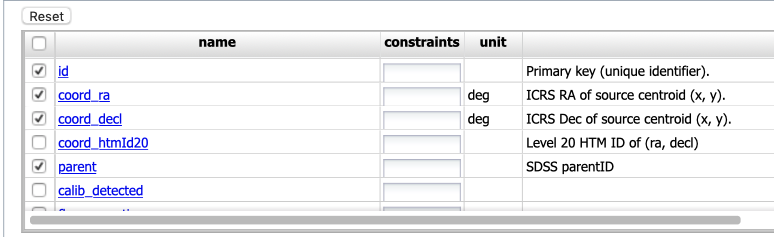
\includegraphics[width=3.12500in]{jira_imgs/244.png}\\

                \vspace{\dp0}
                } \end{minipage} \\ \cdashline{2-3}
                & {\small Test Data} &
                \begin{minipage}[t]{13cm}{\scriptsize
                } \end{minipage} \\ \cdashline{2-3}
                & {\small Expected Result} &
                    \begin{minipage}[t]{13cm}{\scriptsize
                    The column box should be configured to return a minimal useful set of
columns.

                    \vspace{\dp0}
                    } \end{minipage}
                \\ \hdashline


                \multirow{3}{*}{\parbox{1.3cm}{ 2-2
                {\scriptsize from \hyperref[lvv-t851]
                {LVV-T851} } } }

                & {\small Description} &
                \begin{minipage}[t]{13cm}{\scriptsize
                Enter an object name for the portal to resolve. ~We will use NGC 359, a
large elliptical galaxy in the Stripe 82 coverage.\\[2\baselineskip]To
do this, enter the name ``NGC 359'' in the ``Name or Position'' text
input box.\\[2\baselineskip]Leave the other defaults in
place.\\[2\baselineskip]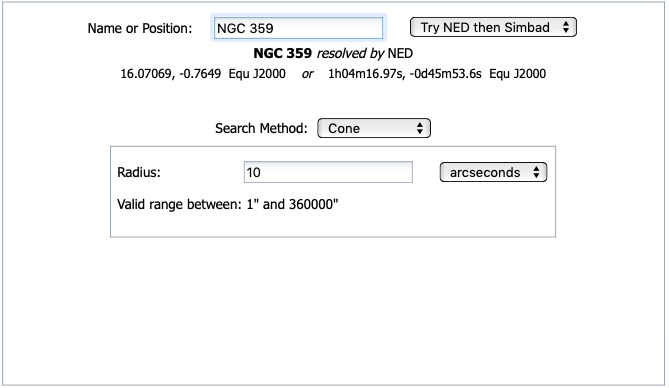
\includegraphics[width=3.12500in]{jira_imgs/245.png}

                \vspace{\dp0}
                } \end{minipage} \\ \cdashline{2-3}
                & {\small Test Data} &
                \begin{minipage}[t]{13cm}{\scriptsize
                } \end{minipage} \\ \cdashline{2-3}
                & {\small Expected Result} &
                    \begin{minipage}[t]{13cm}{\scriptsize
                    There should be a message like ``NGC 359 resolved by NED''. ~The example
coordinates should also changed to the coordinates of NGC 359.

                    \vspace{\dp0}
                    } \end{minipage}
                \\ \hdashline


                \multirow{3}{*}{\parbox{1.3cm}{ 2-3
                {\scriptsize from \hyperref[lvv-t851]
                {LVV-T851} } } }

                & {\small Description} &
                \begin{minipage}[t]{13cm}{\scriptsize
                Submit the query to the portal query engine by clicking the ``Search''
button in the lower left corner of the interface.

                \vspace{\dp0}
                } \end{minipage} \\ \cdashline{2-3}
                & {\small Test Data} &
                \begin{minipage}[t]{13cm}{\scriptsize
                } \end{minipage} \\ \cdashline{2-3}
                & {\small Expected Result} &
                    \begin{minipage}[t]{13cm}{\scriptsize
                    A firefly app with the summary image overlay and catalog widgets side by
side. ~A plot of RA vs. Dec is displayed below the side by side
widgets.\\[2\baselineskip]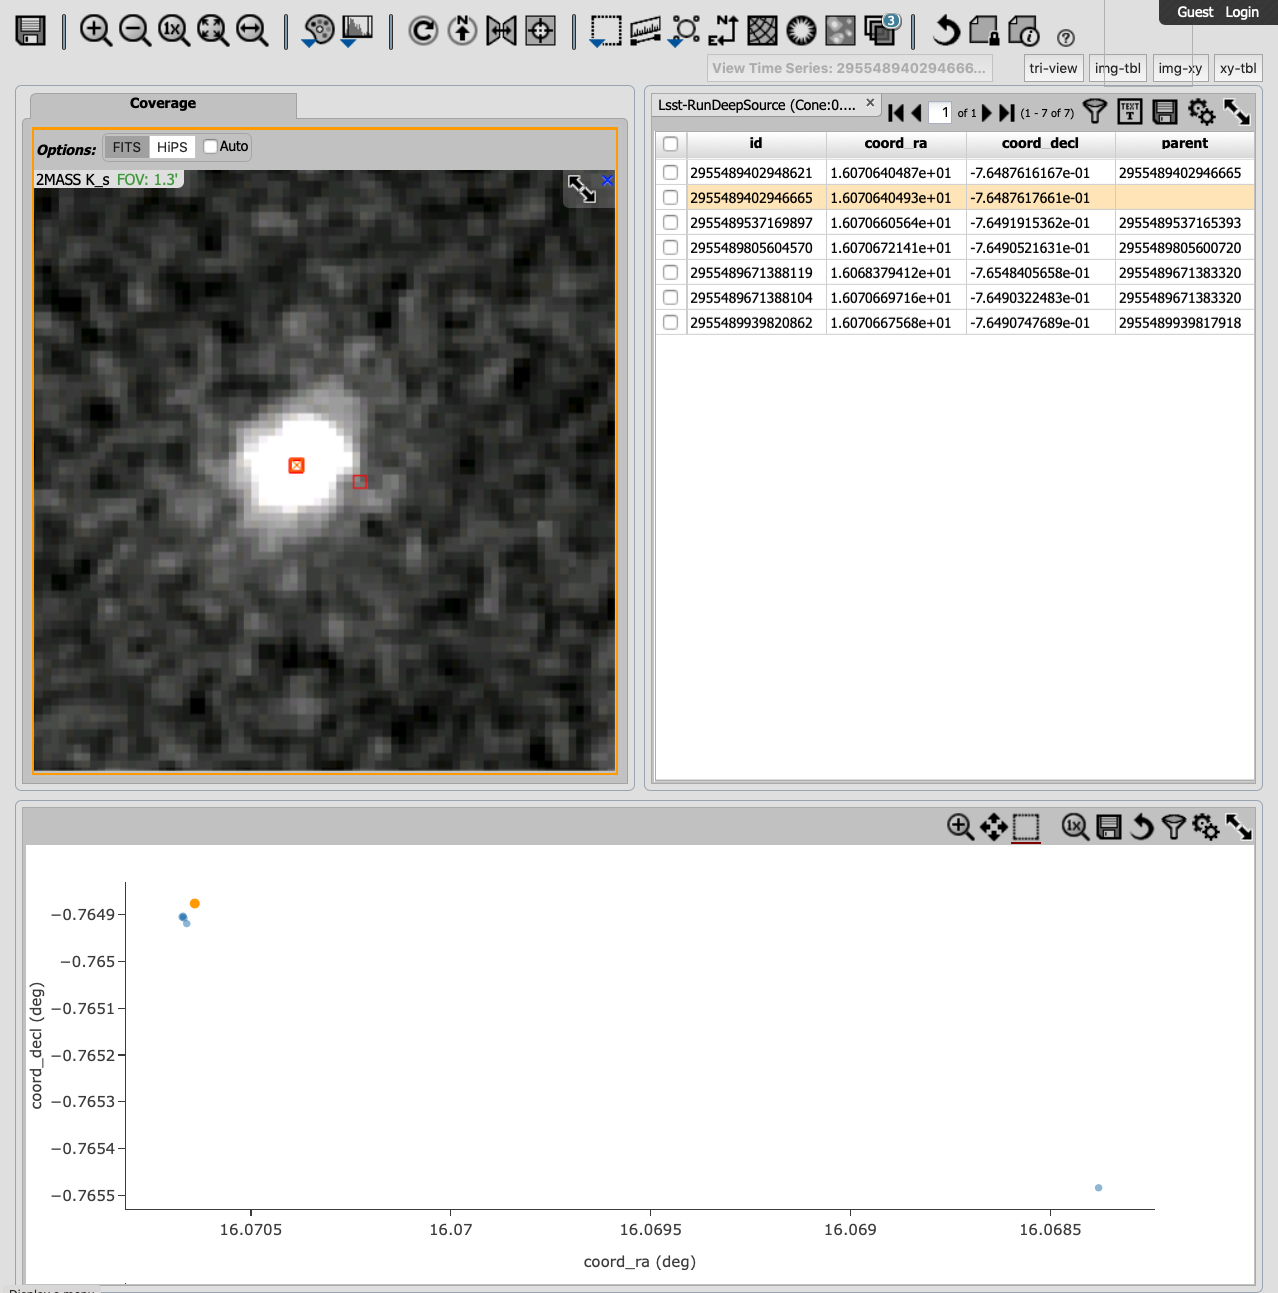
\includegraphics[width=3.12500in]{jira_imgs/246.png}

                    \vspace{\dp0}
                    } \end{minipage}
                \\ \hdashline


        \\ \midrule

                \multirow{3}{*}{\parbox{1.3cm}{ 3-1
                {\scriptsize from \hyperref[lvv-t850]
                {LVV-T850} } } }

                & {\small Description} &
                \begin{minipage}[t]{13cm}{\scriptsize
                Currently, there is no logout mechanism on the portal.\\
This should be updated as the system matures.\\[2\baselineskip]Simply
close the browser window.

                \vspace{\dp0}
                } \end{minipage} \\ \cdashline{2-3}
                & {\small Test Data} &
                \begin{minipage}[t]{13cm}{\scriptsize
                } \end{minipage} \\ \cdashline{2-3}
                & {\small Expected Result} &
                    \begin{minipage}[t]{13cm}{\scriptsize
                    Closed browser window. ~When navigating to the portal endpoint, expect
to execute the steps in LVV-T849.

                    \vspace{\dp0}
                    } \end{minipage}
                \\ \hdashline


        \\ \midrule
    \end{longtable}

\subsection{LVV-T659 - Verify positional query by Source or Object name}\label{lvv-t659}

\begin{longtable}[]{llllll}
\toprule
Version & Status & Priority & Verification Type & Owner
\\\midrule
1 & Draft & Normal &
Test & Jeffrey Carlin
\\\bottomrule
\multicolumn{6}{c}{ Open \href{https://jira.lsstcorp.org/secure/Tests.jspa\#/testCase/LVV-T659}{LVV-T659} in Jira } \\
\end{longtable}

\subsubsection{Verification Elements}
\begin{itemize}
\item \href{https://jira.lsstcorp.org/browse/LVV-9864}{LVV-9864} - DMS-PRTL-REQ-0024-V-01: Positional Query: LSST Object and Source
Identifiers\_1

\end{itemize}

\subsubsection{Test Items}
Verify that positional queries can be performed for coordinates based on
a given object or source ID (e.g., (DIA)Object, (DIA)Source,
ForcedSource).


\subsubsection{Predecessors}

\subsubsection{Environment Needs}

\paragraph{Software}

\paragraph{Hardware}

\subsubsection{Input Specification}

\subsubsection{Output Specification}

\subsubsection{Test Procedure}
    \begin{longtable}[]{p{1.3cm}p{2cm}p{13cm}}
    %\toprule
    Step & \multicolumn{2}{@{}l}{Description, Input Data and Expected Result} \\ \toprule
    \endhead

            \multirow{3}{*}{ 1 } & Description &
            \begin{minipage}[t]{13cm}{\footnotesize
            
            \vspace{\dp0}
            } \end{minipage} \\ \cline{2-3}
            & Test Data &
            \begin{minipage}[t]{13cm}{\footnotesize
                No data.
                \vspace{\dp0}
            } \end{minipage} \\ \cline{2-3}
            & Expected Result &
        \\ \midrule
    \end{longtable}

\subsection{LVV-T660 - Verify positional query based on Solar System object names}\label{lvv-t660}

\begin{longtable}[]{llllll}
\toprule
Version & Status & Priority & Verification Type & Owner
\\\midrule
1 & Draft & Normal &
Test & Jeffrey Carlin
\\\bottomrule
\multicolumn{6}{c}{ Open \href{https://jira.lsstcorp.org/secure/Tests.jspa\#/testCase/LVV-T660}{LVV-T660} in Jira } \\
\end{longtable}

\subsubsection{Verification Elements}
\begin{itemize}
\item \href{https://jira.lsstcorp.org/browse/LVV-9867}{LVV-9867} - DMS-PRTL-REQ-0025-V-01: Positional Query: Solar System Object Names\_1

\end{itemize}

\subsubsection{Test Items}
Verify that positional queries can be performed for coordinates based on
a given Solar System object name.


\subsubsection{Predecessors}

\subsubsection{Environment Needs}

\paragraph{Software}

\paragraph{Hardware}

\subsubsection{Input Specification}

\subsubsection{Output Specification}

\subsubsection{Test Procedure}
    \begin{longtable}[]{p{1.3cm}p{2cm}p{13cm}}
    %\toprule
    Step & \multicolumn{2}{@{}l}{Description, Input Data and Expected Result} \\ \toprule
    \endhead

            \multirow{3}{*}{ 1 } & Description &
            \begin{minipage}[t]{13cm}{\footnotesize
            
            \vspace{\dp0}
            } \end{minipage} \\ \cline{2-3}
            & Test Data &
            \begin{minipage}[t]{13cm}{\footnotesize
                No data.
                \vspace{\dp0}
            } \end{minipage} \\ \cline{2-3}
            & Expected Result &
        \\ \midrule
    \end{longtable}

\subsection{LVV-T661 - Verify query by cone search}\label{lvv-t661}

\begin{longtable}[]{llllll}
\toprule
Version & Status & Priority & Verification Type & Owner
\\\midrule
1 & Draft & Normal &
Test & Jeffrey Carlin
\\\bottomrule
\multicolumn{6}{c}{ Open \href{https://jira.lsstcorp.org/secure/Tests.jspa\#/testCase/LVV-T661}{LVV-T661} in Jira } \\
\end{longtable}

\subsubsection{Verification Elements}
\begin{itemize}
\item \href{https://jira.lsstcorp.org/browse/LVV-9869}{LVV-9869} - DMS-PRTL-REQ-0026-V-01: Positional Query by Region: Cone-Search\_1

\end{itemize}

\subsubsection{Test Items}
Verify that Portal supports position-based queries based on a
cone-shaped radial search.


\subsubsection{Predecessors}

\subsubsection{Environment Needs}

\paragraph{Software}

\paragraph{Hardware}

\subsubsection{Input Specification}

\subsubsection{Output Specification}

\subsubsection{Test Procedure}
    \begin{longtable}[]{p{1.3cm}p{2cm}p{13cm}}
    %\toprule
    Step & \multicolumn{2}{@{}l}{Description, Input Data and Expected Result} \\ \toprule
    \endhead

                \multirow{3}{*}{\parbox{1.3cm}{ 1-1
                {\scriptsize from \hyperref[lvv-t849]
                {LVV-T849} } } }

                & {\small Description} &
                \begin{minipage}[t]{13cm}{\scriptsize
                Navigate to the Portal Aspect endpoint. ~The stable version should be
used for this test and is currently located at:
https://lsst-lsp-stable.ncsa.illinois.edu/portal/app/ .

                \vspace{\dp0}
                } \end{minipage} \\ \cdashline{2-3}
                & {\small Test Data} &
                \begin{minipage}[t]{13cm}{\scriptsize
                } \end{minipage} \\ \cdashline{2-3}
                & {\small Expected Result} &
                    \begin{minipage}[t]{13cm}{\scriptsize
                    A credential-entry screen should be displayed.

                    \vspace{\dp0}
                    } \end{minipage}
                \\ \hdashline


                \multirow{3}{*}{\parbox{1.3cm}{ 1-2
                {\scriptsize from \hyperref[lvv-t849]
                {LVV-T849} } } }

                & {\small Description} &
                \begin{minipage}[t]{13cm}{\scriptsize
                Enter a valid set of credentials for an LSST user with LSP access on the
instance under test.

                \vspace{\dp0}
                } \end{minipage} \\ \cdashline{2-3}
                & {\small Test Data} &
                \begin{minipage}[t]{13cm}{\scriptsize
                } \end{minipage} \\ \cdashline{2-3}
                & {\small Expected Result} &
                    \begin{minipage}[t]{13cm}{\scriptsize
                    The Portal Aspect UI should be displayed following authentication.

                    \vspace{\dp0}
                    } \end{minipage}
                \\ \hdashline


        \\ \midrule

            \multirow{3}{*}{ 2 } & Description &
            \begin{minipage}[t]{13cm}{\footnotesize
            The default catalog (SDSS Stripe 82, 2013 LSST Processing) is fine for
this.\\[2\baselineskip]Choose columns to return by:\\
1) unchecking the top box in the column selection box\\
2) checking columns for id, coord\_ra, coord\_dec, and
parent.\\[2\baselineskip]The result should look like the following:\\
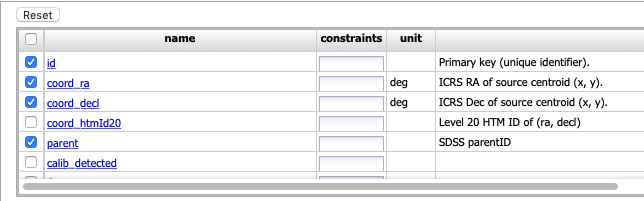
\includegraphics[width=3.12500in]{jira_imgs/247.png}\\

            \vspace{\dp0}
            } \end{minipage} \\ \cline{2-3}
            & Test Data &
            \begin{minipage}[t]{13cm}{\footnotesize
                No data.
                \vspace{\dp0}
            } \end{minipage} \\ \cline{2-3}
            & Expected Result &
                \begin{minipage}[t]{13cm}{\footnotesize
                The column box should be configured to return a minimal useful set of
columns.

                \vspace{\dp0}
                } \end{minipage}
        \\ \midrule

            \multirow{3}{*}{ 3 } & Description &
            \begin{minipage}[t]{13cm}{\footnotesize
            Attempt to access data using sexagesimal format by:\\
1) entering an arbitrary position in the Stripe 82 footprint into the
``Name or Position:'' input text box: 22h2m1s 0d15m0.3s\\
2) change the radius of the query by changing the default value in the
``Radius:'' box to 15.

            \vspace{\dp0}
            } \end{minipage} \\ \cline{2-3}
            & Test Data &
            \begin{minipage}[t]{13cm}{\footnotesize
                No data.
                \vspace{\dp0}
            } \end{minipage} \\ \cline{2-3}
            & Expected Result &
                \begin{minipage}[t]{13cm}{\footnotesize
                The cone search parameters are expected to be configured in a way as to
return data from the service.

                \vspace{\dp0}
                } \end{minipage}
        \\ \midrule

            \multirow{3}{*}{ 4 } & Description &
            \begin{minipage}[t]{13cm}{\footnotesize
            Call the service by clicking the ``Search'' button in the lower left
corner of the interface.

            \vspace{\dp0}
            } \end{minipage} \\ \cline{2-3}
            & Test Data &
            \begin{minipage}[t]{13cm}{\footnotesize
                No data.
                \vspace{\dp0}
            } \end{minipage} \\ \cline{2-3}
            & Expected Result &
                \begin{minipage}[t]{13cm}{\footnotesize
                A firefly instance with the image summary and catalog widgets side by
side with the plot of sky coordinates below:\\
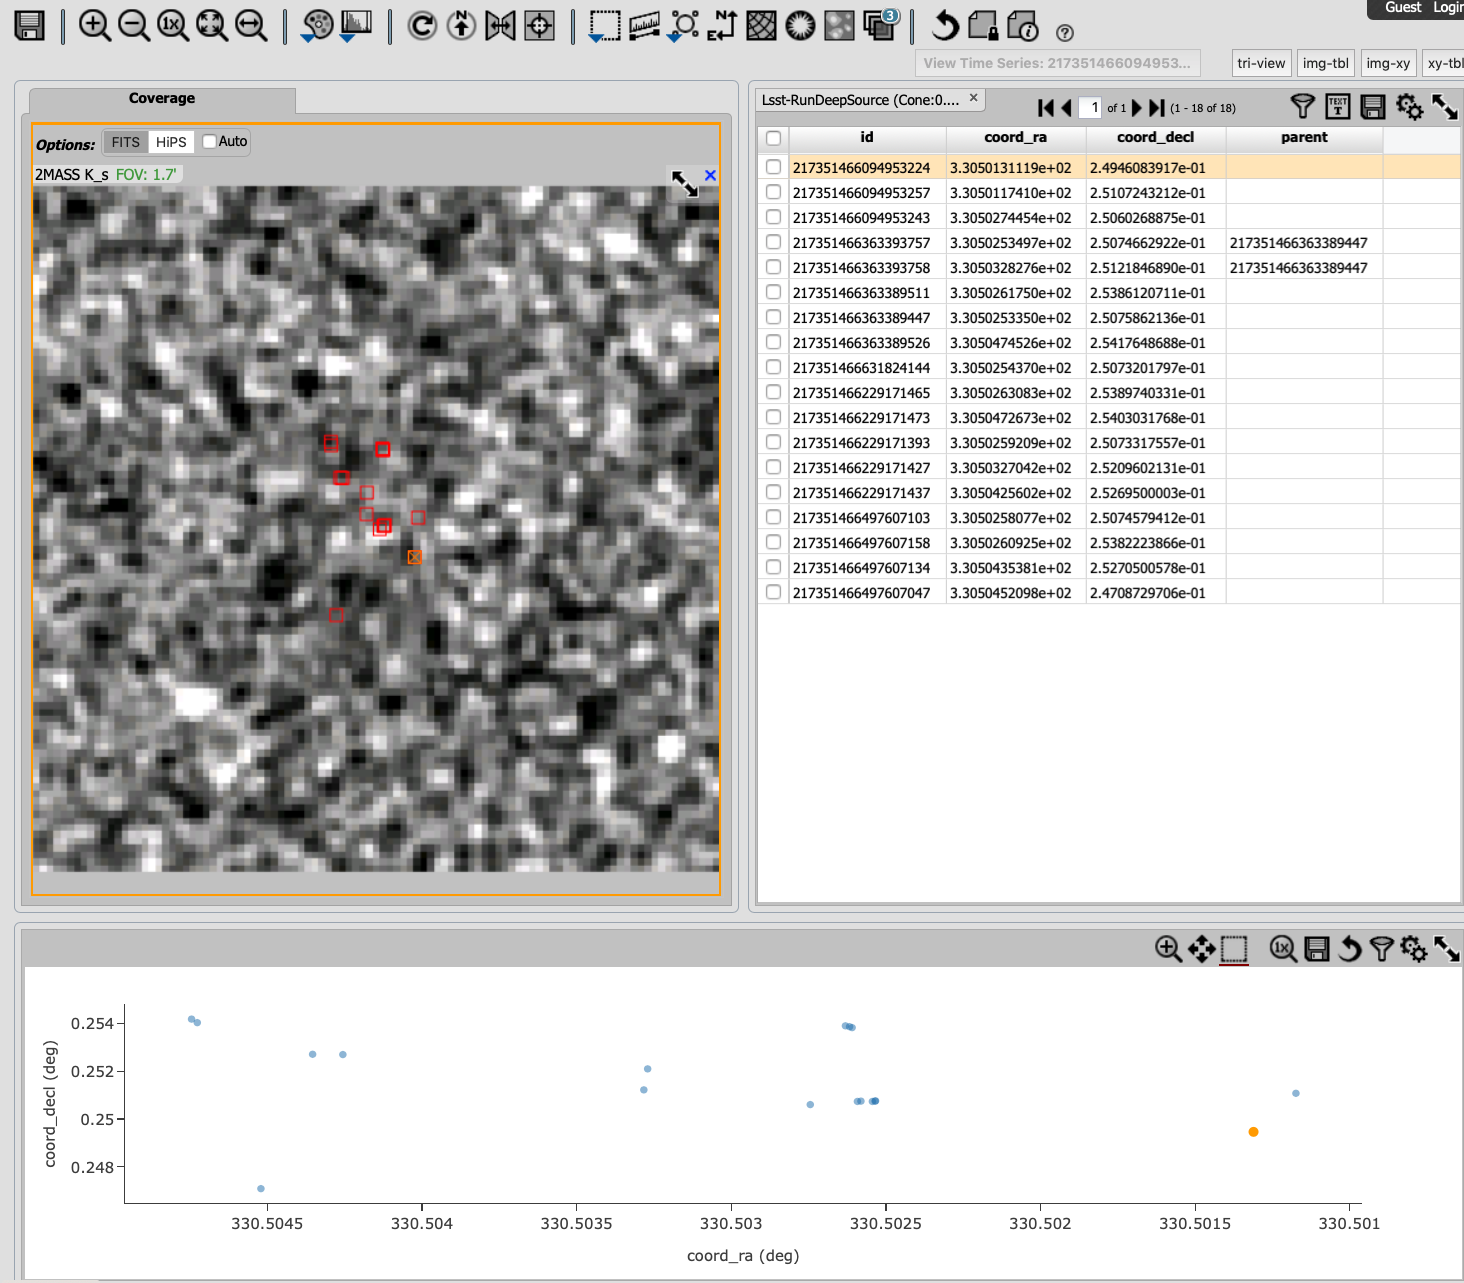
\includegraphics[width=3.12500in]{jira_imgs/248.png}

                \vspace{\dp0}
                } \end{minipage}
        \\ \midrule

            \multirow{3}{*}{ 5 } & Description &
            \begin{minipage}[t]{13cm}{\footnotesize
            Return to the query interface by clicking the ``LSST Data'' button in
the upper left of the interface.

            \vspace{\dp0}
            } \end{minipage} \\ \cline{2-3}
            & Test Data &
            \begin{minipage}[t]{13cm}{\footnotesize
                No data.
                \vspace{\dp0}
            } \end{minipage} \\ \cline{2-3}
            & Expected Result &
                \begin{minipage}[t]{13cm}{\footnotesize
                Expect to be returned to the query interface with the previous search
criteria pre-filled in the appropriate boxes.

                \vspace{\dp0}
                } \end{minipage}
        \\ \midrule

            \multirow{3}{*}{ 6 } & Description &
            \begin{minipage}[t]{13cm}{\footnotesize
            Modify the query to use decimal inputs by changing ``22h2m1s 0d15m0.3s''
to ``330.504167 0.250083''.

            \vspace{\dp0}
            } \end{minipage} \\ \cline{2-3}
            & Test Data &
            \begin{minipage}[t]{13cm}{\footnotesize
                No data.
                \vspace{\dp0}
            } \end{minipage} \\ \cline{2-3}
            & Expected Result &
                \begin{minipage}[t]{13cm}{\footnotesize
                The parameters updated for the decimal format.

                \vspace{\dp0}
                } \end{minipage}
        \\ \midrule

            \multirow{3}{*}{ 7 } & Description &
            \begin{minipage}[t]{13cm}{\footnotesize
            Execute the modified query by clicking the ``Search'' button at the
bottom left of the interface.

            \vspace{\dp0}
            } \end{minipage} \\ \cline{2-3}
            & Test Data &
            \begin{minipage}[t]{13cm}{\footnotesize
                No data.
                \vspace{\dp0}
            } \end{minipage} \\ \cline{2-3}
            & Expected Result &
                \begin{minipage}[t]{13cm}{\footnotesize
                A firefly instance as in step 4 but with two catalog tabs instead of
just one:\\
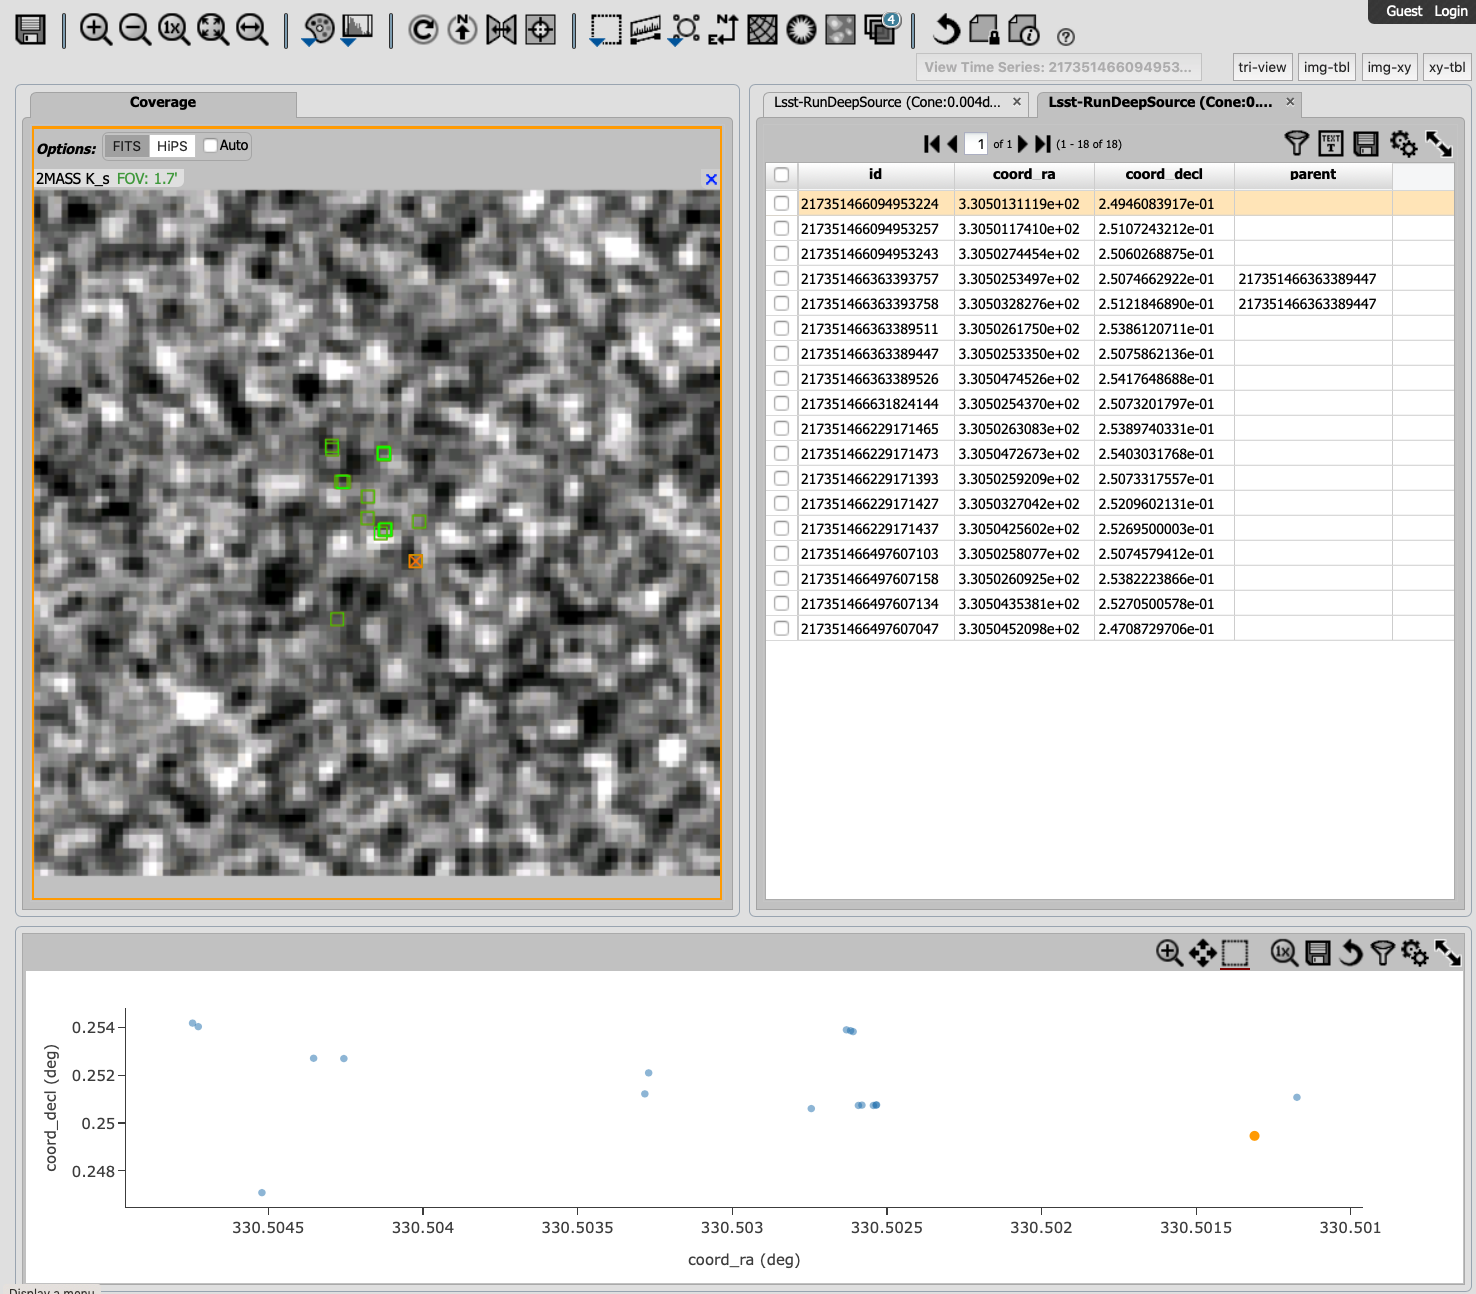
\includegraphics[width=3.12500in]{jira_imgs/249.png}

                \vspace{\dp0}
                } \end{minipage}
        \\ \midrule

            \multirow{3}{*}{ 8 } & Description &
            \begin{minipage}[t]{13cm}{\footnotesize
            Verify the two returned catalogs are the same by clicking between the
two catalog tabs.

            \vspace{\dp0}
            } \end{minipage} \\ \cline{2-3}
            & Test Data &
            \begin{minipage}[t]{13cm}{\footnotesize
                No data.
                \vspace{\dp0}
            } \end{minipage} \\ \cline{2-3}
            & Expected Result &
                \begin{minipage}[t]{13cm}{\footnotesize
                Identical catalogs from the two queries.

                \vspace{\dp0}
                } \end{minipage}
        \\ \midrule

                \multirow{3}{*}{\parbox{1.3cm}{ 9-1
                {\scriptsize from \hyperref[lvv-t850]
                {LVV-T850} } } }

                & {\small Description} &
                \begin{minipage}[t]{13cm}{\scriptsize
                Currently, there is no logout mechanism on the portal.\\
This should be updated as the system matures.\\[2\baselineskip]Simply
close the browser window.

                \vspace{\dp0}
                } \end{minipage} \\ \cdashline{2-3}
                & {\small Test Data} &
                \begin{minipage}[t]{13cm}{\scriptsize
                } \end{minipage} \\ \cdashline{2-3}
                & {\small Expected Result} &
                    \begin{minipage}[t]{13cm}{\scriptsize
                    Closed browser window. ~When navigating to the portal endpoint, expect
to execute the steps in LVV-T849.

                    \vspace{\dp0}
                    } \end{minipage}
                \\ \hdashline


        \\ \midrule
    \end{longtable}

\subsection{LVV-T662 - Verify query by box search}\label{lvv-t662}

\begin{longtable}[]{llllll}
\toprule
Version & Status & Priority & Verification Type & Owner
\\\midrule
1 & Draft & Normal &
Test & Jeffrey Carlin
\\\bottomrule
\multicolumn{6}{c}{ Open \href{https://jira.lsstcorp.org/secure/Tests.jspa\#/testCase/LVV-T662}{LVV-T662} in Jira } \\
\end{longtable}

\subsubsection{Verification Elements}
\begin{itemize}
\item \href{https://jira.lsstcorp.org/browse/LVV-9868}{LVV-9868} - DMS-PRTL-REQ-0027-V-01: Positional Query by Region: Box-Search\_1

\end{itemize}

\subsubsection{Test Items}
Verify that the Portal supports positional queries based on a coordinate
system box search.


\subsubsection{Predecessors}

\subsubsection{Environment Needs}

\paragraph{Software}

\paragraph{Hardware}

\subsubsection{Input Specification}

\subsubsection{Output Specification}

\subsubsection{Test Procedure}
    \begin{longtable}[]{p{1.3cm}p{2cm}p{13cm}}
    %\toprule
    Step & \multicolumn{2}{@{}l}{Description, Input Data and Expected Result} \\ \toprule
    \endhead

            \multirow{3}{*}{ 1 } & Description &
            \begin{minipage}[t]{13cm}{\footnotesize
            
            \vspace{\dp0}
            } \end{minipage} \\ \cline{2-3}
            & Test Data &
            \begin{minipage}[t]{13cm}{\footnotesize
                No data.
                \vspace{\dp0}
            } \end{minipage} \\ \cline{2-3}
            & Expected Result &
        \\ \midrule
    \end{longtable}

\subsection{LVV-T663 - Verify query by time of observation}\label{lvv-t663}

\begin{longtable}[]{llllll}
\toprule
Version & Status & Priority & Verification Type & Owner
\\\midrule
1 & Draft & Normal &
Test & Jeffrey Carlin
\\\bottomrule
\multicolumn{6}{c}{ Open \href{https://jira.lsstcorp.org/secure/Tests.jspa\#/testCase/LVV-T663}{LVV-T663} in Jira } \\
\end{longtable}

\subsubsection{Verification Elements}
\begin{itemize}
\item \href{https://jira.lsstcorp.org/browse/LVV-9870}{LVV-9870} - DMS-PRTL-REQ-0019-V-01: Query by Date and Time: Time Range of
Observation\_1

\end{itemize}

\subsubsection{Test Items}
Verify that the Portal supports queries based on time or ranges of
date/time values in both UT and (barycentric) Julian date.


\subsubsection{Predecessors}

\subsubsection{Environment Needs}

\paragraph{Software}

\paragraph{Hardware}

\subsubsection{Input Specification}

\subsubsection{Output Specification}

\subsubsection{Test Procedure}
    \begin{longtable}[]{p{1.3cm}p{2cm}p{13cm}}
    %\toprule
    Step & \multicolumn{2}{@{}l}{Description, Input Data and Expected Result} \\ \toprule
    \endhead

            \multirow{3}{*}{ 1 } & Description &
            \begin{minipage}[t]{13cm}{\footnotesize
            
            \vspace{\dp0}
            } \end{minipage} \\ \cline{2-3}
            & Test Data &
            \begin{minipage}[t]{13cm}{\footnotesize
                No data.
                \vspace{\dp0}
            } \end{minipage} \\ \cline{2-3}
            & Expected Result &
        \\ \midrule
    \end{longtable}

\subsection{LVV-T664 - Verify implementation of user-friendly tabular query}\label{lvv-t664}

\begin{longtable}[]{llllll}
\toprule
Version & Status & Priority & Verification Type & Owner
\\\midrule
1 & Draft & Normal &
Inspection & Jeffrey Carlin
\\\bottomrule
\multicolumn{6}{c}{ Open \href{https://jira.lsstcorp.org/secure/Tests.jspa\#/testCase/LVV-T664}{LVV-T664} in Jira } \\
\end{longtable}

\subsubsection{Verification Elements}
\begin{itemize}
\item \href{https://jira.lsstcorp.org/browse/LVV-9874}{LVV-9874} - DMS-PRTL-REQ-0031-V-01: Tabular Data Query Specifications\_1

\end{itemize}

\subsubsection{Test Items}
The Portal aspect shall provide a user interface to execute queries of
the (DIA)Object and (DIA)Source tables, driven by the data dictionary
associated with the tables.


\subsubsection{Predecessors}

\subsubsection{Environment Needs}

\paragraph{Software}

\paragraph{Hardware}

\subsubsection{Input Specification}

\subsubsection{Output Specification}

\subsubsection{Test Procedure}
    \begin{longtable}[]{p{1.3cm}p{2cm}p{13cm}}
    %\toprule
    Step & \multicolumn{2}{@{}l}{Description, Input Data and Expected Result} \\ \toprule
    \endhead

            \multirow{3}{*}{ 1 } & Description &
            \begin{minipage}[t]{13cm}{\footnotesize
            
            \vspace{\dp0}
            } \end{minipage} \\ \cline{2-3}
            & Test Data &
            \begin{minipage}[t]{13cm}{\footnotesize
                No data.
                \vspace{\dp0}
            } \end{minipage} \\ \cline{2-3}
            & Expected Result &
        \\ \midrule
    \end{longtable}

\subsection{LVV-T666 - Verify query by image metadata}\label{lvv-t666}

\begin{longtable}[]{llllll}
\toprule
Version & Status & Priority & Verification Type & Owner
\\\midrule
1 & Draft & Normal &
Test & Jeffrey Carlin
\\\bottomrule
\multicolumn{6}{c}{ Open \href{https://jira.lsstcorp.org/secure/Tests.jspa\#/testCase/LVV-T666}{LVV-T666} in Jira } \\
\end{longtable}

\subsubsection{Verification Elements}
\begin{itemize}
\item \href{https://jira.lsstcorp.org/browse/LVV-9873}{LVV-9873} - DMS-PRTL-REQ-0032-V-01: Query Tabular Data based upon Image MetaData\_1

\end{itemize}

\subsubsection{Test Items}
Verify that the Portal supports queries on image metadata (e.g.,
airmass, moon angle, etc.) from the images the catalog measurements were
made from.


\subsubsection{Predecessors}

\subsubsection{Environment Needs}

\paragraph{Software}

\paragraph{Hardware}

\subsubsection{Input Specification}

\subsubsection{Output Specification}

\subsubsection{Test Procedure}
    \begin{longtable}[]{p{1.3cm}p{2cm}p{13cm}}
    %\toprule
    Step & \multicolumn{2}{@{}l}{Description, Input Data and Expected Result} \\ \toprule
    \endhead

            \multirow{3}{*}{ 1 } & Description &
            \begin{minipage}[t]{13cm}{\footnotesize
            
            \vspace{\dp0}
            } \end{minipage} \\ \cline{2-3}
            & Test Data &
            \begin{minipage}[t]{13cm}{\footnotesize
                No data.
                \vspace{\dp0}
            } \end{minipage} \\ \cline{2-3}
            & Expected Result &
        \\ \midrule
    \end{longtable}

\subsection{LVV-T667 - Verify queries on the alerts database}\label{lvv-t667}

\begin{longtable}[]{llllll}
\toprule
Version & Status & Priority & Verification Type & Owner
\\\midrule
1 & Draft & Normal &
Inspection & Jeffrey Carlin
\\\bottomrule
\multicolumn{6}{c}{ Open \href{https://jira.lsstcorp.org/secure/Tests.jspa\#/testCase/LVV-T667}{LVV-T667} in Jira } \\
\end{longtable}

\subsubsection{Verification Elements}
\begin{itemize}
\item \href{https://jira.lsstcorp.org/browse/LVV-9872}{LVV-9872} - DMS-PRTL-REQ-0033-V-01: Queries on the Alerts Database\_1

\end{itemize}

\subsubsection{Test Items}
Verify that the Portal supports queries on parameters in the Alerts
Database.


\subsubsection{Predecessors}

\subsubsection{Environment Needs}

\paragraph{Software}

\paragraph{Hardware}

\subsubsection{Input Specification}

\subsubsection{Output Specification}

\subsubsection{Test Procedure}
    \begin{longtable}[]{p{1.3cm}p{2cm}p{13cm}}
    %\toprule
    Step & \multicolumn{2}{@{}l}{Description, Input Data and Expected Result} \\ \toprule
    \endhead

            \multirow{3}{*}{ 1 } & Description &
            \begin{minipage}[t]{13cm}{\footnotesize
            
            \vspace{\dp0}
            } \end{minipage} \\ \cline{2-3}
            & Test Data &
            \begin{minipage}[t]{13cm}{\footnotesize
                No data.
                \vspace{\dp0}
            } \end{minipage} \\ \cline{2-3}
            & Expected Result &
        \\ \midrule
    \end{longtable}

\subsection{LVV-T668 - Verify access to original alert state}\label{lvv-t668}

\begin{longtable}[]{llllll}
\toprule
Version & Status & Priority & Verification Type & Owner
\\\midrule
1 & Draft & Normal &
Inspection & Jeffrey Carlin
\\\bottomrule
\multicolumn{6}{c}{ Open \href{https://jira.lsstcorp.org/secure/Tests.jspa\#/testCase/LVV-T668}{LVV-T668} in Jira } \\
\end{longtable}

\subsubsection{Verification Elements}
\begin{itemize}
\item \href{https://jira.lsstcorp.org/browse/LVV-9871}{LVV-9871} - DMS-PRTL-REQ-0034-V-01: Access to Original Alert State\_1

\end{itemize}

\subsubsection{Test Items}
Verify that alerts as they were originally raised are accessible via the
Portal.


\subsubsection{Predecessors}

\subsubsection{Environment Needs}

\paragraph{Software}

\paragraph{Hardware}

\subsubsection{Input Specification}

\subsubsection{Output Specification}

\subsubsection{Test Procedure}
    \begin{longtable}[]{p{1.3cm}p{2cm}p{13cm}}
    %\toprule
    Step & \multicolumn{2}{@{}l}{Description, Input Data and Expected Result} \\ \toprule
    \endhead

            \multirow{3}{*}{ 1 } & Description &
            \begin{minipage}[t]{13cm}{\footnotesize
            
            \vspace{\dp0}
            } \end{minipage} \\ \cline{2-3}
            & Test Data &
            \begin{minipage}[t]{13cm}{\footnotesize
                No data.
                \vspace{\dp0}
            } \end{minipage} \\ \cline{2-3}
            & Expected Result &
        \\ \midrule
    \end{longtable}

\subsection{LVV-T669 - Verify query for single-epoch visit images}\label{lvv-t669}

\begin{longtable}[]{llllll}
\toprule
Version & Status & Priority & Verification Type & Owner
\\\midrule
1 & Draft & Normal &
Inspection & Jeffrey Carlin
\\\bottomrule
\multicolumn{6}{c}{ Open \href{https://jira.lsstcorp.org/secure/Tests.jspa\#/testCase/LVV-T669}{LVV-T669} in Jira } \\
\end{longtable}

\subsubsection{Verification Elements}
\begin{itemize}
\item \href{https://jira.lsstcorp.org/browse/LVV-9878}{LVV-9878} - DMS-PRTL-REQ-0035-V-01: Query for Single Epoch Visit Images\_1

\end{itemize}

\subsubsection{Test Items}
Verify that users with a list of visits (either directly, or from a
visit-selection query) can query for single-epoch images corresponding
to those visits.


\subsubsection{Predecessors}

\subsubsection{Environment Needs}

\paragraph{Software}

\paragraph{Hardware}

\subsubsection{Input Specification}

\subsubsection{Output Specification}

\subsubsection{Test Procedure}
    \begin{longtable}[]{p{1.3cm}p{2cm}p{13cm}}
    %\toprule
    Step & \multicolumn{2}{@{}l}{Description, Input Data and Expected Result} \\ \toprule
    \endhead

            \multirow{3}{*}{ 1 } & Description &
            \begin{minipage}[t]{13cm}{\footnotesize
            
            \vspace{\dp0}
            } \end{minipage} \\ \cline{2-3}
            & Test Data &
            \begin{minipage}[t]{13cm}{\footnotesize
                No data.
                \vspace{\dp0}
            } \end{minipage} \\ \cline{2-3}
            & Expected Result &
        \\ \midrule
    \end{longtable}

\subsection{LVV-T670 - Verify query for single-epoch raft images}\label{lvv-t670}

\begin{longtable}[]{llllll}
\toprule
Version & Status & Priority & Verification Type & Owner
\\\midrule
1 & Draft & Normal &
Inspection & Jeffrey Carlin
\\\bottomrule
\multicolumn{6}{c}{ Open \href{https://jira.lsstcorp.org/secure/Tests.jspa\#/testCase/LVV-T670}{LVV-T670} in Jira } \\
\end{longtable}

\subsubsection{Verification Elements}
\begin{itemize}
\item \href{https://jira.lsstcorp.org/browse/LVV-9877}{LVV-9877} - DMS-PRTL-REQ-0036-V-01: Query for Single Epoch Raft Images\_1

\end{itemize}

\subsubsection{Test Items}
Verify that users of the single-epoch query service
(\href{https://jira.lsstcorp.org/browse/LVV-9878}{LVV-9878}) can limit
the returned visit images to only a specified raft.


\subsubsection{Predecessors}

\subsubsection{Environment Needs}

\paragraph{Software}

\paragraph{Hardware}

\subsubsection{Input Specification}

\subsubsection{Output Specification}

\subsubsection{Test Procedure}
    \begin{longtable}[]{p{1.3cm}p{2cm}p{13cm}}
    %\toprule
    Step & \multicolumn{2}{@{}l}{Description, Input Data and Expected Result} \\ \toprule
    \endhead

            \multirow{3}{*}{ 1 } & Description &
            \begin{minipage}[t]{13cm}{\footnotesize
            
            \vspace{\dp0}
            } \end{minipage} \\ \cline{2-3}
            & Test Data &
            \begin{minipage}[t]{13cm}{\footnotesize
                No data.
                \vspace{\dp0}
            } \end{minipage} \\ \cline{2-3}
            & Expected Result &
        \\ \midrule
    \end{longtable}

\subsection{LVV-T671 - Verify query for single-epoch CCD images}\label{lvv-t671}

\begin{longtable}[]{llllll}
\toprule
Version & Status & Priority & Verification Type & Owner
\\\midrule
1 & Draft & Normal &
Inspection & Jeffrey Carlin
\\\bottomrule
\multicolumn{6}{c}{ Open \href{https://jira.lsstcorp.org/secure/Tests.jspa\#/testCase/LVV-T671}{LVV-T671} in Jira } \\
\end{longtable}

\subsubsection{Verification Elements}
\begin{itemize}
\item \href{https://jira.lsstcorp.org/browse/LVV-9876}{LVV-9876} - DMS-PRTL-REQ-0037-V-01: Query for Single Epoch CCD Image\_1

\end{itemize}

\subsubsection{Test Items}
Verify that users of the single-epoch query service
(\href{https://jira.lsstcorp.org/browse/LVV-9878}{LVV-9878}) can limit
the returned visit images to only a specified CCD.


\subsubsection{Predecessors}

\subsubsection{Environment Needs}

\paragraph{Software}

\paragraph{Hardware}

\subsubsection{Input Specification}

\subsubsection{Output Specification}

\subsubsection{Test Procedure}
    \begin{longtable}[]{p{1.3cm}p{2cm}p{13cm}}
    %\toprule
    Step & \multicolumn{2}{@{}l}{Description, Input Data and Expected Result} \\ \toprule
    \endhead

            \multirow{3}{*}{ 1 } & Description &
            \begin{minipage}[t]{13cm}{\footnotesize
            
            \vspace{\dp0}
            } \end{minipage} \\ \cline{2-3}
            & Test Data &
            \begin{minipage}[t]{13cm}{\footnotesize
                No data.
                \vspace{\dp0}
            } \end{minipage} \\ \cline{2-3}
            & Expected Result &
        \\ \midrule
    \end{longtable}

\subsection{LVV-T672 - Verify metadata query for single-epoch images}\label{lvv-t672}

\begin{longtable}[]{llllll}
\toprule
Version & Status & Priority & Verification Type & Owner
\\\midrule
1 & Draft & Normal &
Inspection & Jeffrey Carlin
\\\bottomrule
\multicolumn{6}{c}{ Open \href{https://jira.lsstcorp.org/secure/Tests.jspa\#/testCase/LVV-T672}{LVV-T672} in Jira } \\
\end{longtable}

\subsubsection{Verification Elements}
\begin{itemize}
\item \href{https://jira.lsstcorp.org/browse/LVV-9879}{LVV-9879} - DMS-PRTL-REQ-0038-V-01: Single-Epoch Image Query Specifications\_1

\end{itemize}

\subsubsection{Test Items}
Verify that the Portal provides an option to query for visits and
single-epoch images of a certain type based on image metadata or
parameters from the reformatted EFD.


\subsubsection{Predecessors}

\subsubsection{Environment Needs}

\paragraph{Software}

\paragraph{Hardware}

\subsubsection{Input Specification}

\subsubsection{Output Specification}

\subsubsection{Test Procedure}
    \begin{longtable}[]{p{1.3cm}p{2cm}p{13cm}}
    %\toprule
    Step & \multicolumn{2}{@{}l}{Description, Input Data and Expected Result} \\ \toprule
    \endhead

            \multirow{3}{*}{ 1 } & Description &
            \begin{minipage}[t]{13cm}{\footnotesize
            
            \vspace{\dp0}
            } \end{minipage} \\ \cline{2-3}
            & Test Data &
            \begin{minipage}[t]{13cm}{\footnotesize
                No data.
                \vspace{\dp0}
            } \end{minipage} \\ \cline{2-3}
            & Expected Result &
        \\ \midrule
    \end{longtable}

\subsection{LVV-T673 - Verify query for coadds by image metadata}\label{lvv-t673}

\begin{longtable}[]{llllll}
\toprule
Version & Status & Priority & Verification Type & Owner
\\\midrule
1 & Draft & Normal &
Inspection & Jeffrey Carlin
\\\bottomrule
\multicolumn{6}{c}{ Open \href{https://jira.lsstcorp.org/secure/Tests.jspa\#/testCase/LVV-T673}{LVV-T673} in Jira } \\
\end{longtable}

\subsubsection{Verification Elements}
\begin{itemize}
\item \href{https://jira.lsstcorp.org/browse/LVV-9875}{LVV-9875} - DMS-PRTL-REQ-0039-V-01: Coadded Image Query Specifications\_1

\end{itemize}

\subsubsection{Test Items}
Verify that the Portal aspect supports queries based on image metadata
describing the provenance of the contributing images, that return the
corresponding coadd image(s).


\subsubsection{Predecessors}

\subsubsection{Environment Needs}

\paragraph{Software}

\paragraph{Hardware}

\subsubsection{Input Specification}

\subsubsection{Output Specification}

\subsubsection{Test Procedure}
    \begin{longtable}[]{p{1.3cm}p{2cm}p{13cm}}
    %\toprule
    Step & \multicolumn{2}{@{}l}{Description, Input Data and Expected Result} \\ \toprule
    \endhead

            \multirow{3}{*}{ 1 } & Description &
            \begin{minipage}[t]{13cm}{\footnotesize
            
            \vspace{\dp0}
            } \end{minipage} \\ \cline{2-3}
            & Test Data &
            \begin{minipage}[t]{13cm}{\footnotesize
                No data.
                \vspace{\dp0}
            } \end{minipage} \\ \cline{2-3}
            & Expected Result &
        \\ \midrule
    \end{longtable}

\subsection{LVV-T674 - Verify query for coadd image cutouts}\label{lvv-t674}

\begin{longtable}[]{llllll}
\toprule
Version & Status & Priority & Verification Type & Owner
\\\midrule
1 & Draft & Normal &
Inspection & Jeffrey Carlin
\\\bottomrule
\multicolumn{6}{c}{ Open \href{https://jira.lsstcorp.org/secure/Tests.jspa\#/testCase/LVV-T674}{LVV-T674} in Jira } \\
\end{longtable}

\subsubsection{Verification Elements}
\begin{itemize}
\item \href{https://jira.lsstcorp.org/browse/LVV-9880}{LVV-9880} - DMS-PRTL-REQ-0041-V-01: Query for Coadded Image Cutouts\_1

\end{itemize}

\subsubsection{Test Items}
Verify that Portal users can query based on image metadata for coadds,
then obtain a list of sub-images (cutouts) with a specified center
position and size.


\subsubsection{Predecessors}

\subsubsection{Environment Needs}

\paragraph{Software}

\paragraph{Hardware}

\subsubsection{Input Specification}

\subsubsection{Output Specification}

\subsubsection{Test Procedure}
    \begin{longtable}[]{p{1.3cm}p{2cm}p{13cm}}
    %\toprule
    Step & \multicolumn{2}{@{}l}{Description, Input Data and Expected Result} \\ \toprule
    \endhead

            \multirow{3}{*}{ 1 } & Description &
            \begin{minipage}[t]{13cm}{\footnotesize
            
            \vspace{\dp0}
            } \end{minipage} \\ \cline{2-3}
            & Test Data &
            \begin{minipage}[t]{13cm}{\footnotesize
                No data.
                \vspace{\dp0}
            } \end{minipage} \\ \cline{2-3}
            & Expected Result &
        \\ \midrule
    \end{longtable}

\subsection{LVV-T675 - Verify query for single-epoch image cutouts}\label{lvv-t675}

\begin{longtable}[]{llllll}
\toprule
Version & Status & Priority & Verification Type & Owner
\\\midrule
1 & Draft & Normal &
Inspection & Jeffrey Carlin
\\\bottomrule
\multicolumn{6}{c}{ Open \href{https://jira.lsstcorp.org/secure/Tests.jspa\#/testCase/LVV-T675}{LVV-T675} in Jira } \\
\end{longtable}

\subsubsection{Verification Elements}
\begin{itemize}
\item \href{https://jira.lsstcorp.org/browse/LVV-9881}{LVV-9881} - DMS-PRTL-REQ-0040-V-01: Query for Single Epoch Image Cutouts\_1

\end{itemize}

\subsubsection{Test Items}
Verify that Portal users can query based on image metadata for
single-epoch images, then obtain a list of sub-images (cutouts) with a
specified center position and size.


\subsubsection{Predecessors}

\subsubsection{Environment Needs}

\paragraph{Software}

\paragraph{Hardware}

\subsubsection{Input Specification}

\subsubsection{Output Specification}

\subsubsection{Test Procedure}
    \begin{longtable}[]{p{1.3cm}p{2cm}p{13cm}}
    %\toprule
    Step & \multicolumn{2}{@{}l}{Description, Input Data and Expected Result} \\ \toprule
    \endhead

            \multirow{3}{*}{ 1 } & Description &
            \begin{minipage}[t]{13cm}{\footnotesize
            
            \vspace{\dp0}
            } \end{minipage} \\ \cline{2-3}
            & Test Data &
            \begin{minipage}[t]{13cm}{\footnotesize
                No data.
                \vspace{\dp0}
            } \end{minipage} \\ \cline{2-3}
            & Expected Result &
        \\ \midrule
    \end{longtable}

\subsection{LVV-T676 - Verify display of native single-visit images}\label{lvv-t676}

\begin{longtable}[]{llllll}
\toprule
Version & Status & Priority & Verification Type & Owner
\\\midrule
1 & Draft & Normal &
Inspection & Jeffrey Carlin
\\\bottomrule
\multicolumn{6}{c}{ Open \href{https://jira.lsstcorp.org/secure/Tests.jspa\#/testCase/LVV-T676}{LVV-T676} in Jira } \\
\end{longtable}

\subsubsection{Verification Elements}
\begin{itemize}
\item \href{https://jira.lsstcorp.org/browse/LVV-9905}{LVV-9905} - DMS-PRTL-REQ-0062-V-01: Display Native Single-Visit Image Data
Products\_1

\end{itemize}

\subsubsection{Test Items}
Verify that the Portal aspect provides a means to display the native
single-visit image data products, including raw images, Processed Visit
Images (PVIs), and difference images, as well as the standard
single-exposure calibration images used as inputs for flats, bias
frames, etc.


\subsubsection{Predecessors}

\subsubsection{Environment Needs}

\paragraph{Software}

\paragraph{Hardware}

\subsubsection{Input Specification}

\subsubsection{Output Specification}

\subsubsection{Test Procedure}
    \begin{longtable}[]{p{1.3cm}p{2cm}p{13cm}}
    %\toprule
    Step & \multicolumn{2}{@{}l}{Description, Input Data and Expected Result} \\ \toprule
    \endhead

            \multirow{3}{*}{ 1 } & Description &
            \begin{minipage}[t]{13cm}{\footnotesize
            
            \vspace{\dp0}
            } \end{minipage} \\ \cline{2-3}
            & Test Data &
            \begin{minipage}[t]{13cm}{\footnotesize
                No data.
                \vspace{\dp0}
            } \end{minipage} \\ \cline{2-3}
            & Expected Result &
        \\ \midrule
    \end{longtable}

\subsection{LVV-T677 - Verify Portal provides visualization of tabular and image data}\label{lvv-t677}

\begin{longtable}[]{llllll}
\toprule
Version & Status & Priority & Verification Type & Owner
\\\midrule
1 & Draft & Normal &
Inspection & Jeffrey Carlin
\\\bottomrule
\multicolumn{6}{c}{ Open \href{https://jira.lsstcorp.org/secure/Tests.jspa\#/testCase/LVV-T677}{LVV-T677} in Jira } \\
\end{longtable}

\subsubsection{Verification Elements}
\begin{itemize}
\item \href{https://jira.lsstcorp.org/browse/LVV-9884}{LVV-9884} - DMS-PRTL-REQ-0042-V-01: Visualization of Tabular and Image Data\_1

\end{itemize}

\subsubsection{Test Items}
Verify that the Portal aspect provides the capability to visualize all
tabular and image data defined in the DPDD, as well as user data
products.


\subsubsection{Predecessors}

\subsubsection{Environment Needs}

\paragraph{Software}

\paragraph{Hardware}

\subsubsection{Input Specification}

\subsubsection{Output Specification}

\subsubsection{Test Procedure}
    \begin{longtable}[]{p{1.3cm}p{2cm}p{13cm}}
    %\toprule
    Step & \multicolumn{2}{@{}l}{Description, Input Data and Expected Result} \\ \toprule
    \endhead

                \multirow{3}{*}{\parbox{1.3cm}{ 1-1
                {\scriptsize from \hyperref[lvv-t849]
                {LVV-T849} } } }

                & {\small Description} &
                \begin{minipage}[t]{13cm}{\scriptsize
                Navigate to the Portal Aspect endpoint. ~The stable version should be
used for this test and is currently located at:
https://lsst-lsp-stable.ncsa.illinois.edu/portal/app/ .

                \vspace{\dp0}
                } \end{minipage} \\ \cdashline{2-3}
                & {\small Test Data} &
                \begin{minipage}[t]{13cm}{\scriptsize
                } \end{minipage} \\ \cdashline{2-3}
                & {\small Expected Result} &
                    \begin{minipage}[t]{13cm}{\scriptsize
                    A credential-entry screen should be displayed.

                    \vspace{\dp0}
                    } \end{minipage}
                \\ \hdashline


                \multirow{3}{*}{\parbox{1.3cm}{ 1-2
                {\scriptsize from \hyperref[lvv-t849]
                {LVV-T849} } } }

                & {\small Description} &
                \begin{minipage}[t]{13cm}{\scriptsize
                Enter a valid set of credentials for an LSST user with LSP access on the
instance under test.

                \vspace{\dp0}
                } \end{minipage} \\ \cdashline{2-3}
                & {\small Test Data} &
                \begin{minipage}[t]{13cm}{\scriptsize
                } \end{minipage} \\ \cdashline{2-3}
                & {\small Expected Result} &
                    \begin{minipage}[t]{13cm}{\scriptsize
                    The Portal Aspect UI should be displayed following authentication.

                    \vspace{\dp0}
                    } \end{minipage}
                \\ \hdashline


        \\ \midrule

                \multirow{3}{*}{\parbox{1.3cm}{ 2-1
                {\scriptsize from \hyperref[lvv-t851]
                {LVV-T851} } } }

                & {\small Description} &
                \begin{minipage}[t]{13cm}{\scriptsize
                The default catalog (SDSS Stripe 82, 2013 LSST Processing) is fine for
this.\\[2\baselineskip]Choose columns to return by:\\
1) unchecking the top box in the column selection box\\
2) checking columns for id, coord\_ra, coord\_dec, and
parent.\\[2\baselineskip]The result should look like the following:\\
\hspace*{0.333em}\\
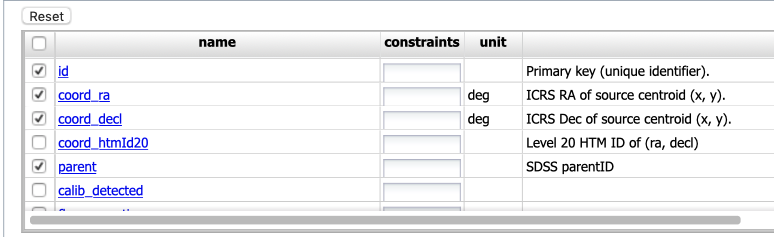
\includegraphics[width=3.12500in]{jira_imgs/244.png}\\

                \vspace{\dp0}
                } \end{minipage} \\ \cdashline{2-3}
                & {\small Test Data} &
                \begin{minipage}[t]{13cm}{\scriptsize
                } \end{minipage} \\ \cdashline{2-3}
                & {\small Expected Result} &
                    \begin{minipage}[t]{13cm}{\scriptsize
                    The column box should be configured to return a minimal useful set of
columns.

                    \vspace{\dp0}
                    } \end{minipage}
                \\ \hdashline


                \multirow{3}{*}{\parbox{1.3cm}{ 2-2
                {\scriptsize from \hyperref[lvv-t851]
                {LVV-T851} } } }

                & {\small Description} &
                \begin{minipage}[t]{13cm}{\scriptsize
                Enter an object name for the portal to resolve. ~We will use NGC 359, a
large elliptical galaxy in the Stripe 82 coverage.\\[2\baselineskip]To
do this, enter the name ``NGC 359'' in the ``Name or Position'' text
input box.\\[2\baselineskip]Leave the other defaults in
place.\\[2\baselineskip]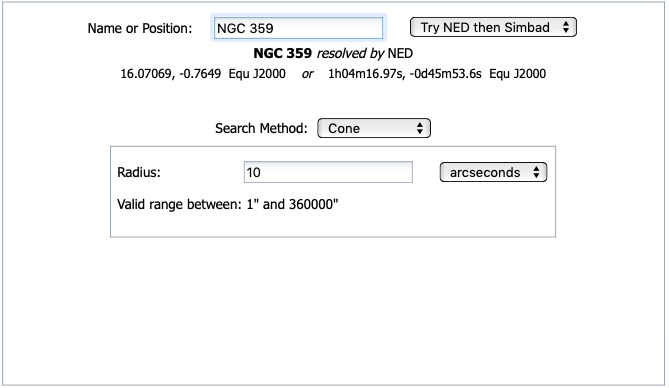
\includegraphics[width=3.12500in]{jira_imgs/245.png}

                \vspace{\dp0}
                } \end{minipage} \\ \cdashline{2-3}
                & {\small Test Data} &
                \begin{minipage}[t]{13cm}{\scriptsize
                } \end{minipage} \\ \cdashline{2-3}
                & {\small Expected Result} &
                    \begin{minipage}[t]{13cm}{\scriptsize
                    There should be a message like ``NGC 359 resolved by NED''. ~The example
coordinates should also changed to the coordinates of NGC 359.

                    \vspace{\dp0}
                    } \end{minipage}
                \\ \hdashline


                \multirow{3}{*}{\parbox{1.3cm}{ 2-3
                {\scriptsize from \hyperref[lvv-t851]
                {LVV-T851} } } }

                & {\small Description} &
                \begin{minipage}[t]{13cm}{\scriptsize
                Submit the query to the portal query engine by clicking the ``Search''
button in the lower left corner of the interface.

                \vspace{\dp0}
                } \end{minipage} \\ \cdashline{2-3}
                & {\small Test Data} &
                \begin{minipage}[t]{13cm}{\scriptsize
                } \end{minipage} \\ \cdashline{2-3}
                & {\small Expected Result} &
                    \begin{minipage}[t]{13cm}{\scriptsize
                    A firefly app with the summary image overlay and catalog widgets side by
side. ~A plot of RA vs. Dec is displayed below the side by side
widgets.\\[2\baselineskip]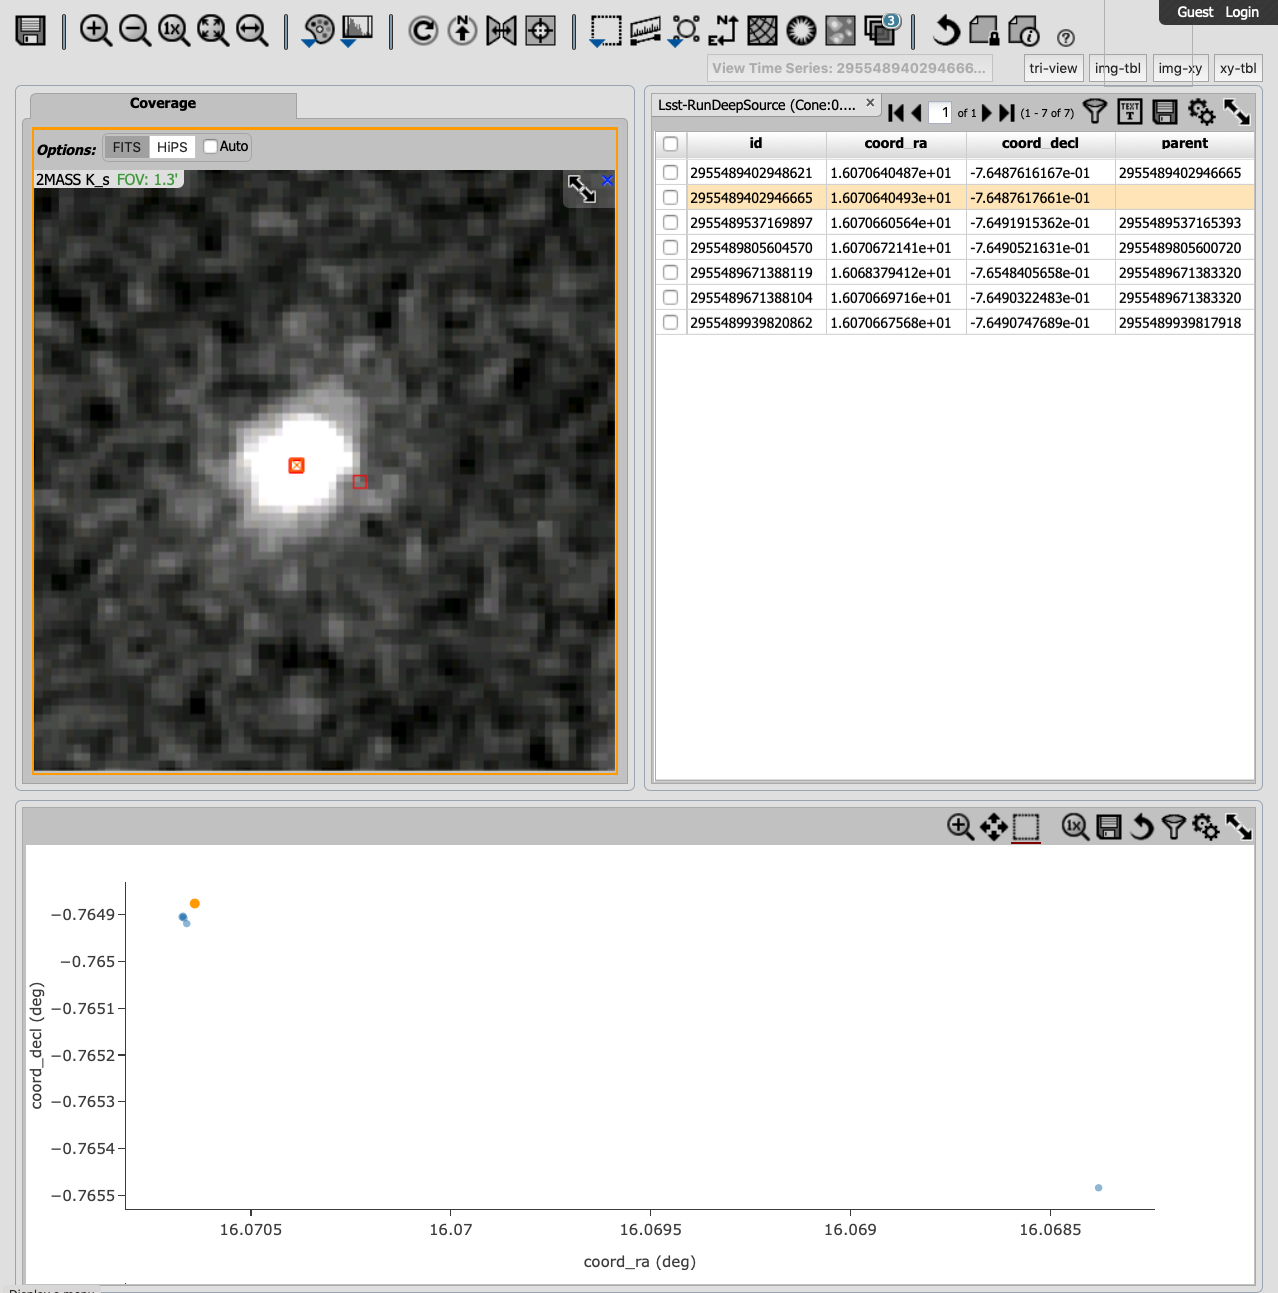
\includegraphics[width=3.12500in]{jira_imgs/246.png}

                    \vspace{\dp0}
                    } \end{minipage}
                \\ \hdashline


        \\ \midrule

            \multirow{3}{*}{ 3 } & Description &
            \begin{minipage}[t]{13cm}{\footnotesize
            Examine tabular view to verify that the selected quantities are
displayed.

            \vspace{\dp0}
            } \end{minipage} \\ \cline{2-3}
            & Test Data &
            \begin{minipage}[t]{13cm}{\footnotesize
                No data.
                \vspace{\dp0}
            } \end{minipage} \\ \cline{2-3}
            & Expected Result &
                \begin{minipage}[t]{13cm}{\footnotesize
                An interactive view

                \vspace{\dp0}
                } \end{minipage}
        \\ \midrule
    \end{longtable}

\subsection{LVV-T678 - Verify visualization of ancillary information}\label{lvv-t678}

\begin{longtable}[]{llllll}
\toprule
Version & Status & Priority & Verification Type & Owner
\\\midrule
1 & Draft & Normal &
Inspection & Jeffrey Carlin
\\\bottomrule
\multicolumn{6}{c}{ Open \href{https://jira.lsstcorp.org/secure/Tests.jspa\#/testCase/LVV-T678}{LVV-T678} in Jira } \\
\end{longtable}

\subsubsection{Verification Elements}
\begin{itemize}
\item \href{https://jira.lsstcorp.org/browse/LVV-9883}{LVV-9883} - DMS-PRTL-REQ-0043-V-01: Visualization of Ancillary Information\_1

\end{itemize}

\subsubsection{Test Items}
Verify that the Portal provides the ability to visualize certain
ancillary information produced by the LSST pipeline, including, but not
limited to, image regions, image bit-planes, survey footprints,
focal-plane footprints and PSF representations.


\subsubsection{Predecessors}

\subsubsection{Environment Needs}

\paragraph{Software}

\paragraph{Hardware}

\subsubsection{Input Specification}

\subsubsection{Output Specification}

\subsubsection{Test Procedure}
    \begin{longtable}[]{p{1.3cm}p{2cm}p{13cm}}
    %\toprule
    Step & \multicolumn{2}{@{}l}{Description, Input Data and Expected Result} \\ \toprule
    \endhead

            \multirow{3}{*}{ 1 } & Description &
            \begin{minipage}[t]{13cm}{\footnotesize
            
            \vspace{\dp0}
            } \end{minipage} \\ \cline{2-3}
            & Test Data &
            \begin{minipage}[t]{13cm}{\footnotesize
                No data.
                \vspace{\dp0}
            } \end{minipage} \\ \cline{2-3}
            & Expected Result &
        \\ \midrule
    \end{longtable}

\subsection{LVV-T679 - Verify visualization linking image and tabular data}\label{lvv-t679}

\begin{longtable}[]{llllll}
\toprule
Version & Status & Priority & Verification Type & Owner
\\\midrule
1 & Draft & Normal &
Inspection & Jeffrey Carlin
\\\bottomrule
\multicolumn{6}{c}{ Open \href{https://jira.lsstcorp.org/secure/Tests.jspa\#/testCase/LVV-T679}{LVV-T679} in Jira } \\
\end{longtable}

\subsubsection{Verification Elements}
\begin{itemize}
\item \href{https://jira.lsstcorp.org/browse/LVV-9882}{LVV-9882} - DMS-PRTL-REQ-0044-V-01: Linking Visualization of Image Data to Tabular
Data\_1

\end{itemize}

\subsubsection{Test Items}
Verify that the Portal aspect provides a capability for users to
navigate between visualization and tabular data for a given tabular
entry.


\subsubsection{Predecessors}

\subsubsection{Environment Needs}

\paragraph{Software}

\paragraph{Hardware}

\subsubsection{Input Specification}

\subsubsection{Output Specification}

\subsubsection{Test Procedure}
    \begin{longtable}[]{p{1.3cm}p{2cm}p{13cm}}
    %\toprule
    Step & \multicolumn{2}{@{}l}{Description, Input Data and Expected Result} \\ \toprule
    \endhead

            \multirow{3}{*}{ 1 } & Description &
            \begin{minipage}[t]{13cm}{\footnotesize
            
            \vspace{\dp0}
            } \end{minipage} \\ \cline{2-3}
            & Test Data &
            \begin{minipage}[t]{13cm}{\footnotesize
                No data.
                \vspace{\dp0}
            } \end{minipage} \\ \cline{2-3}
            & Expected Result &
        \\ \midrule
    \end{longtable}

\subsection{LVV-T680 - Verify visualization tool for uploaded tabular or image data}\label{lvv-t680}

\begin{longtable}[]{llllll}
\toprule
Version & Status & Priority & Verification Type & Owner
\\\midrule
1 & Draft & Normal &
Inspection & Jeffrey Carlin
\\\bottomrule
\multicolumn{6}{c}{ Open \href{https://jira.lsstcorp.org/secure/Tests.jspa\#/testCase/LVV-T680}{LVV-T680} in Jira } \\
\end{longtable}

\subsubsection{Verification Elements}
\begin{itemize}
\item \href{https://jira.lsstcorp.org/browse/LVV-9885}{LVV-9885} - DMS-PRTL-REQ-0045-V-01: Visualization of Uploaded Tabular and Image
Data\_1

\end{itemize}

\subsubsection{Test Items}
Verify that the Portal provides a means of visualizing uploaded tables
or images.


\subsubsection{Predecessors}

\subsubsection{Environment Needs}

\paragraph{Software}

\paragraph{Hardware}

\subsubsection{Input Specification}

\subsubsection{Output Specification}

\subsubsection{Test Procedure}
    \begin{longtable}[]{p{1.3cm}p{2cm}p{13cm}}
    %\toprule
    Step & \multicolumn{2}{@{}l}{Description, Input Data and Expected Result} \\ \toprule
    \endhead

            \multirow{3}{*}{ 1 } & Description &
            \begin{minipage}[t]{13cm}{\footnotesize
            
            \vspace{\dp0}
            } \end{minipage} \\ \cline{2-3}
            & Test Data &
            \begin{minipage}[t]{13cm}{\footnotesize
                No data.
                \vspace{\dp0}
            } \end{minipage} \\ \cline{2-3}
            & Expected Result &
        \\ \midrule
    \end{longtable}

\subsection{LVV-T681 - Verify visualization of workspace data}\label{lvv-t681}

\begin{longtable}[]{llllll}
\toprule
Version & Status & Priority & Verification Type & Owner
\\\midrule
1 & Draft & Normal &
Inspection & Jeffrey Carlin
\\\bottomrule
\multicolumn{6}{c}{ Open \href{https://jira.lsstcorp.org/secure/Tests.jspa\#/testCase/LVV-T681}{LVV-T681} in Jira } \\
\end{longtable}

\subsubsection{Verification Elements}
\begin{itemize}
\item \href{https://jira.lsstcorp.org/browse/LVV-9886}{LVV-9886} - DMS-PRTL-REQ-0046-V-01: Visualization of Workspace Data\_1

\end{itemize}

\subsubsection{Test Items}
Verify that data selected in a workspace browser can be conveniently
visualized.


\subsubsection{Predecessors}

\subsubsection{Environment Needs}

\paragraph{Software}

\paragraph{Hardware}

\subsubsection{Input Specification}

\subsubsection{Output Specification}

\subsubsection{Test Procedure}
    \begin{longtable}[]{p{1.3cm}p{2cm}p{13cm}}
    %\toprule
    Step & \multicolumn{2}{@{}l}{Description, Input Data and Expected Result} \\ \toprule
    \endhead

            \multirow{3}{*}{ 1 } & Description &
            \begin{minipage}[t]{13cm}{\footnotesize
            
            \vspace{\dp0}
            } \end{minipage} \\ \cline{2-3}
            & Test Data &
            \begin{minipage}[t]{13cm}{\footnotesize
                No data.
                \vspace{\dp0}
            } \end{minipage} \\ \cline{2-3}
            & Expected Result &
        \\ \midrule
    \end{longtable}

\subsection{LVV-T682 - Verify availability of property sheets for table rows}\label{lvv-t682}

\begin{longtable}[]{llllll}
\toprule
Version & Status & Priority & Verification Type & Owner
\\\midrule
1 & Draft & Normal &
Inspection & Jeffrey Carlin
\\\bottomrule
\multicolumn{6}{c}{ Open \href{https://jira.lsstcorp.org/secure/Tests.jspa\#/testCase/LVV-T682}{LVV-T682} in Jira } \\
\end{longtable}

\subsubsection{Verification Elements}
\begin{itemize}
\item \href{https://jira.lsstcorp.org/browse/LVV-9888}{LVV-9888} - DMS-PRTL-REQ-0047-V-01: Table Row Property Sheet\_1

\end{itemize}

\subsubsection{Test Items}
Verify that the Portal permits inspection of a row in tabular data query
results, summarizing metadata such as units, semantic information, and
relationships between columns.


\subsubsection{Predecessors}

\subsubsection{Environment Needs}

\paragraph{Software}

\paragraph{Hardware}

\subsubsection{Input Specification}

\subsubsection{Output Specification}

\subsubsection{Test Procedure}
    \begin{longtable}[]{p{1.3cm}p{2cm}p{13cm}}
    %\toprule
    Step & \multicolumn{2}{@{}l}{Description, Input Data and Expected Result} \\ \toprule
    \endhead

            \multirow{3}{*}{ 1 } & Description &
            \begin{minipage}[t]{13cm}{\footnotesize
            
            \vspace{\dp0}
            } \end{minipage} \\ \cline{2-3}
            & Test Data &
            \begin{minipage}[t]{13cm}{\footnotesize
                No data.
                \vspace{\dp0}
            } \end{minipage} \\ \cline{2-3}
            & Expected Result &
        \\ \midrule
    \end{longtable}

\subsection{LVV-T683 - Verify visualization of alerts}\label{lvv-t683}

\begin{longtable}[]{llllll}
\toprule
Version & Status & Priority & Verification Type & Owner
\\\midrule
1 & Draft & Normal &
Inspection & Jeffrey Carlin
\\\bottomrule
\multicolumn{6}{c}{ Open \href{https://jira.lsstcorp.org/secure/Tests.jspa\#/testCase/LVV-T683}{LVV-T683} in Jira } \\
\end{longtable}

\subsubsection{Verification Elements}
\begin{itemize}
\item \href{https://jira.lsstcorp.org/browse/LVV-9887}{LVV-9887} - DMS-PRTL-REQ-0048-V-01: Alert Visualization\_1

\end{itemize}

\subsubsection{Test Items}
Verify that the Portal aspect provides for the users a ``property
sheet'' for the contents of an alert packet including, but not
necessarily limited to, the alert postage stamp image, the postage stamp
time series, the photometric time series, the source and object
information (e.g., position, brightness).


\subsubsection{Predecessors}

\subsubsection{Environment Needs}

\paragraph{Software}

\paragraph{Hardware}

\subsubsection{Input Specification}

\subsubsection{Output Specification}

\subsubsection{Test Procedure}
    \begin{longtable}[]{p{1.3cm}p{2cm}p{13cm}}
    %\toprule
    Step & \multicolumn{2}{@{}l}{Description, Input Data and Expected Result} \\ \toprule
    \endhead

            \multirow{3}{*}{ 1 } & Description &
            \begin{minipage}[t]{13cm}{\footnotesize
            
            \vspace{\dp0}
            } \end{minipage} \\ \cline{2-3}
            & Test Data &
            \begin{minipage}[t]{13cm}{\footnotesize
                No data.
                \vspace{\dp0}
            } \end{minipage} \\ \cline{2-3}
            & Expected Result &
        \\ \midrule
    \end{longtable}

\subsection{LVV-T684 - Verify display of tabular data}\label{lvv-t684}

\begin{longtable}[]{llllll}
\toprule
Version & Status & Priority & Verification Type & Owner
\\\midrule
1 & Draft & Normal &
Inspection & Jeffrey Carlin
\\\bottomrule
\multicolumn{6}{c}{ Open \href{https://jira.lsstcorp.org/secure/Tests.jspa\#/testCase/LVV-T684}{LVV-T684} in Jira } \\
\end{longtable}

\subsubsection{Verification Elements}
\begin{itemize}
\item \href{https://jira.lsstcorp.org/browse/LVV-9891}{LVV-9891} - DMS-PRTL-REQ-0049-V-01: Display of Tabular Data\_1

\end{itemize}

\subsubsection{Test Items}
Verify that the Portal provides an interactive environment that displays
table data by columns and rows.


\subsubsection{Predecessors}

\subsubsection{Environment Needs}

\paragraph{Software}

\paragraph{Hardware}

\subsubsection{Input Specification}

\subsubsection{Output Specification}

\subsubsection{Test Procedure}
    \begin{longtable}[]{p{1.3cm}p{2cm}p{13cm}}
    %\toprule
    Step & \multicolumn{2}{@{}l}{Description, Input Data and Expected Result} \\ \toprule
    \endhead

            \multirow{3}{*}{ 1 } & Description &
            \begin{minipage}[t]{13cm}{\footnotesize
            
            \vspace{\dp0}
            } \end{minipage} \\ \cline{2-3}
            & Test Data &
            \begin{minipage}[t]{13cm}{\footnotesize
                No data.
                \vspace{\dp0}
            } \end{minipage} \\ \cline{2-3}
            & Expected Result &
        \\ \midrule
    \end{longtable}

\subsection{LVV-T685 - Verify column selection from tables}\label{lvv-t685}

\begin{longtable}[]{llllll}
\toprule
Version & Status & Priority & Verification Type & Owner
\\\midrule
1 & Draft & Normal &
Inspection & Jeffrey Carlin
\\\bottomrule
\multicolumn{6}{c}{ Open \href{https://jira.lsstcorp.org/secure/Tests.jspa\#/testCase/LVV-T685}{LVV-T685} in Jira } \\
\end{longtable}

\subsubsection{Verification Elements}
\begin{itemize}
\item \href{https://jira.lsstcorp.org/browse/LVV-9889}{LVV-9889} - DMS-PRTL-REQ-0050-V-01: Column Selection of Tabular Data\_1

\end{itemize}

\subsubsection{Test Items}
Verify that the Portal provides the capability to select specific
columns from tabular data, for display and download.


\subsubsection{Predecessors}

\subsubsection{Environment Needs}

\paragraph{Software}

\paragraph{Hardware}

\subsubsection{Input Specification}

\subsubsection{Output Specification}

\subsubsection{Test Procedure}
    \begin{longtable}[]{p{1.3cm}p{2cm}p{13cm}}
    %\toprule
    Step & \multicolumn{2}{@{}l}{Description, Input Data and Expected Result} \\ \toprule
    \endhead

            \multirow{3}{*}{ 1 } & Description &
            \begin{minipage}[t]{13cm}{\footnotesize
            
            \vspace{\dp0}
            } \end{minipage} \\ \cline{2-3}
            & Test Data &
            \begin{minipage}[t]{13cm}{\footnotesize
                No data.
                \vspace{\dp0}
            } \end{minipage} \\ \cline{2-3}
            & Expected Result &
        \\ \midrule
    \end{longtable}

\subsection{LVV-T686 - Verify capability to re-order columns in displayed tabular data}\label{lvv-t686}

\begin{longtable}[]{llllll}
\toprule
Version & Status & Priority & Verification Type & Owner
\\\midrule
1 & Draft & Normal &
Inspection & Jeffrey Carlin
\\\bottomrule
\multicolumn{6}{c}{ Open \href{https://jira.lsstcorp.org/secure/Tests.jspa\#/testCase/LVV-T686}{LVV-T686} in Jira } \\
\end{longtable}

\subsubsection{Verification Elements}
\begin{itemize}
\item \href{https://jira.lsstcorp.org/browse/LVV-9892}{LVV-9892} - DMS-PRTL-REQ-0051-V-01: Display Order of Columns of Tabular Data\_1

\end{itemize}

\subsubsection{Test Items}
Verify that the Portal provides capability to change the order in which
columns of tabular data are displayed.


\subsubsection{Predecessors}

\subsubsection{Environment Needs}

\paragraph{Software}

\paragraph{Hardware}

\subsubsection{Input Specification}

\subsubsection{Output Specification}

\subsubsection{Test Procedure}
    \begin{longtable}[]{p{1.3cm}p{2cm}p{13cm}}
    %\toprule
    Step & \multicolumn{2}{@{}l}{Description, Input Data and Expected Result} \\ \toprule
    \endhead

            \multirow{3}{*}{ 1 } & Description &
            \begin{minipage}[t]{13cm}{\footnotesize
            
            \vspace{\dp0}
            } \end{minipage} \\ \cline{2-3}
            & Test Data &
            \begin{minipage}[t]{13cm}{\footnotesize
                No data.
                \vspace{\dp0}
            } \end{minipage} \\ \cline{2-3}
            & Expected Result &
        \\ \midrule
    \end{longtable}

\subsection{LVV-T687 - Verify capability of copying data in tables}\label{lvv-t687}

\begin{longtable}[]{llllll}
\toprule
Version & Status & Priority & Verification Type & Owner
\\\midrule
1 & Draft & Normal &
Inspection & Jeffrey Carlin
\\\bottomrule
\multicolumn{6}{c}{ Open \href{https://jira.lsstcorp.org/secure/Tests.jspa\#/testCase/LVV-T687}{LVV-T687} in Jira } \\
\end{longtable}

\subsubsection{Verification Elements}
\begin{itemize}
\item \href{https://jira.lsstcorp.org/browse/LVV-9890}{LVV-9890} - DMS-PRTL-REQ-0052-V-01: Copying of Tabular Data\_1

\end{itemize}

\subsubsection{Test Items}
Verify that data can be interactively selected and copied from displayed
tables in the Portal aspect.


\subsubsection{Predecessors}

\subsubsection{Environment Needs}

\paragraph{Software}

\paragraph{Hardware}

\subsubsection{Input Specification}

\subsubsection{Output Specification}

\subsubsection{Test Procedure}
    \begin{longtable}[]{p{1.3cm}p{2cm}p{13cm}}
    %\toprule
    Step & \multicolumn{2}{@{}l}{Description, Input Data and Expected Result} \\ \toprule
    \endhead

            \multirow{3}{*}{ 1 } & Description &
            \begin{minipage}[t]{13cm}{\footnotesize
            
            \vspace{\dp0}
            } \end{minipage} \\ \cline{2-3}
            & Test Data &
            \begin{minipage}[t]{13cm}{\footnotesize
                No data.
                \vspace{\dp0}
            } \end{minipage} \\ \cline{2-3}
            & Expected Result &
        \\ \midrule
    \end{longtable}

\subsection{LVV-T688 - Verify row selection from tables}\label{lvv-t688}

\begin{longtable}[]{llllll}
\toprule
Version & Status & Priority & Verification Type & Owner
\\\midrule
1 & Draft & Normal &
Inspection & Jeffrey Carlin
\\\bottomrule
\multicolumn{6}{c}{ Open \href{https://jira.lsstcorp.org/secure/Tests.jspa\#/testCase/LVV-T688}{LVV-T688} in Jira } \\
\end{longtable}

\subsubsection{Verification Elements}
\begin{itemize}
\item \href{https://jira.lsstcorp.org/browse/LVV-9894}{LVV-9894} - DMS-PRTL-REQ-0053-V-01: Row Selection of Tabular Data\_1

\end{itemize}

\subsubsection{Test Items}
Verify that the Portal provides the capability to select specific rows
from tabular data, for display and download.


\subsubsection{Predecessors}

\subsubsection{Environment Needs}

\paragraph{Software}

\paragraph{Hardware}

\subsubsection{Input Specification}

\subsubsection{Output Specification}

\subsubsection{Test Procedure}
    \begin{longtable}[]{p{1.3cm}p{2cm}p{13cm}}
    %\toprule
    Step & \multicolumn{2}{@{}l}{Description, Input Data and Expected Result} \\ \toprule
    \endhead

            \multirow{3}{*}{ 1 } & Description &
            \begin{minipage}[t]{13cm}{\footnotesize
            
            \vspace{\dp0}
            } \end{minipage} \\ \cline{2-3}
            & Test Data &
            \begin{minipage}[t]{13cm}{\footnotesize
                No data.
                \vspace{\dp0}
            } \end{minipage} \\ \cline{2-3}
            & Expected Result &
        \\ \midrule
    \end{longtable}

\subsection{LVV-T689 - Verify capability to display tabular data in paged format}\label{lvv-t689}

\begin{longtable}[]{llllll}
\toprule
Version & Status & Priority & Verification Type & Owner
\\\midrule
1 & Draft & Normal &
Inspection & Jeffrey Carlin
\\\bottomrule
\multicolumn{6}{c}{ Open \href{https://jira.lsstcorp.org/secure/Tests.jspa\#/testCase/LVV-T689}{LVV-T689} in Jira } \\
\end{longtable}

\subsubsection{Verification Elements}
\begin{itemize}
\item \href{https://jira.lsstcorp.org/browse/LVV-9893}{LVV-9893} - DMS-PRTL-REQ-0054-V-01: Paging of Tabular Data\_1

\end{itemize}

\subsubsection{Test Items}
Verify that the Portal aspect provides the capability to display tabular
data in a paged format, in the case that database queries return results
too large to display on a single page.


\subsubsection{Predecessors}

\subsubsection{Environment Needs}

\paragraph{Software}

\paragraph{Hardware}

\subsubsection{Input Specification}

\subsubsection{Output Specification}

\subsubsection{Test Procedure}
    \begin{longtable}[]{p{1.3cm}p{2cm}p{13cm}}
    %\toprule
    Step & \multicolumn{2}{@{}l}{Description, Input Data and Expected Result} \\ \toprule
    \endhead

                \multirow{3}{*}{\parbox{1.3cm}{ 1-1
                {\scriptsize from \hyperref[lvv-t849]
                {LVV-T849} } } }

                & {\small Description} &
                \begin{minipage}[t]{13cm}{\scriptsize
                Navigate to the Portal Aspect endpoint. ~The stable version should be
used for this test and is currently located at:
https://lsst-lsp-stable.ncsa.illinois.edu/portal/app/ .

                \vspace{\dp0}
                } \end{minipage} \\ \cdashline{2-3}
                & {\small Test Data} &
                \begin{minipage}[t]{13cm}{\scriptsize
                } \end{minipage} \\ \cdashline{2-3}
                & {\small Expected Result} &
                    \begin{minipage}[t]{13cm}{\scriptsize
                    A credential-entry screen should be displayed.

                    \vspace{\dp0}
                    } \end{minipage}
                \\ \hdashline


                \multirow{3}{*}{\parbox{1.3cm}{ 1-2
                {\scriptsize from \hyperref[lvv-t849]
                {LVV-T849} } } }

                & {\small Description} &
                \begin{minipage}[t]{13cm}{\scriptsize
                Enter a valid set of credentials for an LSST user with LSP access on the
instance under test.

                \vspace{\dp0}
                } \end{minipage} \\ \cdashline{2-3}
                & {\small Test Data} &
                \begin{minipage}[t]{13cm}{\scriptsize
                } \end{minipage} \\ \cdashline{2-3}
                & {\small Expected Result} &
                    \begin{minipage}[t]{13cm}{\scriptsize
                    The Portal Aspect UI should be displayed following authentication.

                    \vspace{\dp0}
                    } \end{minipage}
                \\ \hdashline


        \\ \midrule

                \multirow{3}{*}{\parbox{1.3cm}{ 2-1
                {\scriptsize from \hyperref[lvv-t851]
                {LVV-T851} } } }

                & {\small Description} &
                \begin{minipage}[t]{13cm}{\scriptsize
                The default catalog (SDSS Stripe 82, 2013 LSST Processing) is fine for
this.\\[2\baselineskip]Choose columns to return by:\\
1) unchecking the top box in the column selection box\\
2) checking columns for id, coord\_ra, coord\_dec, and
parent.\\[2\baselineskip]The result should look like the following:\\
\hspace*{0.333em}\\
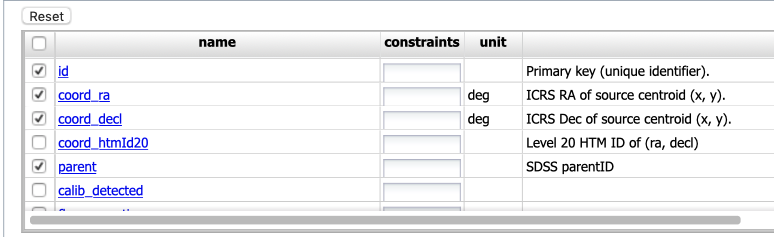
\includegraphics[width=3.12500in]{jira_imgs/244.png}\\

                \vspace{\dp0}
                } \end{minipage} \\ \cdashline{2-3}
                & {\small Test Data} &
                \begin{minipage}[t]{13cm}{\scriptsize
                } \end{minipage} \\ \cdashline{2-3}
                & {\small Expected Result} &
                    \begin{minipage}[t]{13cm}{\scriptsize
                    The column box should be configured to return a minimal useful set of
columns.

                    \vspace{\dp0}
                    } \end{minipage}
                \\ \hdashline


                \multirow{3}{*}{\parbox{1.3cm}{ 2-2
                {\scriptsize from \hyperref[lvv-t851]
                {LVV-T851} } } }

                & {\small Description} &
                \begin{minipage}[t]{13cm}{\scriptsize
                Enter an object name for the portal to resolve. ~We will use NGC 359, a
large elliptical galaxy in the Stripe 82 coverage.\\[2\baselineskip]To
do this, enter the name ``NGC 359'' in the ``Name or Position'' text
input box.\\[2\baselineskip]Leave the other defaults in
place.\\[2\baselineskip]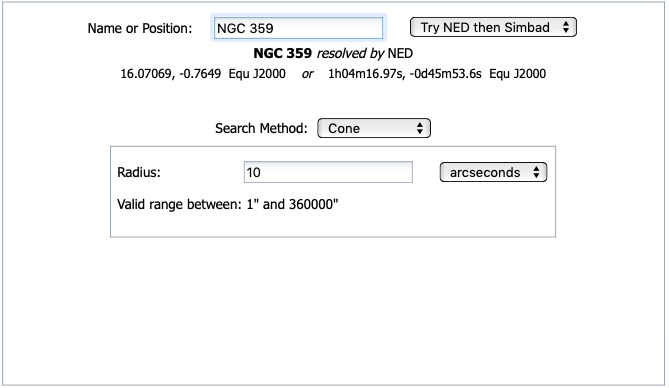
\includegraphics[width=3.12500in]{jira_imgs/245.png}

                \vspace{\dp0}
                } \end{minipage} \\ \cdashline{2-3}
                & {\small Test Data} &
                \begin{minipage}[t]{13cm}{\scriptsize
                } \end{minipage} \\ \cdashline{2-3}
                & {\small Expected Result} &
                    \begin{minipage}[t]{13cm}{\scriptsize
                    There should be a message like ``NGC 359 resolved by NED''. ~The example
coordinates should also changed to the coordinates of NGC 359.

                    \vspace{\dp0}
                    } \end{minipage}
                \\ \hdashline


                \multirow{3}{*}{\parbox{1.3cm}{ 2-3
                {\scriptsize from \hyperref[lvv-t851]
                {LVV-T851} } } }

                & {\small Description} &
                \begin{minipage}[t]{13cm}{\scriptsize
                Submit the query to the portal query engine by clicking the ``Search''
button in the lower left corner of the interface.

                \vspace{\dp0}
                } \end{minipage} \\ \cdashline{2-3}
                & {\small Test Data} &
                \begin{minipage}[t]{13cm}{\scriptsize
                } \end{minipage} \\ \cdashline{2-3}
                & {\small Expected Result} &
                    \begin{minipage}[t]{13cm}{\scriptsize
                    A firefly app with the summary image overlay and catalog widgets side by
side. ~A plot of RA vs. Dec is displayed below the side by side
widgets.\\[2\baselineskip]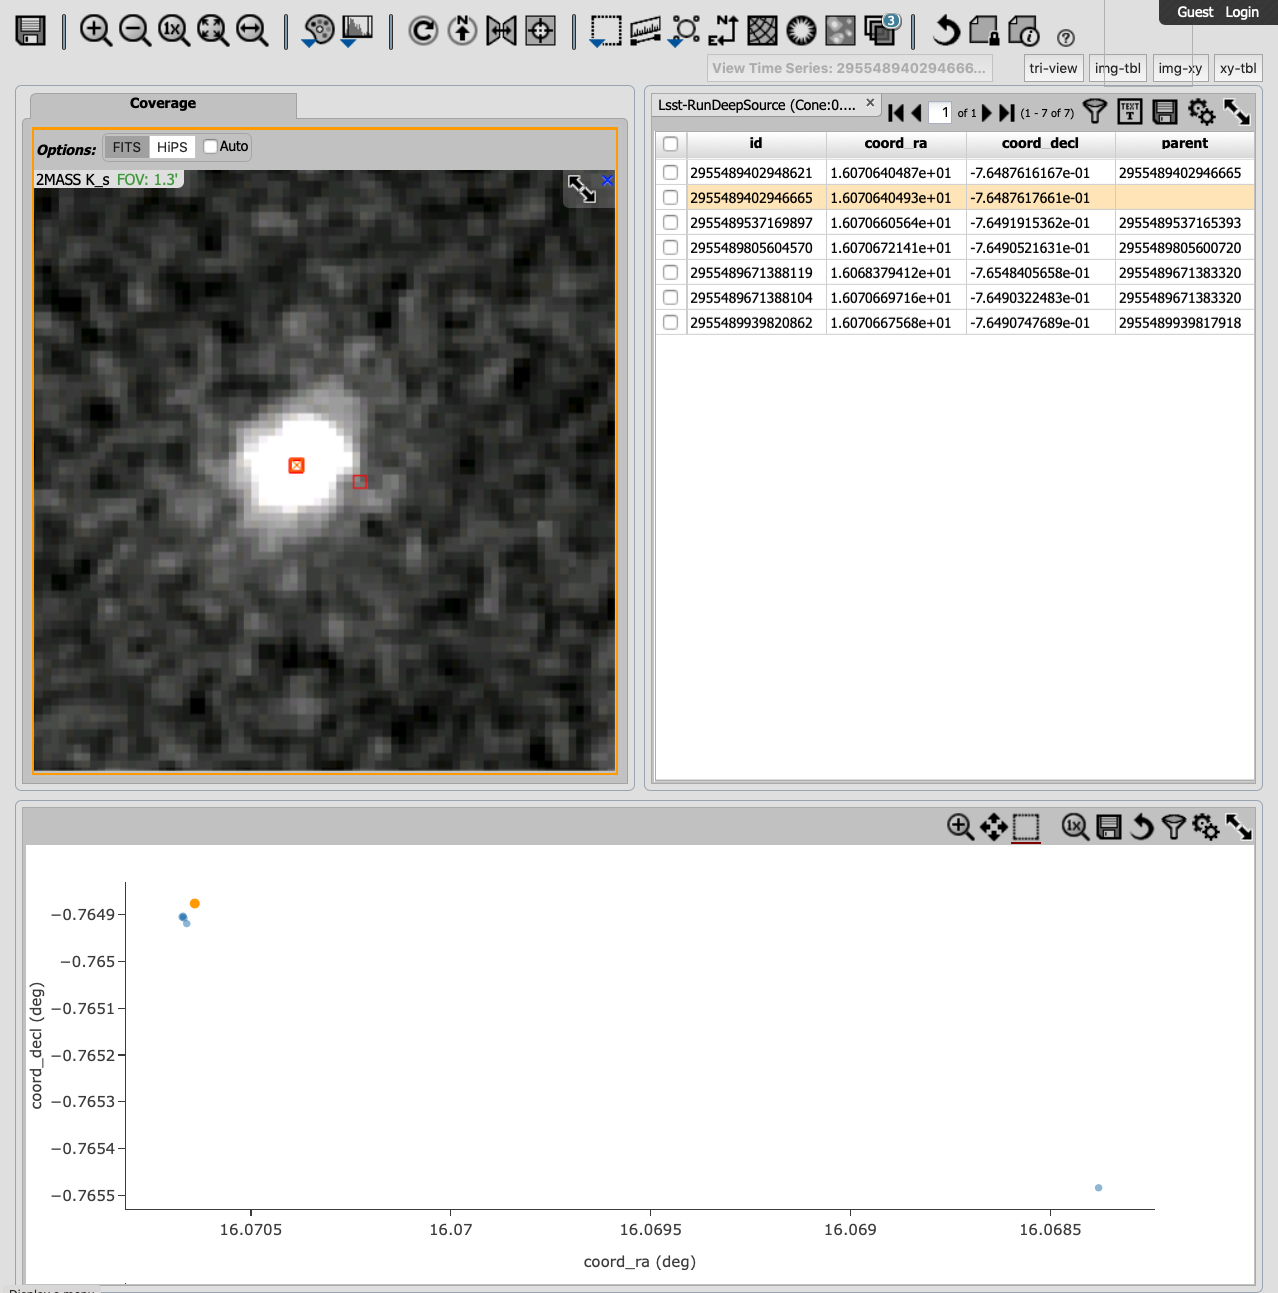
\includegraphics[width=3.12500in]{jira_imgs/246.png}

                    \vspace{\dp0}
                    } \end{minipage}
                \\ \hdashline


        \\ \midrule

            \multirow{3}{*}{ 3 } & Description &
            \begin{minipage}[t]{13cm}{\footnotesize
            Extend the size of the returned table by:\\
1) returning to the query interface by clicking the ``LSST Data'' button
in the upper left of the interface\\
2) update the query by increasing the query radius from 10 to 60
arcseconds\\
3) execute the modified query by clicking the ``Search'' button in the
lower left of the query interface

            \vspace{\dp0}
            } \end{minipage} \\ \cline{2-3}
            & Test Data &
            \begin{minipage}[t]{13cm}{\footnotesize
                No data.
                \vspace{\dp0}
            } \end{minipage} \\ \cline{2-3}
            & Expected Result &
                \begin{minipage}[t]{13cm}{\footnotesize
                An additional table tab of the catalog visualization widget:\\
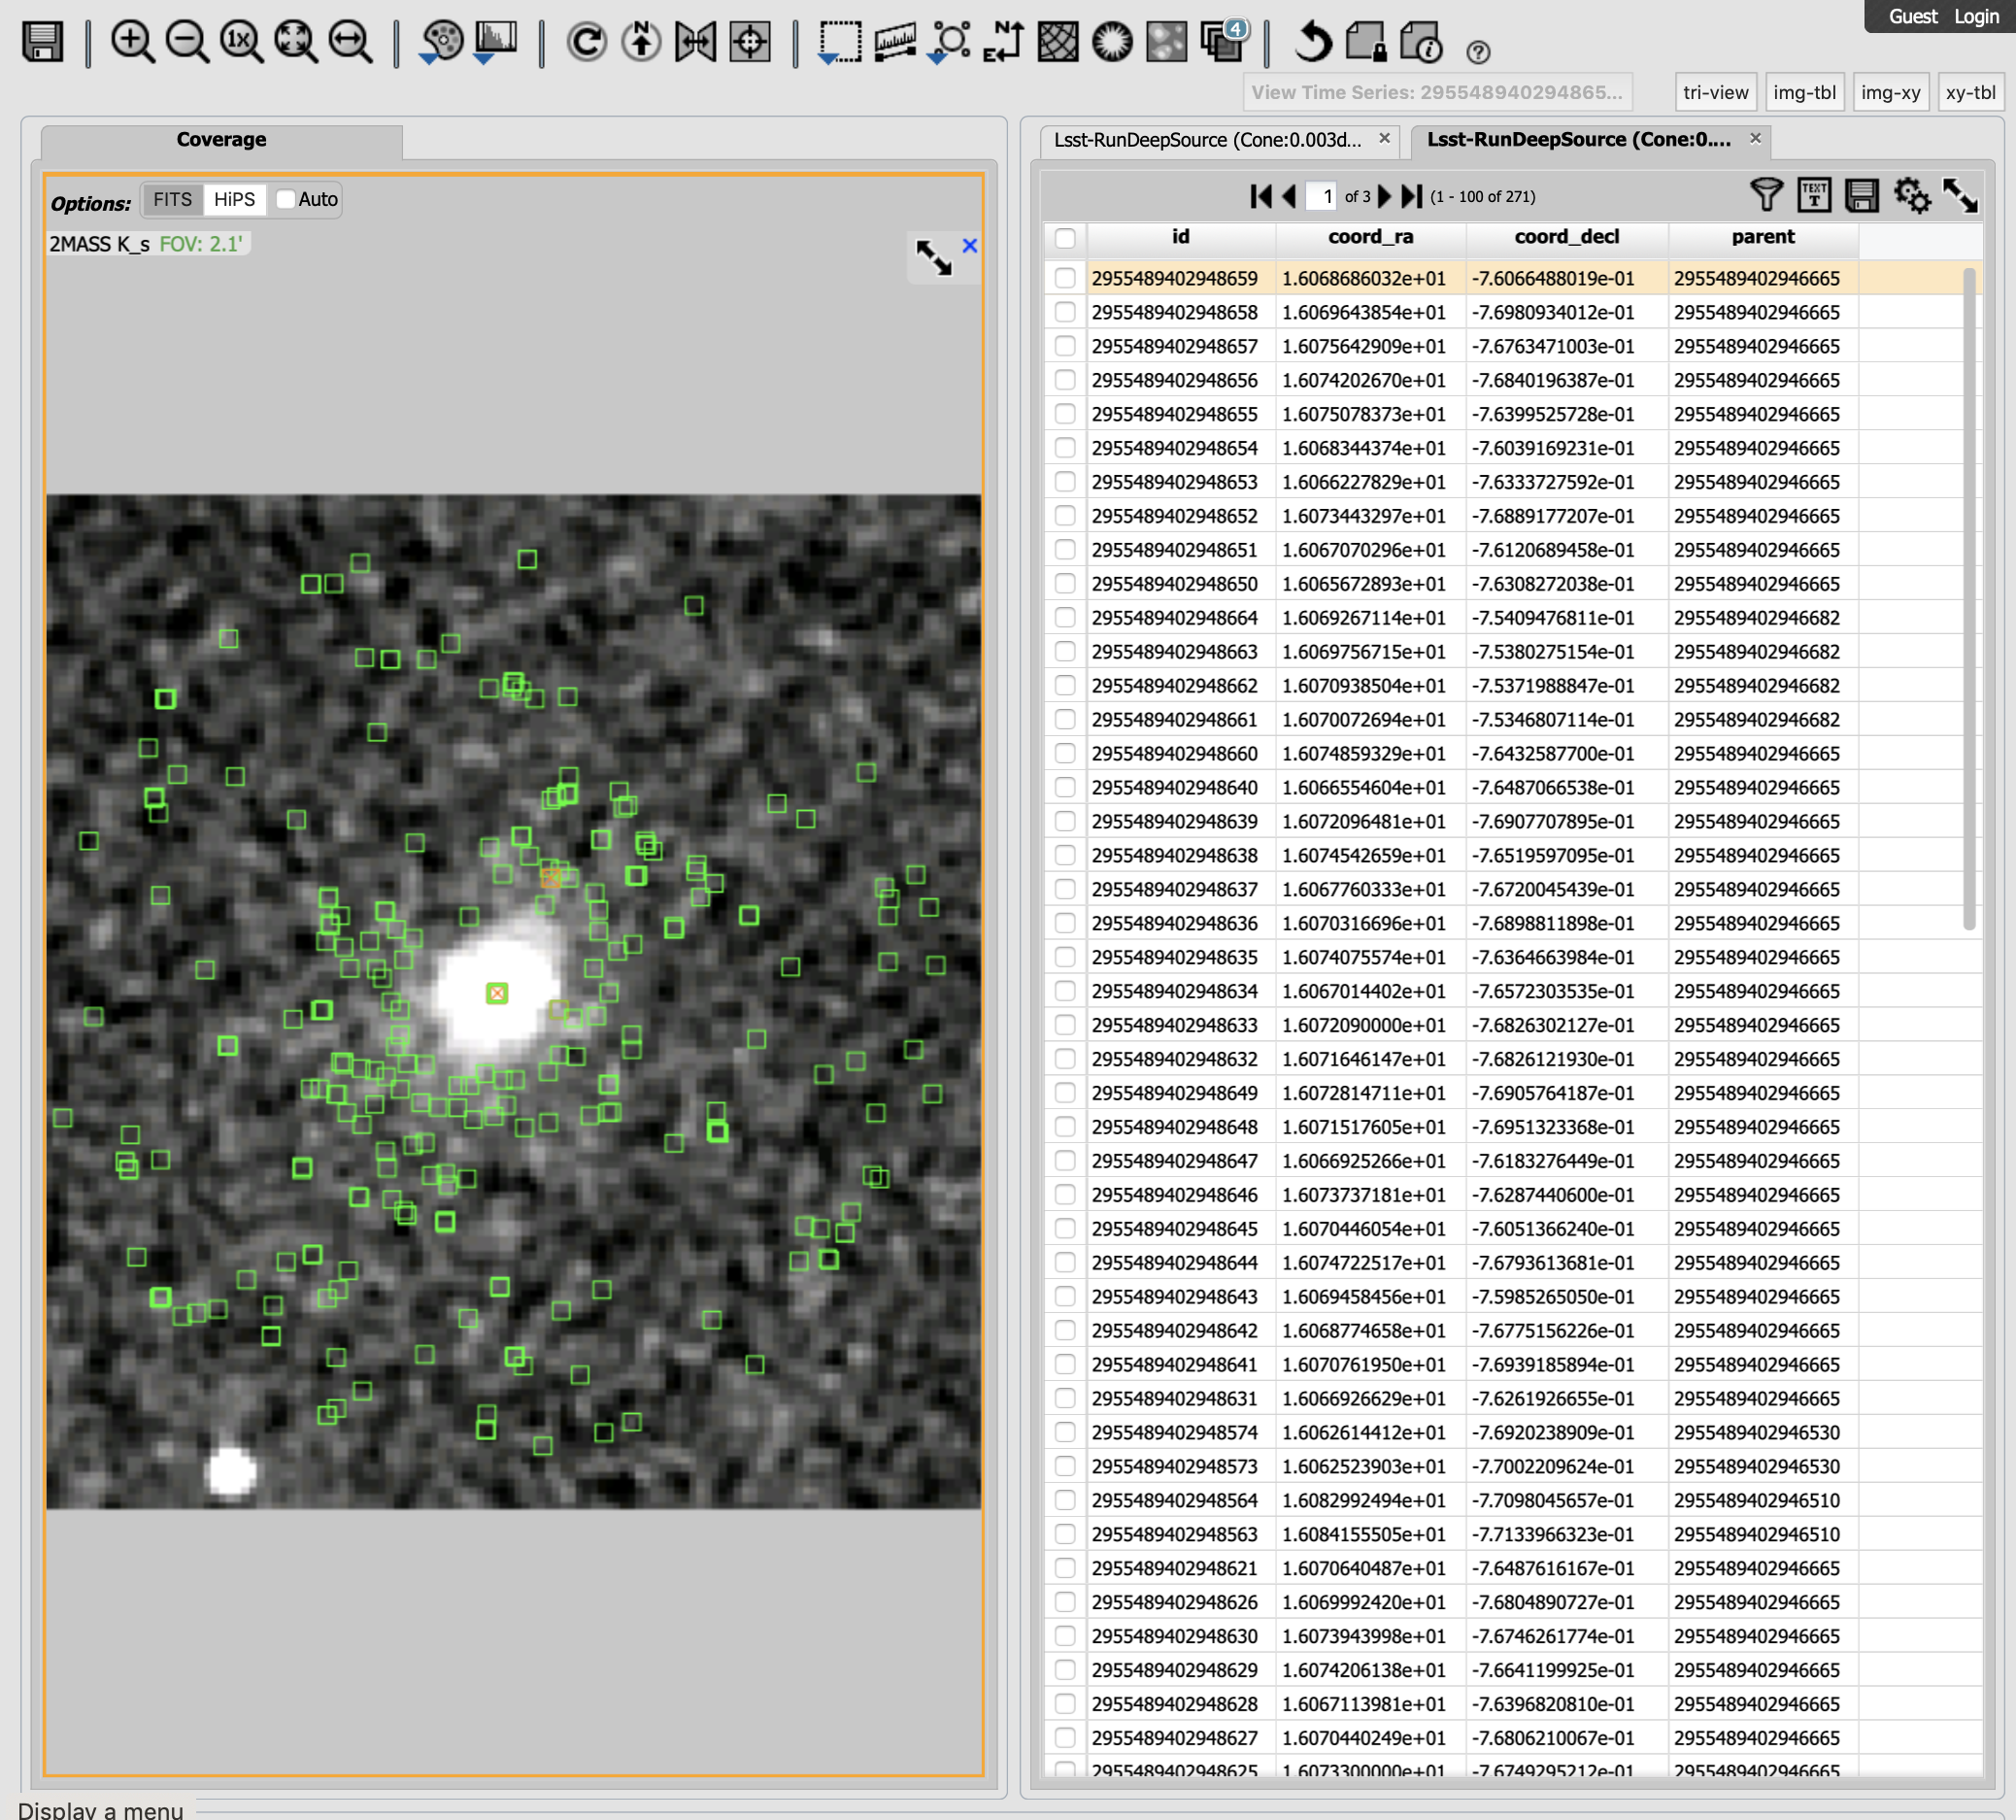
\includegraphics[width=3.12500in]{jira_imgs/251.png}

                \vspace{\dp0}
                } \end{minipage}
        \\ \midrule

            \multirow{3}{*}{ 4 } & Description &
            \begin{minipage}[t]{13cm}{\footnotesize
            Verify the ability to page through the catalog by using the navigation
icons at the upper left of the catalog visualization widget. ~Page
forward to the end of the catalog. ~Use the ``back to beginning''
button.\\

\includegraphics[width=0.25000in]{jira_imgs/253.png}\\

            \vspace{\dp0}
            } \end{minipage} \\ \cline{2-3}
            & Test Data &
            \begin{minipage}[t]{13cm}{\footnotesize
                No data.
                \vspace{\dp0}
            } \end{minipage} \\ \cline{2-3}
            & Expected Result &
                \begin{minipage}[t]{13cm}{\footnotesize
                Expect to be able to page through the catalog and to navigate to the
first or last page from any intervening page.

                \vspace{\dp0}
                } \end{minipage}
        \\ \midrule

                \multirow{3}{*}{\parbox{1.3cm}{ 5-1
                {\scriptsize from \hyperref[lvv-t850]
                {LVV-T850} } } }

                & {\small Description} &
                \begin{minipage}[t]{13cm}{\scriptsize
                Currently, there is no logout mechanism on the portal.\\
This should be updated as the system matures.\\[2\baselineskip]Simply
close the browser window.

                \vspace{\dp0}
                } \end{minipage} \\ \cdashline{2-3}
                & {\small Test Data} &
                \begin{minipage}[t]{13cm}{\scriptsize
                } \end{minipage} \\ \cdashline{2-3}
                & {\small Expected Result} &
                    \begin{minipage}[t]{13cm}{\scriptsize
                    Closed browser window. ~When navigating to the portal endpoint, expect
to execute the steps in LVV-T849.

                    \vspace{\dp0}
                    } \end{minipage}
                \\ \hdashline


        \\ \midrule
    \end{longtable}

\subsection{LVV-T690 - Verify creation and display of X-Y scatter plots}\label{lvv-t690}

\begin{longtable}[]{llllll}
\toprule
Version & Status & Priority & Verification Type & Owner
\\\midrule
1 & Draft & Normal &
Inspection & Jeffrey Carlin
\\\bottomrule
\multicolumn{6}{c}{ Open \href{https://jira.lsstcorp.org/secure/Tests.jspa\#/testCase/LVV-T690}{LVV-T690} in Jira } \\
\end{longtable}

\subsubsection{Verification Elements}
\begin{itemize}
\item \href{https://jira.lsstcorp.org/browse/LVV-9901}{LVV-9901} - DMS-PRTL-REQ-0055-V-01: XY Scatter Plots\_1

\end{itemize}

\subsubsection{Test Items}
Verify that the Portal provides the capability to create and display
2-dimensional X-Y scatter plots from tabular data.


\subsubsection{Predecessors}

\subsubsection{Environment Needs}

\paragraph{Software}

\paragraph{Hardware}

\subsubsection{Input Specification}

\subsubsection{Output Specification}

\subsubsection{Test Procedure}
    \begin{longtable}[]{p{1.3cm}p{2cm}p{13cm}}
    %\toprule
    Step & \multicolumn{2}{@{}l}{Description, Input Data and Expected Result} \\ \toprule
    \endhead

            \multirow{3}{*}{ 1 } & Description &
            \begin{minipage}[t]{13cm}{\footnotesize
            
            \vspace{\dp0}
            } \end{minipage} \\ \cline{2-3}
            & Test Data &
            \begin{minipage}[t]{13cm}{\footnotesize
                No data.
                \vspace{\dp0}
            } \end{minipage} \\ \cline{2-3}
            & Expected Result &
        \\ \midrule
    \end{longtable}

\subsection{LVV-T691 - Verify creation and display of histogram plots}\label{lvv-t691}

\begin{longtable}[]{llllll}
\toprule
Version & Status & Priority & Verification Type & Owner
\\\midrule
1 & Draft & Normal &
Inspection & Jeffrey Carlin
\\\bottomrule
\multicolumn{6}{c}{ Open \href{https://jira.lsstcorp.org/secure/Tests.jspa\#/testCase/LVV-T691}{LVV-T691} in Jira } \\
\end{longtable}

\subsubsection{Verification Elements}
\begin{itemize}
\item \href{https://jira.lsstcorp.org/browse/LVV-9895}{LVV-9895} - DMS-PRTL-REQ-0056-V-01: Histograms\_1

\end{itemize}

\subsubsection{Test Items}
Verify that the Portal provides the capability to create and display
1-dimensional and 2-dimensional histogram plots from tabular data.


\subsubsection{Predecessors}

\subsubsection{Environment Needs}

\paragraph{Software}

\paragraph{Hardware}

\subsubsection{Input Specification}

\subsubsection{Output Specification}

\subsubsection{Test Procedure}
    \begin{longtable}[]{p{1.3cm}p{2cm}p{13cm}}
    %\toprule
    Step & \multicolumn{2}{@{}l}{Description, Input Data and Expected Result} \\ \toprule
    \endhead

            \multirow{3}{*}{ 1 } & Description &
            \begin{minipage}[t]{13cm}{\footnotesize
            
            \vspace{\dp0}
            } \end{minipage} \\ \cline{2-3}
            & Test Data &
            \begin{minipage}[t]{13cm}{\footnotesize
                No data.
                \vspace{\dp0}
            } \end{minipage} \\ \cline{2-3}
            & Expected Result &
        \\ \midrule
    \end{longtable}

\subsection{LVV-T692 - Verify capability to change symbol shapes, sizes, and colors in XY(Z)
scatter plots}\label{lvv-t692}

\begin{longtable}[]{llllll}
\toprule
Version & Status & Priority & Verification Type & Owner
\\\midrule
1 & Draft & Normal &
Inspection & Jeffrey Carlin
\\\bottomrule
\multicolumn{6}{c}{ Open \href{https://jira.lsstcorp.org/secure/Tests.jspa\#/testCase/LVV-T692}{LVV-T692} in Jira } \\
\end{longtable}

\subsubsection{Verification Elements}
\begin{itemize}
\item \href{https://jira.lsstcorp.org/browse/LVV-9900}{LVV-9900} - DMS-PRTL-REQ-0057-V-01: Symbol Size, Shape, and Color Coding in XY(Z)
Scatter Plots\_1

\end{itemize}

\subsubsection{Test Items}
Verify that users can change the shape, size, and color of symbols in
XY(Z) scatter plots to indicate information from additional dimensions
of tabular data.


\subsubsection{Predecessors}

\subsubsection{Environment Needs}

\paragraph{Software}

\paragraph{Hardware}

\subsubsection{Input Specification}

\subsubsection{Output Specification}

\subsubsection{Test Procedure}
    \begin{longtable}[]{p{1.3cm}p{2cm}p{13cm}}
    %\toprule
    Step & \multicolumn{2}{@{}l}{Description, Input Data and Expected Result} \\ \toprule
    \endhead

            \multirow{3}{*}{ 1 } & Description &
            \begin{minipage}[t]{13cm}{\footnotesize
            
            \vspace{\dp0}
            } \end{minipage} \\ \cline{2-3}
            & Test Data &
            \begin{minipage}[t]{13cm}{\footnotesize
                No data.
                \vspace{\dp0}
            } \end{minipage} \\ \cline{2-3}
            & Expected Result &
        \\ \midrule
    \end{longtable}

\subsection{LVV-T693 - Verify visualization of uncertainties in plots}\label{lvv-t693}

\begin{longtable}[]{llllll}
\toprule
Version & Status & Priority & Verification Type & Owner
\\\midrule
1 & Draft & Normal &
Inspection & Jeffrey Carlin
\\\bottomrule
\multicolumn{6}{c}{ Open \href{https://jira.lsstcorp.org/secure/Tests.jspa\#/testCase/LVV-T693}{LVV-T693} in Jira } \\
\end{longtable}

\subsubsection{Verification Elements}
\begin{itemize}
\item \href{https://jira.lsstcorp.org/browse/LVV-9898}{LVV-9898} - DMS-PRTL-REQ-0058-V-01: Plot Quantitative Uncertainties\_1

\end{itemize}

\subsubsection{Test Items}
Verify the capability to represent uncertainties in plots of tabular
data.


\subsubsection{Predecessors}

\subsubsection{Environment Needs}

\paragraph{Software}

\paragraph{Hardware}

\subsubsection{Input Specification}

\subsubsection{Output Specification}

\subsubsection{Test Procedure}
    \begin{longtable}[]{p{1.3cm}p{2cm}p{13cm}}
    %\toprule
    Step & \multicolumn{2}{@{}l}{Description, Input Data and Expected Result} \\ \toprule
    \endhead

            \multirow{3}{*}{ 1 } & Description &
            \begin{minipage}[t]{13cm}{\footnotesize
            
            \vspace{\dp0}
            } \end{minipage} \\ \cline{2-3}
            & Test Data &
            \begin{minipage}[t]{13cm}{\footnotesize
                No data.
                \vspace{\dp0}
            } \end{minipage} \\ \cline{2-3}
            & Expected Result &
        \\ \midrule
    \end{longtable}

\subsection{LVV-T694 - Verify visualization of asymmetric uncertainties}\label{lvv-t694}

\begin{longtable}[]{llllll}
\toprule
Version & Status & Priority & Verification Type & Owner
\\\midrule
1 & Draft & Normal &
Inspection & Jeffrey Carlin
\\\bottomrule
\multicolumn{6}{c}{ Open \href{https://jira.lsstcorp.org/secure/Tests.jspa\#/testCase/LVV-T694}{LVV-T694} in Jira } \\
\end{longtable}

\subsubsection{Verification Elements}
\begin{itemize}
\item \href{https://jira.lsstcorp.org/browse/LVV-9897}{LVV-9897} - DMS-PRTL-REQ-0059-V-01: Plot Asymmetric Quantitative Uncertainties\_1

\end{itemize}

\subsubsection{Test Items}
Verify that the Portal aspect can display uncertainties that are
asymmetric (i.e., differ in the positive and negative directions).~


\subsubsection{Predecessors}

\subsubsection{Environment Needs}

\paragraph{Software}

\paragraph{Hardware}

\subsubsection{Input Specification}

\subsubsection{Output Specification}

\subsubsection{Test Procedure}
    \begin{longtable}[]{p{1.3cm}p{2cm}p{13cm}}
    %\toprule
    Step & \multicolumn{2}{@{}l}{Description, Input Data and Expected Result} \\ \toprule
    \endhead

            \multirow{3}{*}{ 1 } & Description &
            \begin{minipage}[t]{13cm}{\footnotesize
            
            \vspace{\dp0}
            } \end{minipage} \\ \cline{2-3}
            & Test Data &
            \begin{minipage}[t]{13cm}{\footnotesize
                No data.
                \vspace{\dp0}
            } \end{minipage} \\ \cline{2-3}
            & Expected Result &
        \\ \midrule
    \end{longtable}

\subsection{LVV-T695 - Verify visualization of upper and lower limits in plots}\label{lvv-t695}

\begin{longtable}[]{llllll}
\toprule
Version & Status & Priority & Verification Type & Owner
\\\midrule
1 & Draft & Normal &
Inspection & Jeffrey Carlin
\\\bottomrule
\multicolumn{6}{c}{ Open \href{https://jira.lsstcorp.org/secure/Tests.jspa\#/testCase/LVV-T695}{LVV-T695} in Jira } \\
\end{longtable}

\subsubsection{Verification Elements}
\begin{itemize}
\item \href{https://jira.lsstcorp.org/browse/LVV-9899}{LVV-9899} - DMS-PRTL-REQ-0060-V-01: Plot Upper and Lower Quantitative Limits\_1

\end{itemize}

\subsubsection{Test Items}
Verify that the Portal is capable of displaying quantities that
represent upper or lower limits (provided, for example, for
non-detections).


\subsubsection{Predecessors}

\subsubsection{Environment Needs}

\paragraph{Software}

\paragraph{Hardware}

\subsubsection{Input Specification}

\subsubsection{Output Specification}

\subsubsection{Test Procedure}
    \begin{longtable}[]{p{1.3cm}p{2cm}p{13cm}}
    %\toprule
    Step & \multicolumn{2}{@{}l}{Description, Input Data and Expected Result} \\ \toprule
    \endhead

            \multirow{3}{*}{ 1 } & Description &
            \begin{minipage}[t]{13cm}{\footnotesize
            
            \vspace{\dp0}
            } \end{minipage} \\ \cline{2-3}
            & Test Data &
            \begin{minipage}[t]{13cm}{\footnotesize
                No data.
                \vspace{\dp0}
            } \end{minipage} \\ \cline{2-3}
            & Expected Result &
        \\ \midrule
    \end{longtable}

\subsection{LVV-T696 - Verify visualization of multiple XY plots on the same display}\label{lvv-t696}

\begin{longtable}[]{llllll}
\toprule
Version & Status & Priority & Verification Type & Owner
\\\midrule
1 & Draft & Normal &
Inspection & Jeffrey Carlin
\\\bottomrule
\multicolumn{6}{c}{ Open \href{https://jira.lsstcorp.org/secure/Tests.jspa\#/testCase/LVV-T696}{LVV-T696} in Jira } \\
\end{longtable}

\subsubsection{Verification Elements}
\begin{itemize}
\item \href{https://jira.lsstcorp.org/browse/LVV-9896}{LVV-9896} - DMS-PRTL-REQ-0061-V-01: Multiple XY-Plots on the Same Display\_1

\end{itemize}

\subsubsection{Test Items}
Verify that the Portal provides the capability to display multiple XY
plots on a single display canvas.


\subsubsection{Predecessors}

\subsubsection{Environment Needs}

\paragraph{Software}

\paragraph{Hardware}

\subsubsection{Input Specification}

\subsubsection{Output Specification}

\subsubsection{Test Procedure}
    \begin{longtable}[]{p{1.3cm}p{2cm}p{13cm}}
    %\toprule
    Step & \multicolumn{2}{@{}l}{Description, Input Data and Expected Result} \\ \toprule
    \endhead

            \multirow{3}{*}{ 1 } & Description &
            \begin{minipage}[t]{13cm}{\footnotesize
            
            \vspace{\dp0}
            } \end{minipage} \\ \cline{2-3}
            & Test Data &
            \begin{minipage}[t]{13cm}{\footnotesize
                No data.
                \vspace{\dp0}
            } \end{minipage} \\ \cline{2-3}
            & Expected Result &
        \\ \midrule
    \end{longtable}

\subsection{LVV-T697 - Verify display of raft and full focal-plane single-visit images}\label{lvv-t697}

\begin{longtable}[]{llllll}
\toprule
Version & Status & Priority & Verification Type & Owner
\\\midrule
1 & Draft & Normal &
Inspection & Jeffrey Carlin
\\\bottomrule
\multicolumn{6}{c}{ Open \href{https://jira.lsstcorp.org/secure/Tests.jspa\#/testCase/LVV-T697}{LVV-T697} in Jira } \\
\end{longtable}

\subsubsection{Verification Elements}
\begin{itemize}
\item \href{https://jira.lsstcorp.org/browse/LVV-9906}{LVV-9906} - DMS-PRTL-REQ-0063-V-01: Display Raft- and Focal-Plane-Level Single-Visit
Image Data\_1

\end{itemize}

\subsubsection{Test Items}
Verify that the Portal aspect has the ability to generate a single-visit
image display of a raft and full focal-plane image.


\subsubsection{Predecessors}

\subsubsection{Environment Needs}

\paragraph{Software}

\paragraph{Hardware}

\subsubsection{Input Specification}

\subsubsection{Output Specification}

\subsubsection{Test Procedure}
    \begin{longtable}[]{p{1.3cm}p{2cm}p{13cm}}
    %\toprule
    Step & \multicolumn{2}{@{}l}{Description, Input Data and Expected Result} \\ \toprule
    \endhead

            \multirow{3}{*}{ 1 } & Description &
            \begin{minipage}[t]{13cm}{\footnotesize
            
            \vspace{\dp0}
            } \end{minipage} \\ \cline{2-3}
            & Test Data &
            \begin{minipage}[t]{13cm}{\footnotesize
                No data.
                \vspace{\dp0}
            } \end{minipage} \\ \cline{2-3}
            & Expected Result &
        \\ \midrule
    \end{longtable}

\subsection{LVV-T698 - Verify display of cutout from single-visit image}\label{lvv-t698}

\begin{longtable}[]{llllll}
\toprule
Version & Status & Priority & Verification Type & Owner
\\\midrule
1 & Draft & Normal &
Inspection & Jeffrey Carlin
\\\bottomrule
\multicolumn{6}{c}{ Open \href{https://jira.lsstcorp.org/secure/Tests.jspa\#/testCase/LVV-T698}{LVV-T698} in Jira } \\
\end{longtable}

\subsubsection{Verification Elements}
\begin{itemize}
\item \href{https://jira.lsstcorp.org/browse/LVV-9907}{LVV-9907} - DMS-PRTL-REQ-0064-V-01: Display Single Visit Image Cut-Out\_1

\end{itemize}

\subsubsection{Test Items}
Verify that the Portal is capable of displaying a cutout from a
single-visit image.


\subsubsection{Predecessors}

\subsubsection{Environment Needs}

\paragraph{Software}

\paragraph{Hardware}

\subsubsection{Input Specification}

\subsubsection{Output Specification}

\subsubsection{Test Procedure}
    \begin{longtable}[]{p{1.3cm}p{2cm}p{13cm}}
    %\toprule
    Step & \multicolumn{2}{@{}l}{Description, Input Data and Expected Result} \\ \toprule
    \endhead

            \multirow{3}{*}{ 1 } & Description &
            \begin{minipage}[t]{13cm}{\footnotesize
            
            \vspace{\dp0}
            } \end{minipage} \\ \cline{2-3}
            & Test Data &
            \begin{minipage}[t]{13cm}{\footnotesize
                No data.
                \vspace{\dp0}
            } \end{minipage} \\ \cline{2-3}
            & Expected Result &
        \\ \midrule
    \end{longtable}

\subsection{LVV-T699 - Verify display of native coadd images}\label{lvv-t699}

\begin{longtable}[]{llllll}
\toprule
Version & Status & Priority & Verification Type & Owner
\\\midrule
1 & Draft & Normal &
Inspection & Jeffrey Carlin
\\\bottomrule
\multicolumn{6}{c}{ Open \href{https://jira.lsstcorp.org/secure/Tests.jspa\#/testCase/LVV-T699}{LVV-T699} in Jira } \\
\end{longtable}

\subsubsection{Verification Elements}
\begin{itemize}
\item \href{https://jira.lsstcorp.org/browse/LVV-9904}{LVV-9904} - DMS-PRTL-REQ-0065-V-01: Display Native Coadded Image Data Products\_1

\end{itemize}

\subsubsection{Test Items}
Verify that the Portal can display native coadd image products (i.e.,
patch-level images).


\subsubsection{Predecessors}

\subsubsection{Environment Needs}

\paragraph{Software}

\paragraph{Hardware}

\subsubsection{Input Specification}

\subsubsection{Output Specification}

\subsubsection{Test Procedure}
    \begin{longtable}[]{p{1.3cm}p{2cm}p{13cm}}
    %\toprule
    Step & \multicolumn{2}{@{}l}{Description, Input Data and Expected Result} \\ \toprule
    \endhead

            \multirow{3}{*}{ 1 } & Description &
            \begin{minipage}[t]{13cm}{\footnotesize
            
            \vspace{\dp0}
            } \end{minipage} \\ \cline{2-3}
            & Test Data &
            \begin{minipage}[t]{13cm}{\footnotesize
                No data.
                \vspace{\dp0}
            } \end{minipage} \\ \cline{2-3}
            & Expected Result &
        \\ \midrule
    \end{longtable}

\subsection{LVV-T700 - Verify display of coadd cutouts and mosaics}\label{lvv-t700}

\begin{longtable}[]{llllll}
\toprule
Version & Status & Priority & Verification Type & Owner
\\\midrule
1 & Draft & Normal &
Inspection & Jeffrey Carlin
\\\bottomrule
\multicolumn{6}{c}{ Open \href{https://jira.lsstcorp.org/secure/Tests.jspa\#/testCase/LVV-T700}{LVV-T700} in Jira } \\
\end{longtable}

\subsubsection{Verification Elements}
\begin{itemize}
\item \href{https://jira.lsstcorp.org/browse/LVV-9903}{LVV-9903} - DMS-PRTL-REQ-0066-V-01: Display Coadded Image Cutouts / Mosaics\_1

\end{itemize}

\subsubsection{Test Items}
Verify that the Portal aspect has the capability to display cutout or
mosaic images created from coadds.


\subsubsection{Predecessors}

\subsubsection{Environment Needs}

\paragraph{Software}

\paragraph{Hardware}

\subsubsection{Input Specification}

\subsubsection{Output Specification}

\subsubsection{Test Procedure}
    \begin{longtable}[]{p{1.3cm}p{2cm}p{13cm}}
    %\toprule
    Step & \multicolumn{2}{@{}l}{Description, Input Data and Expected Result} \\ \toprule
    \endhead

            \multirow{3}{*}{ 1 } & Description &
            \begin{minipage}[t]{13cm}{\footnotesize
            
            \vspace{\dp0}
            } \end{minipage} \\ \cline{2-3}
            & Test Data &
            \begin{minipage}[t]{13cm}{\footnotesize
                No data.
                \vspace{\dp0}
            } \end{minipage} \\ \cline{2-3}
            & Expected Result &
        \\ \midrule
    \end{longtable}

\subsection{LVV-T701 - Verify display of calibration images}\label{lvv-t701}

\begin{longtable}[]{llllll}
\toprule
Version & Status & Priority & Verification Type & Owner
\\\midrule
1 & Draft & Normal &
Inspection & Jeffrey Carlin
\\\bottomrule
\multicolumn{6}{c}{ Open \href{https://jira.lsstcorp.org/secure/Tests.jspa\#/testCase/LVV-T701}{LVV-T701} in Jira } \\
\end{longtable}

\subsubsection{Verification Elements}
\begin{itemize}
\item \href{https://jira.lsstcorp.org/browse/LVV-9902}{LVV-9902} - DMS-PRTL-REQ-0067-V-01: Display Calibration Image Data Products\_1

\end{itemize}

\subsubsection{Test Items}
Verify that the Portal is capable of displaying calibration image data
products, including synthetic flats, bias frames, etc.


\subsubsection{Predecessors}

\subsubsection{Environment Needs}

\paragraph{Software}

\paragraph{Hardware}

\subsubsection{Input Specification}

\subsubsection{Output Specification}

\subsubsection{Test Procedure}
    \begin{longtable}[]{p{1.3cm}p{2cm}p{13cm}}
    %\toprule
    Step & \multicolumn{2}{@{}l}{Description, Input Data and Expected Result} \\ \toprule
    \endhead

            \multirow{3}{*}{ 1 } & Description &
            \begin{minipage}[t]{13cm}{\footnotesize
            
            \vspace{\dp0}
            } \end{minipage} \\ \cline{2-3}
            & Test Data &
            \begin{minipage}[t]{13cm}{\footnotesize
                No data.
                \vspace{\dp0}
            } \end{minipage} \\ \cline{2-3}
            & Expected Result &
        \\ \midrule
    \end{longtable}

\subsection{LVV-T702 - Verify display of user-provided images}\label{lvv-t702}

\begin{longtable}[]{llllll}
\toprule
Version & Status & Priority & Verification Type & Owner
\\\midrule
1 & Draft & Normal &
Inspection & Jeffrey Carlin
\\\bottomrule
\multicolumn{6}{c}{ Open \href{https://jira.lsstcorp.org/secure/Tests.jspa\#/testCase/LVV-T702}{LVV-T702} in Jira } \\
\end{longtable}

\subsubsection{Verification Elements}
\begin{itemize}
\item \href{https://jira.lsstcorp.org/browse/LVV-9908}{LVV-9908} - DMS-PRTL-REQ-0068-V-01: Display User-provided Images\_1

\end{itemize}

\subsubsection{Test Items}
Verify that the Portal has the capability of displaying user-provided
images in widely-used astronomical data formats, and properly interprets
commonly-used WCS specifications from the image headers. This includes
FITS format, and may be extended to others.~


\subsubsection{Predecessors}

\subsubsection{Environment Needs}

\paragraph{Software}

\paragraph{Hardware}

\subsubsection{Input Specification}

\subsubsection{Output Specification}

\subsubsection{Test Procedure}
    \begin{longtable}[]{p{1.3cm}p{2cm}p{13cm}}
    %\toprule
    Step & \multicolumn{2}{@{}l}{Description, Input Data and Expected Result} \\ \toprule
    \endhead

            \multirow{3}{*}{ 1 } & Description &
            \begin{minipage}[t]{13cm}{\footnotesize
            
            \vspace{\dp0}
            } \end{minipage} \\ \cline{2-3}
            & Test Data &
            \begin{minipage}[t]{13cm}{\footnotesize
                No data.
                \vspace{\dp0}
            } \end{minipage} \\ \cline{2-3}
            & Expected Result &
        \\ \midrule
    \end{longtable}

\subsection{LVV-T703 - Verify display of image property sheet}\label{lvv-t703}

\begin{longtable}[]{llllll}
\toprule
Version & Status & Priority & Verification Type & Owner
\\\midrule
1 & Draft & Normal &
Inspection & Jeffrey Carlin
\\\bottomrule
\multicolumn{6}{c}{ Open \href{https://jira.lsstcorp.org/secure/Tests.jspa\#/testCase/LVV-T703}{LVV-T703} in Jira } \\
\end{longtable}

\subsubsection{Verification Elements}
\begin{itemize}
\item \href{https://jira.lsstcorp.org/browse/LVV-9909}{LVV-9909} - DMS-PRTL-REQ-0069-V-01: Image Property Sheet\_1

\end{itemize}

\subsubsection{Test Items}
Verify that the Portal has the ability to display a property sheet for
an image data product or user-provided image, displaying image format
and other header data.


\subsubsection{Predecessors}

\subsubsection{Environment Needs}

\paragraph{Software}

\paragraph{Hardware}

\subsubsection{Input Specification}

\subsubsection{Output Specification}

\subsubsection{Test Procedure}
    \begin{longtable}[]{p{1.3cm}p{2cm}p{13cm}}
    %\toprule
    Step & \multicolumn{2}{@{}l}{Description, Input Data and Expected Result} \\ \toprule
    \endhead

            \multirow{3}{*}{ 1 } & Description &
            \begin{minipage}[t]{13cm}{\footnotesize
            
            \vspace{\dp0}
            } \end{minipage} \\ \cline{2-3}
            & Test Data &
            \begin{minipage}[t]{13cm}{\footnotesize
                No data.
                \vspace{\dp0}
            } \end{minipage} \\ \cline{2-3}
            & Expected Result &
        \\ \midrule
    \end{longtable}

\subsection{LVV-T704 - Verify that coordinate display tools are provided for images}\label{lvv-t704}

\begin{longtable}[]{llllll}
\toprule
Version & Status & Priority & Verification Type & Owner
\\\midrule
1 & Draft & Normal &
Inspection & Jeffrey Carlin
\\\bottomrule
\multicolumn{6}{c}{ Open \href{https://jira.lsstcorp.org/secure/Tests.jspa\#/testCase/LVV-T704}{LVV-T704} in Jira } \\
\end{longtable}

\subsubsection{Verification Elements}
\begin{itemize}
\item \href{https://jira.lsstcorp.org/browse/LVV-9914}{LVV-9914} - DMS-PRTL-REQ-0070-V-01: Provide Coordinate Display Tools for Images\_1

\end{itemize}

\subsubsection{Test Items}
Verify that the Portal provides all the capabilities in the Coordinate
Display Tools section in \citeds{LDM-554} for image displays. Specific
capabilities will depend on the availability of WCS information for an
image.


\subsubsection{Predecessors}

\subsubsection{Environment Needs}

\paragraph{Software}

\paragraph{Hardware}

\subsubsection{Input Specification}

\subsubsection{Output Specification}

\subsubsection{Test Procedure}
    \begin{longtable}[]{p{1.3cm}p{2cm}p{13cm}}
    %\toprule
    Step & \multicolumn{2}{@{}l}{Description, Input Data and Expected Result} \\ \toprule
    \endhead

            \multirow{3}{*}{ 1 } & Description &
            \begin{minipage}[t]{13cm}{\footnotesize
            
            \vspace{\dp0}
            } \end{minipage} \\ \cline{2-3}
            & Test Data &
            \begin{minipage}[t]{13cm}{\footnotesize
                No data.
                \vspace{\dp0}
            } \end{minipage} \\ \cline{2-3}
            & Expected Result &
        \\ \midrule
    \end{longtable}

\subsection{LVV-T705 - Verify image pixel content display}\label{lvv-t705}

\begin{longtable}[]{llllll}
\toprule
Version & Status & Priority & Verification Type & Owner
\\\midrule
1 & Draft & Normal &
Inspection & Jeffrey Carlin
\\\bottomrule
\multicolumn{6}{c}{ Open \href{https://jira.lsstcorp.org/secure/Tests.jspa\#/testCase/LVV-T705}{LVV-T705} in Jira } \\
\end{longtable}

\subsubsection{Verification Elements}
\begin{itemize}
\item \href{https://jira.lsstcorp.org/browse/LVV-9911}{LVV-9911} - DMS-PRTL-REQ-0071-V-01: Image Pixel Content Display\_1

\end{itemize}

\subsubsection{Test Items}
Verify that the Portal provides the capability to inspect the pixel
contents of an image at the cursor position.


\subsubsection{Predecessors}

\subsubsection{Environment Needs}

\paragraph{Software}

\paragraph{Hardware}

\subsubsection{Input Specification}

\subsubsection{Output Specification}

\subsubsection{Test Procedure}
    \begin{longtable}[]{p{1.3cm}p{2cm}p{13cm}}
    %\toprule
    Step & \multicolumn{2}{@{}l}{Description, Input Data and Expected Result} \\ \toprule
    \endhead

            \multirow{3}{*}{ 1 } & Description &
            \begin{minipage}[t]{13cm}{\footnotesize
            
            \vspace{\dp0}
            } \end{minipage} \\ \cline{2-3}
            & Test Data &
            \begin{minipage}[t]{13cm}{\footnotesize
                No data.
                \vspace{\dp0}
            } \end{minipage} \\ \cline{2-3}
            & Expected Result &
        \\ \midrule
    \end{longtable}

\subsection{LVV-T706 - Verify spatial manipulation of images}\label{lvv-t706}

\begin{longtable}[]{llllll}
\toprule
Version & Status & Priority & Verification Type & Owner
\\\midrule
1 & Draft & Normal &
Inspection & Jeffrey Carlin
\\\bottomrule
\multicolumn{6}{c}{ Open \href{https://jira.lsstcorp.org/secure/Tests.jspa\#/testCase/LVV-T706}{LVV-T706} in Jira } \\
\end{longtable}

\subsubsection{Verification Elements}
\begin{itemize}
\item \href{https://jira.lsstcorp.org/browse/LVV-9912}{LVV-9912} - DMS-PRTL-REQ-0072-V-01: Image Spatial Manipulation\_1

\end{itemize}

\subsubsection{Test Items}
Verify that the Portal allows users to spatially manipulate displayed
images, including resizing, rescaling, reprojecting, zooming, and
cropping.


\subsubsection{Predecessors}

\subsubsection{Environment Needs}

\paragraph{Software}

\paragraph{Hardware}

\subsubsection{Input Specification}

\subsubsection{Output Specification}

\subsubsection{Test Procedure}
    \begin{longtable}[]{p{1.3cm}p{2cm}p{13cm}}
    %\toprule
    Step & \multicolumn{2}{@{}l}{Description, Input Data and Expected Result} \\ \toprule
    \endhead

            \multirow{3}{*}{ 1 } & Description &
            \begin{minipage}[t]{13cm}{\footnotesize
            
            \vspace{\dp0}
            } \end{minipage} \\ \cline{2-3}
            & Test Data &
            \begin{minipage}[t]{13cm}{\footnotesize
                No data.
                \vspace{\dp0}
            } \end{minipage} \\ \cline{2-3}
            & Expected Result &
        \\ \midrule
    \end{longtable}

\subsection{LVV-T707 - Verify multi-image scaling and alignment}\label{lvv-t707}

\begin{longtable}[]{llllll}
\toprule
Version & Status & Priority & Verification Type & Owner
\\\midrule
1 & Draft & Normal &
Inspection & Jeffrey Carlin
\\\bottomrule
\multicolumn{6}{c}{ Open \href{https://jira.lsstcorp.org/secure/Tests.jspa\#/testCase/LVV-T707}{LVV-T707} in Jira } \\
\end{longtable}

\subsubsection{Verification Elements}
\begin{itemize}
\item \href{https://jira.lsstcorp.org/browse/LVV-9913}{LVV-9913} - DMS-PRTL-REQ-0073-V-01: Multi-Image Scaling and Aligning\_1

\end{itemize}

\subsubsection{Test Items}
Verify that the Portal has the capability to display multiple images on
a common astrophysical coordinate scale, aligned on the screen in a
common orientation.


\subsubsection{Predecessors}

\subsubsection{Environment Needs}

\paragraph{Software}

\paragraph{Hardware}

\subsubsection{Input Specification}

\subsubsection{Output Specification}

\subsubsection{Test Procedure}
    \begin{longtable}[]{p{1.3cm}p{2cm}p{13cm}}
    %\toprule
    Step & \multicolumn{2}{@{}l}{Description, Input Data and Expected Result} \\ \toprule
    \endhead

            \multirow{3}{*}{ 1 } & Description &
            \begin{minipage}[t]{13cm}{\footnotesize
            
            \vspace{\dp0}
            } \end{minipage} \\ \cline{2-3}
            & Test Data &
            \begin{minipage}[t]{13cm}{\footnotesize
                No data.
                \vspace{\dp0}
            } \end{minipage} \\ \cline{2-3}
            & Expected Result &
        \\ \midrule
    \end{longtable}

\subsection{LVV-T708 - Verify manipulation of image appearance}\label{lvv-t708}

\begin{longtable}[]{llllll}
\toprule
Version & Status & Priority & Verification Type & Owner
\\\midrule
1 & Draft & Normal &
Inspection & Jeffrey Carlin
\\\bottomrule
\multicolumn{6}{c}{ Open \href{https://jira.lsstcorp.org/secure/Tests.jspa\#/testCase/LVV-T708}{LVV-T708} in Jira } \\
\end{longtable}

\subsubsection{Verification Elements}
\begin{itemize}
\item \href{https://jira.lsstcorp.org/browse/LVV-9910}{LVV-9910} - DMS-PRTL-REQ-0074-V-01: Image Appearance Manipulation\_1

\end{itemize}

\subsubsection{Test Items}
Verify that the Portal enables users to manipulate the appearance of
displayed images, including changing the stretch, color table, or
displayed data range.


\subsubsection{Predecessors}

\subsubsection{Environment Needs}

\paragraph{Software}

\paragraph{Hardware}

\subsubsection{Input Specification}

\subsubsection{Output Specification}

\subsubsection{Test Procedure}
    \begin{longtable}[]{p{1.3cm}p{2cm}p{13cm}}
    %\toprule
    Step & \multicolumn{2}{@{}l}{Description, Input Data and Expected Result} \\ \toprule
    \endhead

            \multirow{3}{*}{ 1 } & Description &
            \begin{minipage}[t]{13cm}{\footnotesize
            
            \vspace{\dp0}
            } \end{minipage} \\ \cline{2-3}
            & Test Data &
            \begin{minipage}[t]{13cm}{\footnotesize
                No data.
                \vspace{\dp0}
            } \end{minipage} \\ \cline{2-3}
            & Expected Result &
        \\ \midrule
    \end{longtable}

\subsection{LVV-T709 - Verify display of image mask and variance overlays}\label{lvv-t709}

\begin{longtable}[]{llllll}
\toprule
Version & Status & Priority & Verification Type & Owner
\\\midrule
1 & Draft & Normal &
Inspection & Jeffrey Carlin
\\\bottomrule
\multicolumn{6}{c}{ Open \href{https://jira.lsstcorp.org/secure/Tests.jspa\#/testCase/LVV-T709}{LVV-T709} in Jira } \\
\end{longtable}

\subsubsection{Verification Elements}
\begin{itemize}
\item \href{https://jira.lsstcorp.org/browse/LVV-9915}{LVV-9915} - DMS-PRTL-REQ-0075-V-01: Image Mask and Variance Overlays\_1

\end{itemize}

\subsubsection{Test Items}
Verify that the Portal enables overlaying pixel-based data on top of
already displayed images, including image masks (bit planes) and
variance data.


\subsubsection{Predecessors}

\subsubsection{Environment Needs}

\paragraph{Software}

\paragraph{Hardware}

\subsubsection{Input Specification}

\subsubsection{Output Specification}

\subsubsection{Test Procedure}
    \begin{longtable}[]{p{1.3cm}p{2cm}p{13cm}}
    %\toprule
    Step & \multicolumn{2}{@{}l}{Description, Input Data and Expected Result} \\ \toprule
    \endhead

            \multirow{3}{*}{ 1 } & Description &
            \begin{minipage}[t]{13cm}{\footnotesize
            
            \vspace{\dp0}
            } \end{minipage} \\ \cline{2-3}
            & Test Data &
            \begin{minipage}[t]{13cm}{\footnotesize
                No data.
                \vspace{\dp0}
            } \end{minipage} \\ \cline{2-3}
            & Expected Result &
        \\ \midrule
    \end{longtable}

\subsection{LVV-T710 - Verify display of plot overlays on images}\label{lvv-t710}

\begin{longtable}[]{llllll}
\toprule
Version & Status & Priority & Verification Type & Owner
\\\midrule
1 & Draft & Normal &
Inspection & Jeffrey Carlin
\\\bottomrule
\multicolumn{6}{c}{ Open \href{https://jira.lsstcorp.org/secure/Tests.jspa\#/testCase/LVV-T710}{LVV-T710} in Jira } \\
\end{longtable}

\subsubsection{Verification Elements}
\begin{itemize}
\item \href{https://jira.lsstcorp.org/browse/LVV-9917}{LVV-9917} - DMS-PRTL-REQ-0076-V-01: Image Plot Overlays\_1

\end{itemize}

\subsubsection{Test Items}
Verify that the Portal has the capability to overlay tabular data on an
image, based on input image or astrophysical coordinates, as supported
by availability of coordinate system information.


\subsubsection{Predecessors}

\subsubsection{Environment Needs}

\paragraph{Software}

\paragraph{Hardware}

\subsubsection{Input Specification}

\subsubsection{Output Specification}

\subsubsection{Test Procedure}
    \begin{longtable}[]{p{1.3cm}p{2cm}p{13cm}}
    %\toprule
    Step & \multicolumn{2}{@{}l}{Description, Input Data and Expected Result} \\ \toprule
    \endhead

            \multirow{3}{*}{ 1 } & Description &
            \begin{minipage}[t]{13cm}{\footnotesize
            
            \vspace{\dp0}
            } \end{minipage} \\ \cline{2-3}
            & Test Data &
            \begin{minipage}[t]{13cm}{\footnotesize
                No data.
                \vspace{\dp0}
            } \end{minipage} \\ \cline{2-3}
            & Expected Result &
        \\ \midrule
    \end{longtable}

\subsection{LVV-T711 - Verify capability to adjust the appearance of plot overlays on images}\label{lvv-t711}

\begin{longtable}[]{llllll}
\toprule
Version & Status & Priority & Verification Type & Owner
\\\midrule
1 & Draft & Normal &
Inspection & Jeffrey Carlin
\\\bottomrule
\multicolumn{6}{c}{ Open \href{https://jira.lsstcorp.org/secure/Tests.jspa\#/testCase/LVV-T711}{LVV-T711} in Jira } \\
\end{longtable}

\subsubsection{Verification Elements}
\begin{itemize}
\item \href{https://jira.lsstcorp.org/browse/LVV-9916}{LVV-9916} - DMS-PRTL-REQ-0077-V-01: Image Overlays: Adjustment of Colors and
Positions\_1

\end{itemize}

\subsubsection{Test Items}
Verify that the Portal enables users to adjust the annotations, colors,
transparency, and positions of plot overlays displayed on top of
images.~


\subsubsection{Predecessors}

\subsubsection{Environment Needs}

\paragraph{Software}

\paragraph{Hardware}

\subsubsection{Input Specification}

\subsubsection{Output Specification}

\subsubsection{Test Procedure}
    \begin{longtable}[]{p{1.3cm}p{2cm}p{13cm}}
    %\toprule
    Step & \multicolumn{2}{@{}l}{Description, Input Data and Expected Result} \\ \toprule
    \endhead

            \multirow{3}{*}{ 1 } & Description &
            \begin{minipage}[t]{13cm}{\footnotesize
            
            \vspace{\dp0}
            } \end{minipage} \\ \cline{2-3}
            & Test Data &
            \begin{minipage}[t]{13cm}{\footnotesize
                No data.
                \vspace{\dp0}
            } \end{minipage} \\ \cline{2-3}
            & Expected Result &
        \\ \midrule
    \end{longtable}

\subsection{LVV-T712 - Verify display all-sky HEALPix image}\label{lvv-t712}

\begin{longtable}[]{llllll}
\toprule
Version & Status & Priority & Verification Type & Owner
\\\midrule
1 & Draft & Normal &
Inspection & Jeffrey Carlin
\\\bottomrule
\multicolumn{6}{c}{ Open \href{https://jira.lsstcorp.org/secure/Tests.jspa\#/testCase/LVV-T712}{LVV-T712} in Jira } \\
\end{longtable}

\subsubsection{Verification Elements}
\begin{itemize}
\item \href{https://jira.lsstcorp.org/browse/LVV-9918}{LVV-9918} - DMS-PRTL-REQ-0078-V-01: Display All-Sky HEALPix Image\_1

\end{itemize}

\subsubsection{Test Items}
Verify that the Portal aspect is able to display an all-sky image in the
HEALPix format.


\subsubsection{Predecessors}

\subsubsection{Environment Needs}

\paragraph{Software}

\paragraph{Hardware}

\subsubsection{Input Specification}

\subsubsection{Output Specification}

\subsubsection{Test Procedure}
    \begin{longtable}[]{p{1.3cm}p{2cm}p{13cm}}
    %\toprule
    Step & \multicolumn{2}{@{}l}{Description, Input Data and Expected Result} \\ \toprule
    \endhead

            \multirow{3}{*}{ 1 } & Description &
            \begin{minipage}[t]{13cm}{\footnotesize
            
            \vspace{\dp0}
            } \end{minipage} \\ \cline{2-3}
            & Test Data &
            \begin{minipage}[t]{13cm}{\footnotesize
                No data.
                \vspace{\dp0}
            } \end{minipage} \\ \cline{2-3}
            & Expected Result &
        \\ \midrule
    \end{longtable}

\subsection{LVV-T713 - Verify ability to zoom in/out on a HEALPix image}\label{lvv-t713}

\begin{longtable}[]{llllll}
\toprule
Version & Status & Priority & Verification Type & Owner
\\\midrule
1 & Draft & Normal &
Inspection & Jeffrey Carlin
\\\bottomrule
\multicolumn{6}{c}{ Open \href{https://jira.lsstcorp.org/secure/Tests.jspa\#/testCase/LVV-T713}{LVV-T713} in Jira } \\
\end{longtable}

\subsubsection{Verification Elements}
\begin{itemize}
\item \href{https://jira.lsstcorp.org/browse/LVV-9922}{LVV-9922} - DMS-PRTL-REQ-0079-V-01: Zoom In and Out on a HEALPix Image\_1

\end{itemize}

\subsubsection{Test Items}
Verify that the Portal enables users to zoom in and out on a displayed
HEALPix image, adapting the displayed spatial scale and traversing
different levels of the image hierarchy.


\subsubsection{Predecessors}

\subsubsection{Environment Needs}

\paragraph{Software}

\paragraph{Hardware}

\subsubsection{Input Specification}

\subsubsection{Output Specification}

\subsubsection{Test Procedure}
    \begin{longtable}[]{p{1.3cm}p{2cm}p{13cm}}
    %\toprule
    Step & \multicolumn{2}{@{}l}{Description, Input Data and Expected Result} \\ \toprule
    \endhead

            \multirow{3}{*}{ 1 } & Description &
            \begin{minipage}[t]{13cm}{\footnotesize
            
            \vspace{\dp0}
            } \end{minipage} \\ \cline{2-3}
            & Test Data &
            \begin{minipage}[t]{13cm}{\footnotesize
                No data.
                \vspace{\dp0}
            } \end{minipage} \\ \cline{2-3}
            & Expected Result &
        \\ \midrule
    \end{longtable}

\subsection{LVV-T714 - Verify panning in HEALPix image display}\label{lvv-t714}

\begin{longtable}[]{llllll}
\toprule
Version & Status & Priority & Verification Type & Owner
\\\midrule
1 & Draft & Normal &
Inspection & Jeffrey Carlin
\\\bottomrule
\multicolumn{6}{c}{ Open \href{https://jira.lsstcorp.org/secure/Tests.jspa\#/testCase/LVV-T714}{LVV-T714} in Jira } \\
\end{longtable}

\subsubsection{Verification Elements}
\begin{itemize}
\item \href{https://jira.lsstcorp.org/browse/LVV-9920}{LVV-9920} - DMS-PRTL-REQ-0080-V-01: Pan Around on a HEALPix Image\_1

\end{itemize}

\subsubsection{Test Items}
Verify that the Portal enables panning (i.e., moving around within) a
displayed HEALPix image, provided that the entire image is not already
displayed.


\subsubsection{Predecessors}

\subsubsection{Environment Needs}

\paragraph{Software}

\paragraph{Hardware}

\subsubsection{Input Specification}

\subsubsection{Output Specification}

\subsubsection{Test Procedure}
    \begin{longtable}[]{p{1.3cm}p{2cm}p{13cm}}
    %\toprule
    Step & \multicolumn{2}{@{}l}{Description, Input Data and Expected Result} \\ \toprule
    \endhead

            \multirow{3}{*}{ 1 } & Description &
            \begin{minipage}[t]{13cm}{\footnotesize
            
            \vspace{\dp0}
            } \end{minipage} \\ \cline{2-3}
            & Test Data &
            \begin{minipage}[t]{13cm}{\footnotesize
                No data.
                \vspace{\dp0}
            } \end{minipage} \\ \cline{2-3}
            & Expected Result &
        \\ \midrule
    \end{longtable}

\subsection{LVV-T715 - Verify selection of HEALPix pixels}\label{lvv-t715}

\begin{longtable}[]{llllll}
\toprule
Version & Status & Priority & Verification Type & Owner
\\\midrule
1 & Draft & Normal &
Inspection & Jeffrey Carlin
\\\bottomrule
\multicolumn{6}{c}{ Open \href{https://jira.lsstcorp.org/secure/Tests.jspa\#/testCase/LVV-T715}{LVV-T715} in Jira } \\
\end{longtable}

\subsubsection{Verification Elements}
\begin{itemize}
\item \href{https://jira.lsstcorp.org/browse/LVV-9919}{LVV-9919} - DMS-PRTL-REQ-0081-V-01: HEALPix Pixel Selection\_1

\end{itemize}

\subsubsection{Test Items}
Verify that Portal users can select individual HEALPix pixels or groups
of pixels and obtain references from them for use in other LSP aspects.


\subsubsection{Predecessors}

\subsubsection{Environment Needs}

\paragraph{Software}

\paragraph{Hardware}

\subsubsection{Input Specification}

\subsubsection{Output Specification}

\subsubsection{Test Procedure}
    \begin{longtable}[]{p{1.3cm}p{2cm}p{13cm}}
    %\toprule
    Step & \multicolumn{2}{@{}l}{Description, Input Data and Expected Result} \\ \toprule
    \endhead

            \multirow{3}{*}{ 1 } & Description &
            \begin{minipage}[t]{13cm}{\footnotesize
            
            \vspace{\dp0}
            } \end{minipage} \\ \cline{2-3}
            & Test Data &
            \begin{minipage}[t]{13cm}{\footnotesize
                No data.
                \vspace{\dp0}
            } \end{minipage} \\ \cline{2-3}
            & Expected Result &
        \\ \midrule
    \end{longtable}

\subsection{LVV-T716 - Verify retrieval of HEALPix-associated data}\label{lvv-t716}

\begin{longtable}[]{llllll}
\toprule
Version & Status & Priority & Verification Type & Owner
\\\midrule
1 & Draft & Normal &
Inspection & Jeffrey Carlin
\\\bottomrule
\multicolumn{6}{c}{ Open \href{https://jira.lsstcorp.org/secure/Tests.jspa\#/testCase/LVV-T716}{LVV-T716} in Jira } \\
\end{longtable}

\subsubsection{Verification Elements}
\begin{itemize}
\item \href{https://jira.lsstcorp.org/browse/LVV-9921}{LVV-9921} - DMS-PRTL-REQ-0082-V-01: Retrieve HEALPix-Associated Data\_1

\end{itemize}

\subsubsection{Test Items}
Verify that the Portal enables users to retrieve metadata and data
associated with selected HEALPixels and display that data in tabular or
image form as appropriate.


\subsubsection{Predecessors}

\subsubsection{Environment Needs}

\paragraph{Software}

\paragraph{Hardware}

\subsubsection{Input Specification}

\subsubsection{Output Specification}

\subsubsection{Test Procedure}
    \begin{longtable}[]{p{1.3cm}p{2cm}p{13cm}}
    %\toprule
    Step & \multicolumn{2}{@{}l}{Description, Input Data and Expected Result} \\ \toprule
    \endhead

            \multirow{3}{*}{ 1 } & Description &
            \begin{minipage}[t]{13cm}{\footnotesize
            
            \vspace{\dp0}
            } \end{minipage} \\ \cline{2-3}
            & Test Data &
            \begin{minipage}[t]{13cm}{\footnotesize
                No data.
                \vspace{\dp0}
            } \end{minipage} \\ \cline{2-3}
            & Expected Result &
        \\ \midrule
    \end{longtable}

\subsection{LVV-T717 - Verify broad applicability of coordinate display}\label{lvv-t717}

\begin{longtable}[]{llllll}
\toprule
Version & Status & Priority & Verification Type & Owner
\\\midrule
1 & Draft & Normal &
Inspection & Jeffrey Carlin
\\\bottomrule
\multicolumn{6}{c}{ Open \href{https://jira.lsstcorp.org/secure/Tests.jspa\#/testCase/LVV-T717}{LVV-T717} in Jira } \\
\end{longtable}

\subsubsection{Verification Elements}
\begin{itemize}
\item \href{https://jira.lsstcorp.org/browse/LVV-9924}{LVV-9924} - DMS-PRTL-REQ-0083-V-01: Coordinate Display Applicability\_1

\end{itemize}

\subsubsection{Test Items}
Verify that the Portal aspect provides the coordinate display and
measurement tools for all applicable two-dimensional data displays where
the two coordinates have a spatial interpretation.


\subsubsection{Predecessors}

\subsubsection{Environment Needs}

\paragraph{Software}

\paragraph{Hardware}

\subsubsection{Input Specification}

\subsubsection{Output Specification}

\subsubsection{Test Procedure}
    \begin{longtable}[]{p{1.3cm}p{2cm}p{13cm}}
    %\toprule
    Step & \multicolumn{2}{@{}l}{Description, Input Data and Expected Result} \\ \toprule
    \endhead

            \multirow{3}{*}{ 1 } & Description &
            \begin{minipage}[t]{13cm}{\footnotesize
            
            \vspace{\dp0}
            } \end{minipage} \\ \cline{2-3}
            & Test Data &
            \begin{minipage}[t]{13cm}{\footnotesize
                No data.
                \vspace{\dp0}
            } \end{minipage} \\ \cline{2-3}
            & Expected Result &
        \\ \midrule
    \end{longtable}

\subsection{LVV-T718 - Verify point coordinate display}\label{lvv-t718}

\begin{longtable}[]{llllll}
\toprule
Version & Status & Priority & Verification Type & Owner
\\\midrule
1 & Draft & Normal &
Inspection & Jeffrey Carlin
\\\bottomrule
\multicolumn{6}{c}{ Open \href{https://jira.lsstcorp.org/secure/Tests.jspa\#/testCase/LVV-T718}{LVV-T718} in Jira } \\
\end{longtable}

\subsubsection{Verification Elements}
\begin{itemize}
\item \href{https://jira.lsstcorp.org/browse/LVV-9928}{LVV-9928} - DMS-PRTL-REQ-0084-V-01: Point Coordinate Display\_1

\end{itemize}

\subsubsection{Test Items}
Verify that the Portal aspect displays the coordinates corresponding to
the position of the mouse cursor. When coordinate conversion information
is available, all available coordinates should be displayed.


\subsubsection{Predecessors}

\subsubsection{Environment Needs}

\paragraph{Software}

\paragraph{Hardware}

\subsubsection{Input Specification}

\subsubsection{Output Specification}

\subsubsection{Test Procedure}
    \begin{longtable}[]{p{1.3cm}p{2cm}p{13cm}}
    %\toprule
    Step & \multicolumn{2}{@{}l}{Description, Input Data and Expected Result} \\ \toprule
    \endhead

            \multirow{3}{*}{ 1 } & Description &
            \begin{minipage}[t]{13cm}{\footnotesize
            
            \vspace{\dp0}
            } \end{minipage} \\ \cline{2-3}
            & Test Data &
            \begin{minipage}[t]{13cm}{\footnotesize
                No data.
                \vspace{\dp0}
            } \end{minipage} \\ \cline{2-3}
            & Expected Result &
        \\ \midrule
    \end{longtable}

\subsection{LVV-T719 - Verify distance measurement tool}\label{lvv-t719}

\begin{longtable}[]{llllll}
\toprule
Version & Status & Priority & Verification Type & Owner
\\\midrule
1 & Draft & Normal &
Inspection & Jeffrey Carlin
\\\bottomrule
\multicolumn{6}{c}{ Open \href{https://jira.lsstcorp.org/secure/Tests.jspa\#/testCase/LVV-T719}{LVV-T719} in Jira } \\
\end{longtable}

\subsubsection{Verification Elements}
\begin{itemize}
\item \href{https://jira.lsstcorp.org/browse/LVV-9926}{LVV-9926} - DMS-PRTL-REQ-0085-V-01: Distance Measurement Tool\_1

\end{itemize}

\subsubsection{Test Items}
Verify that the Portal provides a tool to measure the distance between
two points in an image or a 2-dimensional plot. Distances should be
calculated in both image/plot coordinates (electronic or spatial X and
Y) and in astrophysical coordinates (if applicable). Calculations shall
be performed in spherical geometry where appropriate.


\subsubsection{Predecessors}

\subsubsection{Environment Needs}

\paragraph{Software}

\paragraph{Hardware}

\subsubsection{Input Specification}

\subsubsection{Output Specification}

\subsubsection{Test Procedure}
    \begin{longtable}[]{p{1.3cm}p{2cm}p{13cm}}
    %\toprule
    Step & \multicolumn{2}{@{}l}{Description, Input Data and Expected Result} \\ \toprule
    \endhead

            \multirow{3}{*}{ 1 } & Description &
            \begin{minipage}[t]{13cm}{\footnotesize
            
            \vspace{\dp0}
            } \end{minipage} \\ \cline{2-3}
            & Test Data &
            \begin{minipage}[t]{13cm}{\footnotesize
                No data.
                \vspace{\dp0}
            } \end{minipage} \\ \cline{2-3}
            & Expected Result &
        \\ \midrule
    \end{longtable}

\subsection{LVV-T720 - Verify coordinate grid overlays}\label{lvv-t720}

\begin{longtable}[]{llllll}
\toprule
Version & Status & Priority & Verification Type & Owner
\\\midrule
1 & Draft & Normal &
Inspection & Jeffrey Carlin
\\\bottomrule
\multicolumn{6}{c}{ Open \href{https://jira.lsstcorp.org/secure/Tests.jspa\#/testCase/LVV-T720}{LVV-T720} in Jira } \\
\end{longtable}

\subsubsection{Verification Elements}
\begin{itemize}
\item \href{https://jira.lsstcorp.org/browse/LVV-9925}{LVV-9925} - DMS-PRTL-REQ-0086-V-01: Coordinate Grid Overlays\_1

\end{itemize}

\subsubsection{Test Items}
Verify that the Portal provides the capability to overlay one or more
coordinate grids atop images or 2-dimensional plots with known
coordinate systems. (For example, it should be possible to overlay
equatorial, Galactic, and ecliptic coordinate grids simultaneously.)


\subsubsection{Predecessors}

\subsubsection{Environment Needs}

\paragraph{Software}

\paragraph{Hardware}

\subsubsection{Input Specification}

\subsubsection{Output Specification}

\subsubsection{Test Procedure}
    \begin{longtable}[]{p{1.3cm}p{2cm}p{13cm}}
    %\toprule
    Step & \multicolumn{2}{@{}l}{Description, Input Data and Expected Result} \\ \toprule
    \endhead

            \multirow{3}{*}{ 1 } & Description &
            \begin{minipage}[t]{13cm}{\footnotesize
            
            \vspace{\dp0}
            } \end{minipage} \\ \cline{2-3}
            & Test Data &
            \begin{minipage}[t]{13cm}{\footnotesize
                No data.
                \vspace{\dp0}
            } \end{minipage} \\ \cline{2-3}
            & Expected Result &
        \\ \midrule
    \end{longtable}

\subsection{LVV-T721 - Verify astrophysical compass overlay}\label{lvv-t721}

\begin{longtable}[]{llllll}
\toprule
Version & Status & Priority & Verification Type & Owner
\\\midrule
1 & Draft & Normal &
Inspection & Jeffrey Carlin
\\\bottomrule
\multicolumn{6}{c}{ Open \href{https://jira.lsstcorp.org/secure/Tests.jspa\#/testCase/LVV-T721}{LVV-T721} in Jira } \\
\end{longtable}

\subsubsection{Verification Elements}
\begin{itemize}
\item \href{https://jira.lsstcorp.org/browse/LVV-9923}{LVV-9923} - DMS-PRTL-REQ-0087-V-01: Astrophysical Compass Overlay\_1

\end{itemize}

\subsubsection{Test Items}
Verify that the Portal provides the capability to overlay a North-East
compass atop images or 2-dimensional plots with known astrophysical
coordinate systems.


\subsubsection{Predecessors}

\subsubsection{Environment Needs}

\paragraph{Software}

\paragraph{Hardware}

\subsubsection{Input Specification}

\subsubsection{Output Specification}

\subsubsection{Test Procedure}
    \begin{longtable}[]{p{1.3cm}p{2cm}p{13cm}}
    %\toprule
    Step & \multicolumn{2}{@{}l}{Description, Input Data and Expected Result} \\ \toprule
    \endhead

            \multirow{3}{*}{ 1 } & Description &
            \begin{minipage}[t]{13cm}{\footnotesize
            
            \vspace{\dp0}
            } \end{minipage} \\ \cline{2-3}
            & Test Data &
            \begin{minipage}[t]{13cm}{\footnotesize
                No data.
                \vspace{\dp0}
            } \end{minipage} \\ \cline{2-3}
            & Expected Result &
        \\ \midrule
    \end{longtable}

\subsection{LVV-T722 - Verify geometric figure overlays}\label{lvv-t722}

\begin{longtable}[]{llllll}
\toprule
Version & Status & Priority & Verification Type & Owner
\\\midrule
1 & Draft & Normal &
Inspection & Jeffrey Carlin
\\\bottomrule
\multicolumn{6}{c}{ Open \href{https://jira.lsstcorp.org/secure/Tests.jspa\#/testCase/LVV-T722}{LVV-T722} in Jira } \\
\end{longtable}

\subsubsection{Verification Elements}
\begin{itemize}
\item \href{https://jira.lsstcorp.org/browse/LVV-9927}{LVV-9927} - DMS-PRTL-REQ-0088-V-01: Geometric Figure Overlays\_1

\end{itemize}

\subsubsection{Test Items}
Verify that the Portal aspect enables the drawing, display, and
selection of a closed 2-dimensional polygon on any 2-dimensional image.


\subsubsection{Predecessors}

\subsubsection{Environment Needs}

\paragraph{Software}

\paragraph{Hardware}

\subsubsection{Input Specification}

\subsubsection{Output Specification}

\subsubsection{Test Procedure}
    \begin{longtable}[]{p{1.3cm}p{2cm}p{13cm}}
    %\toprule
    Step & \multicolumn{2}{@{}l}{Description, Input Data and Expected Result} \\ \toprule
    \endhead

            \multirow{3}{*}{ 1 } & Description &
            \begin{minipage}[t]{13cm}{\footnotesize
            
            \vspace{\dp0}
            } \end{minipage} \\ \cline{2-3}
            & Test Data &
            \begin{minipage}[t]{13cm}{\footnotesize
                No data.
                \vspace{\dp0}
            } \end{minipage} \\ \cline{2-3}
            & Expected Result &
        \\ \midrule
    \end{longtable}

\subsection{LVV-T723 - Verify sorting of tabular data by column}\label{lvv-t723}

\begin{longtable}[]{llllll}
\toprule
Version & Status & Priority & Verification Type & Owner
\\\midrule
1 & Draft & Normal &
Inspection & Jeffrey Carlin
\\\bottomrule
\multicolumn{6}{c}{ Open \href{https://jira.lsstcorp.org/secure/Tests.jspa\#/testCase/LVV-T723}{LVV-T723} in Jira } \\
\end{longtable}

\subsubsection{Verification Elements}
\begin{itemize}
\item \href{https://jira.lsstcorp.org/browse/LVV-9934}{LVV-9934} - DMS-PRTL-REQ-0089-V-01: Sorting of Tabular Data by Column\_1

\end{itemize}

\subsubsection{Test Items}
Verify that the Portal aspect enables users to sort tabular data by a
single column within the table and redisplay the sorted data.


\subsubsection{Predecessors}

\subsubsection{Environment Needs}

\paragraph{Software}

\paragraph{Hardware}

\subsubsection{Input Specification}

\subsubsection{Output Specification}

\subsubsection{Test Procedure}
    \begin{longtable}[]{p{1.3cm}p{2cm}p{13cm}}
    %\toprule
    Step & \multicolumn{2}{@{}l}{Description, Input Data and Expected Result} \\ \toprule
    \endhead

                \multirow{3}{*}{\parbox{1.3cm}{ 1-1
                {\scriptsize from \hyperref[lvv-t849]
                {LVV-T849} } } }

                & {\small Description} &
                \begin{minipage}[t]{13cm}{\scriptsize
                Navigate to the Portal Aspect endpoint. ~The stable version should be
used for this test and is currently located at:
https://lsst-lsp-stable.ncsa.illinois.edu/portal/app/ .

                \vspace{\dp0}
                } \end{minipage} \\ \cdashline{2-3}
                & {\small Test Data} &
                \begin{minipage}[t]{13cm}{\scriptsize
                } \end{minipage} \\ \cdashline{2-3}
                & {\small Expected Result} &
                    \begin{minipage}[t]{13cm}{\scriptsize
                    A credential-entry screen should be displayed.

                    \vspace{\dp0}
                    } \end{minipage}
                \\ \hdashline


                \multirow{3}{*}{\parbox{1.3cm}{ 1-2
                {\scriptsize from \hyperref[lvv-t849]
                {LVV-T849} } } }

                & {\small Description} &
                \begin{minipage}[t]{13cm}{\scriptsize
                Enter a valid set of credentials for an LSST user with LSP access on the
instance under test.

                \vspace{\dp0}
                } \end{minipage} \\ \cdashline{2-3}
                & {\small Test Data} &
                \begin{minipage}[t]{13cm}{\scriptsize
                } \end{minipage} \\ \cdashline{2-3}
                & {\small Expected Result} &
                    \begin{minipage}[t]{13cm}{\scriptsize
                    The Portal Aspect UI should be displayed following authentication.

                    \vspace{\dp0}
                    } \end{minipage}
                \\ \hdashline


        \\ \midrule

                \multirow{3}{*}{\parbox{1.3cm}{ 2-1
                {\scriptsize from \hyperref[lvv-t851]
                {LVV-T851} } } }

                & {\small Description} &
                \begin{minipage}[t]{13cm}{\scriptsize
                The default catalog (SDSS Stripe 82, 2013 LSST Processing) is fine for
this.\\[2\baselineskip]Choose columns to return by:\\
1) unchecking the top box in the column selection box\\
2) checking columns for id, coord\_ra, coord\_dec, and
parent.\\[2\baselineskip]The result should look like the following:\\
\hspace*{0.333em}\\
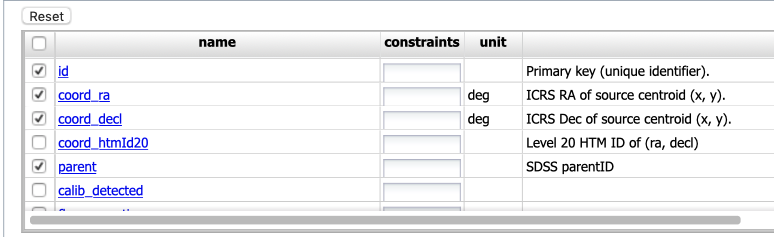
\includegraphics[width=3.12500in]{jira_imgs/244.png}\\

                \vspace{\dp0}
                } \end{minipage} \\ \cdashline{2-3}
                & {\small Test Data} &
                \begin{minipage}[t]{13cm}{\scriptsize
                } \end{minipage} \\ \cdashline{2-3}
                & {\small Expected Result} &
                    \begin{minipage}[t]{13cm}{\scriptsize
                    The column box should be configured to return a minimal useful set of
columns.

                    \vspace{\dp0}
                    } \end{minipage}
                \\ \hdashline


                \multirow{3}{*}{\parbox{1.3cm}{ 2-2
                {\scriptsize from \hyperref[lvv-t851]
                {LVV-T851} } } }

                & {\small Description} &
                \begin{minipage}[t]{13cm}{\scriptsize
                Enter an object name for the portal to resolve. ~We will use NGC 359, a
large elliptical galaxy in the Stripe 82 coverage.\\[2\baselineskip]To
do this, enter the name ``NGC 359'' in the ``Name or Position'' text
input box.\\[2\baselineskip]Leave the other defaults in
place.\\[2\baselineskip]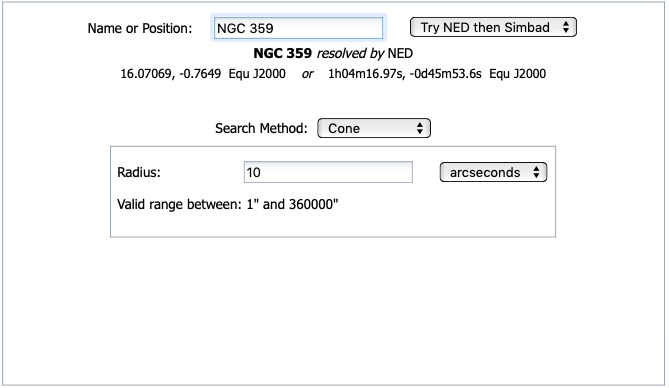
\includegraphics[width=3.12500in]{jira_imgs/245.png}

                \vspace{\dp0}
                } \end{minipage} \\ \cdashline{2-3}
                & {\small Test Data} &
                \begin{minipage}[t]{13cm}{\scriptsize
                } \end{minipage} \\ \cdashline{2-3}
                & {\small Expected Result} &
                    \begin{minipage}[t]{13cm}{\scriptsize
                    There should be a message like ``NGC 359 resolved by NED''. ~The example
coordinates should also changed to the coordinates of NGC 359.

                    \vspace{\dp0}
                    } \end{minipage}
                \\ \hdashline


                \multirow{3}{*}{\parbox{1.3cm}{ 2-3
                {\scriptsize from \hyperref[lvv-t851]
                {LVV-T851} } } }

                & {\small Description} &
                \begin{minipage}[t]{13cm}{\scriptsize
                Submit the query to the portal query engine by clicking the ``Search''
button in the lower left corner of the interface.

                \vspace{\dp0}
                } \end{minipage} \\ \cdashline{2-3}
                & {\small Test Data} &
                \begin{minipage}[t]{13cm}{\scriptsize
                } \end{minipage} \\ \cdashline{2-3}
                & {\small Expected Result} &
                    \begin{minipage}[t]{13cm}{\scriptsize
                    A firefly app with the summary image overlay and catalog widgets side by
side. ~A plot of RA vs. Dec is displayed below the side by side
widgets.\\[2\baselineskip]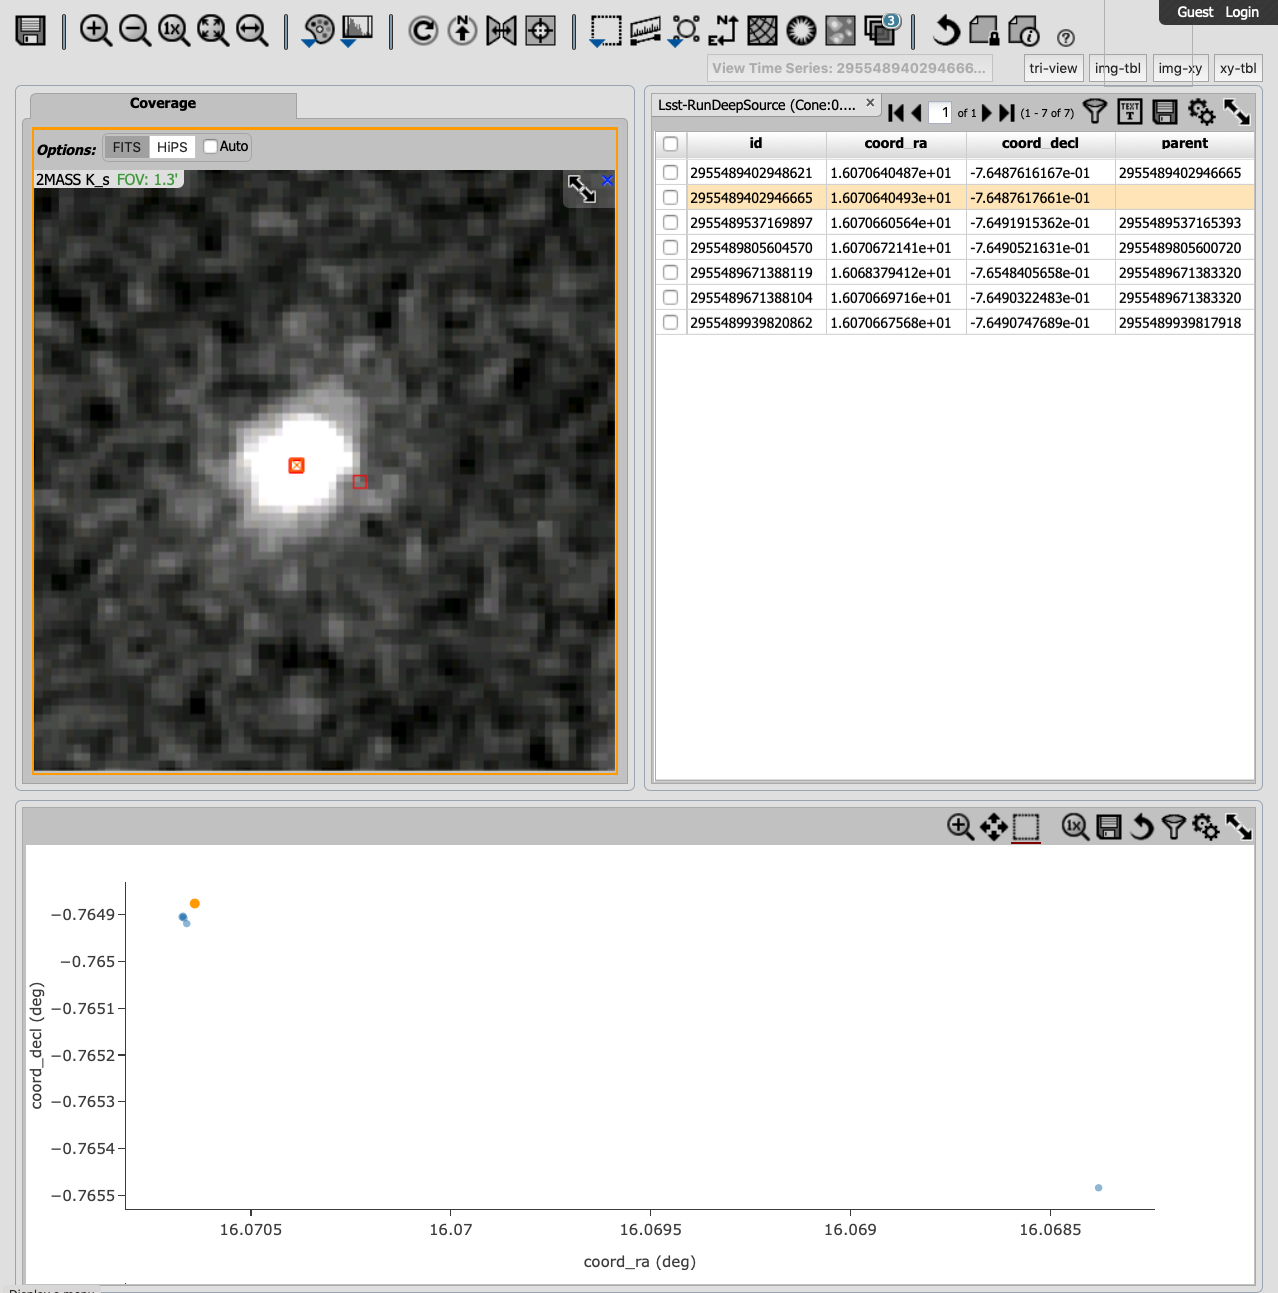
\includegraphics[width=3.12500in]{jira_imgs/246.png}

                    \vspace{\dp0}
                    } \end{minipage}
                \\ \hdashline


        \\ \midrule

            \multirow{3}{*}{ 3 } & Description &
            \begin{minipage}[t]{13cm}{\footnotesize
            Click on the column header that reads ``coord\_ra''. This should re-sort
the table so that objects are sorted in ascending order by RA. Click on
the ``coord\_ra'' header again, and the sorting should change to
descending order by RA.

            \vspace{\dp0}
            } \end{minipage} \\ \cline{2-3}
            & Test Data &
            \begin{minipage}[t]{13cm}{\footnotesize
                No data.
                \vspace{\dp0}
            } \end{minipage} \\ \cline{2-3}
            & Expected Result &
                \begin{minipage}[t]{13cm}{\footnotesize
                Default view (when you first search):\\
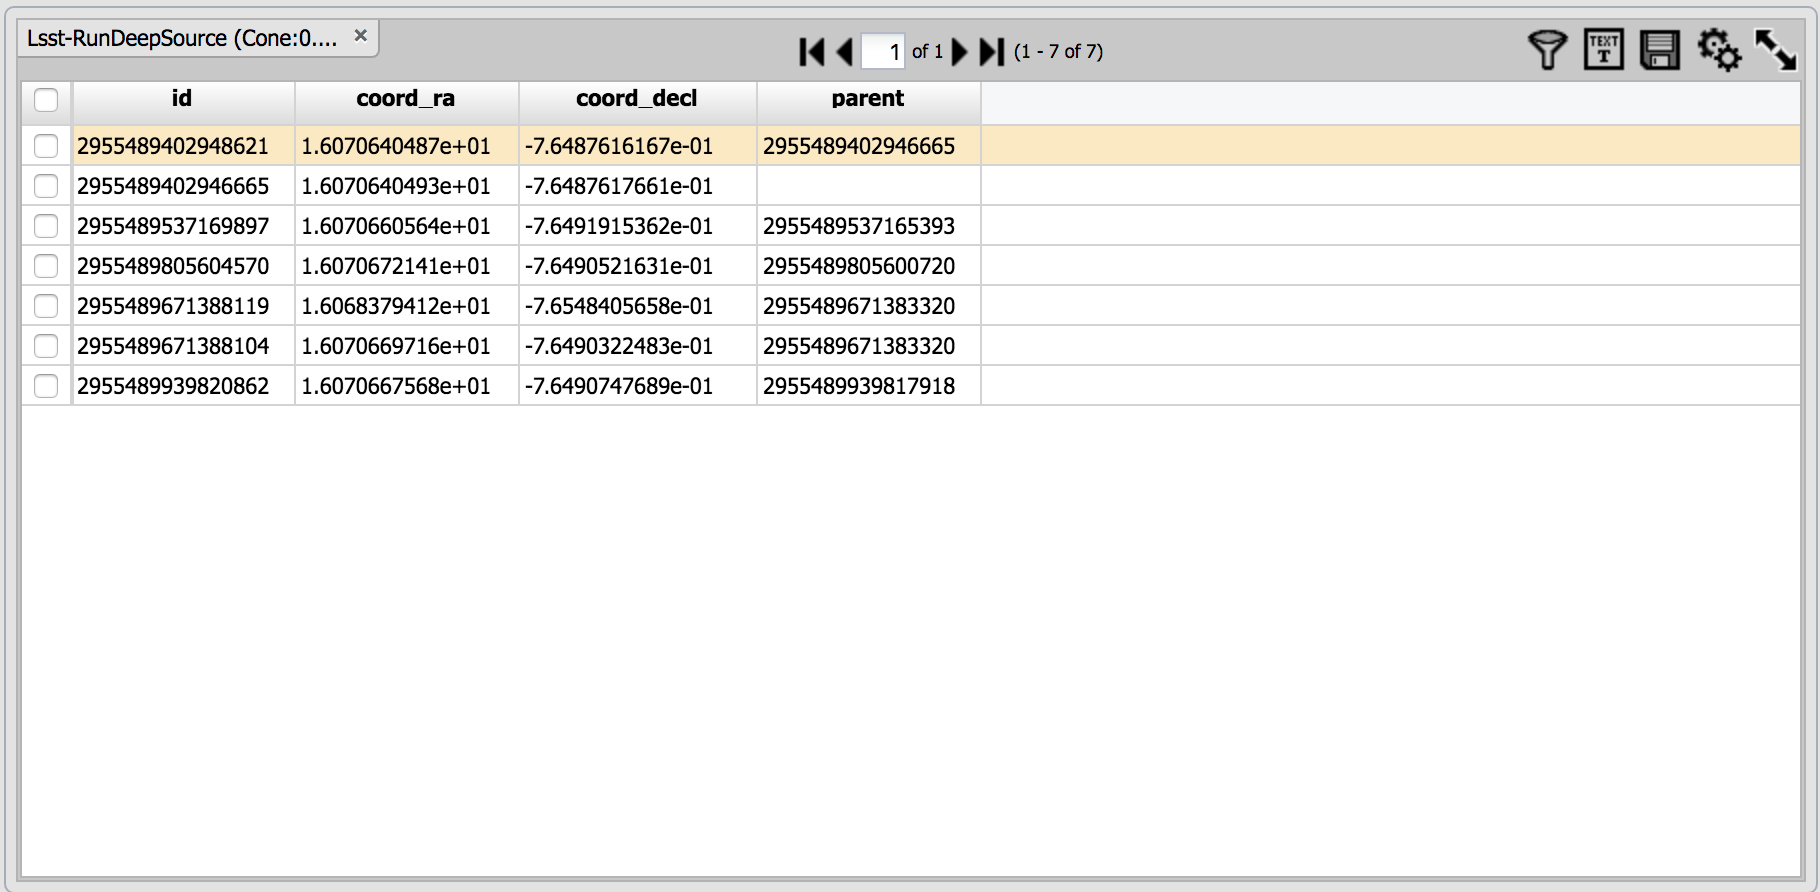
\includegraphics[width=3.90625in]{jira_imgs/256.png}After clicking once
on ``coord\_ra'', it sorts by RA in ascending order:\\
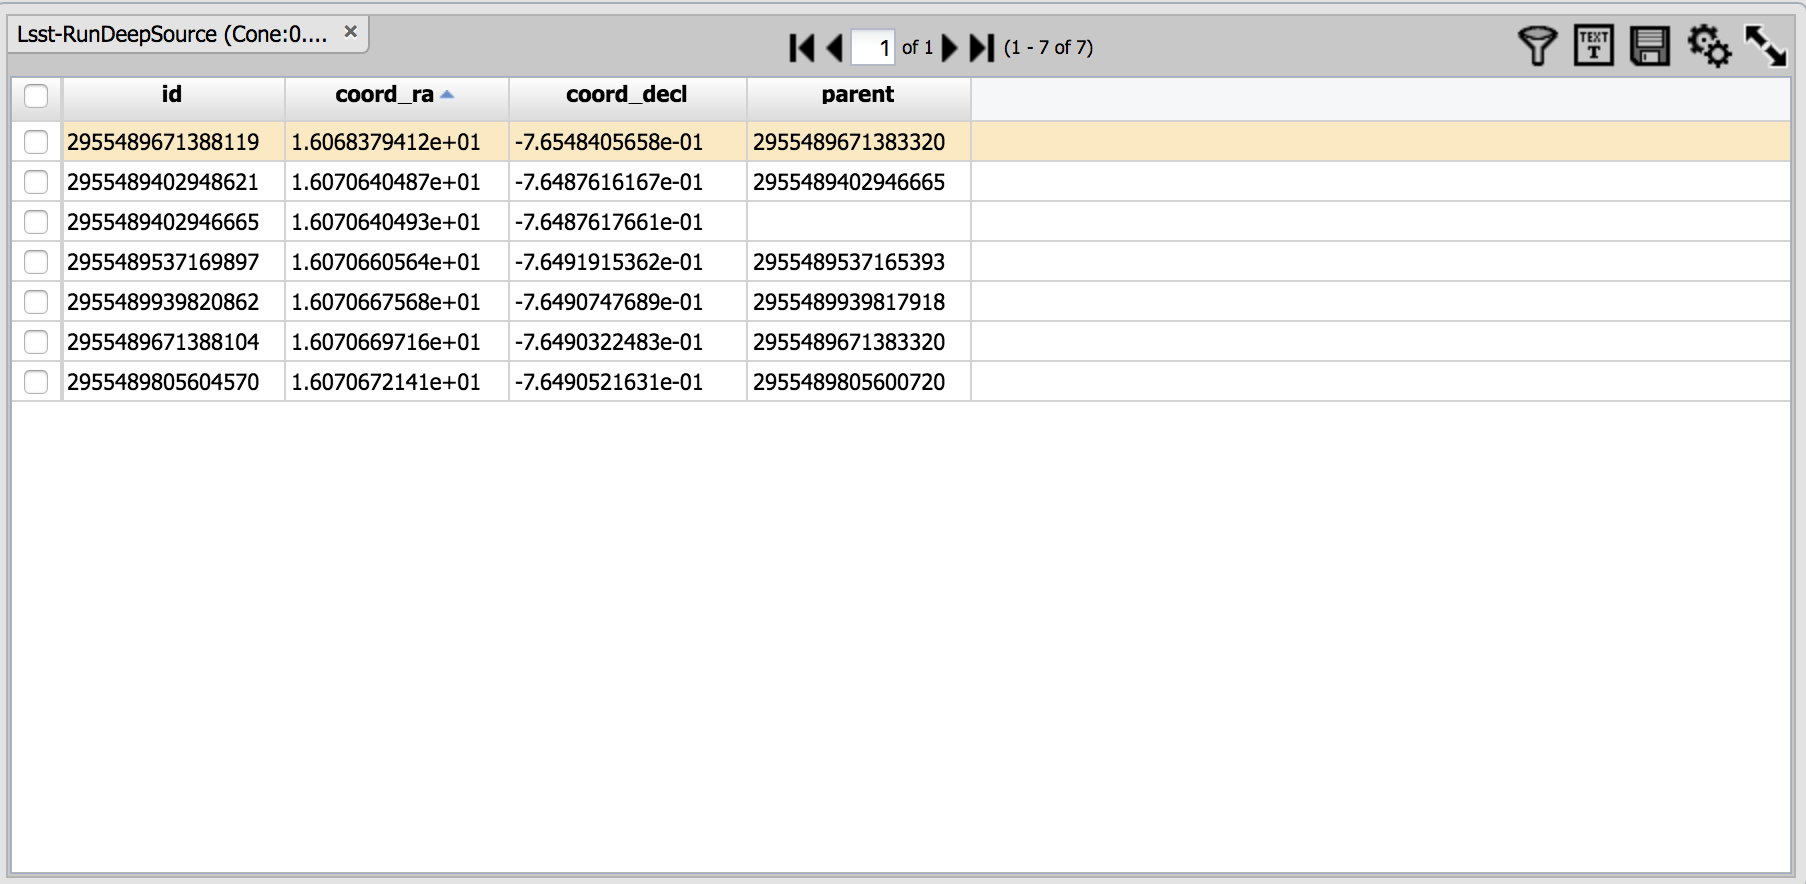
\includegraphics[width=3.89583in]{jira_imgs/257.png}After clicking again
on ``coord\_ra'', it sorts by RA in descending order:\\
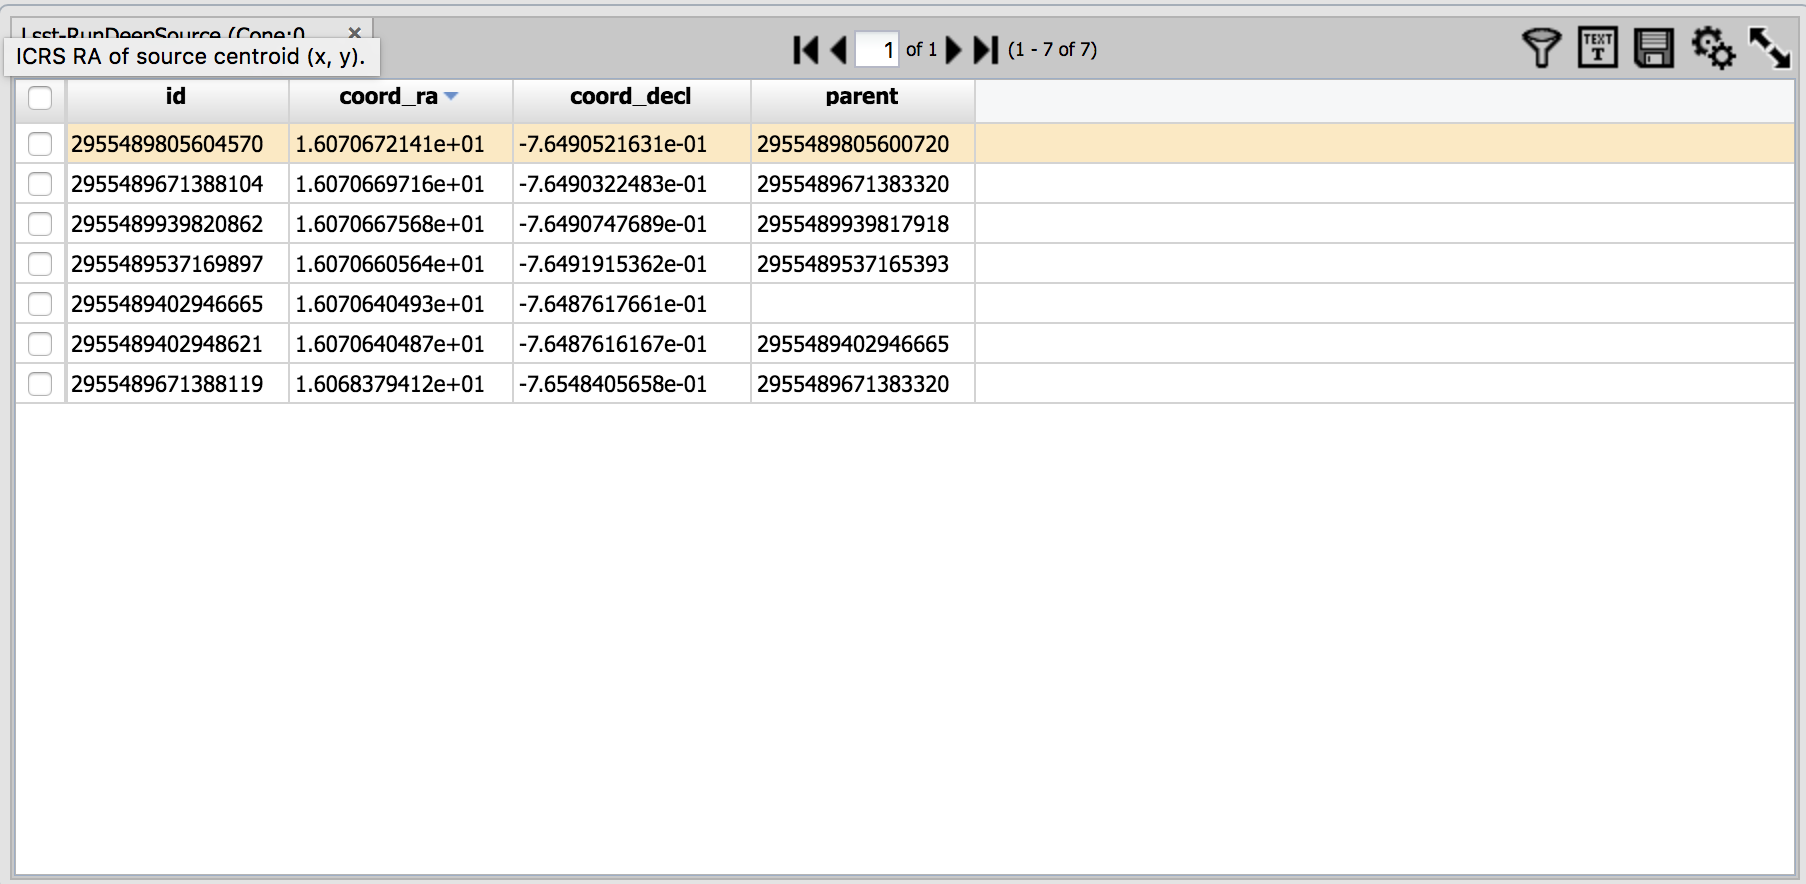
\includegraphics[width=3.86458in]{jira_imgs/258.png}

                \vspace{\dp0}
                } \end{minipage}
        \\ \midrule

            \multirow{3}{*}{ 4 } & Description &
            \begin{minipage}[t]{13cm}{\footnotesize
            Try sorting by another column (e.g., ``Id'') by clicking on that column
header, and confirm that the table updates.

            \vspace{\dp0}
            } \end{minipage} \\ \cline{2-3}
            & Test Data &
            \begin{minipage}[t]{13cm}{\footnotesize
                No data.
                \vspace{\dp0}
            } \end{minipage} \\ \cline{2-3}
            & Expected Result &
                \begin{minipage}[t]{13cm}{\footnotesize
                Table now sorted by the column that was clicked.

                \vspace{\dp0}
                } \end{minipage}
        \\ \midrule

                \multirow{3}{*}{\parbox{1.3cm}{ 5-1
                {\scriptsize from \hyperref[lvv-t850]
                {LVV-T850} } } }

                & {\small Description} &
                \begin{minipage}[t]{13cm}{\scriptsize
                Currently, there is no logout mechanism on the portal.\\
This should be updated as the system matures.\\[2\baselineskip]Simply
close the browser window.

                \vspace{\dp0}
                } \end{minipage} \\ \cdashline{2-3}
                & {\small Test Data} &
                \begin{minipage}[t]{13cm}{\scriptsize
                } \end{minipage} \\ \cdashline{2-3}
                & {\small Expected Result} &
                    \begin{minipage}[t]{13cm}{\scriptsize
                    Closed browser window. ~When navigating to the portal endpoint, expect
to execute the steps in LVV-T849.

                    \vspace{\dp0}
                    } \end{minipage}
                \\ \hdashline


        \\ \midrule
    \end{longtable}

\subsection{LVV-T724 - Verify simple filtering of tabular data}\label{lvv-t724}

\begin{longtable}[]{llllll}
\toprule
Version & Status & Priority & Verification Type & Owner
\\\midrule
1 & Draft & Normal &
Inspection & Jeffrey Carlin
\\\bottomrule
\multicolumn{6}{c}{ Open \href{https://jira.lsstcorp.org/secure/Tests.jspa\#/testCase/LVV-T724}{LVV-T724} in Jira } \\
\end{longtable}

\subsubsection{Verification Elements}
\begin{itemize}
\item \href{https://jira.lsstcorp.org/browse/LVV-9933}{LVV-9933} - DMS-PRTL-REQ-0090-V-01: Simple Filtering of Tabular Data\_1

\end{itemize}

\subsubsection{Test Items}
Verify that the Portal aspect provides the capability to filter tabular
data by a single column, including but not limited to less than
(\textless{}), less than or equal (\textless{}=), greater than
(\textgreater{}), greater than or equal (=\textgreater{}), equal (=),
not equal (!=) and not null (!=null).


\subsubsection{Predecessors}

\subsubsection{Environment Needs}

\paragraph{Software}

\paragraph{Hardware}

\subsubsection{Input Specification}

\subsubsection{Output Specification}

\subsubsection{Test Procedure}
    \begin{longtable}[]{p{1.3cm}p{2cm}p{13cm}}
    %\toprule
    Step & \multicolumn{2}{@{}l}{Description, Input Data and Expected Result} \\ \toprule
    \endhead

                \multirow{3}{*}{\parbox{1.3cm}{ 1-1
                {\scriptsize from \hyperref[lvv-t849]
                {LVV-T849} } } }

                & {\small Description} &
                \begin{minipage}[t]{13cm}{\scriptsize
                Navigate to the Portal Aspect endpoint. ~The stable version should be
used for this test and is currently located at:
https://lsst-lsp-stable.ncsa.illinois.edu/portal/app/ .

                \vspace{\dp0}
                } \end{minipage} \\ \cdashline{2-3}
                & {\small Test Data} &
                \begin{minipage}[t]{13cm}{\scriptsize
                } \end{minipage} \\ \cdashline{2-3}
                & {\small Expected Result} &
                    \begin{minipage}[t]{13cm}{\scriptsize
                    A credential-entry screen should be displayed.

                    \vspace{\dp0}
                    } \end{minipage}
                \\ \hdashline


                \multirow{3}{*}{\parbox{1.3cm}{ 1-2
                {\scriptsize from \hyperref[lvv-t849]
                {LVV-T849} } } }

                & {\small Description} &
                \begin{minipage}[t]{13cm}{\scriptsize
                Enter a valid set of credentials for an LSST user with LSP access on the
instance under test.

                \vspace{\dp0}
                } \end{minipage} \\ \cdashline{2-3}
                & {\small Test Data} &
                \begin{minipage}[t]{13cm}{\scriptsize
                } \end{minipage} \\ \cdashline{2-3}
                & {\small Expected Result} &
                    \begin{minipage}[t]{13cm}{\scriptsize
                    The Portal Aspect UI should be displayed following authentication.

                    \vspace{\dp0}
                    } \end{minipage}
                \\ \hdashline


        \\ \midrule

                \multirow{3}{*}{\parbox{1.3cm}{ 2-1
                {\scriptsize from \hyperref[lvv-t851]
                {LVV-T851} } } }

                & {\small Description} &
                \begin{minipage}[t]{13cm}{\scriptsize
                The default catalog (SDSS Stripe 82, 2013 LSST Processing) is fine for
this.\\[2\baselineskip]Choose columns to return by:\\
1) unchecking the top box in the column selection box\\
2) checking columns for id, coord\_ra, coord\_dec, and
parent.\\[2\baselineskip]The result should look like the following:\\
\hspace*{0.333em}\\
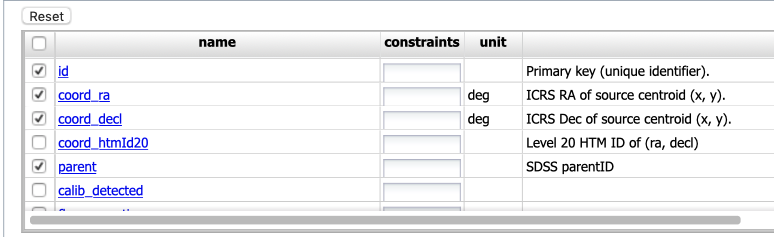
\includegraphics[width=3.12500in]{jira_imgs/244.png}\\

                \vspace{\dp0}
                } \end{minipage} \\ \cdashline{2-3}
                & {\small Test Data} &
                \begin{minipage}[t]{13cm}{\scriptsize
                } \end{minipage} \\ \cdashline{2-3}
                & {\small Expected Result} &
                    \begin{minipage}[t]{13cm}{\scriptsize
                    The column box should be configured to return a minimal useful set of
columns.

                    \vspace{\dp0}
                    } \end{minipage}
                \\ \hdashline


                \multirow{3}{*}{\parbox{1.3cm}{ 2-2
                {\scriptsize from \hyperref[lvv-t851]
                {LVV-T851} } } }

                & {\small Description} &
                \begin{minipage}[t]{13cm}{\scriptsize
                Enter an object name for the portal to resolve. ~We will use NGC 359, a
large elliptical galaxy in the Stripe 82 coverage.\\[2\baselineskip]To
do this, enter the name ``NGC 359'' in the ``Name or Position'' text
input box.\\[2\baselineskip]Leave the other defaults in
place.\\[2\baselineskip]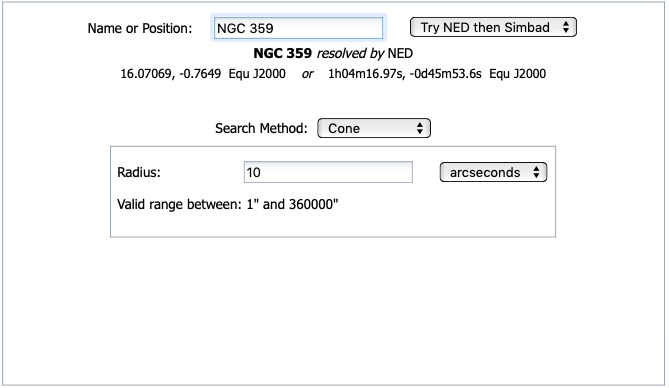
\includegraphics[width=3.12500in]{jira_imgs/245.png}

                \vspace{\dp0}
                } \end{minipage} \\ \cdashline{2-3}
                & {\small Test Data} &
                \begin{minipage}[t]{13cm}{\scriptsize
                } \end{minipage} \\ \cdashline{2-3}
                & {\small Expected Result} &
                    \begin{minipage}[t]{13cm}{\scriptsize
                    There should be a message like ``NGC 359 resolved by NED''. ~The example
coordinates should also changed to the coordinates of NGC 359.

                    \vspace{\dp0}
                    } \end{minipage}
                \\ \hdashline


                \multirow{3}{*}{\parbox{1.3cm}{ 2-3
                {\scriptsize from \hyperref[lvv-t851]
                {LVV-T851} } } }

                & {\small Description} &
                \begin{minipage}[t]{13cm}{\scriptsize
                Submit the query to the portal query engine by clicking the ``Search''
button in the lower left corner of the interface.

                \vspace{\dp0}
                } \end{minipage} \\ \cdashline{2-3}
                & {\small Test Data} &
                \begin{minipage}[t]{13cm}{\scriptsize
                } \end{minipage} \\ \cdashline{2-3}
                & {\small Expected Result} &
                    \begin{minipage}[t]{13cm}{\scriptsize
                    A firefly app with the summary image overlay and catalog widgets side by
side. ~A plot of RA vs. Dec is displayed below the side by side
widgets.\\[2\baselineskip]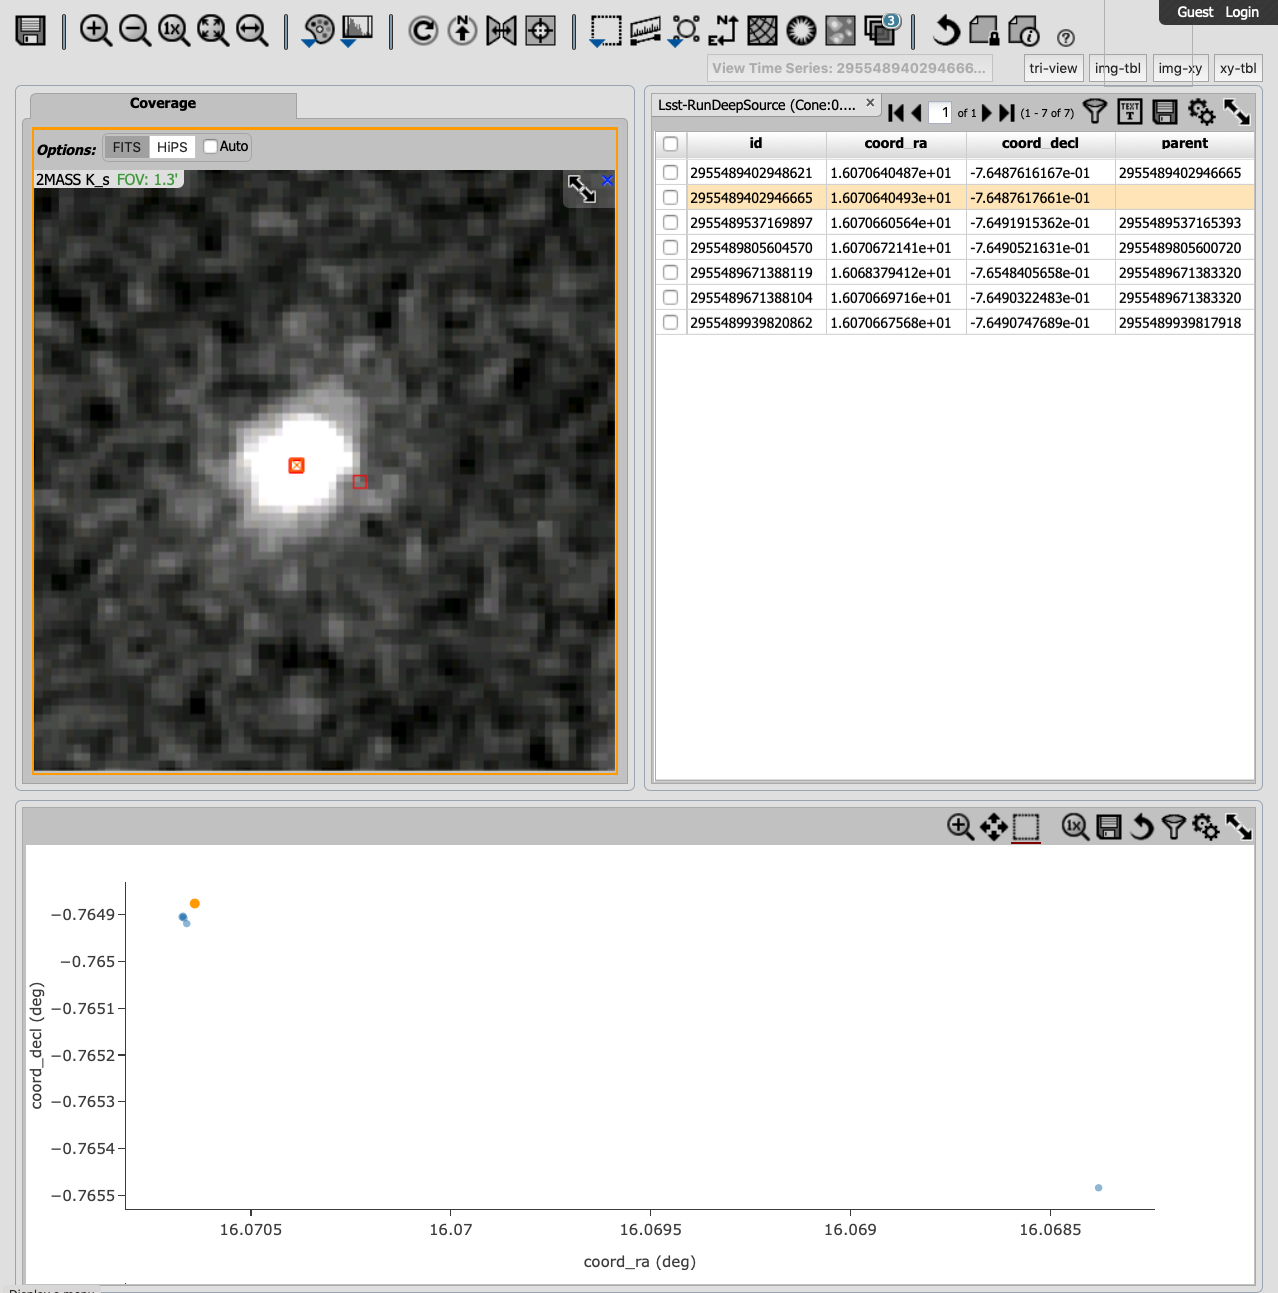
\includegraphics[width=3.12500in]{jira_imgs/246.png}

                    \vspace{\dp0}
                    } \end{minipage}
                \\ \hdashline


        \\ \midrule

            \multirow{3}{*}{ 3 } & Description &
            \begin{minipage}[t]{13cm}{\footnotesize
            Verify the table can be filtered by:\\
1. choosing the ``filter'' icon:~\\

\includegraphics[width=0.28125in]{jira_imgs/254.png}2. entering a filter
criterion in the filter box: e.g. coadd\_ra is less than 16.06905.\\
3. pressing return to execute the filtering

            \vspace{\dp0}
            } \end{minipage} \\ \cline{2-3}
            & Test Data &
            \begin{minipage}[t]{13cm}{\footnotesize
                No data.
                \vspace{\dp0}
            } \end{minipage} \\ \cline{2-3}
            & Expected Result &
                \begin{minipage}[t]{13cm}{\footnotesize
                Expect only a single row to be selected:\\
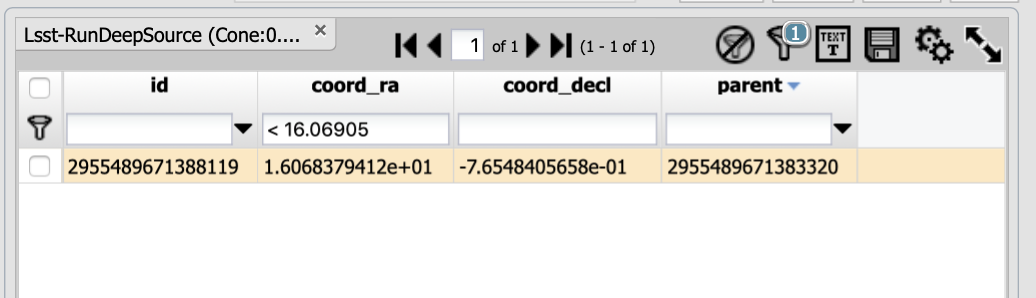
\includegraphics[width=3.12500in]{jira_imgs/255.png}

                \vspace{\dp0}
                } \end{minipage}
        \\ \midrule

                \multirow{3}{*}{\parbox{1.3cm}{ 4-1
                {\scriptsize from \hyperref[lvv-t850]
                {LVV-T850} } } }

                & {\small Description} &
                \begin{minipage}[t]{13cm}{\scriptsize
                Currently, there is no logout mechanism on the portal.\\
This should be updated as the system matures.\\[2\baselineskip]Simply
close the browser window.

                \vspace{\dp0}
                } \end{minipage} \\ \cdashline{2-3}
                & {\small Test Data} &
                \begin{minipage}[t]{13cm}{\scriptsize
                } \end{minipage} \\ \cdashline{2-3}
                & {\small Expected Result} &
                    \begin{minipage}[t]{13cm}{\scriptsize
                    Closed browser window. ~When navigating to the portal endpoint, expect
to execute the steps in LVV-T849.

                    \vspace{\dp0}
                    } \end{minipage}
                \\ \hdashline


        \\ \midrule
    \end{longtable}

\subsection{LVV-T725 - Verify calculated filtering of tabular data}\label{lvv-t725}

\begin{longtable}[]{llllll}
\toprule
Version & Status & Priority & Verification Type & Owner
\\\midrule
1 & Draft & Normal &
Inspection & Jeffrey Carlin
\\\bottomrule
\multicolumn{6}{c}{ Open \href{https://jira.lsstcorp.org/secure/Tests.jspa\#/testCase/LVV-T725}{LVV-T725} in Jira } \\
\end{longtable}

\subsubsection{Verification Elements}
\begin{itemize}
\item \href{https://jira.lsstcorp.org/browse/LVV-9929}{LVV-9929} - DMS-PRTL-REQ-0091-V-01: Calculated Filtering of Tabular Data\_1

\end{itemize}

\subsubsection{Test Items}
Verify that the Portal aspect provides the capability to filter a table
by single column where the filter has simple arithmetic calculations
applied to the column values, including but not limited to sqrt, log,
log10, exponentials and trigonometric functions.


\subsubsection{Predecessors}

\subsubsection{Environment Needs}

\paragraph{Software}

\paragraph{Hardware}

\subsubsection{Input Specification}

\subsubsection{Output Specification}

\subsubsection{Test Procedure}
    \begin{longtable}[]{p{1.3cm}p{2cm}p{13cm}}
    %\toprule
    Step & \multicolumn{2}{@{}l}{Description, Input Data and Expected Result} \\ \toprule
    \endhead

            \multirow{3}{*}{ 1 } & Description &
            \begin{minipage}[t]{13cm}{\footnotesize
            
            \vspace{\dp0}
            } \end{minipage} \\ \cline{2-3}
            & Test Data &
            \begin{minipage}[t]{13cm}{\footnotesize
                No data.
                \vspace{\dp0}
            } \end{minipage} \\ \cline{2-3}
            & Expected Result &
        \\ \midrule
    \end{longtable}

\subsection{LVV-T726 - Verify filtering data by multiple table columns}\label{lvv-t726}

\begin{longtable}[]{llllll}
\toprule
Version & Status & Priority & Verification Type & Owner
\\\midrule
1 & Draft & Normal &
Inspection & Jeffrey Carlin
\\\bottomrule
\multicolumn{6}{c}{ Open \href{https://jira.lsstcorp.org/secure/Tests.jspa\#/testCase/LVV-T726}{LVV-T726} in Jira } \\
\end{longtable}

\subsubsection{Verification Elements}
\begin{itemize}
\item \href{https://jira.lsstcorp.org/browse/LVV-9931}{LVV-9931} - DMS-PRTL-REQ-0092-V-01: Filtering of Tabular Data by Multiple Columns\_1

\end{itemize}

\subsubsection{Test Items}
Verify that the Portal aspect provides the capability to filter tabular
data by multiple columns within the table and redisplay the filtered
table.


\subsubsection{Predecessors}

\subsubsection{Environment Needs}

\paragraph{Software}

\paragraph{Hardware}

\subsubsection{Input Specification}

\subsubsection{Output Specification}

\subsubsection{Test Procedure}
    \begin{longtable}[]{p{1.3cm}p{2cm}p{13cm}}
    %\toprule
    Step & \multicolumn{2}{@{}l}{Description, Input Data and Expected Result} \\ \toprule
    \endhead

            \multirow{3}{*}{ 1 } & Description &
            \begin{minipage}[t]{13cm}{\footnotesize
            
            \vspace{\dp0}
            } \end{minipage} \\ \cline{2-3}
            & Test Data &
            \begin{minipage}[t]{13cm}{\footnotesize
                No data.
                \vspace{\dp0}
            } \end{minipage} \\ \cline{2-3}
            & Expected Result &
        \\ \midrule
    \end{longtable}

\subsection{LVV-T727 - Verify calculated tabular data columns}\label{lvv-t727}

\begin{longtable}[]{llllll}
\toprule
Version & Status & Priority & Verification Type & Owner
\\\midrule
1 & Draft & Normal &
Inspection & Jeffrey Carlin
\\\bottomrule
\multicolumn{6}{c}{ Open \href{https://jira.lsstcorp.org/secure/Tests.jspa\#/testCase/LVV-T727}{LVV-T727} in Jira } \\
\end{longtable}

\subsubsection{Verification Elements}
\begin{itemize}
\item \href{https://jira.lsstcorp.org/browse/LVV-9930}{LVV-9930} - DMS-PRTL-REQ-0093-V-01: Calculated Quantities on Tabular Data\_1

\end{itemize}

\subsubsection{Test Items}
Verify that the Portal enables the arithmetic calculation and display of
new tabular data columns based on existing columns in a table.~


\subsubsection{Predecessors}

\subsubsection{Environment Needs}

\paragraph{Software}

\paragraph{Hardware}

\subsubsection{Input Specification}

\subsubsection{Output Specification}

\subsubsection{Test Procedure}
    \begin{longtable}[]{p{1.3cm}p{2cm}p{13cm}}
    %\toprule
    Step & \multicolumn{2}{@{}l}{Description, Input Data and Expected Result} \\ \toprule
    \endhead

            \multirow{3}{*}{ 1 } & Description &
            \begin{minipage}[t]{13cm}{\footnotesize
            
            \vspace{\dp0}
            } \end{minipage} \\ \cline{2-3}
            & Test Data &
            \begin{minipage}[t]{13cm}{\footnotesize
                No data.
                \vspace{\dp0}
            } \end{minipage} \\ \cline{2-3}
            & Expected Result &
        \\ \midrule
    \end{longtable}

\subsection{LVV-T728 - Verify statistical measurements on tabular data}\label{lvv-t728}

\begin{longtable}[]{llllll}
\toprule
Version & Status & Priority & Verification Type & Owner
\\\midrule
1 & Draft & Normal &
Inspection & Jeffrey Carlin
\\\bottomrule
\multicolumn{6}{c}{ Open \href{https://jira.lsstcorp.org/secure/Tests.jspa\#/testCase/LVV-T728}{LVV-T728} in Jira } \\
\end{longtable}

\subsubsection{Verification Elements}
\begin{itemize}
\item \href{https://jira.lsstcorp.org/browse/LVV-9935}{LVV-9935} - DMS-PRTL-REQ-0094-V-01: Statistical Measurements on Tabular Data\_1

\end{itemize}

\subsubsection{Test Items}
Verify that the Portal aspect enables the capability to perform a set of
statistical measurements (e.g., mean, median, RMS, skew, kurtosis) on
tabular data selected by the user.


\subsubsection{Predecessors}

\subsubsection{Environment Needs}

\paragraph{Software}

\paragraph{Hardware}

\subsubsection{Input Specification}

\subsubsection{Output Specification}

\subsubsection{Test Procedure}
    \begin{longtable}[]{p{1.3cm}p{2cm}p{13cm}}
    %\toprule
    Step & \multicolumn{2}{@{}l}{Description, Input Data and Expected Result} \\ \toprule
    \endhead

            \multirow{3}{*}{ 1 } & Description &
            \begin{minipage}[t]{13cm}{\footnotesize
            
            \vspace{\dp0}
            } \end{minipage} \\ \cline{2-3}
            & Test Data &
            \begin{minipage}[t]{13cm}{\footnotesize
                No data.
                \vspace{\dp0}
            } \end{minipage} \\ \cline{2-3}
            & Expected Result &
        \\ \midrule
    \end{longtable}

\subsection{LVV-T729 - Verify saving of displayed tabular data}\label{lvv-t729}

\begin{longtable}[]{llllll}
\toprule
Version & Status & Priority & Verification Type & Owner
\\\midrule
1 & Draft & Normal &
Inspection & Jeffrey Carlin
\\\bottomrule
\multicolumn{6}{c}{ Open \href{https://jira.lsstcorp.org/secure/Tests.jspa\#/testCase/LVV-T729}{LVV-T729} in Jira } \\
\end{longtable}

\subsubsection{Verification Elements}
\begin{itemize}
\item \href{https://jira.lsstcorp.org/browse/LVV-9932}{LVV-9932} - DMS-PRTL-REQ-0095-V-01: Saving Displayed Tabular Data\_1

\end{itemize}

\subsubsection{Test Items}
Verify that the Portal aspect provides the capability to save and or
download tabular data as it is displayed in the interface maintaining
the content, filtering, and sorting.


\subsubsection{Predecessors}

\subsubsection{Environment Needs}

\paragraph{Software}

\paragraph{Hardware}

\subsubsection{Input Specification}

\subsubsection{Output Specification}

\subsubsection{Test Procedure}
    \begin{longtable}[]{p{1.3cm}p{2cm}p{13cm}}
    %\toprule
    Step & \multicolumn{2}{@{}l}{Description, Input Data and Expected Result} \\ \toprule
    \endhead

            \multirow{3}{*}{ 1 } & Description &
            \begin{minipage}[t]{13cm}{\footnotesize
            
            \vspace{\dp0}
            } \end{minipage} \\ \cline{2-3}
            & Test Data &
            \begin{minipage}[t]{13cm}{\footnotesize
                No data.
                \vspace{\dp0}
            } \end{minipage} \\ \cline{2-3}
            & Expected Result &
        \\ \midrule
    \end{longtable}

\subsection{LVV-T730 - Verify creation and display of false-color images}\label{lvv-t730}

\begin{longtable}[]{llllll}
\toprule
Version & Status & Priority & Verification Type & Owner
\\\midrule
1 & Draft & Normal &
Inspection & Jeffrey Carlin
\\\bottomrule
\multicolumn{6}{c}{ Open \href{https://jira.lsstcorp.org/secure/Tests.jspa\#/testCase/LVV-T730}{LVV-T730} in Jira } \\
\end{longtable}

\subsubsection{Verification Elements}
\begin{itemize}
\item \href{https://jira.lsstcorp.org/browse/LVV-9936}{LVV-9936} - DMS-PRTL-REQ-0096-V-01: False-color Images Creation and Display\_1

\end{itemize}

\subsubsection{Test Items}
Verify that the Portal aspect has the capability to create and display
false-color images composed from any user-selectable set of filters from
multiple filter views of the same region.


\subsubsection{Predecessors}

\subsubsection{Environment Needs}

\paragraph{Software}

\paragraph{Hardware}

\subsubsection{Input Specification}

\subsubsection{Output Specification}

\subsubsection{Test Procedure}
    \begin{longtable}[]{p{1.3cm}p{2cm}p{13cm}}
    %\toprule
    Step & \multicolumn{2}{@{}l}{Description, Input Data and Expected Result} \\ \toprule
    \endhead

            \multirow{3}{*}{ 1 } & Description &
            \begin{minipage}[t]{13cm}{\footnotesize
            
            \vspace{\dp0}
            } \end{minipage} \\ \cline{2-3}
            & Test Data &
            \begin{minipage}[t]{13cm}{\footnotesize
                No data.
                \vspace{\dp0}
            } \end{minipage} \\ \cline{2-3}
            & Expected Result &
        \\ \midrule
    \end{longtable}

\subsection{LVV-T731 - Verify statistical measurements on user-selected regions of images}\label{lvv-t731}

\begin{longtable}[]{llllll}
\toprule
Version & Status & Priority & Verification Type & Owner
\\\midrule
1 & Draft & Normal &
Inspection & Jeffrey Carlin
\\\bottomrule
\multicolumn{6}{c}{ Open \href{https://jira.lsstcorp.org/secure/Tests.jspa\#/testCase/LVV-T731}{LVV-T731} in Jira } \\
\end{longtable}

\subsubsection{Verification Elements}
\begin{itemize}
\item \href{https://jira.lsstcorp.org/browse/LVV-9937}{LVV-9937} - DMS-PRTL-REQ-0097-V-01: Statistical Measurements on Image Data\_1

\end{itemize}

\subsubsection{Test Items}
Verify that the Portal aspect enables the capability to perform a set of
statistical measurements (e.g., mean, median, RMS, skew, kurtosis) on
user-selected regions in images.


\subsubsection{Predecessors}

\subsubsection{Environment Needs}

\paragraph{Software}

\paragraph{Hardware}

\subsubsection{Input Specification}

\subsubsection{Output Specification}

\subsubsection{Test Procedure}
    \begin{longtable}[]{p{1.3cm}p{2cm}p{13cm}}
    %\toprule
    Step & \multicolumn{2}{@{}l}{Description, Input Data and Expected Result} \\ \toprule
    \endhead

            \multirow{3}{*}{ 1 } & Description &
            \begin{minipage}[t]{13cm}{\footnotesize
            
            \vspace{\dp0}
            } \end{minipage} \\ \cline{2-3}
            & Test Data &
            \begin{minipage}[t]{13cm}{\footnotesize
                No data.
                \vspace{\dp0}
            } \end{minipage} \\ \cline{2-3}
            & Expected Result &
        \\ \midrule
    \end{longtable}

\subsection{LVV-T732 - Verify overlay of catalog sources/objects on images}\label{lvv-t732}

\begin{longtable}[]{llllll}
\toprule
Version & Status & Priority & Verification Type & Owner
\\\midrule
1 & Draft & Normal &
Inspection & Jeffrey Carlin
\\\bottomrule
\multicolumn{6}{c}{ Open \href{https://jira.lsstcorp.org/secure/Tests.jspa\#/testCase/LVV-T732}{LVV-T732} in Jira } \\
\end{longtable}

\subsubsection{Verification Elements}
\begin{itemize}
\item \href{https://jira.lsstcorp.org/browse/LVV-9942}{LVV-9942} - DMS-PRTL-REQ-0098-V-01: Overlay Catalog of Sources and Objects on
Images\_1

\end{itemize}

\subsubsection{Test Items}
Verify that the Portal aspect enables the overlay of positions of
catalog sources and objects on a displayed image based upon
astrophysically-based or observatory-based coordinates.


\subsubsection{Predecessors}

\subsubsection{Environment Needs}

\paragraph{Software}

\paragraph{Hardware}

\subsubsection{Input Specification}

\subsubsection{Output Specification}

\subsubsection{Test Procedure}
    \begin{longtable}[]{p{1.3cm}p{2cm}p{13cm}}
    %\toprule
    Step & \multicolumn{2}{@{}l}{Description, Input Data and Expected Result} \\ \toprule
    \endhead

            \multirow{3}{*}{ 1 } & Description &
            \begin{minipage}[t]{13cm}{\footnotesize
            
            \vspace{\dp0}
            } \end{minipage} \\ \cline{2-3}
            & Test Data &
            \begin{minipage}[t]{13cm}{\footnotesize
                No data.
                \vspace{\dp0}
            } \end{minipage} \\ \cline{2-3}
            & Expected Result &
        \\ \midrule
    \end{longtable}

\subsection{LVV-T733 - Verify overlay of LSST-derived orbits on images}\label{lvv-t733}

\begin{longtable}[]{llllll}
\toprule
Version & Status & Priority & Verification Type & Owner
\\\midrule
1 & Draft & Normal &
Inspection & Jeffrey Carlin
\\\bottomrule
\multicolumn{6}{c}{ Open \href{https://jira.lsstcorp.org/secure/Tests.jspa\#/testCase/LVV-T733}{LVV-T733} in Jira } \\
\end{longtable}

\subsubsection{Verification Elements}
\begin{itemize}
\item \href{https://jira.lsstcorp.org/browse/LVV-9943}{LVV-9943} - DMS-PRTL-REQ-0099-V-01: Overlay LSST-Derived Orbits\_1

\end{itemize}

\subsubsection{Test Items}
Verify that the Portal aspect has the capability to overlay predicted
positions from the orbits of solar system objects in the LSST catalog on
to images.


\subsubsection{Predecessors}

\subsubsection{Environment Needs}

\paragraph{Software}

\paragraph{Hardware}

\subsubsection{Input Specification}

\subsubsection{Output Specification}

\subsubsection{Test Procedure}
    \begin{longtable}[]{p{1.3cm}p{2cm}p{13cm}}
    %\toprule
    Step & \multicolumn{2}{@{}l}{Description, Input Data and Expected Result} \\ \toprule
    \endhead

            \multirow{3}{*}{ 1 } & Description &
            \begin{minipage}[t]{13cm}{\footnotesize
            
            \vspace{\dp0}
            } \end{minipage} \\ \cline{2-3}
            & Test Data &
            \begin{minipage}[t]{13cm}{\footnotesize
                No data.
                \vspace{\dp0}
            } \end{minipage} \\ \cline{2-3}
            & Expected Result &
        \\ \midrule
    \end{longtable}

\subsection{LVV-T734 - Verify overlay of user-supplied catalogs on images}\label{lvv-t734}

\begin{longtable}[]{llllll}
\toprule
Version & Status & Priority & Verification Type & Owner
\\\midrule
1 & Draft & Normal &
Inspection & Jeffrey Carlin
\\\bottomrule
\multicolumn{6}{c}{ Open \href{https://jira.lsstcorp.org/secure/Tests.jspa\#/testCase/LVV-T734}{LVV-T734} in Jira } \\
\end{longtable}

\subsubsection{Verification Elements}
\begin{itemize}
\item \href{https://jira.lsstcorp.org/browse/LVV-9944}{LVV-9944} - DMS-PRTL-REQ-0100-V-01: Overlay User-provided Catalogs on Images\_1

\end{itemize}

\subsubsection{Test Items}
Verify that the Portal enables users to overlay the positions of objects
in user-supplied catalogs on top of images.


\subsubsection{Predecessors}

\subsubsection{Environment Needs}

\paragraph{Software}

\paragraph{Hardware}

\subsubsection{Input Specification}

\subsubsection{Output Specification}

\subsubsection{Test Procedure}
    \begin{longtable}[]{p{1.3cm}p{2cm}p{13cm}}
    %\toprule
    Step & \multicolumn{2}{@{}l}{Description, Input Data and Expected Result} \\ \toprule
    \endhead

            \multirow{3}{*}{ 1 } & Description &
            \begin{minipage}[t]{13cm}{\footnotesize
            
            \vspace{\dp0}
            } \end{minipage} \\ \cline{2-3}
            & Test Data &
            \begin{minipage}[t]{13cm}{\footnotesize
                No data.
                \vspace{\dp0}
            } \end{minipage} \\ \cline{2-3}
            & Expected Result &
        \\ \midrule
    \end{longtable}

\subsection{LVV-T735 - Verify overlay of user-supplied region files on images}\label{lvv-t735}

\begin{longtable}[]{llllll}
\toprule
Version & Status & Priority & Verification Type & Owner
\\\midrule
1 & Draft & Normal &
Inspection & Jeffrey Carlin
\\\bottomrule
\multicolumn{6}{c}{ Open \href{https://jira.lsstcorp.org/secure/Tests.jspa\#/testCase/LVV-T735}{LVV-T735} in Jira } \\
\end{longtable}

\subsubsection{Verification Elements}
\begin{itemize}
\item \href{https://jira.lsstcorp.org/browse/LVV-9945}{LVV-9945} - DMS-PRTL-REQ-0101-V-01: Overlay User-provided Region Files on Images\_1

\end{itemize}

\subsubsection{Test Items}
Verify that Portal users can upload a region file and overlay the region
on a displayed image.


\subsubsection{Predecessors}

\subsubsection{Environment Needs}

\paragraph{Software}

\paragraph{Hardware}

\subsubsection{Input Specification}

\subsubsection{Output Specification}

\subsubsection{Test Procedure}
    \begin{longtable}[]{p{1.3cm}p{2cm}p{13cm}}
    %\toprule
    Step & \multicolumn{2}{@{}l}{Description, Input Data and Expected Result} \\ \toprule
    \endhead

            \multirow{3}{*}{ 1 } & Description &
            \begin{minipage}[t]{13cm}{\footnotesize
            
            \vspace{\dp0}
            } \end{minipage} \\ \cline{2-3}
            & Test Data &
            \begin{minipage}[t]{13cm}{\footnotesize
                No data.
                \vspace{\dp0}
            } \end{minipage} \\ \cline{2-3}
            & Expected Result &
        \\ \midrule
    \end{longtable}

\subsection{LVV-T736 - Verify overlay of camera artifacts on images}\label{lvv-t736}

\begin{longtable}[]{llllll}
\toprule
Version & Status & Priority & Verification Type & Owner
\\\midrule
1 & Draft & Normal &
Inspection & Jeffrey Carlin
\\\bottomrule
\multicolumn{6}{c}{ Open \href{https://jira.lsstcorp.org/secure/Tests.jspa\#/testCase/LVV-T736}{LVV-T736} in Jira } \\
\end{longtable}

\subsubsection{Verification Elements}
\begin{itemize}
\item \href{https://jira.lsstcorp.org/browse/LVV-9940}{LVV-9940} - DMS-PRTL-REQ-0102-V-01: Display of Camera Artifacts as Overlays\_1

\end{itemize}

\subsubsection{Test Items}
Verify that the Portal aspect has the capability to display as image
overlays camera artifacts including but not limited to image crosstalk
matrices, ghost image identifications, saturation, and column bleeding.


\subsubsection{Predecessors}

\subsubsection{Environment Needs}

\paragraph{Software}

\paragraph{Hardware}

\subsubsection{Input Specification}

\subsubsection{Output Specification}

\subsubsection{Test Procedure}
    \begin{longtable}[]{p{1.3cm}p{2cm}p{13cm}}
    %\toprule
    Step & \multicolumn{2}{@{}l}{Description, Input Data and Expected Result} \\ \toprule
    \endhead

            \multirow{3}{*}{ 1 } & Description &
            \begin{minipage}[t]{13cm}{\footnotesize
            
            \vspace{\dp0}
            } \end{minipage} \\ \cline{2-3}
            & Test Data &
            \begin{minipage}[t]{13cm}{\footnotesize
                No data.
                \vspace{\dp0}
            } \end{minipage} \\ \cline{2-3}
            & Expected Result &
        \\ \midrule
    \end{longtable}

\subsection{LVV-T737 - Verify single-object time-domain image view}\label{lvv-t737}

\begin{longtable}[]{llllll}
\toprule
Version & Status & Priority & Verification Type & Owner
\\\midrule
1 & Draft & Normal &
Inspection & Jeffrey Carlin
\\\bottomrule
\multicolumn{6}{c}{ Open \href{https://jira.lsstcorp.org/secure/Tests.jspa\#/testCase/LVV-T737}{LVV-T737} in Jira } \\
\end{longtable}

\subsubsection{Verification Elements}
\begin{itemize}
\item \href{https://jira.lsstcorp.org/browse/LVV-9948}{LVV-9948} - DMS-PRTL-REQ-0103-V-01: Single-Object Time-Domain Image View\_1

\end{itemize}

\subsubsection{Test Items}
Verify that the Portal provides the capability to view an image time
series that maintains the same physical scale, photometric scale, and
image size display of a cutout area centered on an LSST object. If the
object moves, then the images should stay centered on the object.


\subsubsection{Predecessors}

\subsubsection{Environment Needs}

\paragraph{Software}

\paragraph{Hardware}

\subsubsection{Input Specification}

\subsubsection{Output Specification}

\subsubsection{Test Procedure}
    \begin{longtable}[]{p{1.3cm}p{2cm}p{13cm}}
    %\toprule
    Step & \multicolumn{2}{@{}l}{Description, Input Data and Expected Result} \\ \toprule
    \endhead

            \multirow{3}{*}{ 1 } & Description &
            \begin{minipage}[t]{13cm}{\footnotesize
            
            \vspace{\dp0}
            } \end{minipage} \\ \cline{2-3}
            & Test Data &
            \begin{minipage}[t]{13cm}{\footnotesize
                No data.
                \vspace{\dp0}
            } \end{minipage} \\ \cline{2-3}
            & Expected Result &
        \\ \midrule
    \end{longtable}

\subsection{LVV-T738 - Verify position-based time-domain image view}\label{lvv-t738}

\begin{longtable}[]{llllll}
\toprule
Version & Status & Priority & Verification Type & Owner
\\\midrule
1 & Draft & Normal &
Inspection & Jeffrey Carlin
\\\bottomrule
\multicolumn{6}{c}{ Open \href{https://jira.lsstcorp.org/secure/Tests.jspa\#/testCase/LVV-T738}{LVV-T738} in Jira } \\
\end{longtable}

\subsubsection{Verification Elements}
\begin{itemize}
\item \href{https://jira.lsstcorp.org/browse/LVV-9946}{LVV-9946} - DMS-PRTL-REQ-0104-V-01: Position-based Time-Domain Image View\_1

\end{itemize}

\subsubsection{Test Items}
Verify that the Portal provides the capability to view an image time
series that maintains the same physical scale, photometric scale, and
image size display of a specified region on the sky. If the object
moves, then the images should stay centered on the sky and the object
will appear to move.


\subsubsection{Predecessors}

\subsubsection{Environment Needs}

\paragraph{Software}

\paragraph{Hardware}

\subsubsection{Input Specification}

\subsubsection{Output Specification}

\subsubsection{Test Procedure}
    \begin{longtable}[]{p{1.3cm}p{2cm}p{13cm}}
    %\toprule
    Step & \multicolumn{2}{@{}l}{Description, Input Data and Expected Result} \\ \toprule
    \endhead

            \multirow{3}{*}{ 1 } & Description &
            \begin{minipage}[t]{13cm}{\footnotesize
            
            \vspace{\dp0}
            } \end{minipage} \\ \cline{2-3}
            & Test Data &
            \begin{minipage}[t]{13cm}{\footnotesize
                No data.
                \vspace{\dp0}
            } \end{minipage} \\ \cline{2-3}
            & Expected Result &
        \\ \midrule
    \end{longtable}

\subsection{LVV-T739 - Verify display of light curves}\label{lvv-t739}

\begin{longtable}[]{llllll}
\toprule
Version & Status & Priority & Verification Type & Owner
\\\midrule
1 & Draft & Normal &
Inspection & Jeffrey Carlin
\\\bottomrule
\multicolumn{6}{c}{ Open \href{https://jira.lsstcorp.org/secure/Tests.jspa\#/testCase/LVV-T739}{LVV-T739} in Jira } \\
\end{longtable}

\subsubsection{Verification Elements}
\begin{itemize}
\item \href{https://jira.lsstcorp.org/browse/LVV-9938}{LVV-9938} - DMS-PRTL-REQ-0105-V-01: Brightness Light Curves\_1

\end{itemize}

\subsubsection{Test Items}
Verify that the Portal can display graphically the
brightness/flux/magnitude of an LSST Object, Source, or ForcedSource as
a function of time.


\subsubsection{Predecessors}

\subsubsection{Environment Needs}

\paragraph{Software}

\paragraph{Hardware}

\subsubsection{Input Specification}

\subsubsection{Output Specification}

\subsubsection{Test Procedure}
    \begin{longtable}[]{p{1.3cm}p{2cm}p{13cm}}
    %\toprule
    Step & \multicolumn{2}{@{}l}{Description, Input Data and Expected Result} \\ \toprule
    \endhead

            \multirow{3}{*}{ 1 } & Description &
            \begin{minipage}[t]{13cm}{\footnotesize
            
            \vspace{\dp0}
            } \end{minipage} \\ \cline{2-3}
            & Test Data &
            \begin{minipage}[t]{13cm}{\footnotesize
                No data.
                \vspace{\dp0}
            } \end{minipage} \\ \cline{2-3}
            & Expected Result &
        \\ \midrule
    \end{longtable}

\subsection{LVV-T740 - Verify linked tables, plots, and images}\label{lvv-t740}

\begin{longtable}[]{llllll}
\toprule
Version & Status & Priority & Verification Type & Owner
\\\midrule
1 & Draft & Normal &
Inspection & Jeffrey Carlin
\\\bottomrule
\multicolumn{6}{c}{ Open \href{https://jira.lsstcorp.org/secure/Tests.jspa\#/testCase/LVV-T740}{LVV-T740} in Jira } \\
\end{longtable}

\subsubsection{Verification Elements}
\begin{itemize}
\item \href{https://jira.lsstcorp.org/browse/LVV-9941}{LVV-9941} - DMS-PRTL-REQ-0106-V-01: Linked Tables, Plots, and Images\_1

\end{itemize}

\subsubsection{Test Items}
Verify that the Portal aspect has the capability to have tabular data,
plots, and images with overlays connected via brushing and linking, so
that updates to the data in any one visualization tool (e.g., plot,
image, table) creates an update in other visualization tools.


\subsubsection{Predecessors}

\subsubsection{Environment Needs}

\paragraph{Software}

\paragraph{Hardware}

\subsubsection{Input Specification}

\subsubsection{Output Specification}

\subsubsection{Test Procedure}
    \begin{longtable}[]{p{1.3cm}p{2cm}p{13cm}}
    %\toprule
    Step & \multicolumn{2}{@{}l}{Description, Input Data and Expected Result} \\ \toprule
    \endhead

            \multirow{3}{*}{ 1 } & Description &
            \begin{minipage}[t]{13cm}{\footnotesize
            
            \vspace{\dp0}
            } \end{minipage} \\ \cline{2-3}
            & Test Data &
            \begin{minipage}[t]{13cm}{\footnotesize
                No data.
                \vspace{\dp0}
            } \end{minipage} \\ \cline{2-3}
            & Expected Result &
        \\ \midrule
    \end{longtable}

\subsection{LVV-T741 - Verify capability to select data from a plot or image}\label{lvv-t741}

\begin{longtable}[]{llllll}
\toprule
Version & Status & Priority & Verification Type & Owner
\\\midrule
1 & Draft & Normal &
Inspection & Jeffrey Carlin
\\\bottomrule
\multicolumn{6}{c}{ Open \href{https://jira.lsstcorp.org/secure/Tests.jspa\#/testCase/LVV-T741}{LVV-T741} in Jira } \\
\end{longtable}

\subsubsection{Verification Elements}
\begin{itemize}
\item \href{https://jira.lsstcorp.org/browse/LVV-9939}{LVV-9939} - DMS-PRTL-REQ-0107-V-01: Data Selection from a Plot or Image\_1

\end{itemize}

\subsubsection{Test Items}
Verify that the Portal aspect enables the selection of data contained
inside or outside a closed 2-dimensional polygon on an xy-plot,
2-dimension data structure (e.g., density plot), and a 2-dimensional
image.


\subsubsection{Predecessors}

\subsubsection{Environment Needs}

\paragraph{Software}

\paragraph{Hardware}

\subsubsection{Input Specification}

\subsubsection{Output Specification}

\subsubsection{Test Procedure}
    \begin{longtable}[]{p{1.3cm}p{2cm}p{13cm}}
    %\toprule
    Step & \multicolumn{2}{@{}l}{Description, Input Data and Expected Result} \\ \toprule
    \endhead

            \multirow{3}{*}{ 1 } & Description &
            \begin{minipage}[t]{13cm}{\footnotesize
            
            \vspace{\dp0}
            } \end{minipage} \\ \cline{2-3}
            & Test Data &
            \begin{minipage}[t]{13cm}{\footnotesize
                No data.
                \vspace{\dp0}
            } \end{minipage} \\ \cline{2-3}
            & Expected Result &
        \\ \midrule
    \end{longtable}

\subsection{LVV-T742 - Verify saving data selection from a plot or image}\label{lvv-t742}

\begin{longtable}[]{llllll}
\toprule
Version & Status & Priority & Verification Type & Owner
\\\midrule
1 & Draft & Normal &
Inspection & Jeffrey Carlin
\\\bottomrule
\multicolumn{6}{c}{ Open \href{https://jira.lsstcorp.org/secure/Tests.jspa\#/testCase/LVV-T742}{LVV-T742} in Jira } \\
\end{longtable}

\subsubsection{Verification Elements}
\begin{itemize}
\item \href{https://jira.lsstcorp.org/browse/LVV-9947}{LVV-9947} - DMS-PRTL-REQ-0108-V-01: Saving Data Selection from a Plot or Image\_1

\end{itemize}

\subsubsection{Test Items}
Verify that the Portal aspect enables the saving of data selected via a
polygon selection across the linked images, tables, and plots.


\subsubsection{Predecessors}

\subsubsection{Environment Needs}

\paragraph{Software}

\paragraph{Hardware}

\subsubsection{Input Specification}

\subsubsection{Output Specification}

\subsubsection{Test Procedure}
    \begin{longtable}[]{p{1.3cm}p{2cm}p{13cm}}
    %\toprule
    Step & \multicolumn{2}{@{}l}{Description, Input Data and Expected Result} \\ \toprule
    \endhead

            \multirow{3}{*}{ 1 } & Description &
            \begin{minipage}[t]{13cm}{\footnotesize
            
            \vspace{\dp0}
            } \end{minipage} \\ \cline{2-3}
            & Test Data &
            \begin{minipage}[t]{13cm}{\footnotesize
                No data.
                \vspace{\dp0}
            } \end{minipage} \\ \cline{2-3}
            & Expected Result &
        \\ \midrule
    \end{longtable}

\subsection{LVV-T743 - Verify access to user databases}\label{lvv-t743}

\begin{longtable}[]{llllll}
\toprule
Version & Status & Priority & Verification Type & Owner
\\\midrule
1 & Draft & Normal &
Inspection & Jeffrey Carlin
\\\bottomrule
\multicolumn{6}{c}{ Open \href{https://jira.lsstcorp.org/secure/Tests.jspa\#/testCase/LVV-T743}{LVV-T743} in Jira } \\
\end{longtable}

\subsubsection{Verification Elements}
\begin{itemize}
\item \href{https://jira.lsstcorp.org/browse/LVV-9949}{LVV-9949} - DMS-PRTL-REQ-0109-V-01: Access to User Databases\_1

\end{itemize}

\subsubsection{Test Items}
Verify that the Portal aspect provides read/write access to user
databases (Level 3 tabular data products) and has implemented any access
restrictions placed on such data.


\subsubsection{Predecessors}

\subsubsection{Environment Needs}

\paragraph{Software}

\paragraph{Hardware}

\subsubsection{Input Specification}

\subsubsection{Output Specification}

\subsubsection{Test Procedure}
    \begin{longtable}[]{p{1.3cm}p{2cm}p{13cm}}
    %\toprule
    Step & \multicolumn{2}{@{}l}{Description, Input Data and Expected Result} \\ \toprule
    \endhead

            \multirow{3}{*}{ 1 } & Description &
            \begin{minipage}[t]{13cm}{\footnotesize
            
            \vspace{\dp0}
            } \end{minipage} \\ \cline{2-3}
            & Test Data &
            \begin{minipage}[t]{13cm}{\footnotesize
                No data.
                \vspace{\dp0}
            } \end{minipage} \\ \cline{2-3}
            & Expected Result &
        \\ \midrule
    \end{longtable}

\subsection{LVV-T744 - Verify tabular data download}\label{lvv-t744}

\begin{longtable}[]{llllll}
\toprule
Version & Status & Priority & Verification Type & Owner
\\\midrule
1 & Draft & Normal &
Inspection & Jeffrey Carlin
\\\bottomrule
\multicolumn{6}{c}{ Open \href{https://jira.lsstcorp.org/secure/Tests.jspa\#/testCase/LVV-T744}{LVV-T744} in Jira } \\
\end{longtable}

\subsubsection{Verification Elements}
\begin{itemize}
\item \href{https://jira.lsstcorp.org/browse/LVV-9954}{LVV-9954} - DMS-PRTL-REQ-0110-V-01: Tabular Data Download\_1

\end{itemize}

\subsubsection{Test Items}
Verify that the Portal aspect includes a mechanism for a user to
download to a remote site, Workspace, or to an existing or new user
database the tabular results from a database query, including for
catalog or image metadata.


\subsubsection{Predecessors}

\subsubsection{Environment Needs}

\paragraph{Software}

\paragraph{Hardware}

\subsubsection{Input Specification}

\subsubsection{Output Specification}

\subsubsection{Test Procedure}
    \begin{longtable}[]{p{1.3cm}p{2cm}p{13cm}}
    %\toprule
    Step & \multicolumn{2}{@{}l}{Description, Input Data and Expected Result} \\ \toprule
    \endhead

            \multirow{3}{*}{ 1 } & Description &
            \begin{minipage}[t]{13cm}{\footnotesize
            
            \vspace{\dp0}
            } \end{minipage} \\ \cline{2-3}
            & Test Data &
            \begin{minipage}[t]{13cm}{\footnotesize
                No data.
                \vspace{\dp0}
            } \end{minipage} \\ \cline{2-3}
            & Expected Result &
        \\ \midrule
    \end{longtable}

\subsection{LVV-T745 - Verify image data download}\label{lvv-t745}

\begin{longtable}[]{llllll}
\toprule
Version & Status & Priority & Verification Type & Owner
\\\midrule
1 & Draft & Normal &
Inspection & Jeffrey Carlin
\\\bottomrule
\multicolumn{6}{c}{ Open \href{https://jira.lsstcorp.org/secure/Tests.jspa\#/testCase/LVV-T745}{LVV-T745} in Jira } \\
\end{longtable}

\subsubsection{Verification Elements}
\begin{itemize}
\item \href{https://jira.lsstcorp.org/browse/LVV-9951}{LVV-9951} - DMS-PRTL-REQ-0111-V-01: Image Data Download\_1

\end{itemize}

\subsubsection{Test Items}
Verify that the Portal aspect includes mechanisms for a user to download
image data to a remote site or to the Workspace, from both screens
displaying images and screens displaying lists of image metadata.


\subsubsection{Predecessors}

\subsubsection{Environment Needs}

\paragraph{Software}

\paragraph{Hardware}

\subsubsection{Input Specification}

\subsubsection{Output Specification}

\subsubsection{Test Procedure}
    \begin{longtable}[]{p{1.3cm}p{2cm}p{13cm}}
    %\toprule
    Step & \multicolumn{2}{@{}l}{Description, Input Data and Expected Result} \\ \toprule
    \endhead

            \multirow{3}{*}{ 1 } & Description &
            \begin{minipage}[t]{13cm}{\footnotesize
            
            \vspace{\dp0}
            } \end{minipage} \\ \cline{2-3}
            & Test Data &
            \begin{minipage}[t]{13cm}{\footnotesize
                No data.
                \vspace{\dp0}
            } \end{minipage} \\ \cline{2-3}
            & Expected Result &
        \\ \midrule
    \end{longtable}

\subsection{LVV-T746 - Verify selected image download}\label{lvv-t746}

\begin{longtable}[]{llllll}
\toprule
Version & Status & Priority & Verification Type & Owner
\\\midrule
1 & Draft & Normal &
Inspection & Jeffrey Carlin
\\\bottomrule
\multicolumn{6}{c}{ Open \href{https://jira.lsstcorp.org/secure/Tests.jspa\#/testCase/LVV-T746}{LVV-T746} in Jira } \\
\end{longtable}

\subsubsection{Verification Elements}
\begin{itemize}
\item \href{https://jira.lsstcorp.org/browse/LVV-9953}{LVV-9953} - DMS-PRTL-REQ-0112-V-01: Selected Image Download\_1

\end{itemize}

\subsubsection{Test Items}
Verify that the Portal aspect supports user selection for download of a
subset of the images in an image metadata table or image cutout table.
~~


\subsubsection{Predecessors}

\subsubsection{Environment Needs}

\paragraph{Software}

\paragraph{Hardware}

\subsubsection{Input Specification}

\subsubsection{Output Specification}

\subsubsection{Test Procedure}
    \begin{longtable}[]{p{1.3cm}p{2cm}p{13cm}}
    %\toprule
    Step & \multicolumn{2}{@{}l}{Description, Input Data and Expected Result} \\ \toprule
    \endhead

            \multirow{3}{*}{ 1 } & Description &
            \begin{minipage}[t]{13cm}{\footnotesize
            
            \vspace{\dp0}
            } \end{minipage} \\ \cline{2-3}
            & Test Data &
            \begin{minipage}[t]{13cm}{\footnotesize
                No data.
                \vspace{\dp0}
            } \end{minipage} \\ \cline{2-3}
            & Expected Result &
        \\ \midrule
    \end{longtable}

\subsection{LVV-T747 - Verify estimation of data download volume}\label{lvv-t747}

\begin{longtable}[]{llllll}
\toprule
Version & Status & Priority & Verification Type & Owner
\\\midrule
1 & Draft & Normal &
Inspection & Jeffrey Carlin
\\\bottomrule
\multicolumn{6}{c}{ Open \href{https://jira.lsstcorp.org/secure/Tests.jspa\#/testCase/LVV-T747}{LVV-T747} in Jira } \\
\end{longtable}

\subsubsection{Verification Elements}
\begin{itemize}
\item \href{https://jira.lsstcorp.org/browse/LVV-9950}{LVV-9950} - DMS-PRTL-REQ-0113-V-01: Download Volume Estimation\_1

\end{itemize}

\subsubsection{Test Items}
Verify that the Portal provides an estimate of the volume of a data
download before the user confirms the download option.


\subsubsection{Predecessors}

\subsubsection{Environment Needs}

\paragraph{Software}

\paragraph{Hardware}

\subsubsection{Input Specification}

\subsubsection{Output Specification}

\subsubsection{Test Procedure}
    \begin{longtable}[]{p{1.3cm}p{2cm}p{13cm}}
    %\toprule
    Step & \multicolumn{2}{@{}l}{Description, Input Data and Expected Result} \\ \toprule
    \endhead

            \multirow{3}{*}{ 1 } & Description &
            \begin{minipage}[t]{13cm}{\footnotesize
            
            \vspace{\dp0}
            } \end{minipage} \\ \cline{2-3}
            & Test Data &
            \begin{minipage}[t]{13cm}{\footnotesize
                No data.
                \vspace{\dp0}
            } \end{minipage} \\ \cline{2-3}
            & Expected Result &
        \\ \midrule
    \end{longtable}

\subsection{LVV-T748 - Verify notification of long download completion}\label{lvv-t748}

\begin{longtable}[]{llllll}
\toprule
Version & Status & Priority & Verification Type & Owner
\\\midrule
1 & Draft & Normal &
Inspection & Jeffrey Carlin
\\\bottomrule
\multicolumn{6}{c}{ Open \href{https://jira.lsstcorp.org/secure/Tests.jspa\#/testCase/LVV-T748}{LVV-T748} in Jira } \\
\end{longtable}

\subsubsection{Verification Elements}
\begin{itemize}
\item \href{https://jira.lsstcorp.org/browse/LVV-9952}{LVV-9952} - DMS-PRTL-REQ-0114-V-01: Long Download Completion Notification\_1

\end{itemize}

\subsubsection{Test Items}
Verify that the Portal aspect notifies the user with an estimate of how
long a download is expected to take. The user can continue to monitor
the download; verify that an option has been provided to notify the user
when the download has completed.


\subsubsection{Predecessors}

\subsubsection{Environment Needs}

\paragraph{Software}

\paragraph{Hardware}

\subsubsection{Input Specification}

\subsubsection{Output Specification}

\subsubsection{Test Procedure}
    \begin{longtable}[]{p{1.3cm}p{2cm}p{13cm}}
    %\toprule
    Step & \multicolumn{2}{@{}l}{Description, Input Data and Expected Result} \\ \toprule
    \endhead

            \multirow{3}{*}{ 1 } & Description &
            \begin{minipage}[t]{13cm}{\footnotesize
            
            \vspace{\dp0}
            } \end{minipage} \\ \cline{2-3}
            & Test Data &
            \begin{minipage}[t]{13cm}{\footnotesize
                No data.
                \vspace{\dp0}
            } \end{minipage} \\ \cline{2-3}
            & Expected Result &
        \\ \midrule
    \end{longtable}

\subsection{LVV-T749 - Verify API for visualization components}\label{lvv-t749}

\begin{longtable}[]{llllll}
\toprule
Version & Status & Priority & Verification Type & Owner
\\\midrule
1 & Draft & Normal &
Inspection & Jeffrey Carlin
\\\bottomrule
\multicolumn{6}{c}{ Open \href{https://jira.lsstcorp.org/secure/Tests.jspa\#/testCase/LVV-T749}{LVV-T749} in Jira } \\
\end{longtable}

\subsubsection{Verification Elements}
\begin{itemize}
\item \href{https://jira.lsstcorp.org/browse/LVV-9955}{LVV-9955} - DMS-PRTL-REQ-0115-V-01: APIs for Visualization Components\_1

\end{itemize}

\subsubsection{Test Items}
Verify that the Portal aspect provides a documented application program
interface that allows users and services at any location to access and
manipulate the Portal's visualization services. This is intended to
enable API control of the visualization components and tool-level
visualization services to be called and controlled through an API. There
will be a Web API as well as a Python wrapper for it.


\subsubsection{Predecessors}

\subsubsection{Environment Needs}

\paragraph{Software}

\paragraph{Hardware}

\subsubsection{Input Specification}

\subsubsection{Output Specification}

\subsubsection{Test Procedure}
    \begin{longtable}[]{p{1.3cm}p{2cm}p{13cm}}
    %\toprule
    Step & \multicolumn{2}{@{}l}{Description, Input Data and Expected Result} \\ \toprule
    \endhead

            \multirow{3}{*}{ 1 } & Description &
            \begin{minipage}[t]{13cm}{\footnotesize
            
            \vspace{\dp0}
            } \end{minipage} \\ \cline{2-3}
            & Test Data &
            \begin{minipage}[t]{13cm}{\footnotesize
                No data.
                \vspace{\dp0}
            } \end{minipage} \\ \cline{2-3}
            & Expected Result &
        \\ \midrule
    \end{longtable}

\subsection{LVV-T750 - Verify implementation of storage quotas status}\label{lvv-t750}

\begin{longtable}[]{llllll}
\toprule
Version & Status & Priority & Verification Type & Owner
\\\midrule
1 & Draft & Normal &
Inspection & Jeffrey Carlin
\\\bottomrule
\multicolumn{6}{c}{ Open \href{https://jira.lsstcorp.org/secure/Tests.jspa\#/testCase/LVV-T750}{LVV-T750} in Jira } \\
\end{longtable}

\subsubsection{Verification Elements}
\begin{itemize}
\item \href{https://jira.lsstcorp.org/browse/LVV-9958}{LVV-9958} - DMS-PRTL-REQ-0116-V-01: Storage Quotas User Interface\_1

\end{itemize}

\subsubsection{Test Items}
Verify that the Portal aspect provides a summary of the current status
of users' storage allocations.


\subsubsection{Predecessors}

\subsubsection{Environment Needs}

\paragraph{Software}

\paragraph{Hardware}

\subsubsection{Input Specification}

\subsubsection{Output Specification}

\subsubsection{Test Procedure}
    \begin{longtable}[]{p{1.3cm}p{2cm}p{13cm}}
    %\toprule
    Step & \multicolumn{2}{@{}l}{Description, Input Data and Expected Result} \\ \toprule
    \endhead

            \multirow{3}{*}{ 1 } & Description &
            \begin{minipage}[t]{13cm}{\footnotesize
            
            \vspace{\dp0}
            } \end{minipage} \\ \cline{2-3}
            & Test Data &
            \begin{minipage}[t]{13cm}{\footnotesize
                No data.
                \vspace{\dp0}
            } \end{minipage} \\ \cline{2-3}
            & Expected Result &
        \\ \midrule
    \end{longtable}

\subsection{LVV-T751 - Verify implementation of computational quotas status}\label{lvv-t751}

\begin{longtable}[]{llllll}
\toprule
Version & Status & Priority & Verification Type & Owner
\\\midrule
1 & Draft & Normal &
Inspection & Jeffrey Carlin
\\\bottomrule
\multicolumn{6}{c}{ Open \href{https://jira.lsstcorp.org/secure/Tests.jspa\#/testCase/LVV-T751}{LVV-T751} in Jira } \\
\end{longtable}

\subsubsection{Verification Elements}
\begin{itemize}
\item \href{https://jira.lsstcorp.org/browse/LVV-9956}{LVV-9956} - DMS-PRTL-REQ-0117-V-01: Computational Quotas User Interface\_1

\end{itemize}

\subsubsection{Test Items}
Verify that the Portal aspect provides a summary of the current status
of users' allocations of computational resources.


\subsubsection{Predecessors}

\subsubsection{Environment Needs}

\paragraph{Software}

\paragraph{Hardware}

\subsubsection{Input Specification}

\subsubsection{Output Specification}

\subsubsection{Test Procedure}
    \begin{longtable}[]{p{1.3cm}p{2cm}p{13cm}}
    %\toprule
    Step & \multicolumn{2}{@{}l}{Description, Input Data and Expected Result} \\ \toprule
    \endhead

            \multirow{3}{*}{ 1 } & Description &
            \begin{minipage}[t]{13cm}{\footnotesize
            
            \vspace{\dp0}
            } \end{minipage} \\ \cline{2-3}
            & Test Data &
            \begin{minipage}[t]{13cm}{\footnotesize
                No data.
                \vspace{\dp0}
            } \end{minipage} \\ \cline{2-3}
            & Expected Result &
        \\ \midrule
    \end{longtable}

\subsection{LVV-T752 - Verify saved Portal display preferences}\label{lvv-t752}

\begin{longtable}[]{llllll}
\toprule
Version & Status & Priority & Verification Type & Owner
\\\midrule
1 & Draft & Normal &
Inspection & Jeffrey Carlin
\\\bottomrule
\multicolumn{6}{c}{ Open \href{https://jira.lsstcorp.org/secure/Tests.jspa\#/testCase/LVV-T752}{LVV-T752} in Jira } \\
\end{longtable}

\subsubsection{Verification Elements}
\begin{itemize}
\item \href{https://jira.lsstcorp.org/browse/LVV-9957}{LVV-9957} - DMS-PRTL-REQ-0118-V-01: Portal Display Preferences\_1

\end{itemize}

\subsubsection{Test Items}
Verify that the Portal aspect enables a user to establish and save
viewing preferences, including, but not limited to, which tabular data
columns to view, how tables should be sorted by default, which
calculated quantities appear within a table, what image stretch and
color tables, what types of plots are generated, how data are overlaid
on images.


\subsubsection{Predecessors}

\subsubsection{Environment Needs}

\paragraph{Software}

\paragraph{Hardware}

\subsubsection{Input Specification}

\subsubsection{Output Specification}

\subsubsection{Test Procedure}
    \begin{longtable}[]{p{1.3cm}p{2cm}p{13cm}}
    %\toprule
    Step & \multicolumn{2}{@{}l}{Description, Input Data and Expected Result} \\ \toprule
    \endhead

            \multirow{3}{*}{ 1 } & Description &
            \begin{minipage}[t]{13cm}{\footnotesize
            
            \vspace{\dp0}
            } \end{minipage} \\ \cline{2-3}
            & Test Data &
            \begin{minipage}[t]{13cm}{\footnotesize
                No data.
                \vspace{\dp0}
            } \end{minipage} \\ \cline{2-3}
            & Expected Result &
        \\ \midrule
    \end{longtable}

\subsection{LVV-T753 - Verify alert subscription service}\label{lvv-t753}

\begin{longtable}[]{llllll}
\toprule
Version & Status & Priority & Verification Type & Owner
\\\midrule
1 & Draft & Normal &
Inspection & Jeffrey Carlin
\\\bottomrule
\multicolumn{6}{c}{ Open \href{https://jira.lsstcorp.org/secure/Tests.jspa\#/testCase/LVV-T753}{LVV-T753} in Jira } \\
\end{longtable}

\subsubsection{Verification Elements}
\begin{itemize}
\item \href{https://jira.lsstcorp.org/browse/LVV-9960}{LVV-9960} - DMS-PRTL-REQ-0119-V-01: Alert Subscription Service\_1

\end{itemize}

\subsubsection{Test Items}
Verify that the Portal aspect provides an interface to the alert
subscription service that allows authenticated users with LSST data
rights to subscribe to a stream of alert events.


\subsubsection{Predecessors}

\subsubsection{Environment Needs}

\paragraph{Software}

\paragraph{Hardware}

\subsubsection{Input Specification}

\subsubsection{Output Specification}

\subsubsection{Test Procedure}
    \begin{longtable}[]{p{1.3cm}p{2cm}p{13cm}}
    %\toprule
    Step & \multicolumn{2}{@{}l}{Description, Input Data and Expected Result} \\ \toprule
    \endhead

            \multirow{3}{*}{ 1 } & Description &
            \begin{minipage}[t]{13cm}{\footnotesize
            
            \vspace{\dp0}
            } \end{minipage} \\ \cline{2-3}
            & Test Data &
            \begin{minipage}[t]{13cm}{\footnotesize
                No data.
                \vspace{\dp0}
            } \end{minipage} \\ \cline{2-3}
            & Expected Result &
        \\ \midrule
    \end{longtable}

\subsection{LVV-T754 - Verify availability of pre-defined alert filters}\label{lvv-t754}

\begin{longtable}[]{llllll}
\toprule
Version & Status & Priority & Verification Type & Owner
\\\midrule
1 & Draft & Normal &
Inspection & Jeffrey Carlin
\\\bottomrule
\multicolumn{6}{c}{ Open \href{https://jira.lsstcorp.org/secure/Tests.jspa\#/testCase/LVV-T754}{LVV-T754} in Jira } \\
\end{longtable}

\subsubsection{Verification Elements}
\begin{itemize}
\item \href{https://jira.lsstcorp.org/browse/LVV-9961}{LVV-9961} - DMS-PRTL-REQ-0120-V-01: Pre-defined Alert Filters\_1

\end{itemize}

\subsubsection{Test Items}
Verify that the Portal provides an interface to permit alert
subscriptions to be configured with Project-provided alert filters.


\subsubsection{Predecessors}

\subsubsection{Environment Needs}

\paragraph{Software}

\paragraph{Hardware}

\subsubsection{Input Specification}

\subsubsection{Output Specification}

\subsubsection{Test Procedure}
    \begin{longtable}[]{p{1.3cm}p{2cm}p{13cm}}
    %\toprule
    Step & \multicolumn{2}{@{}l}{Description, Input Data and Expected Result} \\ \toprule
    \endhead

            \multirow{3}{*}{ 1 } & Description &
            \begin{minipage}[t]{13cm}{\footnotesize
            
            \vspace{\dp0}
            } \end{minipage} \\ \cline{2-3}
            & Test Data &
            \begin{minipage}[t]{13cm}{\footnotesize
                No data.
                \vspace{\dp0}
            } \end{minipage} \\ \cline{2-3}
            & Expected Result &
        \\ \midrule
    \end{longtable}

\subsection{LVV-T755 - Verify availability of user-defined alert filters}\label{lvv-t755}

\begin{longtable}[]{llllll}
\toprule
Version & Status & Priority & Verification Type & Owner
\\\midrule
1 & Draft & Normal &
Inspection & Jeffrey Carlin
\\\bottomrule
\multicolumn{6}{c}{ Open \href{https://jira.lsstcorp.org/secure/Tests.jspa\#/testCase/LVV-T755}{LVV-T755} in Jira } \\
\end{longtable}

\subsubsection{Verification Elements}
\begin{itemize}
\item \href{https://jira.lsstcorp.org/browse/LVV-9962}{LVV-9962} - DMS-PRTL-REQ-0121-V-01: User-defined Alert Filters\_1

\end{itemize}

\subsubsection{Test Items}
Verify that the Portal provides an interface to permit alert
subscriptions to be configured with user-provided alert filters.


\subsubsection{Predecessors}

\subsubsection{Environment Needs}

\paragraph{Software}

\paragraph{Hardware}

\subsubsection{Input Specification}

\subsubsection{Output Specification}

\subsubsection{Test Procedure}
    \begin{longtable}[]{p{1.3cm}p{2cm}p{13cm}}
    %\toprule
    Step & \multicolumn{2}{@{}l}{Description, Input Data and Expected Result} \\ \toprule
    \endhead

            \multirow{3}{*}{ 1 } & Description &
            \begin{minipage}[t]{13cm}{\footnotesize
            
            \vspace{\dp0}
            } \end{minipage} \\ \cline{2-3}
            & Test Data &
            \begin{minipage}[t]{13cm}{\footnotesize
                No data.
                \vspace{\dp0}
            } \end{minipage} \\ \cline{2-3}
            & Expected Result &
        \\ \midrule
    \end{longtable}

\subsection{LVV-T756 - Verify monitoring of alert subscription}\label{lvv-t756}

\begin{longtable}[]{llllll}
\toprule
Version & Status & Priority & Verification Type & Owner
\\\midrule
1 & Draft & Normal &
Inspection & Jeffrey Carlin
\\\bottomrule
\multicolumn{6}{c}{ Open \href{https://jira.lsstcorp.org/secure/Tests.jspa\#/testCase/LVV-T756}{LVV-T756} in Jira } \\
\end{longtable}

\subsubsection{Verification Elements}
\begin{itemize}
\item \href{https://jira.lsstcorp.org/browse/LVV-9959}{LVV-9959} - DMS-PRTL-REQ-0127-V-01: Alert Subscription Monitoring\_1

\end{itemize}

\subsubsection{Test Items}
Verify that the Portal provides feedback about the status and
performance of a user's filters in the alert subscription service.


\subsubsection{Predecessors}

\subsubsection{Environment Needs}

\paragraph{Software}

\paragraph{Hardware}

\subsubsection{Input Specification}

\subsubsection{Output Specification}

\subsubsection{Test Procedure}
    \begin{longtable}[]{p{1.3cm}p{2cm}p{13cm}}
    %\toprule
    Step & \multicolumn{2}{@{}l}{Description, Input Data and Expected Result} \\ \toprule
    \endhead

            \multirow{3}{*}{ 1 } & Description &
            \begin{minipage}[t]{13cm}{\footnotesize
            
            \vspace{\dp0}
            } \end{minipage} \\ \cline{2-3}
            & Test Data &
            \begin{minipage}[t]{13cm}{\footnotesize
                No data.
                \vspace{\dp0}
            } \end{minipage} \\ \cline{2-3}
            & Expected Result &
        \\ \midrule
    \end{longtable}

\subsection{LVV-T757 - Verify access to survey documentation}\label{lvv-t757}

\begin{longtable}[]{llllll}
\toprule
Version & Status & Priority & Verification Type & Owner
\\\midrule
1 & Draft & Normal &
Inspection & Jeffrey Carlin
\\\bottomrule
\multicolumn{6}{c}{ Open \href{https://jira.lsstcorp.org/secure/Tests.jspa\#/testCase/LVV-T757}{LVV-T757} in Jira } \\
\end{longtable}

\subsubsection{Verification Elements}
\begin{itemize}
\item \href{https://jira.lsstcorp.org/browse/LVV-9963}{LVV-9963} - DMS-PRTL-REQ-0122-V-01: Access to Observatory Documentation\_1

\end{itemize}

\subsubsection{Test Items}
Verify that the Portal provides access to Project-provided documentation
on the design, construction, and operation of the LSST.


\subsubsection{Predecessors}

\subsubsection{Environment Needs}

\paragraph{Software}

\paragraph{Hardware}

\subsubsection{Input Specification}

\subsubsection{Output Specification}

\subsubsection{Test Procedure}
    \begin{longtable}[]{p{1.3cm}p{2cm}p{13cm}}
    %\toprule
    Step & \multicolumn{2}{@{}l}{Description, Input Data and Expected Result} \\ \toprule
    \endhead

            \multirow{3}{*}{ 1 } & Description &
            \begin{minipage}[t]{13cm}{\footnotesize
            
            \vspace{\dp0}
            } \end{minipage} \\ \cline{2-3}
            & Test Data &
            \begin{minipage}[t]{13cm}{\footnotesize
                No data.
                \vspace{\dp0}
            } \end{minipage} \\ \cline{2-3}
            & Expected Result &
        \\ \midrule
    \end{longtable}

\subsection{LVV-T758 - Verify access to Portal documentation}\label{lvv-t758}

\begin{longtable}[]{llllll}
\toprule
Version & Status & Priority & Verification Type & Owner
\\\midrule
1 & Draft & Normal &
Inspection & Jeffrey Carlin
\\\bottomrule
\multicolumn{6}{c}{ Open \href{https://jira.lsstcorp.org/secure/Tests.jspa\#/testCase/LVV-T758}{LVV-T758} in Jira } \\
\end{longtable}

\subsubsection{Verification Elements}
\begin{itemize}
\item \href{https://jira.lsstcorp.org/browse/LVV-9965}{LVV-9965} - DMS-PRTL-REQ-0123-V-01: Portal User Documentation\_1

\end{itemize}

\subsubsection{Test Items}
Verify that the Portal provides access to documentation on the use of
the Portal (i.e., a user guide, or similar).


\subsubsection{Predecessors}

\subsubsection{Environment Needs}

\paragraph{Software}

\paragraph{Hardware}

\subsubsection{Input Specification}

\subsubsection{Output Specification}

\subsubsection{Test Procedure}
    \begin{longtable}[]{p{1.3cm}p{2cm}p{13cm}}
    %\toprule
    Step & \multicolumn{2}{@{}l}{Description, Input Data and Expected Result} \\ \toprule
    \endhead

            \multirow{3}{*}{ 1 } & Description &
            \begin{minipage}[t]{13cm}{\footnotesize
            
            \vspace{\dp0}
            } \end{minipage} \\ \cline{2-3}
            & Test Data &
            \begin{minipage}[t]{13cm}{\footnotesize
                No data.
                \vspace{\dp0}
            } \end{minipage} \\ \cline{2-3}
            & Expected Result &
        \\ \midrule
    \end{longtable}

\subsection{LVV-T759 - Verify access to Portal API documentation}\label{lvv-t759}

\begin{longtable}[]{llllll}
\toprule
Version & Status & Priority & Verification Type & Owner
\\\midrule
1 & Draft & Normal &
Inspection & Jeffrey Carlin
\\\bottomrule
\multicolumn{6}{c}{ Open \href{https://jira.lsstcorp.org/secure/Tests.jspa\#/testCase/LVV-T759}{LVV-T759} in Jira } \\
\end{longtable}

\subsubsection{Verification Elements}
\begin{itemize}
\item \href{https://jira.lsstcorp.org/browse/LVV-9964}{LVV-9964} - DMS-PRTL-REQ-0124-V-01: Portal API Documentation\_1

\end{itemize}

\subsubsection{Test Items}
Verify that the Portal provides access to reference manual-style
documentation of its public network and programmatic APIs.


\subsubsection{Predecessors}

\subsubsection{Environment Needs}

\paragraph{Software}

\paragraph{Hardware}

\subsubsection{Input Specification}

\subsubsection{Output Specification}

\subsubsection{Test Procedure}
    \begin{longtable}[]{p{1.3cm}p{2cm}p{13cm}}
    %\toprule
    Step & \multicolumn{2}{@{}l}{Description, Input Data and Expected Result} \\ \toprule
    \endhead

            \multirow{3}{*}{ 1 } & Description &
            \begin{minipage}[t]{13cm}{\footnotesize
            
            \vspace{\dp0}
            } \end{minipage} \\ \cline{2-3}
            & Test Data &
            \begin{minipage}[t]{13cm}{\footnotesize
                No data.
                \vspace{\dp0}
            } \end{minipage} \\ \cline{2-3}
            & Expected Result &
        \\ \midrule
    \end{longtable}

\subsection{LVV-T760 - Verify tolerance of database changes}\label{lvv-t760}

\begin{longtable}[]{llllll}
\toprule
Version & Status & Priority & Verification Type & Owner
\\\midrule
1 & Draft & Normal &
Inspection & Jeffrey Carlin
\\\bottomrule
\multicolumn{6}{c}{ Open \href{https://jira.lsstcorp.org/secure/Tests.jspa\#/testCase/LVV-T760}{LVV-T760} in Jira } \\
\end{longtable}

\subsubsection{Verification Elements}
\begin{itemize}
\item \href{https://jira.lsstcorp.org/browse/LVV-9967}{LVV-9967} - DMS-PRTL-REQ-0125-V-01: Tolerance of Production Database Changes\_1

\end{itemize}

\subsubsection{Test Items}
Verify that the Portal aspect facilitates accommodation of database
expansion and changes and metadata extension and changes associated with
the evolution of the Level 1 data, Level 2 data releases, and other
planned data sources.


\subsubsection{Predecessors}

\subsubsection{Environment Needs}

\paragraph{Software}

\paragraph{Hardware}

\subsubsection{Input Specification}

\subsubsection{Output Specification}

\subsubsection{Test Procedure}
    \begin{longtable}[]{p{1.3cm}p{2cm}p{13cm}}
    %\toprule
    Step & \multicolumn{2}{@{}l}{Description, Input Data and Expected Result} \\ \toprule
    \endhead

            \multirow{3}{*}{ 1 } & Description &
            \begin{minipage}[t]{13cm}{\footnotesize
            
            \vspace{\dp0}
            } \end{minipage} \\ \cline{2-3}
            & Test Data &
            \begin{minipage}[t]{13cm}{\footnotesize
                No data.
                \vspace{\dp0}
            } \end{minipage} \\ \cline{2-3}
            & Expected Result &
        \\ \midrule
    \end{longtable}

\subsection{LVV-T761 - Verify implementation of system-busy notification}\label{lvv-t761}

\begin{longtable}[]{llllll}
\toprule
Version & Status & Priority & Verification Type & Owner
\\\midrule
1 & Draft & Normal &
Inspection & Jeffrey Carlin
\\\bottomrule
\multicolumn{6}{c}{ Open \href{https://jira.lsstcorp.org/secure/Tests.jspa\#/testCase/LVV-T761}{LVV-T761} in Jira } \\
\end{longtable}

\subsubsection{Verification Elements}
\begin{itemize}
\item \href{https://jira.lsstcorp.org/browse/LVV-9966}{LVV-9966} - DMS-PRTL-REQ-0126-V-01: System-Busy Indication\_1

\end{itemize}

\subsubsection{Test Items}
Verify that the Portal provides a means to inform users when the
elements of the system are unavailable due to maintenance or excessive
load.


\subsubsection{Predecessors}

\subsubsection{Environment Needs}

\paragraph{Software}

\paragraph{Hardware}

\subsubsection{Input Specification}

\subsubsection{Output Specification}

\subsubsection{Test Procedure}
    \begin{longtable}[]{p{1.3cm}p{2cm}p{13cm}}
    %\toprule
    Step & \multicolumn{2}{@{}l}{Description, Input Data and Expected Result} \\ \toprule
    \endhead

            \multirow{3}{*}{ 1 } & Description &
            \begin{minipage}[t]{13cm}{\footnotesize
            
            \vspace{\dp0}
            } \end{minipage} \\ \cline{2-3}
            & Test Data &
            \begin{minipage}[t]{13cm}{\footnotesize
                No data.
                \vspace{\dp0}
            } \end{minipage} \\ \cline{2-3}
            & Expected Result &
        \\ \midrule
    \end{longtable}

\subsection{LVV-T762 - Verify availability of interactive Python environment}\label{lvv-t762}

\begin{longtable}[]{llllll}
\toprule
Version & Status & Priority & Verification Type & Owner
\\\midrule
1 & Draft & Normal &
Inspection & Simon Krughoff
\\\bottomrule
\multicolumn{6}{c}{ Open \href{https://jira.lsstcorp.org/secure/Tests.jspa\#/testCase/LVV-T762}{LVV-T762} in Jira } \\
\end{longtable}

\subsubsection{Verification Elements}
\begin{itemize}
\item \href{https://jira.lsstcorp.org/browse/LVV-9971}{LVV-9971} - DMS-NB-REQ-0005-V-01: Interactive Python Environment\_1

\end{itemize}

\subsubsection{Test Items}
Verify that the Notebook aspect provides an interactive Python
environment through both a notebook interface and via a Python
interactive interpreter.


\subsubsection{Predecessors}

\subsubsection{Environment Needs}

\paragraph{Software}

\paragraph{Hardware}

\subsubsection{Input Specification}

\subsubsection{Output Specification}

\subsubsection{Test Procedure}
    \begin{longtable}[]{p{1.3cm}p{2cm}p{13cm}}
    %\toprule
    Step & \multicolumn{2}{@{}l}{Description, Input Data and Expected Result} \\ \toprule
    \endhead

                \multirow{3}{*}{\parbox{1.3cm}{ 1-1
                {\scriptsize from \hyperref[lvv-t837]
                {LVV-T837} } } }

                & {\small Description} &
                \begin{minipage}[t]{13cm}{\scriptsize
                Authenticate to the notebook aspect of the LSST Science Platform
(NB-LSP). ~This is currently at
https://lsst-lsp-stable.ncsa.illinois.edu/nb.

                \vspace{\dp0}
                } \end{minipage} \\ \cdashline{2-3}
                & {\small Test Data} &
                \begin{minipage}[t]{13cm}{\scriptsize
                } \end{minipage} \\ \cdashline{2-3}
                & {\small Expected Result} &
                    \begin{minipage}[t]{13cm}{\scriptsize
                    Redirection to the spawner page of the NB-LSP allowing selection of the
containerized stack version and machine flavor.

                    \vspace{\dp0}
                    } \end{minipage}
                \\ \hdashline


                \multirow{3}{*}{\parbox{1.3cm}{ 1-2
                {\scriptsize from \hyperref[lvv-t837]
                {LVV-T837} } } }

                & {\small Description} &
                \begin{minipage}[t]{13cm}{\scriptsize
                Spawn a container by:\\
1) choosing an appropriate stack version: e.g. the latest weekly.\\
2) choosing an appropriate machine flavor: e.g. medium\\
3) click ``Spawn''

                \vspace{\dp0}
                } \end{minipage} \\ \cdashline{2-3}
                & {\small Test Data} &
                \begin{minipage}[t]{13cm}{\scriptsize
                } \end{minipage} \\ \cdashline{2-3}
                & {\small Expected Result} &
                    \begin{minipage}[t]{13cm}{\scriptsize
                    Redirection to the JupyterLab environment served from the chosen
container containing the correct stack version.

                    \vspace{\dp0}
                    } \end{minipage}
                \\ \hdashline


        \\ \midrule

                \multirow{3}{*}{\parbox{1.3cm}{ 2-1
                {\scriptsize from \hyperref[lvv-t838]
                {LVV-T838} } } }

                & {\small Description} &
                \begin{minipage}[t]{13cm}{\scriptsize
                Open a new launcher by navigating in the top menu bar ``File''
-\textgreater{} ``New Launcher''

                \vspace{\dp0}
                } \end{minipage} \\ \cdashline{2-3}
                & {\small Test Data} &
                \begin{minipage}[t]{13cm}{\scriptsize
                } \end{minipage} \\ \cdashline{2-3}
                & {\small Expected Result} &
                    \begin{minipage}[t]{13cm}{\scriptsize
                    A launcher window with several sections, potentially with several kernel
versions for each.

                    \vspace{\dp0}
                    } \end{minipage}
                \\ \hdashline


                \multirow{3}{*}{\parbox{1.3cm}{ 2-2
                {\scriptsize from \hyperref[lvv-t838]
                {LVV-T838} } } }

                & {\small Description} &
                \begin{minipage}[t]{13cm}{\scriptsize
                Select the option under ``Notebook'' labeled ``LSST'' by clicking on the
icon.

                \vspace{\dp0}
                } \end{minipage} \\ \cdashline{2-3}
                & {\small Test Data} &
                \begin{minipage}[t]{13cm}{\scriptsize
                } \end{minipage} \\ \cdashline{2-3}
                & {\small Expected Result} &
                    \begin{minipage}[t]{13cm}{\scriptsize
                    An empty notebook with a single empty cell. ~The kernel show up as
``LSST'' in the top right of the notebook.

                    \vspace{\dp0}
                    } \end{minipage}
                \\ \hdashline


        \\ \midrule

            \multirow{3}{*}{ 3 } & Description &
            \begin{minipage}[t]{13cm}{\footnotesize
            Click in the empty cell to get a cursor.\\
Enter the example code.\\
Execute the example code by pressing shift+enter on the keyboard.

            \vspace{\dp0}
            } \end{minipage} \\ \cline{2-3}
            & Test Data &
            \begin{minipage}[t]{13cm}{\footnotesize
                No data.
                \vspace{\dp0}
            } \end{minipage} \\ \cline{2-3}
                & Example Code &
                \begin{minipage}[t]{13cm}{\footnotesize
                import lsst.afw.image as afw\_image\\
im = afw\_image.ImageF(10, 10)\\
isinstance(im, afw\_image.ImageF)

                \vspace{\dp0}
                } \end{minipage} \\ \cline{2-3}
            & Expected Result &
                \begin{minipage}[t]{13cm}{\footnotesize
                The expected result of this code is the value True without error or
warning.

                \vspace{\dp0}
                } \end{minipage}
        \\ \midrule

            \multirow{3}{*}{ 4 } & Description &
            \begin{minipage}[t]{13cm}{\footnotesize
            From the ``File'' menu, select ``Save All, Exit, and Log Out'' to exit
the Notebook Aspect.

            \vspace{\dp0}
            } \end{minipage} \\ \cline{2-3}
            & Test Data &
            \begin{minipage}[t]{13cm}{\footnotesize
                No data.
                \vspace{\dp0}
            } \end{minipage} \\ \cline{2-3}
            & Expected Result &
                \begin{minipage}[t]{13cm}{\footnotesize
                Notification of successful logout, OK to close browser window.

                \vspace{\dp0}
                } \end{minipage}
        \\ \midrule
    \end{longtable}

\subsection{LVV-T763 - Verify availability of Unix shell access}\label{lvv-t763}

\begin{longtable}[]{llllll}
\toprule
Version & Status & Priority & Verification Type & Owner
\\\midrule
1 & Draft & Normal &
Inspection & Simon Krughoff
\\\bottomrule
\multicolumn{6}{c}{ Open \href{https://jira.lsstcorp.org/secure/Tests.jspa\#/testCase/LVV-T763}{LVV-T763} in Jira } \\
\end{longtable}

\subsubsection{Verification Elements}
\begin{itemize}
\item \href{https://jira.lsstcorp.org/browse/LVV-9976}{LVV-9976} - DMS-NB-REQ-0006-V-01: Unix Shell Access\_1

\end{itemize}

\subsubsection{Test Items}
Verify that the Notebook aspect provides command-line access to a Unix
shell with the same environment as the interactive Python environment.


\subsubsection{Predecessors}

\subsubsection{Environment Needs}

\paragraph{Software}

\paragraph{Hardware}

\subsubsection{Input Specification}

\subsubsection{Output Specification}

\subsubsection{Test Procedure}
    \begin{longtable}[]{p{1.3cm}p{2cm}p{13cm}}
    %\toprule
    Step & \multicolumn{2}{@{}l}{Description, Input Data and Expected Result} \\ \toprule
    \endhead

                \multirow{3}{*}{\parbox{1.3cm}{ 1-1
                {\scriptsize from \hyperref[lvv-t837]
                {LVV-T837} } } }

                & {\small Description} &
                \begin{minipage}[t]{13cm}{\scriptsize
                Authenticate to the notebook aspect of the LSST Science Platform
(NB-LSP). ~This is currently at
https://lsst-lsp-stable.ncsa.illinois.edu/nb.

                \vspace{\dp0}
                } \end{minipage} \\ \cdashline{2-3}
                & {\small Test Data} &
                \begin{minipage}[t]{13cm}{\scriptsize
                } \end{minipage} \\ \cdashline{2-3}
                & {\small Expected Result} &
                    \begin{minipage}[t]{13cm}{\scriptsize
                    Redirection to the spawner page of the NB-LSP allowing selection of the
containerized stack version and machine flavor.

                    \vspace{\dp0}
                    } \end{minipage}
                \\ \hdashline


                \multirow{3}{*}{\parbox{1.3cm}{ 1-2
                {\scriptsize from \hyperref[lvv-t837]
                {LVV-T837} } } }

                & {\small Description} &
                \begin{minipage}[t]{13cm}{\scriptsize
                Spawn a container by:\\
1) choosing an appropriate stack version: e.g. the latest weekly.\\
2) choosing an appropriate machine flavor: e.g. medium\\
3) click ``Spawn''

                \vspace{\dp0}
                } \end{minipage} \\ \cdashline{2-3}
                & {\small Test Data} &
                \begin{minipage}[t]{13cm}{\scriptsize
                } \end{minipage} \\ \cdashline{2-3}
                & {\small Expected Result} &
                    \begin{minipage}[t]{13cm}{\scriptsize
                    Redirection to the JupyterLab environment served from the chosen
container containing the correct stack version.

                    \vspace{\dp0}
                    } \end{minipage}
                \\ \hdashline


        \\ \midrule

                \multirow{3}{*}{\parbox{1.3cm}{ 2-1
                {\scriptsize from \hyperref[lvv-t839]
                {LVV-T839} } } }

                & {\small Description} &
                \begin{minipage}[t]{13cm}{\scriptsize
                Open a new launcher by navigating in the top menu bar ``File''
-\textgreater{} ``New Launcher''.

                \vspace{\dp0}
                } \end{minipage} \\ \cdashline{2-3}
                & {\small Test Data} &
                \begin{minipage}[t]{13cm}{\scriptsize
                } \end{minipage} \\ \cdashline{2-3}
                & {\small Expected Result} &
                    \begin{minipage}[t]{13cm}{\scriptsize
                    A launcher window with several sections, potentially with several kernel
versions for each.

                    \vspace{\dp0}
                    } \end{minipage}
                \\ \hdashline


                \multirow{3}{*}{\parbox{1.3cm}{ 2-2
                {\scriptsize from \hyperref[lvv-t839]
                {LVV-T839} } } }

                & {\small Description} &
                \begin{minipage}[t]{13cm}{\scriptsize
                Select the option under ``Other'' labeled ``Terminal'' by clicking on
the icon.

                \vspace{\dp0}
                } \end{minipage} \\ \cdashline{2-3}
                & {\small Test Data} &
                \begin{minipage}[t]{13cm}{\scriptsize
                } \end{minipage} \\ \cdashline{2-3}
                & {\small Expected Result} &
                    \begin{minipage}[t]{13cm}{\scriptsize
                    A terminal window appears with command line access to the user's file
system.

                    \vspace{\dp0}
                    } \end{minipage}
                \\ \hdashline


        \\ \midrule

            \multirow{3}{*}{ 3 } & Description &
            \begin{minipage}[t]{13cm}{\footnotesize
            Verify that the STDOUT and STDERR output streams are attached to an
interactive terminal using the example test code.

            \vspace{\dp0}
            } \end{minipage} \\ \cline{2-3}
            & Test Data &
            \begin{minipage}[t]{13cm}{\footnotesize
                No data.
                \vspace{\dp0}
            } \end{minipage} \\ \cline{2-3}
                & Example Code &
                \begin{minipage}[t]{13cm}{\footnotesize
                case ``\$-'' in\\
*i*) ~ ~echo This shell is interactive ;;\\
*) ~ ~echo This shell is not interactive ;;\\
esac

                \vspace{\dp0}
                } \end{minipage} \\ \cline{2-3}
            & Expected Result &
                \begin{minipage}[t]{13cm}{\footnotesize
                The shell should print ``This shell is interactive'' to the terminal
window.

                \vspace{\dp0}
                } \end{minipage}
        \\ \midrule

            \multirow{3}{*}{ 4 } & Description &
            \begin{minipage}[t]{13cm}{\footnotesize
            From the ``File'' menu, select ``Save All, Exit, and Log Out'' to exit
the Notebook Aspect.

            \vspace{\dp0}
            } \end{minipage} \\ \cline{2-3}
            & Test Data &
            \begin{minipage}[t]{13cm}{\footnotesize
                No data.
                \vspace{\dp0}
            } \end{minipage} \\ \cline{2-3}
            & Expected Result &
                \begin{minipage}[t]{13cm}{\footnotesize
                Notification of successful logout, OK to close browser window.

                \vspace{\dp0}
                } \end{minipage}
        \\ \midrule
    \end{longtable}

\subsection{LVV-T764 - Verify availability of containerized software releases}\label{lvv-t764}

\begin{longtable}[]{llllll}
\toprule
Version & Status & Priority & Verification Type & Owner
\\\midrule
1 & Draft & Normal &
Inspection & Simon Krughoff
\\\bottomrule
\multicolumn{6}{c}{ Open \href{https://jira.lsstcorp.org/secure/Tests.jspa\#/testCase/LVV-T764}{LVV-T764} in Jira } \\
\end{longtable}

\subsubsection{Verification Elements}
\begin{itemize}
\item \href{https://jira.lsstcorp.org/browse/LVV-9974}{LVV-9974} - DMS-NB-REQ-0007-V-01: Pre-installed Containerized Software Releases\_1

\end{itemize}

\subsubsection{Test Items}
Verify that users of the Notebook aspect are able to choose from a
curated list of pre-built containers (including version of LSST stack)
for their notebooks (and any other provided interactive environment) to
execute in.


\subsubsection{Predecessors}

\subsubsection{Environment Needs}

\paragraph{Software}

\paragraph{Hardware}

\subsubsection{Input Specification}

\subsubsection{Output Specification}

\subsubsection{Test Procedure}
    \begin{longtable}[]{p{1.3cm}p{2cm}p{13cm}}
    %\toprule
    Step & \multicolumn{2}{@{}l}{Description, Input Data and Expected Result} \\ \toprule
    \endhead

                \multirow{3}{*}{\parbox{1.3cm}{ 1-1
                {\scriptsize from \hyperref[lvv-t837]
                {LVV-T837} } } }

                & {\small Description} &
                \begin{minipage}[t]{13cm}{\scriptsize
                Authenticate to the notebook aspect of the LSST Science Platform
(NB-LSP). ~This is currently at
https://lsst-lsp-stable.ncsa.illinois.edu/nb.

                \vspace{\dp0}
                } \end{minipage} \\ \cdashline{2-3}
                & {\small Test Data} &
                \begin{minipage}[t]{13cm}{\scriptsize
                } \end{minipage} \\ \cdashline{2-3}
                & {\small Expected Result} &
                    \begin{minipage}[t]{13cm}{\scriptsize
                    Redirection to the spawner page of the NB-LSP allowing selection of the
containerized stack version and machine flavor.

                    \vspace{\dp0}
                    } \end{minipage}
                \\ \hdashline


                \multirow{3}{*}{\parbox{1.3cm}{ 1-2
                {\scriptsize from \hyperref[lvv-t837]
                {LVV-T837} } } }

                & {\small Description} &
                \begin{minipage}[t]{13cm}{\scriptsize
                Spawn a container by:\\
1) choosing an appropriate stack version: e.g. the latest weekly.\\
2) choosing an appropriate machine flavor: e.g. medium\\
3) click ``Spawn''

                \vspace{\dp0}
                } \end{minipage} \\ \cdashline{2-3}
                & {\small Test Data} &
                \begin{minipage}[t]{13cm}{\scriptsize
                } \end{minipage} \\ \cdashline{2-3}
                & {\small Expected Result} &
                    \begin{minipage}[t]{13cm}{\scriptsize
                    Redirection to the JupyterLab environment served from the chosen
container containing the correct stack version.

                    \vspace{\dp0}
                    } \end{minipage}
                \\ \hdashline


        \\ \midrule

                \multirow{3}{*}{\parbox{1.3cm}{ 2-1
                {\scriptsize from \hyperref[lvv-t838]
                {LVV-T838} } } }

                & {\small Description} &
                \begin{minipage}[t]{13cm}{\scriptsize
                Open a new launcher by navigating in the top menu bar ``File''
-\textgreater{} ``New Launcher''

                \vspace{\dp0}
                } \end{minipage} \\ \cdashline{2-3}
                & {\small Test Data} &
                \begin{minipage}[t]{13cm}{\scriptsize
                } \end{minipage} \\ \cdashline{2-3}
                & {\small Expected Result} &
                    \begin{minipage}[t]{13cm}{\scriptsize
                    A launcher window with several sections, potentially with several kernel
versions for each.

                    \vspace{\dp0}
                    } \end{minipage}
                \\ \hdashline


                \multirow{3}{*}{\parbox{1.3cm}{ 2-2
                {\scriptsize from \hyperref[lvv-t838]
                {LVV-T838} } } }

                & {\small Description} &
                \begin{minipage}[t]{13cm}{\scriptsize
                Select the option under ``Notebook'' labeled ``LSST'' by clicking on the
icon.

                \vspace{\dp0}
                } \end{minipage} \\ \cdashline{2-3}
                & {\small Test Data} &
                \begin{minipage}[t]{13cm}{\scriptsize
                } \end{minipage} \\ \cdashline{2-3}
                & {\small Expected Result} &
                    \begin{minipage}[t]{13cm}{\scriptsize
                    An empty notebook with a single empty cell. ~The kernel show up as
``LSST'' in the top right of the notebook.

                    \vspace{\dp0}
                    } \end{minipage}
                \\ \hdashline


        \\ \midrule

            \multirow{3}{*}{ 3 } & Description &
            \begin{minipage}[t]{13cm}{\footnotesize
            Click in the empty cell to get a cursor.\\
Enter the example code.\\
Execute the example code by pressing shift+enter on the keyboard, and
confirm that the version listed on the screen is the one you requested.

            \vspace{\dp0}
            } \end{minipage} \\ \cline{2-3}
            & Test Data &
            \begin{minipage}[t]{13cm}{\footnotesize
                No data.
                \vspace{\dp0}
            } \end{minipage} \\ \cline{2-3}
                & Example Code &
                \begin{minipage}[t]{13cm}{\footnotesize
                !eups list -s \textbar{} grep lsst\_distrib

                \vspace{\dp0}
                } \end{minipage} \\ \cline{2-3}
            & Expected Result &
                \begin{minipage}[t]{13cm}{\footnotesize
                The expected result of this code is something similar to the
following:\\

\begin{verbatim}
lsst_distrib          17.0+10        current w_2019_11 setup
\end{verbatim}

                \vspace{\dp0}
                } \end{minipage}
        \\ \midrule

            \multirow{3}{*}{ 4 } & Description &
            \begin{minipage}[t]{13cm}{\footnotesize
            Enter the example code.\\
Execute the example code by pressing shift+enter on the keyboard.

            \vspace{\dp0}
            } \end{minipage} \\ \cline{2-3}
            & Test Data &
            \begin{minipage}[t]{13cm}{\footnotesize
                No data.
                \vspace{\dp0}
            } \end{minipage} \\ \cline{2-3}
                & Example Code &
                \begin{minipage}[t]{13cm}{\footnotesize
                import lsst.afw.image as afw\_image\\
im = afw\_image.ImageF(10, 10)\\
isinstance(im, afw\_image.ImageF)

                \vspace{\dp0}
                } \end{minipage} \\ \cline{2-3}
            & Expected Result &
                \begin{minipage}[t]{13cm}{\footnotesize
                The expected result of this code is the value True without error or
warning.

                \vspace{\dp0}
                } \end{minipage}
        \\ \midrule

            \multirow{3}{*}{ 5 } & Description &
            \begin{minipage}[t]{13cm}{\footnotesize
            From the ``File'' menu, select ``Save All, Exit, and Log Out'' to exit
the Notebook Aspect.

            \vspace{\dp0}
            } \end{minipage} \\ \cline{2-3}
            & Test Data &
            \begin{minipage}[t]{13cm}{\footnotesize
                No data.
                \vspace{\dp0}
            } \end{minipage} \\ \cline{2-3}
            & Expected Result &
                \begin{minipage}[t]{13cm}{\footnotesize
                Notification of successful logout, OK to close browser window.

                \vspace{\dp0}
                } \end{minipage}
        \\ \midrule

            \multirow{3}{*}{ 6 } & Description &
            \begin{minipage}[t]{13cm}{\footnotesize
            After logging out, log back into the Notebook Aspect, and try a
container with a different stack version.

            \vspace{\dp0}
            } \end{minipage} \\ \cline{2-3}
            & Test Data &
            \begin{minipage}[t]{13cm}{\footnotesize
                No data.
                \vspace{\dp0}
            } \end{minipage} \\ \cline{2-3}
            & Expected Result &
        \\ \midrule

                \multirow{3}{*}{\parbox{1.3cm}{ 7-1
                {\scriptsize from \hyperref[lvv-t837]
                {LVV-T837} } } }

                & {\small Description} &
                \begin{minipage}[t]{13cm}{\scriptsize
                Authenticate to the notebook aspect of the LSST Science Platform
(NB-LSP). ~This is currently at
https://lsst-lsp-stable.ncsa.illinois.edu/nb.

                \vspace{\dp0}
                } \end{minipage} \\ \cdashline{2-3}
                & {\small Test Data} &
                \begin{minipage}[t]{13cm}{\scriptsize
                } \end{minipage} \\ \cdashline{2-3}
                & {\small Expected Result} &
                    \begin{minipage}[t]{13cm}{\scriptsize
                    Redirection to the spawner page of the NB-LSP allowing selection of the
containerized stack version and machine flavor.

                    \vspace{\dp0}
                    } \end{minipage}
                \\ \hdashline


                \multirow{3}{*}{\parbox{1.3cm}{ 7-2
                {\scriptsize from \hyperref[lvv-t837]
                {LVV-T837} } } }

                & {\small Description} &
                \begin{minipage}[t]{13cm}{\scriptsize
                Spawn a container by:\\
1) choosing an appropriate stack version: e.g. the latest weekly.\\
2) choosing an appropriate machine flavor: e.g. medium\\
3) click ``Spawn''

                \vspace{\dp0}
                } \end{minipage} \\ \cdashline{2-3}
                & {\small Test Data} &
                \begin{minipage}[t]{13cm}{\scriptsize
                } \end{minipage} \\ \cdashline{2-3}
                & {\small Expected Result} &
                    \begin{minipage}[t]{13cm}{\scriptsize
                    Redirection to the JupyterLab environment served from the chosen
container containing the correct stack version.

                    \vspace{\dp0}
                    } \end{minipage}
                \\ \hdashline


        \\ \midrule

                \multirow{3}{*}{\parbox{1.3cm}{ 8-1
                {\scriptsize from \hyperref[lvv-t838]
                {LVV-T838} } } }

                & {\small Description} &
                \begin{minipage}[t]{13cm}{\scriptsize
                Open a new launcher by navigating in the top menu bar ``File''
-\textgreater{} ``New Launcher''

                \vspace{\dp0}
                } \end{minipage} \\ \cdashline{2-3}
                & {\small Test Data} &
                \begin{minipage}[t]{13cm}{\scriptsize
                } \end{minipage} \\ \cdashline{2-3}
                & {\small Expected Result} &
                    \begin{minipage}[t]{13cm}{\scriptsize
                    A launcher window with several sections, potentially with several kernel
versions for each.

                    \vspace{\dp0}
                    } \end{minipage}
                \\ \hdashline


                \multirow{3}{*}{\parbox{1.3cm}{ 8-2
                {\scriptsize from \hyperref[lvv-t838]
                {LVV-T838} } } }

                & {\small Description} &
                \begin{minipage}[t]{13cm}{\scriptsize
                Select the option under ``Notebook'' labeled ``LSST'' by clicking on the
icon.

                \vspace{\dp0}
                } \end{minipage} \\ \cdashline{2-3}
                & {\small Test Data} &
                \begin{minipage}[t]{13cm}{\scriptsize
                } \end{minipage} \\ \cdashline{2-3}
                & {\small Expected Result} &
                    \begin{minipage}[t]{13cm}{\scriptsize
                    An empty notebook with a single empty cell. ~The kernel show up as
``LSST'' in the top right of the notebook.

                    \vspace{\dp0}
                    } \end{minipage}
                \\ \hdashline


        \\ \midrule

            \multirow{3}{*}{ 9 } & Description &
            \begin{minipage}[t]{13cm}{\footnotesize
            Click in the empty cell to get a cursor.\\
Enter the example code.\\
Execute the example code by pressing shift+enter on the keyboard, and
confirm that the version listed on the screen is the one you requested.

            \vspace{\dp0}
            } \end{minipage} \\ \cline{2-3}
            & Test Data &
            \begin{minipage}[t]{13cm}{\footnotesize
                No data.
                \vspace{\dp0}
            } \end{minipage} \\ \cline{2-3}
                & Example Code &
                \begin{minipage}[t]{13cm}{\footnotesize
                !eups list -s \textbar{} grep lsst\_distrib

                \vspace{\dp0}
                } \end{minipage} \\ \cline{2-3}
            & Expected Result &
                \begin{minipage}[t]{13cm}{\footnotesize
                The expected result of this code is something similar to the
following:\\

\begin{verbatim}
lsst_distrib          17.0+10        current w_2019_11 setup
\end{verbatim}

                \vspace{\dp0}
                } \end{minipage}
        \\ \midrule

            \multirow{3}{*}{ 10 } & Description &
            \begin{minipage}[t]{13cm}{\footnotesize
            Click in the empty cell to get a cursor.\\
Enter the example code.\\
Execute the example code by pressing shift+enter on the keyboard.

            \vspace{\dp0}
            } \end{minipage} \\ \cline{2-3}
            & Test Data &
            \begin{minipage}[t]{13cm}{\footnotesize
                No data.
                \vspace{\dp0}
            } \end{minipage} \\ \cline{2-3}
                & Example Code &
                \begin{minipage}[t]{13cm}{\footnotesize
                import lsst.afw.image as afw\_image\\
im = afw\_image.ImageF(10, 10)\\
isinstance(im, afw\_image.ImageF)

                \vspace{\dp0}
                } \end{minipage} \\ \cline{2-3}
            & Expected Result &
                \begin{minipage}[t]{13cm}{\footnotesize
                The expected result of this code is the value True without error or
warning.

                \vspace{\dp0}
                } \end{minipage}
        \\ \midrule

            \multirow{3}{*}{ 11 } & Description &
            \begin{minipage}[t]{13cm}{\footnotesize
            From the ``File'' menu, select ``Save All, Exit, and Log Out'' to exit
the Notebook Aspect.

            \vspace{\dp0}
            } \end{minipage} \\ \cline{2-3}
            & Test Data &
            \begin{minipage}[t]{13cm}{\footnotesize
                No data.
                \vspace{\dp0}
            } \end{minipage} \\ \cline{2-3}
            & Expected Result &
                \begin{minipage}[t]{13cm}{\footnotesize
                Notification of successful logout, OK to close browser window.

                \vspace{\dp0}
                } \end{minipage}
        \\ \midrule
    \end{longtable}

\subsection{LVV-T765 - Verify latency of release deployment}\label{lvv-t765}

\begin{longtable}[]{llllll}
\toprule
Version & Status & Priority & Verification Type & Owner
\\\midrule
1 & Draft & Normal &
Demonstration & Jeffrey Carlin
\\\bottomrule
\multicolumn{6}{c}{ Open \href{https://jira.lsstcorp.org/secure/Tests.jspa\#/testCase/LVV-T765}{LVV-T765} in Jira } \\
\end{longtable}

\subsubsection{Verification Elements}
\begin{itemize}
\item \href{https://jira.lsstcorp.org/browse/LVV-9975}{LVV-9975} - DMS-NB-REQ-0008-V-01: Release Deployment Latency\_1

\end{itemize}

\subsubsection{Test Items}
Verify that it is possible to add a new environment (with a new version
of the LSST stack) to the curated list of available execution
environments in less than four hours.


\subsubsection{Predecessors}

\subsubsection{Environment Needs}

\paragraph{Software}

\paragraph{Hardware}

\subsubsection{Input Specification}

\subsubsection{Output Specification}

\subsubsection{Test Procedure}
    \begin{longtable}[]{p{1.3cm}p{2cm}p{13cm}}
    %\toprule
    Step & \multicolumn{2}{@{}l}{Description, Input Data and Expected Result} \\ \toprule
    \endhead

            \multirow{3}{*}{ 1 } & Description &
            \begin{minipage}[t]{13cm}{\footnotesize
            
            \vspace{\dp0}
            } \end{minipage} \\ \cline{2-3}
            & Test Data &
            \begin{minipage}[t]{13cm}{\footnotesize
                No data.
                \vspace{\dp0}
            } \end{minipage} \\ \cline{2-3}
            & Expected Result &
        \\ \midrule
    \end{longtable}

\subsection{LVV-T766 - Verify availability of data access middleware}\label{lvv-t766}

\begin{longtable}[]{llllll}
\toprule
Version & Status & Priority & Verification Type & Owner
\\\midrule
1 & Draft & Normal &
Inspection & Jeffrey Carlin
\\\bottomrule
\multicolumn{6}{c}{ Open \href{https://jira.lsstcorp.org/secure/Tests.jspa\#/testCase/LVV-T766}{LVV-T766} in Jira } \\
\end{longtable}

\subsubsection{Verification Elements}
\begin{itemize}
\item \href{https://jira.lsstcorp.org/browse/LVV-9969}{LVV-9969} - DMS-NB-REQ-0009-V-01: Data Access Middleware Availability\_1

\end{itemize}

\subsubsection{Test Items}
Verify that users of the Notebook Aspect are able to make use of the
LSST Python I/O middleware layer to perform data discovery, data access
and any other supported functions (e.g., provenance information).
Notably, the Data Butler is available in the Notebook Python
environment, with full access to all authorized data products available
on that instance of the Science Platform.


\subsubsection{Predecessors}

\subsubsection{Environment Needs}

\paragraph{Software}

\paragraph{Hardware}

\subsubsection{Input Specification}

\subsubsection{Output Specification}

\subsubsection{Test Procedure}
    \begin{longtable}[]{p{1.3cm}p{2cm}p{13cm}}
    %\toprule
    Step & \multicolumn{2}{@{}l}{Description, Input Data and Expected Result} \\ \toprule
    \endhead

            \multirow{3}{*}{ 1 } & Description &
            \begin{minipage}[t]{13cm}{\footnotesize
            
            \vspace{\dp0}
            } \end{minipage} \\ \cline{2-3}
            & Test Data &
            \begin{minipage}[t]{13cm}{\footnotesize
                No data.
                \vspace{\dp0}
            } \end{minipage} \\ \cline{2-3}
            & Expected Result &
        \\ \midrule
    \end{longtable}

\subsection{LVV-T767 - Verify availability of standard astronomy software}\label{lvv-t767}

\begin{longtable}[]{llllll}
\toprule
Version & Status & Priority & Verification Type & Owner
\\\midrule
1 & Draft & Normal &
Inspection & Jeffrey Carlin
\\\bottomrule
\multicolumn{6}{c}{ Open \href{https://jira.lsstcorp.org/secure/Tests.jspa\#/testCase/LVV-T767}{LVV-T767} in Jira } \\
\end{longtable}

\subsubsection{Verification Elements}
\begin{itemize}
\item \href{https://jira.lsstcorp.org/browse/LVV-9968}{LVV-9968} - DMS-NB-REQ-0010-V-01: Common Astronomy Package Availability\_1

\end{itemize}

\subsubsection{Test Items}
Verify that the Notebook Aspect provides select standard astronomy
packages in the interactive environments. These may include, for
example, Astropy and S-Extractor.


\subsubsection{Predecessors}

\subsubsection{Environment Needs}

\paragraph{Software}

\paragraph{Hardware}

\subsubsection{Input Specification}

\subsubsection{Output Specification}

\subsubsection{Test Procedure}
    \begin{longtable}[]{p{1.3cm}p{2cm}p{13cm}}
    %\toprule
    Step & \multicolumn{2}{@{}l}{Description, Input Data and Expected Result} \\ \toprule
    \endhead

            \multirow{3}{*}{ 1 } & Description &
            \begin{minipage}[t]{13cm}{\footnotesize
            
            \vspace{\dp0}
            } \end{minipage} \\ \cline{2-3}
            & Test Data &
            \begin{minipage}[t]{13cm}{\footnotesize
                No data.
                \vspace{\dp0}
            } \end{minipage} \\ \cline{2-3}
            & Expected Result &
        \\ \midrule
    \end{longtable}

\subsection{LVV-T768 - Verify availability of user package installation}\label{lvv-t768}

\begin{longtable}[]{llllll}
\toprule
Version & Status & Priority & Verification Type & Owner
\\\midrule
1 & Draft & Normal &
Inspection & Simon Krughoff
\\\bottomrule
\multicolumn{6}{c}{ Open \href{https://jira.lsstcorp.org/secure/Tests.jspa\#/testCase/LVV-T768}{LVV-T768} in Jira } \\
\end{longtable}

\subsubsection{Verification Elements}
\begin{itemize}
\item \href{https://jira.lsstcorp.org/browse/LVV-9978}{LVV-9978} - DMS-NB-REQ-0011-V-01: User Package Installation\_1

\end{itemize}

\subsubsection{Test Items}
Verify that the Notebook Aspect has a process that allows users to add
new packages to their environment It is intended that operations like
``pip install'' will be usable.


\subsubsection{Predecessors}

\subsubsection{Environment Needs}

\paragraph{Software}

\paragraph{Hardware}

\subsubsection{Input Specification}

\subsubsection{Output Specification}

\subsubsection{Test Procedure}
    \begin{longtable}[]{p{1.3cm}p{2cm}p{13cm}}
    %\toprule
    Step & \multicolumn{2}{@{}l}{Description, Input Data and Expected Result} \\ \toprule
    \endhead

                \multirow{3}{*}{\parbox{1.3cm}{ 1-1
                {\scriptsize from \hyperref[lvv-t837]
                {LVV-T837} } } }

                & {\small Description} &
                \begin{minipage}[t]{13cm}{\scriptsize
                Authenticate to the notebook aspect of the LSST Science Platform
(NB-LSP). ~This is currently at
https://lsst-lsp-stable.ncsa.illinois.edu/nb.

                \vspace{\dp0}
                } \end{minipage} \\ \cdashline{2-3}
                & {\small Test Data} &
                \begin{minipage}[t]{13cm}{\scriptsize
                } \end{minipage} \\ \cdashline{2-3}
                & {\small Expected Result} &
                    \begin{minipage}[t]{13cm}{\scriptsize
                    Redirection to the spawner page of the NB-LSP allowing selection of the
containerized stack version and machine flavor.

                    \vspace{\dp0}
                    } \end{minipage}
                \\ \hdashline


                \multirow{3}{*}{\parbox{1.3cm}{ 1-2
                {\scriptsize from \hyperref[lvv-t837]
                {LVV-T837} } } }

                & {\small Description} &
                \begin{minipage}[t]{13cm}{\scriptsize
                Spawn a container by:\\
1) choosing an appropriate stack version: e.g. the latest weekly.\\
2) choosing an appropriate machine flavor: e.g. medium\\
3) click ``Spawn''

                \vspace{\dp0}
                } \end{minipage} \\ \cdashline{2-3}
                & {\small Test Data} &
                \begin{minipage}[t]{13cm}{\scriptsize
                } \end{minipage} \\ \cdashline{2-3}
                & {\small Expected Result} &
                    \begin{minipage}[t]{13cm}{\scriptsize
                    Redirection to the JupyterLab environment served from the chosen
container containing the correct stack version.

                    \vspace{\dp0}
                    } \end{minipage}
                \\ \hdashline


        \\ \midrule

                \multirow{3}{*}{\parbox{1.3cm}{ 2-1
                {\scriptsize from \hyperref[lvv-t838]
                {LVV-T838} } } }

                & {\small Description} &
                \begin{minipage}[t]{13cm}{\scriptsize
                Open a new launcher by navigating in the top menu bar ``File''
-\textgreater{} ``New Launcher''

                \vspace{\dp0}
                } \end{minipage} \\ \cdashline{2-3}
                & {\small Test Data} &
                \begin{minipage}[t]{13cm}{\scriptsize
                } \end{minipage} \\ \cdashline{2-3}
                & {\small Expected Result} &
                    \begin{minipage}[t]{13cm}{\scriptsize
                    A launcher window with several sections, potentially with several kernel
versions for each.

                    \vspace{\dp0}
                    } \end{minipage}
                \\ \hdashline


                \multirow{3}{*}{\parbox{1.3cm}{ 2-2
                {\scriptsize from \hyperref[lvv-t838]
                {LVV-T838} } } }

                & {\small Description} &
                \begin{minipage}[t]{13cm}{\scriptsize
                Select the option under ``Notebook'' labeled ``LSST'' by clicking on the
icon.

                \vspace{\dp0}
                } \end{minipage} \\ \cdashline{2-3}
                & {\small Test Data} &
                \begin{minipage}[t]{13cm}{\scriptsize
                } \end{minipage} \\ \cdashline{2-3}
                & {\small Expected Result} &
                    \begin{minipage}[t]{13cm}{\scriptsize
                    An empty notebook with a single empty cell. ~The kernel show up as
``LSST'' in the top right of the notebook.

                    \vspace{\dp0}
                    } \end{minipage}
                \\ \hdashline


        \\ \midrule

            \multirow{3}{*}{ 3 } & Description &
            \begin{minipage}[t]{13cm}{\footnotesize
            Verify the pip based module is not already installed ~by:\\
1) entering the example code in the empty cell\\
2) running the cell by pressing shift+enter on the keyboard.

            \vspace{\dp0}
            } \end{minipage} \\ \cline{2-3}
            & Test Data &
            \begin{minipage}[t]{13cm}{\footnotesize
                No data.
                \vspace{\dp0}
            } \end{minipage} \\ \cline{2-3}
                & Example Code &
                \begin{minipage}[t]{13cm}{\footnotesize
                import pip\_install\_test

                \vspace{\dp0}
                } \end{minipage} \\ \cline{2-3}
            & Expected Result &
                \begin{minipage}[t]{13cm}{\footnotesize
                The expected result is a ModuleNotFoundError exception with a second
empty cell under the first.

                \vspace{\dp0}
                } \end{minipage}
        \\ \midrule

            \multirow{3}{*}{ 4 } & Description &
            \begin{minipage}[t]{13cm}{\footnotesize
            Verify the local file module is not already installed by:\\
1) entering the example code in the second empty cell\\
2) running the cell by pressing shift+enter on the keyboard.

            \vspace{\dp0}
            } \end{minipage} \\ \cline{2-3}
            & Test Data &
            \begin{minipage}[t]{13cm}{\footnotesize
                No data.
                \vspace{\dp0}
            } \end{minipage} \\ \cline{2-3}
                & Example Code &
                \begin{minipage}[t]{13cm}{\footnotesize
                import local\_file\_test

                \vspace{\dp0}
                } \end{minipage} \\ \cline{2-3}
            & Expected Result &
                \begin{minipage}[t]{13cm}{\footnotesize
                The expected result is a ModuleNotFoundError exception with a third
empty cell under the first two.

                \vspace{\dp0}
                } \end{minipage}
        \\ \midrule

            \multirow{3}{*}{ 5 } & Description &
            \begin{minipage}[t]{13cm}{\footnotesize
            ~Open a new terminal window by navigating the top menu bar ``File''
-\textgreater{} ``New'' -\textgreater{} ``Terminal''.

            \vspace{\dp0}
            } \end{minipage} \\ \cline{2-3}
            & Test Data &
            \begin{minipage}[t]{13cm}{\footnotesize
                No data.
                \vspace{\dp0}
            } \end{minipage} \\ \cline{2-3}
            & Expected Result &
                \begin{minipage}[t]{13cm}{\footnotesize
                A shell prompt (bash by default) with cursor focus.

                \vspace{\dp0}
                } \end{minipage}
        \\ \midrule

            \multirow{3}{*}{ 6 } & Description &
            \begin{minipage}[t]{13cm}{\footnotesize
            Install the pip test package by entering the example code at the shell
prompt.

            \vspace{\dp0}
            } \end{minipage} \\ \cline{2-3}
            & Test Data &
            \begin{minipage}[t]{13cm}{\footnotesize
                No data.
                \vspace{\dp0}
            } \end{minipage} \\ \cline{2-3}
                & Example Code &
                \begin{minipage}[t]{13cm}{\footnotesize
                pip install --user pip-install-test

                \vspace{\dp0}
                } \end{minipage} \\ \cline{2-3}
            & Expected Result &
                \begin{minipage}[t]{13cm}{\footnotesize
                A message in the terminal indicating success installing the package.

                \vspace{\dp0}
                } \end{minipage}
        \\ \midrule

            \multirow{3}{*}{ 7 } & Description &
            \begin{minipage}[t]{13cm}{\footnotesize
            Install a local python package on the PYTHONPATH in the notebook by
executing the example code at the shell prompt.

            \vspace{\dp0}
            } \end{minipage} \\ \cline{2-3}
            & Test Data &
            \begin{minipage}[t]{13cm}{\footnotesize
                No data.
                \vspace{\dp0}
            } \end{minipage} \\ \cline{2-3}
                & Example Code &
                \begin{minipage}[t]{13cm}{\footnotesize
                TMPDIR=`mktemp -d`\\
echo `print(``Hello: this is a test of the user import system'')'
\textgreater{} \$\{TMPDIR\}/local\_file\_test.py\\
if {[} -e \$\{HOME\}/notebooks/.user\_setups {]}; then\\
\hspace*{0.333em} ~ mv \$\{HOME\}/notebooks/.user\_setups \$\{TMPDIR\}\\
fi\\
echo `export PYTHONPATH='\$\{TMPDIR\}':\$\{PYTHONPATH\}' \textgreater{}
\$HOME/notebooks/.user\_setups

                \vspace{\dp0}
                } \end{minipage} \\ \cline{2-3}
            & Expected Result &
                \begin{minipage}[t]{13cm}{\footnotesize
                The example code should complete without error or warning.

                \vspace{\dp0}
                } \end{minipage}
        \\ \midrule

            \multirow{3}{*}{ 8 } & Description &
            \begin{minipage}[t]{13cm}{\footnotesize
            Select the notebook created in Step 2 by clicking on the appropriate
tab.

            \vspace{\dp0}
            } \end{minipage} \\ \cline{2-3}
            & Test Data &
            \begin{minipage}[t]{13cm}{\footnotesize
                No data.
                \vspace{\dp0}
            } \end{minipage} \\ \cline{2-3}
            & Expected Result &
        \\ \midrule

            \multirow{3}{*}{ 9 } & Description &
            \begin{minipage}[t]{13cm}{\footnotesize
            Clear all errors by navigating the top menu bar ``Kernel''
-\textgreater{} ``Restart Kernel and Clear All Outputs\ldots{}''

            \vspace{\dp0}
            } \end{minipage} \\ \cline{2-3}
            & Test Data &
            \begin{minipage}[t]{13cm}{\footnotesize
                No data.
                \vspace{\dp0}
            } \end{minipage} \\ \cline{2-3}
            & Expected Result &
                \begin{minipage}[t]{13cm}{\footnotesize
                Three cells with code from Step 3 in the first cell, code from Step 4 in
the second cell, and an empty third cell.

                \vspace{\dp0}
                } \end{minipage}
        \\ \midrule

            \multirow{3}{*}{ 10 } & Description &
            \begin{minipage}[t]{13cm}{\footnotesize
            Check the pip install by:\\
1) selecting the first cell in the notebook\\
2) executing the cell by pressing shift+enter on the keyboard.

            \vspace{\dp0}
            } \end{minipage} \\ \cline{2-3}
            & Test Data &
            \begin{minipage}[t]{13cm}{\footnotesize
                No data.
                \vspace{\dp0}
            } \end{minipage} \\ \cline{2-3}
            & Expected Result &
                \begin{minipage}[t]{13cm}{\footnotesize
                The cell should execute without error or warning. ~A message may be
displayed indicating the success of import.

                \vspace{\dp0}
                } \end{minipage}
        \\ \midrule

            \multirow{3}{*}{ 11 } & Description &
            \begin{minipage}[t]{13cm}{\footnotesize
            Check the local file install by:\\
1) selecting the second cell in the notebook\\
2) executing teh cell by pressing shift+enter on the keyboard

            \vspace{\dp0}
            } \end{minipage} \\ \cline{2-3}
            & Test Data &
            \begin{minipage}[t]{13cm}{\footnotesize
                No data.
                \vspace{\dp0}
            } \end{minipage} \\ \cline{2-3}
            & Expected Result &
                \begin{minipage}[t]{13cm}{\footnotesize
                The cell should execute without error or warning. ~A message saying
``Hello: this is a test of the user import system'' will be displayed.

                \vspace{\dp0}
                } \end{minipage}
        \\ \midrule

            \multirow{3}{*}{ 12 } & Description &
            \begin{minipage}[t]{13cm}{\footnotesize
            Navigate back to the terminal window by selecting the appropriate tab.
~Clean up the test installs by executing the example code in the
terminal window.

            \vspace{\dp0}
            } \end{minipage} \\ \cline{2-3}
            & Test Data &
            \begin{minipage}[t]{13cm}{\footnotesize
                No data.
                \vspace{\dp0}
            } \end{minipage} \\ \cline{2-3}
                & Example Code &
                \begin{minipage}[t]{13cm}{\footnotesize
                rm -r \$\{TMPDIR\}\\
rm \$\{HOME\}/notebooks/.user\_setups\\
if {[} -e \$\{TMPDIR\}/.user\_setups {]}; then\\
\hspace*{0.333em} ~ mv \$\{TMPDIR\}/.user\_setups
\$\{HOME\}/notebooks/\\
fi\\
pip uninstall -y pip-install-test

                \vspace{\dp0}
                } \end{minipage} \\ \cline{2-3}
            & Expected Result &
                \begin{minipage}[t]{13cm}{\footnotesize
                The example code should execute without error or warning.

                \vspace{\dp0}
                } \end{minipage}
        \\ \midrule

            \multirow{3}{*}{ 13 } & Description &
            \begin{minipage}[t]{13cm}{\footnotesize
            Delete the notebook by:\\
1) right clicking the notebook in the file browser\\
2) selecting delete from the dropdown.

            \vspace{\dp0}
            } \end{minipage} \\ \cline{2-3}
            & Test Data &
            \begin{minipage}[t]{13cm}{\footnotesize
                No data.
                \vspace{\dp0}
            } \end{minipage} \\ \cline{2-3}
            & Expected Result &
                \begin{minipage}[t]{13cm}{\footnotesize
                The notebook should disappear from the file browser.

                \vspace{\dp0}
                } \end{minipage}
        \\ \midrule

            \multirow{3}{*}{ 14 } & Description &
            \begin{minipage}[t]{13cm}{\footnotesize
            From the ``File'' menu, select ``Save All, Exit, and Log Out'' to exit
the Notebook Aspect.

            \vspace{\dp0}
            } \end{minipage} \\ \cline{2-3}
            & Test Data &
            \begin{minipage}[t]{13cm}{\footnotesize
                No data.
                \vspace{\dp0}
            } \end{minipage} \\ \cline{2-3}
            & Expected Result &
                \begin{minipage}[t]{13cm}{\footnotesize
                Notification of successful logout, OK to close browser window.

                \vspace{\dp0}
                } \end{minipage}
        \\ \midrule
    \end{longtable}

\subsection{LVV-T769 - Verify availability of user development environment}\label{lvv-t769}

\begin{longtable}[]{llllll}
\toprule
Version & Status & Priority & Verification Type & Owner
\\\midrule
1 & Draft & Normal &
Inspection & Jeffrey Carlin
\\\bottomrule
\multicolumn{6}{c}{ Open \href{https://jira.lsstcorp.org/secure/Tests.jspa\#/testCase/LVV-T769}{LVV-T769} in Jira } \\
\end{longtable}

\subsubsection{Verification Elements}
\begin{itemize}
\item \href{https://jira.lsstcorp.org/browse/LVV-9977}{LVV-9977} - DMS-NB-REQ-0012-V-01: User Development Environment\_1

\end{itemize}

\subsubsection{Test Items}
Verify that the Notebook Aspect environment permits a user to edit and
build their own version of any LSST science pipeline package in their
container. This implies the availability of both a C++ and a Python
development environment.~


\subsubsection{Predecessors}

\subsubsection{Environment Needs}

\paragraph{Software}

\paragraph{Hardware}

\subsubsection{Input Specification}

\subsubsection{Output Specification}

\subsubsection{Test Procedure}
    \begin{longtable}[]{p{1.3cm}p{2cm}p{13cm}}
    %\toprule
    Step & \multicolumn{2}{@{}l}{Description, Input Data and Expected Result} \\ \toprule
    \endhead

            \multirow{3}{*}{ 1 } & Description &
            \begin{minipage}[t]{13cm}{\footnotesize
            
            \vspace{\dp0}
            } \end{minipage} \\ \cline{2-3}
            & Test Data &
            \begin{minipage}[t]{13cm}{\footnotesize
                No data.
                \vspace{\dp0}
            } \end{minipage} \\ \cline{2-3}
            & Expected Result &
        \\ \midrule
    \end{longtable}

\subsection{LVV-T770 - Verify availability of persistent user home file space}\label{lvv-t770}

\begin{longtable}[]{llllll}
\toprule
Version & Status & Priority & Verification Type & Owner
\\\midrule
1 & Draft & Normal &
Inspection & Simon Krughoff
\\\bottomrule
\multicolumn{6}{c}{ Open \href{https://jira.lsstcorp.org/secure/Tests.jspa\#/testCase/LVV-T770}{LVV-T770} in Jira } \\
\end{longtable}

\subsubsection{Verification Elements}
\begin{itemize}
\item \href{https://jira.lsstcorp.org/browse/LVV-9973}{LVV-9973} - DMS-NB-REQ-0013-V-01: Persistent User Home File Space\_1

\end{itemize}

\subsubsection{Test Items}
Verify that the Notebook Aspect provides a persistent home space such
that per user configuration survives shutdown and restart of the
environment. This space appears as a home directory from Python and in
the Unix shell environment. This includes things like .bashrc,
.pythonrc, and user installed python libs.


\subsubsection{Predecessors}

\subsubsection{Environment Needs}

\paragraph{Software}

\paragraph{Hardware}

\subsubsection{Input Specification}

\subsubsection{Output Specification}

\subsubsection{Test Procedure}
    \begin{longtable}[]{p{1.3cm}p{2cm}p{13cm}}
    %\toprule
    Step & \multicolumn{2}{@{}l}{Description, Input Data and Expected Result} \\ \toprule
    \endhead

                \multirow{3}{*}{\parbox{1.3cm}{ 1-1
                {\scriptsize from \hyperref[lvv-t837]
                {LVV-T837} } } }

                & {\small Description} &
                \begin{minipage}[t]{13cm}{\scriptsize
                Authenticate to the notebook aspect of the LSST Science Platform
(NB-LSP). ~This is currently at
https://lsst-lsp-stable.ncsa.illinois.edu/nb.

                \vspace{\dp0}
                } \end{minipage} \\ \cdashline{2-3}
                & {\small Test Data} &
                \begin{minipage}[t]{13cm}{\scriptsize
                } \end{minipage} \\ \cdashline{2-3}
                & {\small Expected Result} &
                    \begin{minipage}[t]{13cm}{\scriptsize
                    Redirection to the spawner page of the NB-LSP allowing selection of the
containerized stack version and machine flavor.

                    \vspace{\dp0}
                    } \end{minipage}
                \\ \hdashline


                \multirow{3}{*}{\parbox{1.3cm}{ 1-2
                {\scriptsize from \hyperref[lvv-t837]
                {LVV-T837} } } }

                & {\small Description} &
                \begin{minipage}[t]{13cm}{\scriptsize
                Spawn a container by:\\
1) choosing an appropriate stack version: e.g. the latest weekly.\\
2) choosing an appropriate machine flavor: e.g. medium\\
3) click ``Spawn''

                \vspace{\dp0}
                } \end{minipage} \\ \cdashline{2-3}
                & {\small Test Data} &
                \begin{minipage}[t]{13cm}{\scriptsize
                } \end{minipage} \\ \cdashline{2-3}
                & {\small Expected Result} &
                    \begin{minipage}[t]{13cm}{\scriptsize
                    Redirection to the JupyterLab environment served from the chosen
container containing the correct stack version.

                    \vspace{\dp0}
                    } \end{minipage}
                \\ \hdashline


        \\ \midrule

                \multirow{3}{*}{\parbox{1.3cm}{ 2-1
                {\scriptsize from \hyperref[lvv-t839]
                {LVV-T839} } } }

                & {\small Description} &
                \begin{minipage}[t]{13cm}{\scriptsize
                Open a new launcher by navigating in the top menu bar ``File''
-\textgreater{} ``New Launcher''.

                \vspace{\dp0}
                } \end{minipage} \\ \cdashline{2-3}
                & {\small Test Data} &
                \begin{minipage}[t]{13cm}{\scriptsize
                } \end{minipage} \\ \cdashline{2-3}
                & {\small Expected Result} &
                    \begin{minipage}[t]{13cm}{\scriptsize
                    A launcher window with several sections, potentially with several kernel
versions for each.

                    \vspace{\dp0}
                    } \end{minipage}
                \\ \hdashline


                \multirow{3}{*}{\parbox{1.3cm}{ 2-2
                {\scriptsize from \hyperref[lvv-t839]
                {LVV-T839} } } }

                & {\small Description} &
                \begin{minipage}[t]{13cm}{\scriptsize
                Select the option under ``Other'' labeled ``Terminal'' by clicking on
the icon.

                \vspace{\dp0}
                } \end{minipage} \\ \cdashline{2-3}
                & {\small Test Data} &
                \begin{minipage}[t]{13cm}{\scriptsize
                } \end{minipage} \\ \cdashline{2-3}
                & {\small Expected Result} &
                    \begin{minipage}[t]{13cm}{\scriptsize
                    A terminal window appears with command line access to the user's file
system.

                    \vspace{\dp0}
                    } \end{minipage}
                \\ \hdashline


        \\ \midrule

            \multirow{3}{*}{ 3 } & Description &
            \begin{minipage}[t]{13cm}{\footnotesize
            Create a dummy ASCII text file in your home directory by typing the
following at the command line. The second line confirms that the file
was created with some text.

            \vspace{\dp0}
            } \end{minipage} \\ \cline{2-3}
            & Test Data &
            \begin{minipage}[t]{13cm}{\footnotesize
                No data.
                \vspace{\dp0}
            } \end{minipage} \\ \cline{2-3}
                & Example Code &
                \begin{minipage}[t]{13cm}{\footnotesize
                \$ echo `1 2 3 4 5' \textgreater{} tmp.txt\\
\$ cat tmp.txt

                \vspace{\dp0}
                } \end{minipage} \\ \cline{2-3}
            & Expected Result &
                \begin{minipage}[t]{13cm}{\footnotesize
                The file ('tmp.txt' in this example) is present in the home directory,
and its contents print to the screen ('1 2 3 4 5' in this example).

                \vspace{\dp0}
                } \end{minipage}
        \\ \midrule

            \multirow{3}{*}{ 4 } & Description &
            \begin{minipage}[t]{13cm}{\footnotesize
            Check to see that a .bashrc file exists by typing ``ls .bashrc'' at the
command line. If it does not exist, create one by typing ``touch
.bashrc''.\\[2\baselineskip]Then make a change to the .bashrc file by
opening it with your favorite text editor, and adding the example code
below. Save the .bashrc file.\\[2\baselineskip]Confirm that the new line
is in your .bashrc file by typing ``cat .bashrc''.

            \vspace{\dp0}
            } \end{minipage} \\ \cline{2-3}
            & Test Data &
            \begin{minipage}[t]{13cm}{\footnotesize
                No data.
                \vspace{\dp0}
            } \end{minipage} \\ \cline{2-3}
                & Example Code &
                \begin{minipage}[t]{13cm}{\footnotesize
                echo ``This is a test. This is only a test.''

                \vspace{\dp0}
                } \end{minipage} \\ \cline{2-3}
            & Expected Result &
                \begin{minipage}[t]{13cm}{\footnotesize
                User's .bashrc file exists, and contains a line with the example code.

                \vspace{\dp0}
                } \end{minipage}
        \\ \midrule

            \multirow{3}{*}{ 5 } & Description &
            \begin{minipage}[t]{13cm}{\footnotesize
            From the ``File'' menu, select ``Save All, Exit, and Log Out'' to exit
the Notebook Aspect.

            \vspace{\dp0}
            } \end{minipage} \\ \cline{2-3}
            & Test Data &
            \begin{minipage}[t]{13cm}{\footnotesize
                No data.
                \vspace{\dp0}
            } \end{minipage} \\ \cline{2-3}
            & Expected Result &
                \begin{minipage}[t]{13cm}{\footnotesize
                Notification of successful logout, OK to close browser window.

                \vspace{\dp0}
                } \end{minipage}
        \\ \midrule

                \multirow{3}{*}{\parbox{1.3cm}{ 6-1
                {\scriptsize from \hyperref[lvv-t837]
                {LVV-T837} } } }

                & {\small Description} &
                \begin{minipage}[t]{13cm}{\scriptsize
                Authenticate to the notebook aspect of the LSST Science Platform
(NB-LSP). ~This is currently at
https://lsst-lsp-stable.ncsa.illinois.edu/nb.

                \vspace{\dp0}
                } \end{minipage} \\ \cdashline{2-3}
                & {\small Test Data} &
                \begin{minipage}[t]{13cm}{\scriptsize
                } \end{minipage} \\ \cdashline{2-3}
                & {\small Expected Result} &
                    \begin{minipage}[t]{13cm}{\scriptsize
                    Redirection to the spawner page of the NB-LSP allowing selection of the
containerized stack version and machine flavor.

                    \vspace{\dp0}
                    } \end{minipage}
                \\ \hdashline


                \multirow{3}{*}{\parbox{1.3cm}{ 6-2
                {\scriptsize from \hyperref[lvv-t837]
                {LVV-T837} } } }

                & {\small Description} &
                \begin{minipage}[t]{13cm}{\scriptsize
                Spawn a container by:\\
1) choosing an appropriate stack version: e.g. the latest weekly.\\
2) choosing an appropriate machine flavor: e.g. medium\\
3) click ``Spawn''

                \vspace{\dp0}
                } \end{minipage} \\ \cdashline{2-3}
                & {\small Test Data} &
                \begin{minipage}[t]{13cm}{\scriptsize
                } \end{minipage} \\ \cdashline{2-3}
                & {\small Expected Result} &
                    \begin{minipage}[t]{13cm}{\scriptsize
                    Redirection to the JupyterLab environment served from the chosen
container containing the correct stack version.

                    \vspace{\dp0}
                    } \end{minipage}
                \\ \hdashline


        \\ \midrule

            \multirow{3}{*}{ 7 } & Description &
            \begin{minipage}[t]{13cm}{\footnotesize
            After logging back in, check whether your changes have been
retained.\\[2\baselineskip]Open a terminal, and confirm that the message
entered into your .bashrc file prints to the
screen.\\[2\baselineskip]Confirm that the temporary file you created is
still present (e.g., by typing ``cat tmp.txt'' and observing that the
contents print to the screen).

            \vspace{\dp0}
            } \end{minipage} \\ \cline{2-3}
            & Test Data &
            \begin{minipage}[t]{13cm}{\footnotesize
                No data.
                \vspace{\dp0}
            } \end{minipage} \\ \cline{2-3}
            & Expected Result &
                \begin{minipage}[t]{13cm}{\footnotesize
                The message entered into the .bashrc file prints to the screen upon
opening a terminal, and the dummy text placed in the .txt file displays
when the ``cat'' command is executed.

                \vspace{\dp0}
                } \end{minipage}
        \\ \midrule

            \multirow{3}{*}{ 8 } & Description &
            \begin{minipage}[t]{13cm}{\footnotesize
            Remove the file created above (using ``rm test.txt'' from the command
line), and delete the added line from .bashrc.

            \vspace{\dp0}
            } \end{minipage} \\ \cline{2-3}
            & Test Data &
            \begin{minipage}[t]{13cm}{\footnotesize
                No data.
                \vspace{\dp0}
            } \end{minipage} \\ \cline{2-3}
            & Expected Result &
                \begin{minipage}[t]{13cm}{\footnotesize
                Notification of successful logout, OK to close browser window.

                \vspace{\dp0}
                } \end{minipage}
        \\ \midrule

            \multirow{3}{*}{ 9 } & Description &
            \begin{minipage}[t]{13cm}{\footnotesize
            From the ``File'' menu, select ``Save All, Exit, and Log Out'' to exit
the Notebook Aspect.

            \vspace{\dp0}
            } \end{minipage} \\ \cline{2-3}
            & Test Data &
            \begin{minipage}[t]{13cm}{\footnotesize
                No data.
                \vspace{\dp0}
            } \end{minipage} \\ \cline{2-3}
            & Expected Result &
                \begin{minipage}[t]{13cm}{\footnotesize
                Notification of successful logout, OK to close browser window.

                \vspace{\dp0}
                } \end{minipage}
        \\ \midrule
    \end{longtable}

\subsection{LVV-T771 - Verify availability of Notebook aspect documentation}\label{lvv-t771}

\begin{longtable}[]{llllll}
\toprule
Version & Status & Priority & Verification Type & Owner
\\\midrule
1 & Draft & Normal &
Inspection & Jeffrey Carlin
\\\bottomrule
\multicolumn{6}{c}{ Open \href{https://jira.lsstcorp.org/secure/Tests.jspa\#/testCase/LVV-T771}{LVV-T771} in Jira } \\
\end{longtable}

\subsubsection{Verification Elements}
\begin{itemize}
\item \href{https://jira.lsstcorp.org/browse/LVV-9970}{LVV-9970} - DMS-NB-REQ-0014-V-01: Documentation\_1

\end{itemize}

\subsubsection{Test Items}
Verify that the Notebook Aspect provides documentation of each of the
constituent features as well as tutorial notebooks demonstrating the use
of the Aspect.~


\subsubsection{Predecessors}

\subsubsection{Environment Needs}

\paragraph{Software}

\paragraph{Hardware}

\subsubsection{Input Specification}

\subsubsection{Output Specification}

\subsubsection{Test Procedure}
    \begin{longtable}[]{p{1.3cm}p{2cm}p{13cm}}
    %\toprule
    Step & \multicolumn{2}{@{}l}{Description, Input Data and Expected Result} \\ \toprule
    \endhead

            \multirow{3}{*}{ 1 } & Description &
            \begin{minipage}[t]{13cm}{\footnotesize
            
            \vspace{\dp0}
            } \end{minipage} \\ \cline{2-3}
            & Test Data &
            \begin{minipage}[t]{13cm}{\footnotesize
                No data.
                \vspace{\dp0}
            } \end{minipage} \\ \cline{2-3}
            & Expected Result &
        \\ \midrule
    \end{longtable}

\subsection{LVV-T772 - Verify new-user onboarding}\label{lvv-t772}

\begin{longtable}[]{llllll}
\toprule
Version & Status & Priority & Verification Type & Owner
\\\midrule
1 & Draft & Normal &
Inspection & Jeffrey Carlin
\\\bottomrule
\multicolumn{6}{c}{ Open \href{https://jira.lsstcorp.org/secure/Tests.jspa\#/testCase/LVV-T772}{LVV-T772} in Jira } \\
\end{longtable}

\subsubsection{Verification Elements}
\begin{itemize}
\item \href{https://jira.lsstcorp.org/browse/LVV-9972}{LVV-9972} - DMS-NB-REQ-0015-V-01: New-User Onboarding\_1

\end{itemize}

\subsubsection{Test Items}
Verify that the Notebook Aspect provides clear documentation on how to
obtain credentials for accessing the Notebook Aspect.


\subsubsection{Predecessors}

\subsubsection{Environment Needs}

\paragraph{Software}

\paragraph{Hardware}

\subsubsection{Input Specification}

\subsubsection{Output Specification}

\subsubsection{Test Procedure}
    \begin{longtable}[]{p{1.3cm}p{2cm}p{13cm}}
    %\toprule
    Step & \multicolumn{2}{@{}l}{Description, Input Data and Expected Result} \\ \toprule
    \endhead

            \multirow{3}{*}{ 1 } & Description &
            \begin{minipage}[t]{13cm}{\footnotesize
            
            \vspace{\dp0}
            } \end{minipage} \\ \cline{2-3}
            & Test Data &
            \begin{minipage}[t]{13cm}{\footnotesize
                No data.
                \vspace{\dp0}
            } \end{minipage} \\ \cline{2-3}
            & Expected Result &
        \\ \midrule
    \end{longtable}

\subsection{LVV-T773 - Verify availability of shared file space}\label{lvv-t773}

\begin{longtable}[]{llllll}
\toprule
Version & Status & Priority & Verification Type & Owner
\\\midrule
1 & Draft & Normal &
Inspection & Jeffrey Carlin
\\\bottomrule
\multicolumn{6}{c}{ Open \href{https://jira.lsstcorp.org/secure/Tests.jspa\#/testCase/LVV-T773}{LVV-T773} in Jira } \\
\end{longtable}

\subsubsection{Verification Elements}
\begin{itemize}
\item \href{https://jira.lsstcorp.org/browse/LVV-9983}{LVV-9983} - DMS-NB-REQ-0016-V-01: Shared File Space\_1

\end{itemize}

\subsubsection{Test Items}
Verify that the Notebook Aspect provides access to a shared read/write
filesystem visible to all users of an instance of the Science Platform.


\subsubsection{Predecessors}

\subsubsection{Environment Needs}

\paragraph{Software}

\paragraph{Hardware}

\subsubsection{Input Specification}

\subsubsection{Output Specification}

\subsubsection{Test Procedure}
    \begin{longtable}[]{p{1.3cm}p{2cm}p{13cm}}
    %\toprule
    Step & \multicolumn{2}{@{}l}{Description, Input Data and Expected Result} \\ \toprule
    \endhead

            \multirow{3}{*}{ 1 } & Description &
            \begin{minipage}[t]{13cm}{\footnotesize
            
            \vspace{\dp0}
            } \end{minipage} \\ \cline{2-3}
            & Test Data &
            \begin{minipage}[t]{13cm}{\footnotesize
                No data.
                \vspace{\dp0}
            } \end{minipage} \\ \cline{2-3}
            & Expected Result &
        \\ \midrule
    \end{longtable}

\subsection{LVV-T774 - Verify API and Portal aspects accessible from Notebook}\label{lvv-t774}

\begin{longtable}[]{llllll}
\toprule
Version & Status & Priority & Verification Type & Owner
\\\midrule
1 & Draft & Normal &
Inspection & Jeffrey Carlin
\\\bottomrule
\multicolumn{6}{c}{ Open \href{https://jira.lsstcorp.org/secure/Tests.jspa\#/testCase/LVV-T774}{LVV-T774} in Jira } \\
\end{longtable}

\subsubsection{Verification Elements}
\begin{itemize}
\item \href{https://jira.lsstcorp.org/browse/LVV-9980}{LVV-9980} - DMS-NB-REQ-0017-V-01: Access to the API and Portal Aspects\_1

\end{itemize}

\subsubsection{Test Items}
Verify that the Notebook Aspect is able to utilise the data access
services provided by other Aspects. In particular, a Notebook user can
use standard VO services to access LSST Data Releases.


\subsubsection{Predecessors}

\subsubsection{Environment Needs}

\paragraph{Software}

\paragraph{Hardware}

\subsubsection{Input Specification}

\subsubsection{Output Specification}

\subsubsection{Test Procedure}
    \begin{longtable}[]{p{1.3cm}p{2cm}p{13cm}}
    %\toprule
    Step & \multicolumn{2}{@{}l}{Description, Input Data and Expected Result} \\ \toprule
    \endhead

            \multirow{3}{*}{ 1 } & Description &
            \begin{minipage}[t]{13cm}{\footnotesize
            
            \vspace{\dp0}
            } \end{minipage} \\ \cline{2-3}
            & Test Data &
            \begin{minipage}[t]{13cm}{\footnotesize
                No data.
                \vspace{\dp0}
            } \end{minipage} \\ \cline{2-3}
            & Expected Result &
        \\ \midrule
    \end{longtable}

\subsection{LVV-T775 - Verify access to User File Workspace}\label{lvv-t775}

\begin{longtable}[]{llllll}
\toprule
Version & Status & Priority & Verification Type & Owner
\\\midrule
1 & Draft & Normal &
Inspection & Jeffrey Carlin
\\\bottomrule
\multicolumn{6}{c}{ Open \href{https://jira.lsstcorp.org/secure/Tests.jspa\#/testCase/LVV-T775}{LVV-T775} in Jira } \\
\end{longtable}

\subsubsection{Verification Elements}
\begin{itemize}
\item \href{https://jira.lsstcorp.org/browse/LVV-9985}{LVV-9985} - DMS-NB-REQ-0018-V-01: User File Workspace Access\_1

\end{itemize}

\subsubsection{Test Items}
Verify that users of the Notebook Aspect are able to access the User
File Workspace available as a POSIX filesystem from within the Python
kernels and shell-prompt sessions it supports.


\subsubsection{Predecessors}

\subsubsection{Environment Needs}

\paragraph{Software}

\paragraph{Hardware}

\subsubsection{Input Specification}

\subsubsection{Output Specification}

\subsubsection{Test Procedure}
    \begin{longtable}[]{p{1.3cm}p{2cm}p{13cm}}
    %\toprule
    Step & \multicolumn{2}{@{}l}{Description, Input Data and Expected Result} \\ \toprule
    \endhead

            \multirow{3}{*}{ 1 } & Description &
            \begin{minipage}[t]{13cm}{\footnotesize
            
            \vspace{\dp0}
            } \end{minipage} \\ \cline{2-3}
            & Test Data &
            \begin{minipage}[t]{13cm}{\footnotesize
                No data.
                \vspace{\dp0}
            } \end{minipage} \\ \cline{2-3}
            & Expected Result &
        \\ \midrule
    \end{longtable}

\subsection{LVV-T776 - Verify access to VOSpace services from Notebook aspect}\label{lvv-t776}

\begin{longtable}[]{llllll}
\toprule
Version & Status & Priority & Verification Type & Owner
\\\midrule
1 & Draft & Normal &
Inspection & Jeffrey Carlin
\\\bottomrule
\multicolumn{6}{c}{ Open \href{https://jira.lsstcorp.org/secure/Tests.jspa\#/testCase/LVV-T776}{LVV-T776} in Jira } \\
\end{longtable}

\subsubsection{Verification Elements}
\begin{itemize}
\item \href{https://jira.lsstcorp.org/browse/LVV-9986}{LVV-9986} - DMS-NB-REQ-0019-V-01: VOSpace Access\_1

\end{itemize}

\subsubsection{Test Items}
Verify that users of the Notebook Aspect are able to interact with
VOSpace services available through project or external services. Users
will be able to directly use VOSpace APIs within a Notebook.


\subsubsection{Predecessors}

\subsubsection{Environment Needs}

\paragraph{Software}

\paragraph{Hardware}

\subsubsection{Input Specification}

\subsubsection{Output Specification}

\subsubsection{Test Procedure}
    \begin{longtable}[]{p{1.3cm}p{2cm}p{13cm}}
    %\toprule
    Step & \multicolumn{2}{@{}l}{Description, Input Data and Expected Result} \\ \toprule
    \endhead

            \multirow{3}{*}{ 1 } & Description &
            \begin{minipage}[t]{13cm}{\footnotesize
            
            \vspace{\dp0}
            } \end{minipage} \\ \cline{2-3}
            & Test Data &
            \begin{minipage}[t]{13cm}{\footnotesize
                No data.
                \vspace{\dp0}
            } \end{minipage} \\ \cline{2-3}
            & Expected Result &
        \\ \midrule
    \end{longtable}

\subsection{LVV-T777 - Verify user database workspace access from Notebook aspect}\label{lvv-t777}

\begin{longtable}[]{llllll}
\toprule
Version & Status & Priority & Verification Type & Owner
\\\midrule
1 & Draft & Normal &
Inspection & Jeffrey Carlin
\\\bottomrule
\multicolumn{6}{c}{ Open \href{https://jira.lsstcorp.org/secure/Tests.jspa\#/testCase/LVV-T777}{LVV-T777} in Jira } \\
\end{longtable}

\subsubsection{Verification Elements}
\begin{itemize}
\item \href{https://jira.lsstcorp.org/browse/LVV-9984}{LVV-9984} - DMS-NB-REQ-0020-V-01: User Database Workspace Access\_1

\end{itemize}

\subsubsection{Test Items}
Verify that users are able to interact with their User Database through
the Notebook Aspect to insert, delete, and control access to their
tables. This will be possible via TAP, at least, and possibly through
lower-level access.


\subsubsection{Predecessors}

\subsubsection{Environment Needs}

\paragraph{Software}

\paragraph{Hardware}

\subsubsection{Input Specification}

\subsubsection{Output Specification}

\subsubsection{Test Procedure}
    \begin{longtable}[]{p{1.3cm}p{2cm}p{13cm}}
    %\toprule
    Step & \multicolumn{2}{@{}l}{Description, Input Data and Expected Result} \\ \toprule
    \endhead

            \multirow{3}{*}{ 1 } & Description &
            \begin{minipage}[t]{13cm}{\footnotesize
            
            \vspace{\dp0}
            } \end{minipage} \\ \cline{2-3}
            & Test Data &
            \begin{minipage}[t]{13cm}{\footnotesize
                No data.
                \vspace{\dp0}
            } \end{minipage} \\ \cline{2-3}
            & Expected Result &
        \\ \midrule
    \end{longtable}

\subsection{LVV-T778 - Verify access to batch system}\label{lvv-t778}

\begin{longtable}[]{llllll}
\toprule
Version & Status & Priority & Verification Type & Owner
\\\midrule
1 & Draft & Normal &
Inspection & Jeffrey Carlin
\\\bottomrule
\multicolumn{6}{c}{ Open \href{https://jira.lsstcorp.org/secure/Tests.jspa\#/testCase/LVV-T778}{LVV-T778} in Jira } \\
\end{longtable}

\subsubsection{Verification Elements}
\begin{itemize}
\item \href{https://jira.lsstcorp.org/browse/LVV-9981}{LVV-9981} - DMS-NB-REQ-0021-V-01: Batch System Access\_1

\end{itemize}

\subsubsection{Test Items}
Verify that the Notebook aspect provides access to a batch processing
system via shell access.


\subsubsection{Predecessors}

\subsubsection{Environment Needs}

\paragraph{Software}

\paragraph{Hardware}

\subsubsection{Input Specification}

\subsubsection{Output Specification}

\subsubsection{Test Procedure}
    \begin{longtable}[]{p{1.3cm}p{2cm}p{13cm}}
    %\toprule
    Step & \multicolumn{2}{@{}l}{Description, Input Data and Expected Result} \\ \toprule
    \endhead

            \multirow{3}{*}{ 1 } & Description &
            \begin{minipage}[t]{13cm}{\footnotesize
            
            \vspace{\dp0}
            } \end{minipage} \\ \cline{2-3}
            & Test Data &
            \begin{minipage}[t]{13cm}{\footnotesize
                No data.
                \vspace{\dp0}
            } \end{minipage} \\ \cline{2-3}
            & Expected Result &
        \\ \midrule
    \end{longtable}

\subsection{LVV-T779 - Verify implementation of quotas in Notebook aspect}\label{lvv-t779}

\begin{longtable}[]{llllll}
\toprule
Version & Status & Priority & Verification Type & Owner
\\\midrule
1 & Draft & Normal &
Inspection & Jeffrey Carlin
\\\bottomrule
\multicolumn{6}{c}{ Open \href{https://jira.lsstcorp.org/secure/Tests.jspa\#/testCase/LVV-T779}{LVV-T779} in Jira } \\
\end{longtable}

\subsubsection{Verification Elements}
\begin{itemize}
\item \href{https://jira.lsstcorp.org/browse/LVV-9982}{LVV-9982} - DMS-NB-REQ-0022-V-01: Compute and Storage Quotas\_1

\end{itemize}

\subsubsection{Test Items}
Verify that the Notebook Aspect has a quota system for compute and
storage authorized access via an authentication system.


\subsubsection{Predecessors}

\subsubsection{Environment Needs}

\paragraph{Software}

\paragraph{Hardware}

\subsubsection{Input Specification}

\subsubsection{Output Specification}

\subsubsection{Test Procedure}
    \begin{longtable}[]{p{1.3cm}p{2cm}p{13cm}}
    %\toprule
    Step & \multicolumn{2}{@{}l}{Description, Input Data and Expected Result} \\ \toprule
    \endhead

            \multirow{3}{*}{ 1 } & Description &
            \begin{minipage}[t]{13cm}{\footnotesize
            
            \vspace{\dp0}
            } \end{minipage} \\ \cline{2-3}
            & Test Data &
            \begin{minipage}[t]{13cm}{\footnotesize
                No data.
                \vspace{\dp0}
            } \end{minipage} \\ \cline{2-3}
            & Expected Result &
        \\ \midrule
    \end{longtable}

\subsection{LVV-T780 - Verify access to all data products from Notebook aspect}\label{lvv-t780}

\begin{longtable}[]{llllll}
\toprule
Version & Status & Priority & Verification Type & Owner
\\\midrule
1 & Draft & Normal &
Inspection & Jeffrey Carlin
\\\bottomrule
\multicolumn{6}{c}{ Open \href{https://jira.lsstcorp.org/secure/Tests.jspa\#/testCase/LVV-T780}{LVV-T780} in Jira } \\
\end{longtable}

\subsubsection{Verification Elements}
\begin{itemize}
\item \href{https://jira.lsstcorp.org/browse/LVV-9979}{LVV-9979} - DMS-NB-REQ-0023-V-01: Access to All Data Products\_1

\end{itemize}

\subsubsection{Test Items}
Verify that an authorized user of the Notebook Aspect is able to access
the reformatted Engineering and Facilities Database (EFD) and and all
other LSST released data products.


\subsubsection{Predecessors}

\subsubsection{Environment Needs}

\paragraph{Software}

\paragraph{Hardware}

\subsubsection{Input Specification}

\subsubsection{Output Specification}

\subsubsection{Test Procedure}
    \begin{longtable}[]{p{1.3cm}p{2cm}p{13cm}}
    %\toprule
    Step & \multicolumn{2}{@{}l}{Description, Input Data and Expected Result} \\ \toprule
    \endhead

            \multirow{3}{*}{ 1 } & Description &
            \begin{minipage}[t]{13cm}{\footnotesize
            
            \vspace{\dp0}
            } \end{minipage} \\ \cline{2-3}
            & Test Data &
            \begin{minipage}[t]{13cm}{\footnotesize
                No data.
                \vspace{\dp0}
            } \end{minipage} \\ \cline{2-3}
            & Expected Result &
        \\ \midrule
    \end{longtable}

\subsection{LVV-T781 - Verify ease of Notebook aspect deployment}\label{lvv-t781}

\begin{longtable}[]{llllll}
\toprule
Version & Status & Priority & Verification Type & Owner
\\\midrule
1 & Draft & Normal &
Inspection & Jeffrey Carlin
\\\bottomrule
\multicolumn{6}{c}{ Open \href{https://jira.lsstcorp.org/secure/Tests.jspa\#/testCase/LVV-T781}{LVV-T781} in Jira } \\
\end{longtable}

\subsubsection{Verification Elements}
\begin{itemize}
\item \href{https://jira.lsstcorp.org/browse/LVV-9988}{LVV-9988} - DMS-NB-REQ-0024-V-01: Ease of Deployment\_1

\end{itemize}

\subsubsection{Test Items}
Verify that the Notebook Aspect is deployable to multiple instances and
contexts, both private and public.


\subsubsection{Predecessors}

\subsubsection{Environment Needs}

\paragraph{Software}

\paragraph{Hardware}

\subsubsection{Input Specification}

\subsubsection{Output Specification}

\subsubsection{Test Procedure}
    \begin{longtable}[]{p{1.3cm}p{2cm}p{13cm}}
    %\toprule
    Step & \multicolumn{2}{@{}l}{Description, Input Data and Expected Result} \\ \toprule
    \endhead

            \multirow{3}{*}{ 1 } & Description &
            \begin{minipage}[t]{13cm}{\footnotesize
            
            \vspace{\dp0}
            } \end{minipage} \\ \cline{2-3}
            & Test Data &
            \begin{minipage}[t]{13cm}{\footnotesize
                No data.
                \vspace{\dp0}
            } \end{minipage} \\ \cline{2-3}
            & Expected Result &
        \\ \midrule
    \end{longtable}

\subsection{LVV-T782 - Verify workload for deployment in Kubernetes}\label{lvv-t782}

\begin{longtable}[]{llllll}
\toprule
Version & Status & Priority & Verification Type & Owner
\\\midrule
1 & Draft & Normal &
Demonstration & Jeffrey Carlin
\\\bottomrule
\multicolumn{6}{c}{ Open \href{https://jira.lsstcorp.org/secure/Tests.jspa\#/testCase/LVV-T782}{LVV-T782} in Jira } \\
\end{longtable}

\subsubsection{Verification Elements}
\begin{itemize}
\item \href{https://jira.lsstcorp.org/browse/LVV-9987}{LVV-9987} - DMS-NB-REQ-0025-V-01: Deployment Workload in Kubernetes\_1

\end{itemize}

\subsubsection{Test Items}
Given a Kubernetes cluster with a configuration meeting a documented
standard set of specifications, verify that it takes an engineer with
admin rights no more than 2 days to deploy the Notebook Aspect in that
context. The specification is expected to constrain factors such as
software versions for Kubernetes and related packages, available
storage, a shared file system, and an authentication system.


\subsubsection{Predecessors}

\subsubsection{Environment Needs}

\paragraph{Software}

\paragraph{Hardware}

\subsubsection{Input Specification}

\subsubsection{Output Specification}

\subsubsection{Test Procedure}
    \begin{longtable}[]{p{1.3cm}p{2cm}p{13cm}}
    %\toprule
    Step & \multicolumn{2}{@{}l}{Description, Input Data and Expected Result} \\ \toprule
    \endhead

            \multirow{3}{*}{ 1 } & Description &
            \begin{minipage}[t]{13cm}{\footnotesize
            
            \vspace{\dp0}
            } \end{minipage} \\ \cline{2-3}
            & Test Data &
            \begin{minipage}[t]{13cm}{\footnotesize
                No data.
                \vspace{\dp0}
            } \end{minipage} \\ \cline{2-3}
            & Expected Result &
        \\ \midrule
    \end{longtable}

\subsection{LVV-T783 - Verify monitoring of Notebook system health}\label{lvv-t783}

\begin{longtable}[]{llllll}
\toprule
Version & Status & Priority & Verification Type & Owner
\\\midrule
1 & Draft & Normal &
Inspection & Jeffrey Carlin
\\\bottomrule
\multicolumn{6}{c}{ Open \href{https://jira.lsstcorp.org/secure/Tests.jspa\#/testCase/LVV-T783}{LVV-T783} in Jira } \\
\end{longtable}

\subsubsection{Verification Elements}
\begin{itemize}
\item \href{https://jira.lsstcorp.org/browse/LVV-9989}{LVV-9989} - DMS-NB-REQ-0026-V-01: System Health Monitoring\_1

\end{itemize}

\subsubsection{Test Items}
Verify that the Notebook Aspect provides a service health microservice
and a dynamic web page hostable on separate resources that provides a
view of the health status.


\subsubsection{Predecessors}

\subsubsection{Environment Needs}

\paragraph{Software}

\paragraph{Hardware}

\subsubsection{Input Specification}

\subsubsection{Output Specification}

\subsubsection{Test Procedure}
    \begin{longtable}[]{p{1.3cm}p{2cm}p{13cm}}
    %\toprule
    Step & \multicolumn{2}{@{}l}{Description, Input Data and Expected Result} \\ \toprule
    \endhead

            \multirow{3}{*}{ 1 } & Description &
            \begin{minipage}[t]{13cm}{\footnotesize
            
            \vspace{\dp0}
            } \end{minipage} \\ \cline{2-3}
            & Test Data &
            \begin{minipage}[t]{13cm}{\footnotesize
                No data.
                \vspace{\dp0}
            } \end{minipage} \\ \cline{2-3}
            & Expected Result &
        \\ \midrule
    \end{longtable}

\subsection{LVV-T784 - Verify visualization of images in Notebook aspect}\label{lvv-t784}

\begin{longtable}[]{llllll}
\toprule
Version & Status & Priority & Verification Type & Owner
\\\midrule
1 & Draft & Normal &
Inspection & Jeffrey Carlin
\\\bottomrule
\multicolumn{6}{c}{ Open \href{https://jira.lsstcorp.org/secure/Tests.jspa\#/testCase/LVV-T784}{LVV-T784} in Jira } \\
\end{longtable}

\subsubsection{Verification Elements}
\begin{itemize}
\item \href{https://jira.lsstcorp.org/browse/LVV-9990}{LVV-9990} - DMS-NB-REQ-0032-V-01: Image Visualization\_1

\end{itemize}

\subsubsection{Test Items}
Verify that the Notebook aspect provides tools for visualization of
images produced by the LSST stack tools.


\subsubsection{Predecessors}

\subsubsection{Environment Needs}

\paragraph{Software}

\paragraph{Hardware}

\subsubsection{Input Specification}

\subsubsection{Output Specification}

\subsubsection{Test Procedure}
    \begin{longtable}[]{p{1.3cm}p{2cm}p{13cm}}
    %\toprule
    Step & \multicolumn{2}{@{}l}{Description, Input Data and Expected Result} \\ \toprule
    \endhead

            \multirow{3}{*}{ 1 } & Description &
            \begin{minipage}[t]{13cm}{\footnotesize
            
            \vspace{\dp0}
            } \end{minipage} \\ \cline{2-3}
            & Test Data &
            \begin{minipage}[t]{13cm}{\footnotesize
                No data.
                \vspace{\dp0}
            } \end{minipage} \\ \cline{2-3}
            & Expected Result &
        \\ \midrule
    \end{longtable}

\subsection{LVV-T785 - Verify availability of scientific plotting tools in Notebook aspect}\label{lvv-t785}

\begin{longtable}[]{llllll}
\toprule
Version & Status & Priority & Verification Type & Owner
\\\midrule
1 & Draft & Normal &
Inspection & Jeffrey Carlin
\\\bottomrule
\multicolumn{6}{c}{ Open \href{https://jira.lsstcorp.org/secure/Tests.jspa\#/testCase/LVV-T785}{LVV-T785} in Jira } \\
\end{longtable}

\subsubsection{Verification Elements}
\begin{itemize}
\item \href{https://jira.lsstcorp.org/browse/LVV-9991}{LVV-9991} - DMS-NB-REQ-0033-V-01: Scientific Plotting\_1

\end{itemize}

\subsubsection{Test Items}
Verify that the Notebook Aspect provides common plotting methods
including scatter plots, raster images, histograms, 2D histograms,
contours, line traces, polygons, compositions of these (contours on
scatter plots), density images.


\subsubsection{Predecessors}

\subsubsection{Environment Needs}

\paragraph{Software}

\paragraph{Hardware}

\subsubsection{Input Specification}

\subsubsection{Output Specification}

\subsubsection{Test Procedure}
    \begin{longtable}[]{p{1.3cm}p{2cm}p{13cm}}
    %\toprule
    Step & \multicolumn{2}{@{}l}{Description, Input Data and Expected Result} \\ \toprule
    \endhead

            \multirow{3}{*}{ 1 } & Description &
            \begin{minipage}[t]{13cm}{\footnotesize
            
            \vspace{\dp0}
            } \end{minipage} \\ \cline{2-3}
            & Test Data &
            \begin{minipage}[t]{13cm}{\footnotesize
                No data.
                \vspace{\dp0}
            } \end{minipage} \\ \cline{2-3}
            & Expected Result &
        \\ \midrule
    \end{longtable}

\subsection{LVV-T786 - Verify linkage of visualization tools in Notebook aspect}\label{lvv-t786}

\begin{longtable}[]{llllll}
\toprule
Version & Status & Priority & Verification Type & Owner
\\\midrule
1 & Draft & Normal &
Inspection & Jeffrey Carlin
\\\bottomrule
\multicolumn{6}{c}{ Open \href{https://jira.lsstcorp.org/secure/Tests.jspa\#/testCase/LVV-T786}{LVV-T786} in Jira } \\
\end{longtable}

\subsubsection{Verification Elements}
\begin{itemize}
\item \href{https://jira.lsstcorp.org/browse/LVV-9993}{LVV-9993} - DMS-NB-REQ-0034-V-01: Visualization Linkage\_1

\end{itemize}

\subsubsection{Test Items}
Verify that the Notebook Aspect provides ``drill down'' functionality in
plots, including brushing and linking between plots, interactive
discovery of metadata about particular points, drill down to imaging
from measurements.


\subsubsection{Predecessors}

\subsubsection{Environment Needs}

\paragraph{Software}

\paragraph{Hardware}

\subsubsection{Input Specification}

\subsubsection{Output Specification}

\subsubsection{Test Procedure}
    \begin{longtable}[]{p{1.3cm}p{2cm}p{13cm}}
    %\toprule
    Step & \multicolumn{2}{@{}l}{Description, Input Data and Expected Result} \\ \toprule
    \endhead

            \multirow{3}{*}{ 1 } & Description &
            \begin{minipage}[t]{13cm}{\footnotesize
            
            \vspace{\dp0}
            } \end{minipage} \\ \cline{2-3}
            & Test Data &
            \begin{minipage}[t]{13cm}{\footnotesize
                No data.
                \vspace{\dp0}
            } \end{minipage} \\ \cline{2-3}
            & Expected Result &
        \\ \midrule
    \end{longtable}

\subsection{LVV-T787 - Verify interactivity of visualizations in Notebook aspect}\label{lvv-t787}

\begin{longtable}[]{llllll}
\toprule
Version & Status & Priority & Verification Type & Owner
\\\midrule
1 & Draft & Normal &
Inspection & Jeffrey Carlin
\\\bottomrule
\multicolumn{6}{c}{ Open \href{https://jira.lsstcorp.org/secure/Tests.jspa\#/testCase/LVV-T787}{LVV-T787} in Jira } \\
\end{longtable}

\subsubsection{Verification Elements}
\begin{itemize}
\item \href{https://jira.lsstcorp.org/browse/LVV-9992}{LVV-9992} - DMS-NB-REQ-0035-V-01: Visualization Interactivity\_1

\end{itemize}

\subsubsection{Test Items}
Verify that the Notebook Aspect provides interactive plots for certain
visualizations, including linked axes on multiple plots, zoom, pan, and
data point selection.


\subsubsection{Predecessors}

\subsubsection{Environment Needs}

\paragraph{Software}

\paragraph{Hardware}

\subsubsection{Input Specification}

\subsubsection{Output Specification}

\subsubsection{Test Procedure}
    \begin{longtable}[]{p{1.3cm}p{2cm}p{13cm}}
    %\toprule
    Step & \multicolumn{2}{@{}l}{Description, Input Data and Expected Result} \\ \toprule
    \endhead

            \multirow{3}{*}{ 1 } & Description &
            \begin{minipage}[t]{13cm}{\footnotesize
            
            \vspace{\dp0}
            } \end{minipage} \\ \cline{2-3}
            & Test Data &
            \begin{minipage}[t]{13cm}{\footnotesize
                No data.
                \vspace{\dp0}
            } \end{minipage} \\ \cline{2-3}
            & Expected Result &
        \\ \midrule
    \end{longtable}

\subsection{LVV-T788 - Verify interactive scaling of visualizations in Notebook aspect}\label{lvv-t788}

\begin{longtable}[]{llllll}
\toprule
Version & Status & Priority & Verification Type & Owner
\\\midrule
1 & Draft & Normal &
Inspection & Jeffrey Carlin
\\\bottomrule
\multicolumn{6}{c}{ Open \href{https://jira.lsstcorp.org/secure/Tests.jspa\#/testCase/LVV-T788}{LVV-T788} in Jira } \\
\end{longtable}

\subsubsection{Verification Elements}
\begin{itemize}
\item \href{https://jira.lsstcorp.org/browse/LVV-9994}{LVV-9994} - DMS-NB-REQ-0036-V-01: Visualization Scaling\_1

\end{itemize}

\subsubsection{Test Items}
Verify that the Notebook Aspect provides interactive plots that scale to
include at least 1E6 datapoints. This may be done through an adaptive
refinement scheme like datashader.


\subsubsection{Predecessors}

\subsubsection{Environment Needs}

\paragraph{Software}

\paragraph{Hardware}

\subsubsection{Input Specification}

\subsubsection{Output Specification}

\subsubsection{Test Procedure}
    \begin{longtable}[]{p{1.3cm}p{2cm}p{13cm}}
    %\toprule
    Step & \multicolumn{2}{@{}l}{Description, Input Data and Expected Result} \\ \toprule
    \endhead

            \multirow{3}{*}{ 1 } & Description &
            \begin{minipage}[t]{13cm}{\footnotesize
            
            \vspace{\dp0}
            } \end{minipage} \\ \cline{2-3}
            & Test Data &
            \begin{minipage}[t]{13cm}{\footnotesize
                No data.
                \vspace{\dp0}
            } \end{minipage} \\ \cline{2-3}
            & Expected Result &
        \\ \midrule
    \end{longtable}

\subsection{LVV-T789 - Verify access to Portal queries from Notebook aspect}\label{lvv-t789}

\begin{longtable}[]{llllll}
\toprule
Version & Status & Priority & Verification Type & Owner
\\\midrule
1 & Draft & Normal &
Inspection & Jeffrey Carlin
\\\bottomrule
\multicolumn{6}{c}{ Open \href{https://jira.lsstcorp.org/secure/Tests.jspa\#/testCase/LVV-T789}{LVV-T789} in Jira } \\
\end{longtable}

\subsubsection{Verification Elements}
\begin{itemize}
\item \href{https://jira.lsstcorp.org/browse/LVV-9996}{LVV-9996} - DMS-NB-REQ-0029-V-01: Access to Portal-Initiated Queries\_1

\end{itemize}

\subsubsection{Test Items}
Verify that a user of the Notebook Aspect can access search queries they
performed in the Portal Aspect.


\subsubsection{Predecessors}

\subsubsection{Environment Needs}

\paragraph{Software}

\paragraph{Hardware}

\subsubsection{Input Specification}

\subsubsection{Output Specification}

\subsubsection{Test Procedure}
    \begin{longtable}[]{p{1.3cm}p{2cm}p{13cm}}
    %\toprule
    Step & \multicolumn{2}{@{}l}{Description, Input Data and Expected Result} \\ \toprule
    \endhead

            \multirow{3}{*}{ 1 } & Description &
            \begin{minipage}[t]{13cm}{\footnotesize
            
            \vspace{\dp0}
            } \end{minipage} \\ \cline{2-3}
            & Test Data &
            \begin{minipage}[t]{13cm}{\footnotesize
                No data.
                \vspace{\dp0}
            } \end{minipage} \\ \cline{2-3}
            & Expected Result &
        \\ \midrule
    \end{longtable}

\subsection{LVV-T790 - Verify access to Portal visualization API from Notebook aspect}\label{lvv-t790}

\begin{longtable}[]{llllll}
\toprule
Version & Status & Priority & Verification Type & Owner
\\\midrule
1 & Draft & Normal &
Inspection & Jeffrey Carlin
\\\bottomrule
\multicolumn{6}{c}{ Open \href{https://jira.lsstcorp.org/secure/Tests.jspa\#/testCase/LVV-T790}{LVV-T790} in Jira } \\
\end{longtable}

\subsubsection{Verification Elements}
\begin{itemize}
\item \href{https://jira.lsstcorp.org/browse/LVV-9995}{LVV-9995} - DMS-NB-REQ-0030-V-01: Access to Portal Visualization API\_1

\end{itemize}

\subsubsection{Test Items}
Verify that the Notebook Aspect provides a mechanism for ``pushing''
specific types of data to the Portal API. For instance, this allows a
user to plot a catalog of coordinates over an image display using the
Portal's Firefly components. This is supported by DMS-PRTL-REQ-0115 on
the Portal side.


\subsubsection{Predecessors}

\subsubsection{Environment Needs}

\paragraph{Software}

\paragraph{Hardware}

\subsubsection{Input Specification}

\subsubsection{Output Specification}

\subsubsection{Test Procedure}
    \begin{longtable}[]{p{1.3cm}p{2cm}p{13cm}}
    %\toprule
    Step & \multicolumn{2}{@{}l}{Description, Input Data and Expected Result} \\ \toprule
    \endhead

            \multirow{3}{*}{ 1 } & Description &
            \begin{minipage}[t]{13cm}{\footnotesize
            
            \vspace{\dp0}
            } \end{minipage} \\ \cline{2-3}
            & Test Data &
            \begin{minipage}[t]{13cm}{\footnotesize
                No data.
                \vspace{\dp0}
            } \end{minipage} \\ \cline{2-3}
            & Expected Result &
        \\ \midrule
    \end{longtable}

\subsection{LVV-T791 - Verify ability to launch a notebook with access to Portal query results}\label{lvv-t791}

\begin{longtable}[]{llllll}
\toprule
Version & Status & Priority & Verification Type & Owner
\\\midrule
1 & Draft & Normal &
Inspection & Jeffrey Carlin
\\\bottomrule
\multicolumn{6}{c}{ Open \href{https://jira.lsstcorp.org/secure/Tests.jspa\#/testCase/LVV-T791}{LVV-T791} in Jira } \\
\end{longtable}

\subsubsection{Verification Elements}
\begin{itemize}
\item \href{https://jira.lsstcorp.org/browse/LVV-9997}{LVV-9997} - DMS-NB-REQ-0031-V-01: Notebook-Launching Interface\_1

\end{itemize}

\subsubsection{Test Items}
Verify that the Notebook Aspect provides a means to trigger the opening
of a notebook with access to the results of a query performed in the
Portal. This is intended to permit a Portal user to perform a query and
then quickly obtain a Notebook session with that data available for
further analysis.


\subsubsection{Predecessors}

\subsubsection{Environment Needs}

\paragraph{Software}

\paragraph{Hardware}

\subsubsection{Input Specification}

\subsubsection{Output Specification}

\subsubsection{Test Procedure}
    \begin{longtable}[]{p{1.3cm}p{2cm}p{13cm}}
    %\toprule
    Step & \multicolumn{2}{@{}l}{Description, Input Data and Expected Result} \\ \toprule
    \endhead

            \multirow{3}{*}{ 1 } & Description &
            \begin{minipage}[t]{13cm}{\footnotesize
            
            \vspace{\dp0}
            } \end{minipage} \\ \cline{2-3}
            & Test Data &
            \begin{minipage}[t]{13cm}{\footnotesize
                No data.
                \vspace{\dp0}
            } \end{minipage} \\ \cline{2-3}
            & Expected Result &
        \\ \midrule
    \end{longtable}

\subsection{LVV-T792 - Verify implementation of secure protocol for Notebook aspect}\label{lvv-t792}

\begin{longtable}[]{llllll}
\toprule
Version & Status & Priority & Verification Type & Owner
\\\midrule
1 & Draft & Normal &
Inspection & Jeffrey Carlin
\\\bottomrule
\multicolumn{6}{c}{ Open \href{https://jira.lsstcorp.org/secure/Tests.jspa\#/testCase/LVV-T792}{LVV-T792} in Jira } \\
\end{longtable}

\subsubsection{Verification Elements}
\begin{itemize}
\item \href{https://jira.lsstcorp.org/browse/LVV-10000}{LVV-10000} - DMS-NB-REQ-0001-V-01: Secure Protocol\_1

\end{itemize}

\subsubsection{Test Items}
Verify that the Notebook Aspect is accessible through an HTTPS endpoint.


\subsubsection{Predecessors}

\subsubsection{Environment Needs}

\paragraph{Software}

\paragraph{Hardware}

\subsubsection{Input Specification}

\subsubsection{Output Specification}

\subsubsection{Test Procedure}
    \begin{longtable}[]{p{1.3cm}p{2cm}p{13cm}}
    %\toprule
    Step & \multicolumn{2}{@{}l}{Description, Input Data and Expected Result} \\ \toprule
    \endhead

            \multirow{3}{*}{ 1 } & Description &
            \begin{minipage}[t]{13cm}{\footnotesize
            
            \vspace{\dp0}
            } \end{minipage} \\ \cline{2-3}
            & Test Data &
            \begin{minipage}[t]{13cm}{\footnotesize
                No data.
                \vspace{\dp0}
            } \end{minipage} \\ \cline{2-3}
            & Expected Result &
        \\ \midrule
    \end{longtable}

\subsection{LVV-T793 - Verify implementation of authentication and authorization service in
Notebook aspect}\label{lvv-t793}

\begin{longtable}[]{llllll}
\toprule
Version & Status & Priority & Verification Type & Owner
\\\midrule
1 & Draft & Normal &
Inspection & Jeffrey Carlin
\\\bottomrule
\multicolumn{6}{c}{ Open \href{https://jira.lsstcorp.org/secure/Tests.jspa\#/testCase/LVV-T793}{LVV-T793} in Jira } \\
\end{longtable}

\subsubsection{Verification Elements}
\begin{itemize}
\item \href{https://jira.lsstcorp.org/browse/LVV-9998}{LVV-9998} - DMS-NB-REQ-0002-V-01: Authentication and Authorization\_1

\end{itemize}

\subsubsection{Test Items}
Verify that the Notebook Aspect provides a means to authenticate users
for the purpose of establishing authorized use and only permit access to
authenticated users using the LSST Data Facility authentication and
authorization service.


\subsubsection{Predecessors}

\subsubsection{Environment Needs}

\paragraph{Software}

\paragraph{Hardware}

\subsubsection{Input Specification}

\subsubsection{Output Specification}

\subsubsection{Test Procedure}
    \begin{longtable}[]{p{1.3cm}p{2cm}p{13cm}}
    %\toprule
    Step & \multicolumn{2}{@{}l}{Description, Input Data and Expected Result} \\ \toprule
    \endhead

            \multirow{3}{*}{ 1 } & Description &
            \begin{minipage}[t]{13cm}{\footnotesize
            
            \vspace{\dp0}
            } \end{minipage} \\ \cline{2-3}
            & Test Data &
            \begin{minipage}[t]{13cm}{\footnotesize
                No data.
                \vspace{\dp0}
            } \end{minipage} \\ \cline{2-3}
            & Expected Result &
        \\ \midrule
    \end{longtable}

\subsection{LVV-T794 - Verify secure implementation of Notebook aspect}\label{lvv-t794}

\begin{longtable}[]{llllll}
\toprule
Version & Status & Priority & Verification Type & Owner
\\\midrule
1 & Draft & Normal &
Inspection & Jeffrey Carlin
\\\bottomrule
\multicolumn{6}{c}{ Open \href{https://jira.lsstcorp.org/secure/Tests.jspa\#/testCase/LVV-T794}{LVV-T794} in Jira } \\
\end{longtable}

\subsubsection{Verification Elements}
\begin{itemize}
\item \href{https://jira.lsstcorp.org/browse/LVV-9999}{LVV-9999} - DMS-NB-REQ-0003-V-01: Secure Implementation\_1

\end{itemize}

\subsubsection{Test Items}
Verify that the Notebook aspect does not allow users to circumvent
authorizing controls.


\subsubsection{Predecessors}

\subsubsection{Environment Needs}

\paragraph{Software}

\paragraph{Hardware}

\subsubsection{Input Specification}

\subsubsection{Output Specification}

\subsubsection{Test Procedure}
    \begin{longtable}[]{p{1.3cm}p{2cm}p{13cm}}
    %\toprule
    Step & \multicolumn{2}{@{}l}{Description, Input Data and Expected Result} \\ \toprule
    \endhead

            \multirow{3}{*}{ 1 } & Description &
            \begin{minipage}[t]{13cm}{\footnotesize
            
            \vspace{\dp0}
            } \end{minipage} \\ \cline{2-3}
            & Test Data &
            \begin{minipage}[t]{13cm}{\footnotesize
                No data.
                \vspace{\dp0}
            } \end{minipage} \\ \cline{2-3}
            & Expected Result &
        \\ \midrule
    \end{longtable}

\subsection{LVV-T795 - Verify access to Notebook aspect via IPv6}\label{lvv-t795}

\begin{longtable}[]{llllll}
\toprule
Version & Status & Priority & Verification Type & Owner
\\\midrule
1 & Draft & Normal &
Inspection & Jeffrey Carlin
\\\bottomrule
\multicolumn{6}{c}{ Open \href{https://jira.lsstcorp.org/secure/Tests.jspa\#/testCase/LVV-T795}{LVV-T795} in Jira } \\
\end{longtable}

\subsubsection{Verification Elements}
\begin{itemize}
\item \href{https://jira.lsstcorp.org/browse/LVV-10001}{LVV-10001} - DMS-NB-REQ-0004-V-01: IPV6 Access\_1

\end{itemize}

\subsubsection{Test Items}
Verify that the Notebook Aspect supports access using IPv6 protocols.


\subsubsection{Predecessors}

\subsubsection{Environment Needs}

\paragraph{Software}

\paragraph{Hardware}

\subsubsection{Input Specification}

\subsubsection{Output Specification}

\subsubsection{Test Procedure}
    \begin{longtable}[]{p{1.3cm}p{2cm}p{13cm}}
    %\toprule
    Step & \multicolumn{2}{@{}l}{Description, Input Data and Expected Result} \\ \toprule
    \endhead

            \multirow{3}{*}{ 1 } & Description &
            \begin{minipage}[t]{13cm}{\footnotesize
            
            \vspace{\dp0}
            } \end{minipage} \\ \cline{2-3}
            & Test Data &
            \begin{minipage}[t]{13cm}{\footnotesize
                No data.
                \vspace{\dp0}
            } \end{minipage} \\ \cline{2-3}
            & Expected Result &
        \\ \midrule
    \end{longtable}

\subsection{LVV-T796 - Verify web APIs use CAOM2}\label{lvv-t796}

\begin{longtable}[]{llllll}
\toprule
Version & Status & Priority & Verification Type & Owner
\\\midrule
1 & Draft & Normal &
Inspection & Jeffrey Carlin
\\\bottomrule
\multicolumn{6}{c}{ Open \href{https://jira.lsstcorp.org/secure/Tests.jspa\#/testCase/LVV-T796}{LVV-T796} in Jira } \\
\end{longtable}

\subsubsection{Verification Elements}
\begin{itemize}
\item \href{https://jira.lsstcorp.org/browse/LVV-10011}{LVV-10011} - DMS-API-REQ-0021-V-01: Use of CAOM2\_1

\end{itemize}

\subsubsection{Test Items}
Verify that the API Aspect Web APIs present image and visit metadata
organized in accordance with the CAOM2 data model.


\subsubsection{Predecessors}

\subsubsection{Environment Needs}

\paragraph{Software}

\paragraph{Hardware}

\subsubsection{Input Specification}

\subsubsection{Output Specification}

\subsubsection{Test Procedure}
    \begin{longtable}[]{p{1.3cm}p{2cm}p{13cm}}
    %\toprule
    Step & \multicolumn{2}{@{}l}{Description, Input Data and Expected Result} \\ \toprule
    \endhead

            \multirow{3}{*}{ 1 } & Description &
            \begin{minipage}[t]{13cm}{\footnotesize
            
            \vspace{\dp0}
            } \end{minipage} \\ \cline{2-3}
            & Test Data &
            \begin{minipage}[t]{13cm}{\footnotesize
                No data.
                \vspace{\dp0}
            } \end{minipage} \\ \cline{2-3}
            & Expected Result &
        \\ \midrule
    \end{longtable}

\subsection{LVV-T797 - Verify API access to image and visit metadata}\label{lvv-t797}

\begin{longtable}[]{llllll}
\toprule
Version & Status & Priority & Verification Type & Owner
\\\midrule
1 & Draft & Normal &
Inspection & Jeffrey Carlin
\\\bottomrule
\multicolumn{6}{c}{ Open \href{https://jira.lsstcorp.org/secure/Tests.jspa\#/testCase/LVV-T797}{LVV-T797} in Jira } \\
\end{longtable}

\subsubsection{Verification Elements}
\begin{itemize}
\item \href{https://jira.lsstcorp.org/browse/LVV-10003}{LVV-10003} - DMS-API-REQ-0022-V-01: Access to Image and Visit Metadata\_1

\end{itemize}

\subsubsection{Test Items}
Verify that the API Aspect provides for retrieval of image and visit
metadata via TAP ADQL queries.


\subsubsection{Predecessors}

\subsubsection{Environment Needs}

\paragraph{Software}

\paragraph{Hardware}

\subsubsection{Input Specification}

\subsubsection{Output Specification}

\subsubsection{Test Procedure}
    \begin{longtable}[]{p{1.3cm}p{2cm}p{13cm}}
    %\toprule
    Step & \multicolumn{2}{@{}l}{Description, Input Data and Expected Result} \\ \toprule
    \endhead

            \multirow{3}{*}{ 1 } & Description &
            \begin{minipage}[t]{13cm}{\footnotesize
            
            \vspace{\dp0}
            } \end{minipage} \\ \cline{2-3}
            & Test Data &
            \begin{minipage}[t]{13cm}{\footnotesize
                No data.
                \vspace{\dp0}
            } \end{minipage} \\ \cline{2-3}
            & Expected Result &
        \\ \midrule
    \end{longtable}

\subsection{LVV-T798 - Verify API access to catalog data products}\label{lvv-t798}

\begin{longtable}[]{llllll}
\toprule
Version & Status & Priority & Verification Type & Owner
\\\midrule
1 & Draft & Normal &
Inspection & Colin Slater
\\\bottomrule
\multicolumn{6}{c}{ Open \href{https://jira.lsstcorp.org/secure/Tests.jspa\#/testCase/LVV-T798}{LVV-T798} in Jira } \\
\end{longtable}

\subsubsection{Verification Elements}
\begin{itemize}
\item \href{https://jira.lsstcorp.org/browse/LVV-10002}{LVV-10002} - DMS-API-REQ-0023-V-01: Access to Catalog Data Products\_1

\end{itemize}

\subsubsection{Test Items}
Verify that the API Aspect provides for retrieval of all Prompt and Data
Release catalog data via TAP ADQL queries.~


\subsubsection{Predecessors}

\subsubsection{Environment Needs}

\paragraph{Software}

\paragraph{Hardware}

\subsubsection{Input Specification}
DRP and Prompt Processing data products must be loaded into the LSP
databases.

\subsubsection{Output Specification}

\subsubsection{Test Procedure}
    \begin{longtable}[]{p{1.3cm}p{2cm}p{13cm}}
    %\toprule
    Step & \multicolumn{2}{@{}l}{Description, Input Data and Expected Result} \\ \toprule
    \endhead

            \multirow{3}{*}{ 1 } & Description &
            \begin{minipage}[t]{13cm}{\footnotesize
            Create a Jupyer Notebook session in the LSP.

            \vspace{\dp0}
            } \end{minipage} \\ \cline{2-3}
            & Test Data &
            \begin{minipage}[t]{13cm}{\footnotesize
                No data.
                \vspace{\dp0}
            } \end{minipage} \\ \cline{2-3}
            & Expected Result &
        \\ \midrule

            \multirow{3}{*}{ 2 } & Description &
            \begin{minipage}[t]{13cm}{\footnotesize
            Instantiate a connection to the TAP service with the pyVO
library.\\[4\baselineskip]

            \vspace{\dp0}
            } \end{minipage} \\ \cline{2-3}
            & Test Data &
            \begin{minipage}[t]{13cm}{\footnotesize
                No data.
                \vspace{\dp0}
            } \end{minipage} \\ \cline{2-3}
                & Example Code &
                \begin{minipage}[t]{13cm}{\footnotesize
                import pyvo\\[2\baselineskip]service =
pyvo.dal.TAPService('https://lsst-lsp-stable.ncsa.illinois.edu/api/tap')\\[2\baselineskip]service.describe()

                \vspace{\dp0}
                } \end{minipage} \\ \cline{2-3}
            & Expected Result &
                \begin{minipage}[t]{13cm}{\footnotesize
                A description of the TAP service should be printed, with no errors.

                \vspace{\dp0}
                } \end{minipage}
        \\ \midrule

            \multirow{3}{*}{ 3 } & Description &
            \begin{minipage}[t]{13cm}{\footnotesize
            List the available tables.\\[2\baselineskip]

            \vspace{\dp0}
            } \end{minipage} \\ \cline{2-3}
            & Test Data &
            \begin{minipage}[t]{13cm}{\footnotesize
                No data.
                \vspace{\dp0}
            } \end{minipage} \\ \cline{2-3}
                & Example Code &
                \begin{minipage}[t]{13cm}{\footnotesize
                service.tables.describe()

                \vspace{\dp0}
                } \end{minipage} \\ \cline{2-3}
            & Expected Result &
                \begin{minipage}[t]{13cm}{\footnotesize
                A list of available tables should be printed, including both DRP and
Prompt Processing data products.

                \vspace{\dp0}
                } \end{minipage}
        \\ \midrule

            \multirow{3}{*}{ 4 } & Description &
            \begin{minipage}[t]{13cm}{\footnotesize
            Execute an example query on one of the DRP tables, such as the Object
table (inserting the correct table name from Step 3):\\[3\baselineskip]

            \vspace{\dp0}
            } \end{minipage} \\ \cline{2-3}
            & Test Data &
            \begin{minipage}[t]{13cm}{\footnotesize
                No data.
                \vspace{\dp0}
            } \end{minipage} \\ \cline{2-3}
                & Example Code &
                \begin{minipage}[t]{13cm}{\footnotesize
                results = service.search(``SELECT * from DRP\_schema.example\_DRP\_table
LIMIT 5'')\\
results.to\_table().show\_in\_notebook()\\[2\baselineskip]

                \vspace{\dp0}
                } \end{minipage} \\ \cline{2-3}
            & Expected Result &
                \begin{minipage}[t]{13cm}{\footnotesize
                Rows from the DRP data products should be displayed properly.

                \vspace{\dp0}
                } \end{minipage}
        \\ \midrule

            \multirow{3}{*}{ 5 } & Description &
            \begin{minipage}[t]{13cm}{\footnotesize
            Repeat Step 4 but with an example Prompt Products table (such as
DIAObject) from Step 3.

            \vspace{\dp0}
            } \end{minipage} \\ \cline{2-3}
            & Test Data &
            \begin{minipage}[t]{13cm}{\footnotesize
                No data.
                \vspace{\dp0}
            } \end{minipage} \\ \cline{2-3}
            & Expected Result &
                \begin{minipage}[t]{13cm}{\footnotesize
                Rows from the Prompt Products table should be displayed properly.

                \vspace{\dp0}
                } \end{minipage}
        \\ \midrule
    \end{longtable}

\subsection{LVV-T799 - Verify API access to observatory metadata}\label{lvv-t799}

\begin{longtable}[]{llllll}
\toprule
Version & Status & Priority & Verification Type & Owner
\\\midrule
1 & Draft & Normal &
Inspection & Jeffrey Carlin
\\\bottomrule
\multicolumn{6}{c}{ Open \href{https://jira.lsstcorp.org/secure/Tests.jspa\#/testCase/LVV-T799}{LVV-T799} in Jira } \\
\end{longtable}

\subsubsection{Verification Elements}
\begin{itemize}
\item \href{https://jira.lsstcorp.org/browse/LVV-10005}{LVV-10005} - DMS-API-REQ-0024-V-01: Access to Observatory Metadata\_1

\end{itemize}

\subsubsection{Test Items}
Verify that the API Aspect provides for retrieval of observatory
metadata (including the Transformed EFD) via TAP ADQL queries.


\subsubsection{Predecessors}

\subsubsection{Environment Needs}

\paragraph{Software}

\paragraph{Hardware}

\subsubsection{Input Specification}

\subsubsection{Output Specification}

\subsubsection{Test Procedure}
    \begin{longtable}[]{p{1.3cm}p{2cm}p{13cm}}
    %\toprule
    Step & \multicolumn{2}{@{}l}{Description, Input Data and Expected Result} \\ \toprule
    \endhead

            \multirow{3}{*}{ 1 } & Description &
            \begin{minipage}[t]{13cm}{\footnotesize
            
            \vspace{\dp0}
            } \end{minipage} \\ \cline{2-3}
            & Test Data &
            \begin{minipage}[t]{13cm}{\footnotesize
                No data.
                \vspace{\dp0}
            } \end{minipage} \\ \cline{2-3}
            & Expected Result &
        \\ \midrule
    \end{longtable}

\subsection{LVV-T800 - Verify API enforcement of information classification}\label{lvv-t800}

\begin{longtable}[]{llllll}
\toprule
Version & Status & Priority & Verification Type & Owner
\\\midrule
1 & Draft & Normal &
Inspection & Jeffrey Carlin
\\\bottomrule
\multicolumn{6}{c}{ Open \href{https://jira.lsstcorp.org/secure/Tests.jspa\#/testCase/LVV-T800}{LVV-T800} in Jira } \\
\end{longtable}

\subsubsection{Verification Elements}
\begin{itemize}
\item \href{https://jira.lsstcorp.org/browse/LVV-10009}{LVV-10009} - DMS-API-REQ-0025-V-01: Enforcement of Information Classification\_1

\end{itemize}

\subsubsection{Test Items}
Verify that the API Aspect does NOT allow access to Sensitive or Highly
Sensitive (per \citeds{LPM-122}) observatory metadata.


\subsubsection{Predecessors}

\subsubsection{Environment Needs}

\paragraph{Software}

\paragraph{Hardware}

\subsubsection{Input Specification}

\subsubsection{Output Specification}

\subsubsection{Test Procedure}
    \begin{longtable}[]{p{1.3cm}p{2cm}p{13cm}}
    %\toprule
    Step & \multicolumn{2}{@{}l}{Description, Input Data and Expected Result} \\ \toprule
    \endhead

            \multirow{3}{*}{ 1 } & Description &
            \begin{minipage}[t]{13cm}{\footnotesize
            
            \vspace{\dp0}
            } \end{minipage} \\ \cline{2-3}
            & Test Data &
            \begin{minipage}[t]{13cm}{\footnotesize
                No data.
                \vspace{\dp0}
            } \end{minipage} \\ \cline{2-3}
            & Expected Result &
        \\ \midrule
    \end{longtable}

\subsection{LVV-T801 - Verify API access to reference catalogs}\label{lvv-t801}

\begin{longtable}[]{llllll}
\toprule
Version & Status & Priority & Verification Type & Owner
\\\midrule
1 & Draft & Normal &
Inspection & Jeffrey Carlin
\\\bottomrule
\multicolumn{6}{c}{ Open \href{https://jira.lsstcorp.org/secure/Tests.jspa\#/testCase/LVV-T801}{LVV-T801} in Jira } \\
\end{longtable}

\subsubsection{Verification Elements}
\begin{itemize}
\item \href{https://jira.lsstcorp.org/browse/LVV-10006}{LVV-10006} - DMS-API-REQ-0026-V-01: Access to Reference Catalogs\_1

\end{itemize}

\subsubsection{Test Items}
Verify that the API Aspect provides for retrieval of all reference
catalog data via TAP ADQL queries. For the purposes of this requirement
a ``reference catalog'' is an externally sourced catalog used during
data production activities.


\subsubsection{Predecessors}

\subsubsection{Environment Needs}

\paragraph{Software}

\paragraph{Hardware}

\subsubsection{Input Specification}

\subsubsection{Output Specification}

\subsubsection{Test Procedure}
    \begin{longtable}[]{p{1.3cm}p{2cm}p{13cm}}
    %\toprule
    Step & \multicolumn{2}{@{}l}{Description, Input Data and Expected Result} \\ \toprule
    \endhead

            \multirow{3}{*}{ 1 } & Description &
            \begin{minipage}[t]{13cm}{\footnotesize
            
            \vspace{\dp0}
            } \end{minipage} \\ \cline{2-3}
            & Test Data &
            \begin{minipage}[t]{13cm}{\footnotesize
                No data.
                \vspace{\dp0}
            } \end{minipage} \\ \cline{2-3}
            & Expected Result &
        \\ \midrule
    \end{longtable}

\subsection{LVV-T802 - Verify API access to virtual data products}\label{lvv-t802}

\begin{longtable}[]{llllll}
\toprule
Version & Status & Priority & Verification Type & Owner
\\\midrule
1 & Draft & Normal &
Inspection & Jeffrey Carlin
\\\bottomrule
\multicolumn{6}{c}{ Open \href{https://jira.lsstcorp.org/secure/Tests.jspa\#/testCase/LVV-T802}{LVV-T802} in Jira } \\
\end{longtable}

\subsubsection{Verification Elements}
\begin{itemize}
\item \href{https://jira.lsstcorp.org/browse/LVV-10007}{LVV-10007} - DMS-API-REQ-0027-V-01: Access to Virtual Data Products\_1

\end{itemize}

\subsubsection{Test Items}
Verify that the API Aspect provides services to initiate regeneration
of, and facilitate retrieval of, virtual data products on demand.


\subsubsection{Predecessors}

\subsubsection{Environment Needs}

\paragraph{Software}

\paragraph{Hardware}

\subsubsection{Input Specification}

\subsubsection{Output Specification}

\subsubsection{Test Procedure}
    \begin{longtable}[]{p{1.3cm}p{2cm}p{13cm}}
    %\toprule
    Step & \multicolumn{2}{@{}l}{Description, Input Data and Expected Result} \\ \toprule
    \endhead

            \multirow{3}{*}{ 1 } & Description &
            \begin{minipage}[t]{13cm}{\footnotesize
            
            \vspace{\dp0}
            } \end{minipage} \\ \cline{2-3}
            & Test Data &
            \begin{minipage}[t]{13cm}{\footnotesize
                No data.
                \vspace{\dp0}
            } \end{minipage} \\ \cline{2-3}
            & Expected Result &
        \\ \midrule
    \end{longtable}

\subsection{LVV-T803 - Verify API access to FITS image data}\label{lvv-t803}

\begin{longtable}[]{llllll}
\toprule
Version & Status & Priority & Verification Type & Owner
\\\midrule
1 & Draft & Normal &
Inspection & Jeffrey Carlin
\\\bottomrule
\multicolumn{6}{c}{ Open \href{https://jira.lsstcorp.org/secure/Tests.jspa\#/testCase/LVV-T803}{LVV-T803} in Jira } \\
\end{longtable}

\subsubsection{Verification Elements}
\begin{itemize}
\item \href{https://jira.lsstcorp.org/browse/LVV-10004}{LVV-10004} - DMS-API-REQ-0028-V-01: Access to Image Data in FITS Format\_1

\end{itemize}

\subsubsection{Test Items}
Verify that the API Aspect delivers image data in FITS format.


\subsubsection{Predecessors}

\subsubsection{Environment Needs}

\paragraph{Software}

\paragraph{Hardware}

\subsubsection{Input Specification}

\subsubsection{Output Specification}

\subsubsection{Test Procedure}
    \begin{longtable}[]{p{1.3cm}p{2cm}p{13cm}}
    %\toprule
    Step & \multicolumn{2}{@{}l}{Description, Input Data and Expected Result} \\ \toprule
    \endhead

            \multirow{3}{*}{ 1 } & Description &
            \begin{minipage}[t]{13cm}{\footnotesize
            
            \vspace{\dp0}
            } \end{minipage} \\ \cline{2-3}
            & Test Data &
            \begin{minipage}[t]{13cm}{\footnotesize
                No data.
                \vspace{\dp0}
            } \end{minipage} \\ \cline{2-3}
            & Expected Result &
        \\ \midrule
    \end{longtable}

\subsection{LVV-T804 - Verify API access to multiple data releases}\label{lvv-t804}

\begin{longtable}[]{llllll}
\toprule
Version & Status & Priority & Verification Type & Owner
\\\midrule
1 & Draft & Normal &
Inspection & Jeffrey Carlin
\\\bottomrule
\multicolumn{6}{c}{ Open \href{https://jira.lsstcorp.org/secure/Tests.jspa\#/testCase/LVV-T804}{LVV-T804} in Jira } \\
\end{longtable}

\subsubsection{Verification Elements}
\begin{itemize}
\item \href{https://jira.lsstcorp.org/browse/LVV-10010}{LVV-10010} - DMS-API-REQ-0029-V-01: Multiple Data Releases\_1

\end{itemize}

\subsubsection{Test Items}
Verify that the API Aspect Web APIs provide unambiguous access to data
products and metadata from more than one Data Release simultaneously.


\subsubsection{Predecessors}

\subsubsection{Environment Needs}

\paragraph{Software}

\paragraph{Hardware}

\subsubsection{Input Specification}

\subsubsection{Output Specification}

\subsubsection{Test Procedure}
    \begin{longtable}[]{p{1.3cm}p{2cm}p{13cm}}
    %\toprule
    Step & \multicolumn{2}{@{}l}{Description, Input Data and Expected Result} \\ \toprule
    \endhead

            \multirow{3}{*}{ 1 } & Description &
            \begin{minipage}[t]{13cm}{\footnotesize
            
            \vspace{\dp0}
            } \end{minipage} \\ \cline{2-3}
            & Test Data &
            \begin{minipage}[t]{13cm}{\footnotesize
                No data.
                \vspace{\dp0}
            } \end{minipage} \\ \cline{2-3}
            & Expected Result &
        \\ \midrule
    \end{longtable}

\subsection{LVV-T805 - Verify API provides catalog metadata}\label{lvv-t805}

\begin{longtable}[]{llllll}
\toprule
Version & Status & Priority & Verification Type & Owner
\\\midrule
1 & Draft & Normal &
Inspection & Jeffrey Carlin
\\\bottomrule
\multicolumn{6}{c}{ Open \href{https://jira.lsstcorp.org/secure/Tests.jspa\#/testCase/LVV-T805}{LVV-T805} in Jira } \\
\end{longtable}

\subsubsection{Verification Elements}
\begin{itemize}
\item \href{https://jira.lsstcorp.org/browse/LVV-10008}{LVV-10008} - DMS-API-REQ-0030-V-01: Catalog Metadata Service\_1

\end{itemize}

\subsubsection{Test Items}
Verify that the API Aspect provides complete metadata for all tables
within each data release, including a per-column description, IVOA UCD
when appropriate, units when appropriate, and any relationship with
other columns.


\subsubsection{Predecessors}

\subsubsection{Environment Needs}

\paragraph{Software}

\paragraph{Hardware}

\subsubsection{Input Specification}

\subsubsection{Output Specification}

\subsubsection{Test Procedure}
    \begin{longtable}[]{p{1.3cm}p{2cm}p{13cm}}
    %\toprule
    Step & \multicolumn{2}{@{}l}{Description, Input Data and Expected Result} \\ \toprule
    \endhead

            \multirow{3}{*}{ 1 } & Description &
            \begin{minipage}[t]{13cm}{\footnotesize
            
            \vspace{\dp0}
            } \end{minipage} \\ \cline{2-3}
            & Test Data &
            \begin{minipage}[t]{13cm}{\footnotesize
                No data.
                \vspace{\dp0}
            } \end{minipage} \\ \cline{2-3}
            & Expected Result &
        \\ \midrule
    \end{longtable}

\subsection{LVV-T806 - Verify availability of TAP service}\label{lvv-t806}

\begin{longtable}[]{llllll}
\toprule
Version & Status & Priority & Verification Type & Owner
\\\midrule
1 & Draft & Normal &
Inspection & Jeffrey Carlin
\\\bottomrule
\multicolumn{6}{c}{ Open \href{https://jira.lsstcorp.org/secure/Tests.jspa\#/testCase/LVV-T806}{LVV-T806} in Jira } \\
\end{longtable}

\subsubsection{Verification Elements}
\begin{itemize}
\item \href{https://jira.lsstcorp.org/browse/LVV-10015}{LVV-10015} - DMS-API-REQ-0006-V-01: TAP Service for Tabular Queries\_1

\end{itemize}

\subsubsection{Test Items}
Verify that the API Aspect Web APIs include an endpoint conforming to
IVOA TAP 1.1 for the purpose of accessing tabularly structured data.


\subsubsection{Predecessors}

\subsubsection{Environment Needs}

\paragraph{Software}

\paragraph{Hardware}

\subsubsection{Input Specification}

\subsubsection{Output Specification}

\subsubsection{Test Procedure}
    \begin{longtable}[]{p{1.3cm}p{2cm}p{13cm}}
    %\toprule
    Step & \multicolumn{2}{@{}l}{Description, Input Data and Expected Result} \\ \toprule
    \endhead

            \multirow{3}{*}{ 1 } & Description &
            \begin{minipage}[t]{13cm}{\footnotesize
            
            \vspace{\dp0}
            } \end{minipage} \\ \cline{2-3}
            & Test Data &
            \begin{minipage}[t]{13cm}{\footnotesize
                No data.
                \vspace{\dp0}
            } \end{minipage} \\ \cline{2-3}
            & Expected Result &
        \\ \midrule
    \end{longtable}

\subsection{LVV-T807 - Verify synchronous TAP queries}\label{lvv-t807}

\begin{longtable}[]{llllll}
\toprule
Version & Status & Priority & Verification Type & Owner
\\\midrule
1 & Draft & Normal &
Inspection & Jeffrey Carlin
\\\bottomrule
\multicolumn{6}{c}{ Open \href{https://jira.lsstcorp.org/secure/Tests.jspa\#/testCase/LVV-T807}{LVV-T807} in Jira } \\
\end{longtable}

\subsubsection{Verification Elements}
\begin{itemize}
\item \href{https://jira.lsstcorp.org/browse/LVV-10014}{LVV-10014} - DMS-API-REQ-0007-V-01: Synchronous TAP Support\_1

\end{itemize}

\subsubsection{Test Items}
Verify that the API Aspect TAP endpoint supports synchronous queries as
described by the IVOA TAP 1.1 specification. ~ ~


\subsubsection{Predecessors}

\subsubsection{Environment Needs}

\paragraph{Software}

\paragraph{Hardware}

\subsubsection{Input Specification}

\subsubsection{Output Specification}

\subsubsection{Test Procedure}
    \begin{longtable}[]{p{1.3cm}p{2cm}p{13cm}}
    %\toprule
    Step & \multicolumn{2}{@{}l}{Description, Input Data and Expected Result} \\ \toprule
    \endhead

                \multirow{3}{*}{\parbox{1.3cm}{ 1-1
                {\scriptsize from \hyperref[lvv-t1591]
                {LVV-T1591} } } }

                & {\small Description} &
                \begin{minipage}[t]{13cm}{\scriptsize
                Using a Web browser, navigate to the\\
``/auth/tokens'' endpoint of the LSP instance under test.

                \vspace{\dp0}
                } \end{minipage} \\ \cdashline{2-3}
                & {\small Test Data} &
                \begin{minipage}[t]{13cm}{\scriptsize
                } \end{minipage} \\ \cdashline{2-3}
                & {\small Expected Result} &
                    \begin{minipage}[t]{13cm}{\scriptsize
                    A credential-entry screen should be displayed, unless the test user is
already logged in in another window or tab of the browser.

                    \vspace{\dp0}
                    } \end{minipage}
                \\ \hdashline


                \multirow{3}{*}{\parbox{1.3cm}{ 1-2
                {\scriptsize from \hyperref[lvv-t1591]
                {LVV-T1591} } } }

                & {\small Description} &
                \begin{minipage}[t]{13cm}{\scriptsize
                If necessary, enter a valid set of credentials. ~They may be NCSA or
non-NCSA credentials.

                \vspace{\dp0}
                } \end{minipage} \\ \cdashline{2-3}
                & {\small Test Data} &
                \begin{minipage}[t]{13cm}{\scriptsize
                } \end{minipage} \\ \cdashline{2-3}
                & {\small Expected Result} &
                    \begin{minipage}[t]{13cm}{\scriptsize
                    The token-request UI is displayed.

                    \vspace{\dp0}
                    } \end{minipage}
                \\ \hdashline


                \multirow{3}{*}{\parbox{1.3cm}{ 1-3
                {\scriptsize from \hyperref[lvv-t1591]
                {LVV-T1591} } } }

                & {\small Description} &
                \begin{minipage}[t]{13cm}{\scriptsize
                Request a token for the ``read:tap'' capability.

                \vspace{\dp0}
                } \end{minipage} \\ \cdashline{2-3}
                & {\small Test Data} &
                \begin{minipage}[t]{13cm}{\scriptsize
                } \end{minipage} \\ \cdashline{2-3}
                & {\small Expected Result} &
                    \begin{minipage}[t]{13cm}{\scriptsize
                    A screen confirming the creation of the token.

                    \vspace{\dp0}
                    } \end{minipage}
                \\ \hdashline


                \multirow{3}{*}{\parbox{1.3cm}{ 1-4
                {\scriptsize from \hyperref[lvv-t1591]
                {LVV-T1591} } } }

                & {\small Description} &
                \begin{minipage}[t]{13cm}{\scriptsize
                Leave the resulting page's browser tab/window open for use in subsequent
test steps.\\[2\baselineskip]In many cases you may be asked in a
subsequent step to use the ``copy token to clipboard'' UI element on
this page in order to transfer your token to a prompt in another window.

                \vspace{\dp0}
                } \end{minipage} \\ \cdashline{2-3}
                & {\small Test Data} &
                \begin{minipage}[t]{13cm}{\scriptsize
                } \end{minipage} \\ \cdashline{2-3}
                & {\small Expected Result} &
                \\ \hdashline


        \\ \midrule

            \multirow{3}{*}{ 2 } & Description &
            \begin{minipage}[t]{13cm}{\footnotesize
            From a Unix prompt on a system with network access to the TAP service in
the LSP instance under test, and a ``bash''-style shell, verify using
the ``export'' and ``curl'' commands below that an attempt to access the
TAP service with the token from the previous step is
successful.\\[2\baselineskip]Replace ``lsst-lsp-int.ncsa.illinois.edu''
in the ``curl'' command with the appropriate root URL for the LSP
instance under test.\\[2\baselineskip]Use the ``copy to clipboard''
function from the token-access page from the previous step to paste the
token into the (blind) prompt that results from the ``read''
command.\\[2\baselineskip]Ensure that the token is deleted from the test
environment after the ``curl'' command is complete, and that the token
is invalidated via the token-access web interface.

            \vspace{\dp0}
            } \end{minipage} \\ \cline{2-3}
            & Test Data &
            \begin{minipage}[t]{13cm}{\footnotesize
                No data.
                \vspace{\dp0}
            } \end{minipage} \\ \cline{2-3}
                & Example Code &
                \begin{minipage}[t]{13cm}{\footnotesize
                export ACCESS\_TOKEN\\
read -p token -s ACCESS\_TOKEN\\
curl -w `HTTP status code:
\%\{http\_code\}\textbackslash{}nContent-Type:
\%\{content\_type\}\textbackslash{}nTotal time:
\%\{time\_total\}\textbackslash{}nBytes received:
\%\{size\_download\}\textbackslash{}nFinal URL:
\%\{url\_effective\}\textbackslash{}n' -L --header ``Authorization:
Bearer \$\{ACCESS\_TOKEN\}'' -o tap-tables.xml
`https://lsst-lsp-int.ncsa.illinois.edu/api/tap/sync?LANG=ADQL\&REQUEST=doQuery\&QUERY=SELECT+*+FROM+TAP\_SCHEMA.tables'\\
unset ACCESS\_TOKEN

                \vspace{\dp0}
                } \end{minipage} \\ \cline{2-3}
            & Expected Result &
        \\ \midrule

            \multirow{3}{*}{ 3 } & Description &
            \begin{minipage}[t]{13cm}{\footnotesize
            Verify by inspection that the file resulting from the ``curl'' command
above has the general form of a VOTable. ~(A separate test case will
verify the VOTable format itself.)\\[2\baselineskip]Save this file as
part of the test records using LSST standard procedures.~

            \vspace{\dp0}
            } \end{minipage} \\ \cline{2-3}
            & Test Data &
            \begin{minipage}[t]{13cm}{\footnotesize
                No data.
                \vspace{\dp0}
            } \end{minipage} \\ \cline{2-3}
            & Expected Result &
        \\ \midrule
    \end{longtable}

\subsection{LVV-T808 - Verify asynchronous TAP queries}\label{lvv-t808}

\begin{longtable}[]{llllll}
\toprule
Version & Status & Priority & Verification Type & Owner
\\\midrule
1 & Draft & Normal &
Inspection & Jeffrey Carlin
\\\bottomrule
\multicolumn{6}{c}{ Open \href{https://jira.lsstcorp.org/secure/Tests.jspa\#/testCase/LVV-T808}{LVV-T808} in Jira } \\
\end{longtable}

\subsubsection{Verification Elements}
\begin{itemize}
\item \href{https://jira.lsstcorp.org/browse/LVV-10013}{LVV-10013} - DMS-API-REQ-0008-V-01: Asynchronous TAP Support\_1

\end{itemize}

\subsubsection{Test Items}
Verify that the API Aspect TAP endpoint supports asynchronous queries as
described by the IVOA TAP 1.1 specification.


\subsubsection{Predecessors}

\subsubsection{Environment Needs}

\paragraph{Software}

\paragraph{Hardware}

\subsubsection{Input Specification}

\subsubsection{Output Specification}

\subsubsection{Test Procedure}
    \begin{longtable}[]{p{1.3cm}p{2cm}p{13cm}}
    %\toprule
    Step & \multicolumn{2}{@{}l}{Description, Input Data and Expected Result} \\ \toprule
    \endhead

            \multirow{3}{*}{ 1 } & Description &
            \begin{minipage}[t]{13cm}{\footnotesize
            
            \vspace{\dp0}
            } \end{minipage} \\ \cline{2-3}
            & Test Data &
            \begin{minipage}[t]{13cm}{\footnotesize
                No data.
                \vspace{\dp0}
            } \end{minipage} \\ \cline{2-3}
            & Expected Result &
        \\ \midrule
    \end{longtable}

\subsection{LVV-T809 - Verify availability of ADQL for queries}\label{lvv-t809}

\begin{longtable}[]{llllll}
\toprule
Version & Status & Priority & Verification Type & Owner
\\\midrule
1 & Draft & Normal &
Inspection & Colin Slater
\\\bottomrule
\multicolumn{6}{c}{ Open \href{https://jira.lsstcorp.org/secure/Tests.jspa\#/testCase/LVV-T809}{LVV-T809} in Jira } \\
\end{longtable}

\subsubsection{Verification Elements}
\begin{itemize}
\item \href{https://jira.lsstcorp.org/browse/LVV-10012}{LVV-10012} - DMS-API-REQ-0009-V-01: ADQL Support\_1

\end{itemize}

\subsubsection{Test Items}
Verify that the API Aspect TAP endpoint supports IVOA ADQL 2.1 as a
query language.


\subsubsection{Predecessors}

\subsubsection{Environment Needs}

\paragraph{Software}

\paragraph{Hardware}

\subsubsection{Input Specification}
An example table must be loaded into an LSP database.

\subsubsection{Output Specification}

\subsubsection{Test Procedure}
    \begin{longtable}[]{p{1.3cm}p{2cm}p{13cm}}
    %\toprule
    Step & \multicolumn{2}{@{}l}{Description, Input Data and Expected Result} \\ \toprule
    \endhead

            \multirow{3}{*}{ 1 } & Description &
            \begin{minipage}[t]{13cm}{\footnotesize
            Create a Jupyer Notebook session in the LSP.

            \vspace{\dp0}
            } \end{minipage} \\ \cline{2-3}
            & Test Data &
            \begin{minipage}[t]{13cm}{\footnotesize
                No data.
                \vspace{\dp0}
            } \end{minipage} \\ \cline{2-3}
            & Expected Result &
        \\ \midrule

            \multirow{3}{*}{ 2 } & Description &
            \begin{minipage}[t]{13cm}{\footnotesize
            Instantiate a connection to the TAP service with the pyVO library by
running:\\[2\baselineskip]import pyvo\\[2\baselineskip]service =
pyvo.dal.TAPService('http://lsst-lsp-stable.ncsa.illinois.edu/api/tap')\\[2\baselineskip]service.describe()\\[2\baselineskip]

            \vspace{\dp0}
            } \end{minipage} \\ \cline{2-3}
            & Test Data &
            \begin{minipage}[t]{13cm}{\footnotesize
                No data.
                \vspace{\dp0}
            } \end{minipage} \\ \cline{2-3}
            & Expected Result &
                \begin{minipage}[t]{13cm}{\footnotesize
                A description of the TAP service should be printed, with no errors.

                \vspace{\dp0}
                } \end{minipage}
        \\ \midrule

            \multirow{3}{*}{ 3 } & Description &
            \begin{minipage}[t]{13cm}{\footnotesize
            Execute:\\[2\baselineskip]service.tables.describe()

            \vspace{\dp0}
            } \end{minipage} \\ \cline{2-3}
            & Test Data &
            \begin{minipage}[t]{13cm}{\footnotesize
                No data.
                \vspace{\dp0}
            } \end{minipage} \\ \cline{2-3}
            & Expected Result &
                \begin{minipage}[t]{13cm}{\footnotesize
                A list of available tables should be printed.

                \vspace{\dp0}
                } \end{minipage}
        \\ \midrule

            \multirow{3}{*}{ 4 } & Description &
            \begin{minipage}[t]{13cm}{\footnotesize
            Execute an example query on one of the available tables (inserting the
correct table name from Step 3):\\[2\baselineskip]results =
service.search(``SELECT * from schema.example\_table LIMIT 5'')\\
results.to\_table().show\_in\_notebook()\\[3\baselineskip]

            \vspace{\dp0}
            } \end{minipage} \\ \cline{2-3}
            & Test Data &
            \begin{minipage}[t]{13cm}{\footnotesize
                No data.
                \vspace{\dp0}
            } \end{minipage} \\ \cline{2-3}
            & Expected Result &
                \begin{minipage}[t]{13cm}{\footnotesize
                Rows from the test table should be correctly displayed.

                \vspace{\dp0}
                } \end{minipage}
        \\ \midrule

            \multirow{3}{*}{ 5 } & Description &
            \begin{minipage}[t]{13cm}{\footnotesize
            Execute an example cone search to verify the correct parsing of ADQL.
The example table must have ra and decl columns, and the target center
of 1.0 and -1.0 in the example query should be replaced with coordinates
inside the data footprint. Execute:\\

\begin{verbatim}
results = service.search("SELECT ra, decl FROM schema.example_table WHERE CONTAINS(POINT('ICRS', ra, decl), CIRCLE('ICRS', 1.0, -1.0, 0.5)) = 1", maxrec=10)
results.to_table().show_in_notebook()
\end{verbatim}

            \vspace{\dp0}
            } \end{minipage} \\ \cline{2-3}
            & Test Data &
            \begin{minipage}[t]{13cm}{\footnotesize
                No data.
                \vspace{\dp0}
            } \end{minipage} \\ \cline{2-3}
            & Expected Result &
                \begin{minipage}[t]{13cm}{\footnotesize
                Rows should be returned from the example table, and all of them should
be within 0.5 degrees of the specified center coordinate.

                \vspace{\dp0}
                } \end{minipage}
        \\ \midrule
    \end{longtable}

\subsection{LVV-T810 - Verify SIA service for image availability}\label{lvv-t810}

\begin{longtable}[]{llllll}
\toprule
Version & Status & Priority & Verification Type & Owner
\\\midrule
1 & Draft & Normal &
Inspection & Jeffrey Carlin
\\\bottomrule
\multicolumn{6}{c}{ Open \href{https://jira.lsstcorp.org/secure/Tests.jspa\#/testCase/LVV-T810}{LVV-T810} in Jira } \\
\end{longtable}

\subsubsection{Verification Elements}
\begin{itemize}
\item \href{https://jira.lsstcorp.org/browse/LVV-10016}{LVV-10016} - DMS-API-REQ-0016-V-01: SIA Service for Image Availability\_1

\end{itemize}

\subsubsection{Test Items}
Verify that the API Aspect Web APIs include an endpoint conforming to
IVOA SIA V2 for the purpose of locating available images.


\subsubsection{Predecessors}

\subsubsection{Environment Needs}

\paragraph{Software}

\paragraph{Hardware}

\subsubsection{Input Specification}

\subsubsection{Output Specification}

\subsubsection{Test Procedure}
    \begin{longtable}[]{p{1.3cm}p{2cm}p{13cm}}
    %\toprule
    Step & \multicolumn{2}{@{}l}{Description, Input Data and Expected Result} \\ \toprule
    \endhead

            \multirow{3}{*}{ 1 } & Description &
            \begin{minipage}[t]{13cm}{\footnotesize
            
            \vspace{\dp0}
            } \end{minipage} \\ \cline{2-3}
            & Test Data &
            \begin{minipage}[t]{13cm}{\footnotesize
                No data.
                \vspace{\dp0}
            } \end{minipage} \\ \cline{2-3}
            & Expected Result &
        \\ \midrule
    \end{longtable}

\subsection{LVV-T811 - Verify availability of SODA service for image data}\label{lvv-t811}

\begin{longtable}[]{llllll}
\toprule
Version & Status & Priority & Verification Type & Owner
\\\midrule
1 & Draft & Normal &
Inspection & Jeffrey Carlin
\\\bottomrule
\multicolumn{6}{c}{ Open \href{https://jira.lsstcorp.org/secure/Tests.jspa\#/testCase/LVV-T811}{LVV-T811} in Jira } \\
\end{longtable}

\subsubsection{Verification Elements}
\begin{itemize}
\item \href{https://jira.lsstcorp.org/browse/LVV-10018}{LVV-10018} - DMS-API-REQ-0017-V-01: SODA Service for Image Data\_1

\end{itemize}

\subsubsection{Test Items}
~Verify that the API Aspect Web APIs include an endpoint conforming to
IVOA SODA 1.0 for the purpose of retrieving image data.


\subsubsection{Predecessors}

\subsubsection{Environment Needs}

\paragraph{Software}

\paragraph{Hardware}

\subsubsection{Input Specification}

\subsubsection{Output Specification}

\subsubsection{Test Procedure}
    \begin{longtable}[]{p{1.3cm}p{2cm}p{13cm}}
    %\toprule
    Step & \multicolumn{2}{@{}l}{Description, Input Data and Expected Result} \\ \toprule
    \endhead

            \multirow{3}{*}{ 1 } & Description &
            \begin{minipage}[t]{13cm}{\footnotesize
            
            \vspace{\dp0}
            } \end{minipage} \\ \cline{2-3}
            & Test Data &
            \begin{minipage}[t]{13cm}{\footnotesize
                No data.
                \vspace{\dp0}
            } \end{minipage} \\ \cline{2-3}
            & Expected Result &
        \\ \midrule
    \end{longtable}

\subsection{LVV-T812 - Verify API SODA cutout image support}\label{lvv-t812}

\begin{longtable}[]{llllll}
\toprule
Version & Status & Priority & Verification Type & Owner
\\\midrule
1 & Draft & Normal &
Inspection & Colin Slater
\\\bottomrule
\multicolumn{6}{c}{ Open \href{https://jira.lsstcorp.org/secure/Tests.jspa\#/testCase/LVV-T812}{LVV-T812} in Jira } \\
\end{longtable}

\subsubsection{Verification Elements}
\begin{itemize}
\item \href{https://jira.lsstcorp.org/browse/LVV-10017}{LVV-10017} - DMS-API-REQ-0018-V-01: Cutout Service\_1

\end{itemize}

\subsubsection{Test Items}
Verify that the API Aspect SODA endpoint supports performing cutouts on
all released image data types.


\subsubsection{Predecessors}

\subsubsection{Environment Needs}

\paragraph{Software}

\paragraph{Hardware}

\subsubsection{Input Specification}

\subsubsection{Output Specification}

\subsubsection{Test Procedure}
    \begin{longtable}[]{p{1.3cm}p{2cm}p{13cm}}
    %\toprule
    Step & \multicolumn{2}{@{}l}{Description, Input Data and Expected Result} \\ \toprule
    \endhead

            \multirow{3}{*}{ 1 } & Description &
            \begin{minipage}[t]{13cm}{\footnotesize
            
            \vspace{\dp0}
            } \end{minipage} \\ \cline{2-3}
            & Test Data &
            \begin{minipage}[t]{13cm}{\footnotesize
                No data.
                \vspace{\dp0}
            } \end{minipage} \\ \cline{2-3}
            & Expected Result &
        \\ \midrule
    \end{longtable}

\subsection{LVV-T813 - Verify query history retrieval}\label{lvv-t813}

\begin{longtable}[]{llllll}
\toprule
Version & Status & Priority & Verification Type & Owner
\\\midrule
1 & Draft & Normal &
Inspection & Jeffrey Carlin
\\\bottomrule
\multicolumn{6}{c}{ Open \href{https://jira.lsstcorp.org/secure/Tests.jspa\#/testCase/LVV-T813}{LVV-T813} in Jira } \\
\end{longtable}

\subsubsection{Verification Elements}
\begin{itemize}
\item \href{https://jira.lsstcorp.org/browse/LVV-10020}{LVV-10020} - DMS-API-REQ-0038-V-01: Query History Retrieval\_1

\end{itemize}

\subsubsection{Test Items}
Verify that the API aspect provides interfaces for retrieving the
history of queries for a user.


\subsubsection{Predecessors}

\subsubsection{Environment Needs}

\paragraph{Software}

\paragraph{Hardware}

\subsubsection{Input Specification}

\subsubsection{Output Specification}

\subsubsection{Test Procedure}
    \begin{longtable}[]{p{1.3cm}p{2cm}p{13cm}}
    %\toprule
    Step & \multicolumn{2}{@{}l}{Description, Input Data and Expected Result} \\ \toprule
    \endhead

            \multirow{3}{*}{ 1 } & Description &
            \begin{minipage}[t]{13cm}{\footnotesize
            
            \vspace{\dp0}
            } \end{minipage} \\ \cline{2-3}
            & Test Data &
            \begin{minipage}[t]{13cm}{\footnotesize
                No data.
                \vspace{\dp0}
            } \end{minipage} \\ \cline{2-3}
            & Expected Result &
        \\ \midrule
    \end{longtable}

\subsection{LVV-T814 - Verify availability of cached query result retrieval}\label{lvv-t814}

\begin{longtable}[]{llllll}
\toprule
Version & Status & Priority & Verification Type & Owner
\\\midrule
1 & Draft & Normal &
Inspection & Jeffrey Carlin
\\\bottomrule
\multicolumn{6}{c}{ Open \href{https://jira.lsstcorp.org/secure/Tests.jspa\#/testCase/LVV-T814}{LVV-T814} in Jira } \\
\end{longtable}

\subsubsection{Verification Elements}
\begin{itemize}
\item \href{https://jira.lsstcorp.org/browse/LVV-10019}{LVV-10019} - DMS-API-REQ-0039-V-01: Cached Query Result Retrieval\_1

\end{itemize}

\subsubsection{Test Items}
Verify that the API Aspect provides for the caching of results of
queries for a limited time, and their retrieval based on information
from the query history or on query identifiers previously returned from
asynchronous query services.


\subsubsection{Predecessors}

\subsubsection{Environment Needs}

\paragraph{Software}

\paragraph{Hardware}

\subsubsection{Input Specification}

\subsubsection{Output Specification}

\subsubsection{Test Procedure}
    \begin{longtable}[]{p{1.3cm}p{2cm}p{13cm}}
    %\toprule
    Step & \multicolumn{2}{@{}l}{Description, Input Data and Expected Result} \\ \toprule
    \endhead

            \multirow{3}{*}{ 1 } & Description &
            \begin{minipage}[t]{13cm}{\footnotesize
            
            \vspace{\dp0}
            } \end{minipage} \\ \cline{2-3}
            & Test Data &
            \begin{minipage}[t]{13cm}{\footnotesize
                No data.
                \vspace{\dp0}
            } \end{minipage} \\ \cline{2-3}
            & Expected Result &
        \\ \midrule
    \end{longtable}

\subsection{LVV-T815 - Verify retrieval of query specifications}\label{lvv-t815}

\begin{longtable}[]{llllll}
\toprule
Version & Status & Priority & Verification Type & Owner
\\\midrule
1 & Draft & Normal &
Inspection & Jeffrey Carlin
\\\bottomrule
\multicolumn{6}{c}{ Open \href{https://jira.lsstcorp.org/secure/Tests.jspa\#/testCase/LVV-T815}{LVV-T815} in Jira } \\
\end{longtable}

\subsubsection{Verification Elements}
\begin{itemize}
\item \href{https://jira.lsstcorp.org/browse/LVV-10021}{LVV-10021} - DMS-API-REQ-0040-V-01: Query Specification Retrieval\_1

\end{itemize}

\subsubsection{Test Items}
Verify that the API Aspect provides interfaces that return an artifact
containing a complete specification for a query, and that permit that
artifact to be used at a later time to re-execute the same query.


\subsubsection{Predecessors}

\subsubsection{Environment Needs}

\paragraph{Software}

\paragraph{Hardware}

\subsubsection{Input Specification}

\subsubsection{Output Specification}

\subsubsection{Test Procedure}
    \begin{longtable}[]{p{1.3cm}p{2cm}p{13cm}}
    %\toprule
    Step & \multicolumn{2}{@{}l}{Description, Input Data and Expected Result} \\ \toprule
    \endhead

            \multirow{3}{*}{ 1 } & Description &
            \begin{minipage}[t]{13cm}{\footnotesize
            
            \vspace{\dp0}
            } \end{minipage} \\ \cline{2-3}
            & Test Data &
            \begin{minipage}[t]{13cm}{\footnotesize
                No data.
                \vspace{\dp0}
            } \end{minipage} \\ \cline{2-3}
            & Expected Result &
        \\ \midrule
    \end{longtable}

\subsection{LVV-T816 - Verify Butler interface to data products}\label{lvv-t816}

\begin{longtable}[]{llllll}
\toprule
Version & Status & Priority & Verification Type & Owner
\\\midrule
1 & Draft & Normal &
Inspection & Jeffrey Carlin
\\\bottomrule
\multicolumn{6}{c}{ Open \href{https://jira.lsstcorp.org/secure/Tests.jspa\#/testCase/LVV-T816}{LVV-T816} in Jira } \\
\end{longtable}

\subsubsection{Verification Elements}
\begin{itemize}
\item \href{https://jira.lsstcorp.org/browse/LVV-10022}{LVV-10022} - DMS-API-REQ-0034-V-01: Butler Interface to Data Products\_1

\end{itemize}

\subsubsection{Test Items}
Verify that the API Aspect provides a connection between the Data Butler
(Generation 3) instances within notebooks hosted in a LDF instance and
backend file system, database, and object data stores within that same
LDF instance, for the purpose of allowing notebook aspect users to
access data release data products and user generated data products as
Python objects.


\subsubsection{Predecessors}

\subsubsection{Environment Needs}

\paragraph{Software}

\paragraph{Hardware}

\subsubsection{Input Specification}

\subsubsection{Output Specification}

\subsubsection{Test Procedure}
    \begin{longtable}[]{p{1.3cm}p{2cm}p{13cm}}
    %\toprule
    Step & \multicolumn{2}{@{}l}{Description, Input Data and Expected Result} \\ \toprule
    \endhead

            \multirow{3}{*}{ 1 } & Description &
            \begin{minipage}[t]{13cm}{\footnotesize
            
            \vspace{\dp0}
            } \end{minipage} \\ \cline{2-3}
            & Test Data &
            \begin{minipage}[t]{13cm}{\footnotesize
                No data.
                \vspace{\dp0}
            } \end{minipage} \\ \cline{2-3}
            & Expected Result &
        \\ \midrule
    \end{longtable}

\subsection{LVV-T817 - Verify availability of VOSpace service}\label{lvv-t817}

\begin{longtable}[]{llllll}
\toprule
Version & Status & Priority & Verification Type & Owner
\\\midrule
1 & Draft & Normal &
Inspection & Jeffrey Carlin
\\\bottomrule
\multicolumn{6}{c}{ Open \href{https://jira.lsstcorp.org/secure/Tests.jspa\#/testCase/LVV-T817}{LVV-T817} in Jira } \\
\end{longtable}

\subsubsection{Verification Elements}
\begin{itemize}
\item \href{https://jira.lsstcorp.org/browse/LVV-10023}{LVV-10023} - DMS-API-REQ-0019-V-01: VOSpace Service\_1

\end{itemize}

\subsubsection{Test Items}
Verify that the API Aspect Web APIs include an endpoint conforming to
IVOA VOSpace 2.0 for the purpose of persistence and retrieval of
user-generated file-oriented data products in the User Workspace defined
in DMS-LSP-REQ-0011.


\subsubsection{Predecessors}

\subsubsection{Environment Needs}

\paragraph{Software}

\paragraph{Hardware}

\subsubsection{Input Specification}

\subsubsection{Output Specification}

\subsubsection{Test Procedure}
    \begin{longtable}[]{p{1.3cm}p{2cm}p{13cm}}
    %\toprule
    Step & \multicolumn{2}{@{}l}{Description, Input Data and Expected Result} \\ \toprule
    \endhead

            \multirow{3}{*}{ 1 } & Description &
            \begin{minipage}[t]{13cm}{\footnotesize
            
            \vspace{\dp0}
            } \end{minipage} \\ \cline{2-3}
            & Test Data &
            \begin{minipage}[t]{13cm}{\footnotesize
                No data.
                \vspace{\dp0}
            } \end{minipage} \\ \cline{2-3}
            & Expected Result &
        \\ \midrule
    \end{longtable}

\subsection{LVV-T818 - Verify availability of WebDAV service}\label{lvv-t818}

\begin{longtable}[]{llllll}
\toprule
Version & Status & Priority & Verification Type & Owner
\\\midrule
1 & Draft & Normal &
Inspection & Jeffrey Carlin
\\\bottomrule
\multicolumn{6}{c}{ Open \href{https://jira.lsstcorp.org/secure/Tests.jspa\#/testCase/LVV-T818}{LVV-T818} in Jira } \\
\end{longtable}

\subsubsection{Verification Elements}
\begin{itemize}
\item \href{https://jira.lsstcorp.org/browse/LVV-10024}{LVV-10024} - DMS-API-REQ-0020-V-01: WebDAV Service\_1

\end{itemize}

\subsubsection{Test Items}
Verify that the API Aspect Web APIs include an endpoint conforming to
WebDAV for the purpose of persistence and retrieval of user-generated
file-oriented data products in the User Workspace defined in
DMS-LSP-REQ-0011.


\subsubsection{Predecessors}

\subsubsection{Environment Needs}

\paragraph{Software}

\paragraph{Hardware}

\subsubsection{Input Specification}

\subsubsection{Output Specification}

\subsubsection{Test Procedure}
    \begin{longtable}[]{p{1.3cm}p{2cm}p{13cm}}
    %\toprule
    Step & \multicolumn{2}{@{}l}{Description, Input Data and Expected Result} \\ \toprule
    \endhead

            \multirow{3}{*}{ 1 } & Description &
            \begin{minipage}[t]{13cm}{\footnotesize
            
            \vspace{\dp0}
            } \end{minipage} \\ \cline{2-3}
            & Test Data &
            \begin{minipage}[t]{13cm}{\footnotesize
                No data.
                \vspace{\dp0}
            } \end{minipage} \\ \cline{2-3}
            & Expected Result &
        \\ \midrule
    \end{longtable}

\subsection{LVV-T819 - Verify VOTable 1.3 support}\label{lvv-t819}

\begin{longtable}[]{llllll}
\toprule
Version & Status & Priority & Verification Type & Owner
\\\midrule
1 & Draft & Normal &
Inspection & Colin Slater
\\\bottomrule
\multicolumn{6}{c}{ Open \href{https://jira.lsstcorp.org/secure/Tests.jspa\#/testCase/LVV-T819}{LVV-T819} in Jira } \\
\end{longtable}

\subsubsection{Verification Elements}
\begin{itemize}
\item \href{https://jira.lsstcorp.org/browse/LVV-10029}{LVV-10029} - DMS-API-REQ-0010-V-01: VOTable Output for TAP\_1

\end{itemize}

\subsubsection{Test Items}
Verify that the API Aspect TAP endpoint supports IVOA VOTable 1.3 as an
available output format.


\subsubsection{Predecessors}

\subsubsection{Environment Needs}

\paragraph{Software}

\paragraph{Hardware}

\subsubsection{Input Specification}

\subsubsection{Output Specification}

\subsubsection{Test Procedure}
    \begin{longtable}[]{p{1.3cm}p{2cm}p{13cm}}
    %\toprule
    Step & \multicolumn{2}{@{}l}{Description, Input Data and Expected Result} \\ \toprule
    \endhead

            \multirow{3}{*}{ 1 } & Description &
            \begin{minipage}[t]{13cm}{\footnotesize
            Open a Terminal window on the Science Platform.

            \vspace{\dp0}
            } \end{minipage} \\ \cline{2-3}
            & Test Data &
            \begin{minipage}[t]{13cm}{\footnotesize
                No data.
                \vspace{\dp0}
            } \end{minipage} \\ \cline{2-3}
            & Expected Result &
        \\ \midrule

            \multirow{3}{*}{ 2 } & Description &
            \begin{minipage}[t]{13cm}{\footnotesize
            Retrieve the TAP capabilities description by
executing:\\[2\baselineskip]curl
https://lsst-lsp-stable.ncsa.illinois.edu/api/tap/capabilities

            \vspace{\dp0}
            } \end{minipage} \\ \cline{2-3}
            & Test Data &
            \begin{minipage}[t]{13cm}{\footnotesize
                No data.
                \vspace{\dp0}
            } \end{minipage} \\ \cline{2-3}
            & Expected Result &
        \\ \midrule

            \multirow{3}{*}{ 3 } & Description &
            \begin{minipage}[t]{13cm}{\footnotesize
            Inspect the capabilities file. Under the TAP capability, one of the
outputFormat elements should correspond to VOTable.

            \vspace{\dp0}
            } \end{minipage} \\ \cline{2-3}
            & Test Data &
            \begin{minipage}[t]{13cm}{\footnotesize
                No data.
                \vspace{\dp0}
            } \end{minipage} \\ \cline{2-3}
            & Expected Result &
                \begin{minipage}[t]{13cm}{\footnotesize
                The expected XML looks like:\\[2\baselineskip]\textless{}outputFormat
ivo-id=``ivo://ivoa.net/std/TAPRegExt\#output-votable-td''\textgreater{}\\
\hspace*{0.333em}
\textless{}mime\textgreater{}application/x-votable+xml\textless{}/mime\textgreater{}\\
\hspace*{0.333em}
\textless{}alias\textgreater{}votable\textless{}/alias\textgreater{}\\
\textless{}/outputFormat\textgreater{}\\[2\baselineskip]

                \vspace{\dp0}
                } \end{minipage}
        \\ \midrule

            \multirow{3}{*}{ 4 } & Description &
            \begin{minipage}[t]{13cm}{\footnotesize
            Create a Notebook instance in the Science Platform.

            \vspace{\dp0}
            } \end{minipage} \\ \cline{2-3}
            & Test Data &
            \begin{minipage}[t]{13cm}{\footnotesize
                No data.
                \vspace{\dp0}
            } \end{minipage} \\ \cline{2-3}
            & Expected Result &
        \\ \midrule

            \multirow{3}{*}{ 5 } & Description &
            \begin{minipage}[t]{13cm}{\footnotesize
            Make a request to the TAP service and print the raw output returned by
executing:\\[2\baselineskip]import pyvo\\
service =
pyvo.dal.TAPService('https://lsst-lsp-stable.ncsa.illinois.edu/api/tap')\\
query = service.create\_query(``SELECT * FROM TAP\_SCHEMA.tables'', )\\
output = q.execute\_raw()\\
print(output)

            \vspace{\dp0}
            } \end{minipage} \\ \cline{2-3}
            & Test Data &
            \begin{minipage}[t]{13cm}{\footnotesize
                No data.
                \vspace{\dp0}
            } \end{minipage} \\ \cline{2-3}
            & Expected Result &
                \begin{minipage}[t]{13cm}{\footnotesize
                The result should be a VOTable file; which is indicated by these initial
elements in the XML:\\

\begin{verbatim}
<?xml version="1.0" encoding="UTF-8"?>
\end{verbatim}

\begin{verbatim}
<VOTABLE xmlns="http://www.ivoa.net/xml/VOTable/v1.3" xmlns:xsi="http://www.w3.org/2001/XMLSchema-instance" version="1.3">
\end{verbatim}

                \vspace{\dp0}
                } \end{minipage}
        \\ \midrule
    \end{longtable}

\subsection{LVV-T820 - Verify support for VOTable TABLEDATA payload}\label{lvv-t820}

\begin{longtable}[]{llllll}
\toprule
Version & Status & Priority & Verification Type & Owner
\\\midrule
1 & Draft & Normal &
Inspection & Jeffrey Carlin
\\\bottomrule
\multicolumn{6}{c}{ Open \href{https://jira.lsstcorp.org/secure/Tests.jspa\#/testCase/LVV-T820}{LVV-T820} in Jira } \\
\end{longtable}

\subsubsection{Verification Elements}
\begin{itemize}
\item \href{https://jira.lsstcorp.org/browse/LVV-10030}{LVV-10030} - DMS-API-REQ-0011-V-01: VOTable TABLEDATA Payload\_1

\end{itemize}

\subsubsection{Test Items}
Verify that API Aspect services that support returning results in
VOTable format support the return of a VOTable data payload in the
XML-based TABLEDATA serialization.


\subsubsection{Predecessors}

\subsubsection{Environment Needs}

\paragraph{Software}

\paragraph{Hardware}

\subsubsection{Input Specification}

\subsubsection{Output Specification}

\subsubsection{Test Procedure}
    \begin{longtable}[]{p{1.3cm}p{2cm}p{13cm}}
    %\toprule
    Step & \multicolumn{2}{@{}l}{Description, Input Data and Expected Result} \\ \toprule
    \endhead

            \multirow{3}{*}{ 1 } & Description &
            \begin{minipage}[t]{13cm}{\footnotesize
            
            \vspace{\dp0}
            } \end{minipage} \\ \cline{2-3}
            & Test Data &
            \begin{minipage}[t]{13cm}{\footnotesize
                No data.
                \vspace{\dp0}
            } \end{minipage} \\ \cline{2-3}
            & Expected Result &
        \\ \midrule
    \end{longtable}

\subsection{LVV-T821 - Verify support for VOTable BINARY2 payload}\label{lvv-t821}

\begin{longtable}[]{llllll}
\toprule
Version & Status & Priority & Verification Type & Owner
\\\midrule
1 & Draft & Normal &
Inspection & Jeffrey Carlin
\\\bottomrule
\multicolumn{6}{c}{ Open \href{https://jira.lsstcorp.org/secure/Tests.jspa\#/testCase/LVV-T821}{LVV-T821} in Jira } \\
\end{longtable}

\subsubsection{Verification Elements}
\begin{itemize}
\item \href{https://jira.lsstcorp.org/browse/LVV-10028}{LVV-10028} - DMS-API-REQ-0012-V-01: VOTable BINARY2 Payload\_1

\end{itemize}

\subsubsection{Test Items}
Verify that the API Aspect services that support returning results in
VOTable format support the return of a VOTable data payload in the
BINARY2 serialization.


\subsubsection{Predecessors}

\subsubsection{Environment Needs}

\paragraph{Software}

\paragraph{Hardware}

\subsubsection{Input Specification}

\subsubsection{Output Specification}

\subsubsection{Test Procedure}
    \begin{longtable}[]{p{1.3cm}p{2cm}p{13cm}}
    %\toprule
    Step & \multicolumn{2}{@{}l}{Description, Input Data and Expected Result} \\ \toprule
    \endhead

            \multirow{3}{*}{ 1 } & Description &
            \begin{minipage}[t]{13cm}{\footnotesize
            
            \vspace{\dp0}
            } \end{minipage} \\ \cline{2-3}
            & Test Data &
            \begin{minipage}[t]{13cm}{\footnotesize
                No data.
                \vspace{\dp0}
            } \end{minipage} \\ \cline{2-3}
            & Expected Result &
        \\ \midrule
    \end{longtable}

\subsection{LVV-T822 - Verify JSON support for TAP outputs}\label{lvv-t822}

\begin{longtable}[]{llllll}
\toprule
Version & Status & Priority & Verification Type & Owner
\\\midrule
1 & Draft & Normal &
Inspection & Jeffrey Carlin
\\\bottomrule
\multicolumn{6}{c}{ Open \href{https://jira.lsstcorp.org/secure/Tests.jspa\#/testCase/LVV-T822}{LVV-T822} in Jira } \\
\end{longtable}

\subsubsection{Verification Elements}
\begin{itemize}
\item \href{https://jira.lsstcorp.org/browse/LVV-10026}{LVV-10026} - DMS-API-REQ-0013-V-01: JSON Output for TAP\_1

\end{itemize}

\subsubsection{Test Items}
Verify that the API Aspect TAP endpoint supports JSON as an alternative
available output format.


\subsubsection{Predecessors}

\subsubsection{Environment Needs}

\paragraph{Software}

\paragraph{Hardware}

\subsubsection{Input Specification}

\subsubsection{Output Specification}

\subsubsection{Test Procedure}
    \begin{longtable}[]{p{1.3cm}p{2cm}p{13cm}}
    %\toprule
    Step & \multicolumn{2}{@{}l}{Description, Input Data and Expected Result} \\ \toprule
    \endhead

            \multirow{3}{*}{ 1 } & Description &
            \begin{minipage}[t]{13cm}{\footnotesize
            
            \vspace{\dp0}
            } \end{minipage} \\ \cline{2-3}
            & Test Data &
            \begin{minipage}[t]{13cm}{\footnotesize
                No data.
                \vspace{\dp0}
            } \end{minipage} \\ \cline{2-3}
            & Expected Result &
        \\ \midrule
    \end{longtable}

\subsection{LVV-T823 - Verify CSV support for TAP outputs}\label{lvv-t823}

\begin{longtable}[]{llllll}
\toprule
Version & Status & Priority & Verification Type & Owner
\\\midrule
1 & Draft & Normal &
Inspection & Jeffrey Carlin
\\\bottomrule
\multicolumn{6}{c}{ Open \href{https://jira.lsstcorp.org/secure/Tests.jspa\#/testCase/LVV-T823}{LVV-T823} in Jira } \\
\end{longtable}

\subsubsection{Verification Elements}
\begin{itemize}
\item \href{https://jira.lsstcorp.org/browse/LVV-10025}{LVV-10025} - DMS-API-REQ-0014-V-01: CSV Output for TAP\_1

\end{itemize}

\subsubsection{Test Items}
Verify that the API Aspect TAP endpoint supports CSV as an alternative
available output format. This output format is not required to meet
requirements otherwise in force on the return of table and column
metadata.


\subsubsection{Predecessors}

\subsubsection{Environment Needs}

\paragraph{Software}

\paragraph{Hardware}

\subsubsection{Input Specification}

\subsubsection{Output Specification}

\subsubsection{Test Procedure}
    \begin{longtable}[]{p{1.3cm}p{2cm}p{13cm}}
    %\toprule
    Step & \multicolumn{2}{@{}l}{Description, Input Data and Expected Result} \\ \toprule
    \endhead

            \multirow{3}{*}{ 1 } & Description &
            \begin{minipage}[t]{13cm}{\footnotesize
            
            \vspace{\dp0}
            } \end{minipage} \\ \cline{2-3}
            & Test Data &
            \begin{minipage}[t]{13cm}{\footnotesize
                No data.
                \vspace{\dp0}
            } \end{minipage} \\ \cline{2-3}
            & Expected Result &
        \\ \midrule
    \end{longtable}

\subsection{LVV-T824 - Verify SQLite support for TAP outputs}\label{lvv-t824}

\begin{longtable}[]{llllll}
\toprule
Version & Status & Priority & Verification Type & Owner
\\\midrule
1 & Draft & Normal &
Inspection & Jeffrey Carlin
\\\bottomrule
\multicolumn{6}{c}{ Open \href{https://jira.lsstcorp.org/secure/Tests.jspa\#/testCase/LVV-T824}{LVV-T824} in Jira } \\
\end{longtable}

\subsubsection{Verification Elements}
\begin{itemize}
\item \href{https://jira.lsstcorp.org/browse/LVV-10027}{LVV-10027} - DMS-API-REQ-0015-V-01: SQLite Output for TAP\_1

\end{itemize}

\subsubsection{Test Items}
Verify that the API Aspect TAP endpoint supports SQLite as an
alternative available output format.


\subsubsection{Predecessors}

\subsubsection{Environment Needs}

\paragraph{Software}

\paragraph{Hardware}

\subsubsection{Input Specification}

\subsubsection{Output Specification}

\subsubsection{Test Procedure}
    \begin{longtable}[]{p{1.3cm}p{2cm}p{13cm}}
    %\toprule
    Step & \multicolumn{2}{@{}l}{Description, Input Data and Expected Result} \\ \toprule
    \endhead

            \multirow{3}{*}{ 1 } & Description &
            \begin{minipage}[t]{13cm}{\footnotesize
            
            \vspace{\dp0}
            } \end{minipage} \\ \cline{2-3}
            & Test Data &
            \begin{minipage}[t]{13cm}{\footnotesize
                No data.
                \vspace{\dp0}
            } \end{minipage} \\ \cline{2-3}
            & Expected Result &
        \\ \midrule
    \end{longtable}

\subsection{LVV-T825 - Verify support for tabular result download to Workspace}\label{lvv-t825}

\begin{longtable}[]{llllll}
\toprule
Version & Status & Priority & Verification Type & Owner
\\\midrule
1 & Draft & Normal &
Inspection & Jeffrey Carlin
\\\bottomrule
\multicolumn{6}{c}{ Open \href{https://jira.lsstcorp.org/secure/Tests.jspa\#/testCase/LVV-T825}{LVV-T825} in Jira } \\
\end{longtable}

\subsubsection{Verification Elements}
\begin{itemize}
\item \href{https://jira.lsstcorp.org/browse/LVV-10032}{LVV-10032} - DMS-API-REQ-0031-V-01: Tabular Result Download to Workspace\_1

\end{itemize}

\subsubsection{Test Items}
Verify that the API Aspect provides a capability for users to save their
query results as VOTables in their allocated VOSpace, subject to
limitations of a resource quota system.


\subsubsection{Predecessors}

\subsubsection{Environment Needs}

\paragraph{Software}

\paragraph{Hardware}

\subsubsection{Input Specification}

\subsubsection{Output Specification}

\subsubsection{Test Procedure}
    \begin{longtable}[]{p{1.3cm}p{2cm}p{13cm}}
    %\toprule
    Step & \multicolumn{2}{@{}l}{Description, Input Data and Expected Result} \\ \toprule
    \endhead

            \multirow{3}{*}{ 1 } & Description &
            \begin{minipage}[t]{13cm}{\footnotesize
            
            \vspace{\dp0}
            } \end{minipage} \\ \cline{2-3}
            & Test Data &
            \begin{minipage}[t]{13cm}{\footnotesize
                No data.
                \vspace{\dp0}
            } \end{minipage} \\ \cline{2-3}
            & Expected Result &
        \\ \midrule
    \end{longtable}

\subsection{LVV-T826 - Verify support for tabular upload to Workspace}\label{lvv-t826}

\begin{longtable}[]{llllll}
\toprule
Version & Status & Priority & Verification Type & Owner
\\\midrule
1 & Draft & Normal &
Inspection & Jeffrey Carlin
\\\bottomrule
\multicolumn{6}{c}{ Open \href{https://jira.lsstcorp.org/secure/Tests.jspa\#/testCase/LVV-T826}{LVV-T826} in Jira } \\
\end{longtable}

\subsubsection{Verification Elements}
\begin{itemize}
\item \href{https://jira.lsstcorp.org/browse/LVV-10033}{LVV-10033} - DMS-API-REQ-0032-V-01: Tabular Upload to Workspace\_1

\end{itemize}

\subsubsection{Test Items}
Verify that the API Aspect provides a capability for users to upload
catalog data products (formatted as VOTables) residing within their
allocated VOSpace, such that the catalog products after upload may be
joined in queries against data release catalog products, subject to
limitations of a resource quota system.


\subsubsection{Predecessors}

\subsubsection{Environment Needs}

\paragraph{Software}

\paragraph{Hardware}

\subsubsection{Input Specification}

\subsubsection{Output Specification}

\subsubsection{Test Procedure}
    \begin{longtable}[]{p{1.3cm}p{2cm}p{13cm}}
    %\toprule
    Step & \multicolumn{2}{@{}l}{Description, Input Data and Expected Result} \\ \toprule
    \endhead

            \multirow{3}{*}{ 1 } & Description &
            \begin{minipage}[t]{13cm}{\footnotesize
            
            \vspace{\dp0}
            } \end{minipage} \\ \cline{2-3}
            & Test Data &
            \begin{minipage}[t]{13cm}{\footnotesize
                No data.
                \vspace{\dp0}
            } \end{minipage} \\ \cline{2-3}
            & Expected Result &
        \\ \midrule
    \end{longtable}

\subsection{LVV-T827 - Verify ability to drop catalogs from Workspace}\label{lvv-t827}

\begin{longtable}[]{llllll}
\toprule
Version & Status & Priority & Verification Type & Owner
\\\midrule
1 & Draft & Normal &
Inspection & Jeffrey Carlin
\\\bottomrule
\multicolumn{6}{c}{ Open \href{https://jira.lsstcorp.org/secure/Tests.jspa\#/testCase/LVV-T827}{LVV-T827} in Jira } \\
\end{longtable}

\subsubsection{Verification Elements}
\begin{itemize}
\item \href{https://jira.lsstcorp.org/browse/LVV-10031}{LVV-10031} - DMS-API-REQ-0033-V-01: Deletion from Workspace\_1

\end{itemize}

\subsubsection{Test Items}
Verify that the API Aspect provides a capability for users to drop
previously uploaded user catalog data products.


\subsubsection{Predecessors}

\subsubsection{Environment Needs}

\paragraph{Software}

\paragraph{Hardware}

\subsubsection{Input Specification}

\subsubsection{Output Specification}

\subsubsection{Test Procedure}
    \begin{longtable}[]{p{1.3cm}p{2cm}p{13cm}}
    %\toprule
    Step & \multicolumn{2}{@{}l}{Description, Input Data and Expected Result} \\ \toprule
    \endhead

            \multirow{3}{*}{ 1 } & Description &
            \begin{minipage}[t]{13cm}{\footnotesize
            
            \vspace{\dp0}
            } \end{minipage} \\ \cline{2-3}
            & Test Data &
            \begin{minipage}[t]{13cm}{\footnotesize
                No data.
                \vspace{\dp0}
            } \end{minipage} \\ \cline{2-3}
            & Expected Result &
        \\ \midrule
    \end{longtable}

\subsection{LVV-T828 - Verify API uses secure protocols}\label{lvv-t828}

\begin{longtable}[]{llllll}
\toprule
Version & Status & Priority & Verification Type & Owner
\\\midrule
1 & Draft & Normal &
Inspection & Jeffrey Carlin
\\\bottomrule
\multicolumn{6}{c}{ Open \href{https://jira.lsstcorp.org/secure/Tests.jspa\#/testCase/LVV-T828}{LVV-T828} in Jira } \\
\end{longtable}

\subsubsection{Verification Elements}
\begin{itemize}
\item \href{https://jira.lsstcorp.org/browse/LVV-10037}{LVV-10037} - DMS-API-REQ-0001-V-01: Secure Protocols\_1

\end{itemize}

\subsubsection{Test Items}
Verify that the API Aspect Web APIs are accessible through HTTPS
endpoints.


\subsubsection{Predecessors}

\subsubsection{Environment Needs}

\paragraph{Software}

\paragraph{Hardware}

\subsubsection{Input Specification}

\subsubsection{Output Specification}

\subsubsection{Test Procedure}
    \begin{longtable}[]{p{1.3cm}p{2cm}p{13cm}}
    %\toprule
    Step & \multicolumn{2}{@{}l}{Description, Input Data and Expected Result} \\ \toprule
    \endhead

            \multirow{3}{*}{ 1 } & Description &
            \begin{minipage}[t]{13cm}{\footnotesize
            
            \vspace{\dp0}
            } \end{minipage} \\ \cline{2-3}
            & Test Data &
            \begin{minipage}[t]{13cm}{\footnotesize
                No data.
                \vspace{\dp0}
            } \end{minipage} \\ \cline{2-3}
            & Expected Result &
        \\ \midrule
    \end{longtable}

\subsection{LVV-T829 - Verify API authentication}\label{lvv-t829}

\begin{longtable}[]{llllll}
\toprule
Version & Status & Priority & Verification Type & Owner
\\\midrule
1 & Draft & Normal &
Inspection & Jeffrey Carlin
\\\bottomrule
\multicolumn{6}{c}{ Open \href{https://jira.lsstcorp.org/secure/Tests.jspa\#/testCase/LVV-T829}{LVV-T829} in Jira } \\
\end{longtable}

\subsubsection{Verification Elements}
\begin{itemize}
\item \href{https://jira.lsstcorp.org/browse/LVV-10034}{LVV-10034} - DMS-API-REQ-0003-V-01: Authentication\_1

\end{itemize}

\subsubsection{Test Items}
Verify that the API Aspect Web APIs accept authenticated requests for
the purpose of establishing user identity. ~


\subsubsection{Predecessors}

\subsubsection{Environment Needs}

\paragraph{Software}

\paragraph{Hardware}

\subsubsection{Input Specification}

\subsubsection{Output Specification}

\subsubsection{Test Procedure}
    \begin{longtable}[]{p{1.3cm}p{2cm}p{13cm}}
    %\toprule
    Step & \multicolumn{2}{@{}l}{Description, Input Data and Expected Result} \\ \toprule
    \endhead

            \multirow{3}{*}{ 1 } & Description &
            \begin{minipage}[t]{13cm}{\footnotesize
            
            \vspace{\dp0}
            } \end{minipage} \\ \cline{2-3}
            & Test Data &
            \begin{minipage}[t]{13cm}{\footnotesize
                No data.
                \vspace{\dp0}
            } \end{minipage} \\ \cline{2-3}
            & Expected Result &
        \\ \midrule
    \end{longtable}

\subsection{LVV-T830 - Verify API uses project authorization infrastructure}\label{lvv-t830}

\begin{longtable}[]{llllll}
\toprule
Version & Status & Priority & Verification Type & Owner
\\\midrule
1 & Draft & Normal &
Inspection & Jeffrey Carlin
\\\bottomrule
\multicolumn{6}{c}{ Open \href{https://jira.lsstcorp.org/secure/Tests.jspa\#/testCase/LVV-T830}{LVV-T830} in Jira } \\
\end{longtable}

\subsubsection{Verification Elements}
\begin{itemize}
\item \href{https://jira.lsstcorp.org/browse/LVV-10035}{LVV-10035} - DMS-API-REQ-0004-V-01: Authorization\_1

\end{itemize}

\subsubsection{Test Items}
Verify that the API Aspect Web APIs interact with project authorization
infrastructure for the purpose of establishing authorized use.


\subsubsection{Predecessors}

\subsubsection{Environment Needs}

\paragraph{Software}

\paragraph{Hardware}

\subsubsection{Input Specification}

\subsubsection{Output Specification}

\subsubsection{Test Procedure}
    \begin{longtable}[]{p{1.3cm}p{2cm}p{13cm}}
    %\toprule
    Step & \multicolumn{2}{@{}l}{Description, Input Data and Expected Result} \\ \toprule
    \endhead

            \multirow{3}{*}{ 1 } & Description &
            \begin{minipage}[t]{13cm}{\footnotesize
            
            \vspace{\dp0}
            } \end{minipage} \\ \cline{2-3}
            & Test Data &
            \begin{minipage}[t]{13cm}{\footnotesize
                No data.
                \vspace{\dp0}
            } \end{minipage} \\ \cline{2-3}
            & Expected Result &
        \\ \midrule
    \end{longtable}

\subsection{LVV-T831 - Verify secure implementation of APIs}\label{lvv-t831}

\begin{longtable}[]{llllll}
\toprule
Version & Status & Priority & Verification Type & Owner
\\\midrule
1 & Draft & Normal &
Inspection & Jeffrey Carlin
\\\bottomrule
\multicolumn{6}{c}{ Open \href{https://jira.lsstcorp.org/secure/Tests.jspa\#/testCase/LVV-T831}{LVV-T831} in Jira } \\
\end{longtable}

\subsubsection{Verification Elements}
\begin{itemize}
\item \href{https://jira.lsstcorp.org/browse/LVV-10036}{LVV-10036} - DMS-API-REQ-0005-V-01: Secure Implementation\_1

\end{itemize}

\subsubsection{Test Items}
Verify that the API Aspect Web APIs prevent users from circumventing
authorization controls.


\subsubsection{Predecessors}

\subsubsection{Environment Needs}

\paragraph{Software}

\paragraph{Hardware}

\subsubsection{Input Specification}

\subsubsection{Output Specification}

\subsubsection{Test Procedure}
    \begin{longtable}[]{p{1.3cm}p{2cm}p{13cm}}
    %\toprule
    Step & \multicolumn{2}{@{}l}{Description, Input Data and Expected Result} \\ \toprule
    \endhead

            \multirow{3}{*}{ 1 } & Description &
            \begin{minipage}[t]{13cm}{\footnotesize
            
            \vspace{\dp0}
            } \end{minipage} \\ \cline{2-3}
            & Test Data &
            \begin{minipage}[t]{13cm}{\footnotesize
                No data.
                \vspace{\dp0}
            } \end{minipage} \\ \cline{2-3}
            & Expected Result &
        \\ \midrule
    \end{longtable}

\subsection{LVV-T832 - Verify containerized deployment of API services}\label{lvv-t832}

\begin{longtable}[]{llllll}
\toprule
Version & Status & Priority & Verification Type & Owner
\\\midrule
1 & Draft & Normal &
Inspection & Jeffrey Carlin
\\\bottomrule
\multicolumn{6}{c}{ Open \href{https://jira.lsstcorp.org/secure/Tests.jspa\#/testCase/LVV-T832}{LVV-T832} in Jira } \\
\end{longtable}

\subsubsection{Verification Elements}
\begin{itemize}
\item \href{https://jira.lsstcorp.org/browse/LVV-10038}{LVV-10038} - DMS-API-REQ-0035-V-01: Containerized Deployment\_1

\end{itemize}

\subsubsection{Test Items}
Verify that the API Aspect services are delivered as containerized
applications.~


\subsubsection{Predecessors}

\subsubsection{Environment Needs}

\paragraph{Software}

\paragraph{Hardware}

\subsubsection{Input Specification}

\subsubsection{Output Specification}

\subsubsection{Test Procedure}
    \begin{longtable}[]{p{1.3cm}p{2cm}p{13cm}}
    %\toprule
    Step & \multicolumn{2}{@{}l}{Description, Input Data and Expected Result} \\ \toprule
    \endhead

            \multirow{3}{*}{ 1 } & Description &
            \begin{minipage}[t]{13cm}{\footnotesize
            
            \vspace{\dp0}
            } \end{minipage} \\ \cline{2-3}
            & Test Data &
            \begin{minipage}[t]{13cm}{\footnotesize
                No data.
                \vspace{\dp0}
            } \end{minipage} \\ \cline{2-3}
            & Expected Result &
        \\ \midrule
    \end{longtable}

\subsection{LVV-T833 - Verify support for compression of API results}\label{lvv-t833}

\begin{longtable}[]{llllll}
\toprule
Version & Status & Priority & Verification Type & Owner
\\\midrule
1 & Draft & Normal &
Inspection & Jeffrey Carlin
\\\bottomrule
\multicolumn{6}{c}{ Open \href{https://jira.lsstcorp.org/secure/Tests.jspa\#/testCase/LVV-T833}{LVV-T833} in Jira } \\
\end{longtable}

\subsubsection{Verification Elements}
\begin{itemize}
\item \href{https://jira.lsstcorp.org/browse/LVV-10040}{LVV-10040} - DMS-API-REQ-0002-V-01: Result Compression\_1

\end{itemize}

\subsubsection{Test Items}
Verify that the API Aspect Web APIs support gzip HTTP content-encoding
for the purpose of returning compressed data.


\subsubsection{Predecessors}

\subsubsection{Environment Needs}

\paragraph{Software}

\paragraph{Hardware}

\subsubsection{Input Specification}

\subsubsection{Output Specification}

\subsubsection{Test Procedure}
    \begin{longtable}[]{p{1.3cm}p{2cm}p{13cm}}
    %\toprule
    Step & \multicolumn{2}{@{}l}{Description, Input Data and Expected Result} \\ \toprule
    \endhead

            \multirow{3}{*}{ 1 } & Description &
            \begin{minipage}[t]{13cm}{\footnotesize
            
            \vspace{\dp0}
            } \end{minipage} \\ \cline{2-3}
            & Test Data &
            \begin{minipage}[t]{13cm}{\footnotesize
                No data.
                \vspace{\dp0}
            } \end{minipage} \\ \cline{2-3}
            & Expected Result &
        \\ \midrule
    \end{longtable}

\subsection{LVV-T834 - Verify API upgradeability}\label{lvv-t834}

\begin{longtable}[]{llllll}
\toprule
Version & Status & Priority & Verification Type & Owner
\\\midrule
1 & Draft & Normal &
Inspection & Jeffrey Carlin
\\\bottomrule
\multicolumn{6}{c}{ Open \href{https://jira.lsstcorp.org/secure/Tests.jspa\#/testCase/LVV-T834}{LVV-T834} in Jira } \\
\end{longtable}

\subsubsection{Verification Elements}
\begin{itemize}
\item \href{https://jira.lsstcorp.org/browse/LVV-10041}{LVV-10041} - DMS-API-REQ-0036-V-01: Upgradability\_1

\end{itemize}

\subsubsection{Test Items}
Verify that the API Aspect service software are upgradable in place with
minimal user downtime.


\subsubsection{Predecessors}

\subsubsection{Environment Needs}

\paragraph{Software}

\paragraph{Hardware}

\subsubsection{Input Specification}

\subsubsection{Output Specification}

\subsubsection{Test Procedure}
    \begin{longtable}[]{p{1.3cm}p{2cm}p{13cm}}
    %\toprule
    Step & \multicolumn{2}{@{}l}{Description, Input Data and Expected Result} \\ \toprule
    \endhead

            \multirow{3}{*}{ 1 } & Description &
            \begin{minipage}[t]{13cm}{\footnotesize
            
            \vspace{\dp0}
            } \end{minipage} \\ \cline{2-3}
            & Test Data &
            \begin{minipage}[t]{13cm}{\footnotesize
                No data.
                \vspace{\dp0}
            } \end{minipage} \\ \cline{2-3}
            & Expected Result &
        \\ \midrule
    \end{longtable}

\subsection{LVV-T835 - Verify API logging and monitoring}\label{lvv-t835}

\begin{longtable}[]{llllll}
\toprule
Version & Status & Priority & Verification Type & Owner
\\\midrule
1 & Draft & Normal &
Inspection & Jeffrey Carlin
\\\bottomrule
\multicolumn{6}{c}{ Open \href{https://jira.lsstcorp.org/secure/Tests.jspa\#/testCase/LVV-T835}{LVV-T835} in Jira } \\
\end{longtable}

\subsubsection{Verification Elements}
\begin{itemize}
\item \href{https://jira.lsstcorp.org/browse/LVV-10039}{LVV-10039} - DMS-API-REQ-0037-V-01: Logging and Monitoring\_1

\end{itemize}

\subsubsection{Test Items}
Verify that the API Aspect services provide logging and monitoring
capabilities for the purpose of supporting service operators.


\subsubsection{Predecessors}

\subsubsection{Environment Needs}

\paragraph{Software}

\paragraph{Hardware}

\subsubsection{Input Specification}

\subsubsection{Output Specification}

\subsubsection{Test Procedure}
    \begin{longtable}[]{p{1.3cm}p{2cm}p{13cm}}
    %\toprule
    Step & \multicolumn{2}{@{}l}{Description, Input Data and Expected Result} \\ \toprule
    \endhead

            \multirow{3}{*}{ 1 } & Description &
            \begin{minipage}[t]{13cm}{\footnotesize
            
            \vspace{\dp0}
            } \end{minipage} \\ \cline{2-3}
            & Test Data &
            \begin{minipage}[t]{13cm}{\footnotesize
                No data.
                \vspace{\dp0}
            } \end{minipage} \\ \cline{2-3}
            & Expected Result &
        \\ \midrule
    \end{longtable}

\subsection{LVV-T1334 - LDM-503-10a: Portal Aspect tests for LSP with Authentication and TAP
milestone}\label{lvv-t1334}

\begin{longtable}[]{llllll}
\toprule
Version & Status & Priority & Verification Type & Owner
\\\midrule
1 & Draft & Normal &
Test & Gregory Dubois-Felsmann
\\\bottomrule
\multicolumn{6}{c}{ Open \href{https://jira.lsstcorp.org/secure/Tests.jspa\#/testCase/LVV-T1334}{LVV-T1334} in Jira } \\
\end{longtable}

\subsubsection{Verification Elements}
\begin{itemize}
\item \href{https://jira.lsstcorp.org/browse/LVV-9811}{LVV-9811} - DMS-LSP-REQ-0002-V-01: Portal Aspect\_1

\item \href{https://jira.lsstcorp.org/browse/LVV-9809}{LVV-9809} - DMS-LSP-REQ-0005-V-01: Linkage of Aspects\_1

\item \href{https://jira.lsstcorp.org/browse/LVV-9812}{LVV-9812} - DMS-LSP-REQ-0006-V-01: Use of VO Standards\_1

\item \href{https://jira.lsstcorp.org/browse/LVV-9830}{LVV-9830} - DMS-LSP-REQ-0020-V-01: Authenticated User Access\_1

\item \href{https://jira.lsstcorp.org/browse/LVV-9831}{LVV-9831} - DMS-LSP-REQ-0022-V-01: Common Identity\_1

\item \href{https://jira.lsstcorp.org/browse/LVV-9834}{LVV-9834} - DMS-LSP-REQ-0023-V-01: Use of External Identity Providers\_1

\item \href{https://jira.lsstcorp.org/browse/LVV-9835}{LVV-9835} - DMS-LSP-REQ-0024-V-01: Use of Multiple Sets of Credentials\_1

\item \href{https://jira.lsstcorp.org/browse/LVV-9841}{LVV-9841} - DMS-PRTL-REQ-0001-V-01: Portal is a Web Application\_1

\item \href{https://jira.lsstcorp.org/browse/LVV-9857}{LVV-9857} - DMS-PRTL-REQ-0015-V-01: Generic Query\_1

\item \href{https://jira.lsstcorp.org/browse/LVV-9856}{LVV-9856} - DMS-PRTL-REQ-0016-V-01: Generic Query - Form-based\_1

\item \href{https://jira.lsstcorp.org/browse/LVV-9855}{LVV-9855} - DMS-PRTL-REQ-0017-V-01: Generic Query - ADQL-based\_1

\item \href{https://jira.lsstcorp.org/browse/LVV-9866}{LVV-9866} - DMS-PRTL-REQ-0020-V-01: Positional Query: Position on the Sky\_1

\item \href{https://jira.lsstcorp.org/browse/LVV-9869}{LVV-9869} - DMS-PRTL-REQ-0026-V-01: Positional Query by Region: Cone-Search\_1

\item \href{https://jira.lsstcorp.org/browse/LVV-9891}{LVV-9891} - DMS-PRTL-REQ-0049-V-01: Display of Tabular Data\_1

\item \href{https://jira.lsstcorp.org/browse/LVV-9932}{LVV-9932} - DMS-PRTL-REQ-0095-V-01: Saving Displayed Tabular Data\_1

\end{itemize}

\subsubsection{Test Items}
This test case verifies that the Portal Aspect of the Science Platform
is accessible to authorized users through a login process, and that TAP
searches can be performed from the Portal Aspect UI.\\[2\baselineskip]In
so doing and in conjunction with the other LDM-503-10a test cases
collected under LVV-P48, it addresses all or part of the following
requirements:

\begin{itemize}
\tightlist
\item
  DMS-LSP-REQ-0002, DMS-LSP-REQ-0005, DMS-LSP-REQ-0006,
  DMS-LSP-REQ-0020, DMS-LSP-REQ-0022, DMS-LSP-REQ-0023, DMS-LSP-REQ-0024
\item
  DMS-PRTL-REQ-0001, DMS-PRTL-REQ-0015, DMS-PRTL-REQ-0016,
  DMS-PRTL-REQ-0017, DMS-PRTL-REQ-0020, DMS-PRTL-REQ-0026,
  DMS-PRTL-REQ-0049, and DMS-PRTL-REQ-0095, primarily
\end{itemize}

Note this test was not designed to perform a full verification of the
above requirements, but rather to demonstrate having reached a certain
level of partial capability during construction.


\subsubsection{Predecessors}

\subsubsection{Environment Needs}

\paragraph{Software}
The test requires only the use of a Web browser. ~Depending on the
location / IP address of the browser host, a VPN connection to NCSA may
be required.

\paragraph{Hardware}

\subsubsection{Input Specification}

\subsubsection{Output Specification}

\subsubsection{Test Procedure}
    \begin{longtable}[]{p{1.3cm}p{2cm}p{13cm}}
    %\toprule
    Step & \multicolumn{2}{@{}l}{Description, Input Data and Expected Result} \\ \toprule
    \endhead

            \multirow{3}{*}{ 1 } & Description &
            \begin{minipage}[t]{13cm}{\footnotesize
            Navigate to the \url{https://lsst-lsp-stable.ncsa.illinois.edu/}
endpoint of the LSP at the LDF. ~From the displayed page, navigate to
the Portal Aspect.

            \vspace{\dp0}
            } \end{minipage} \\ \cline{2-3}
            & Test Data &
            \begin{minipage}[t]{13cm}{\footnotesize
                n/a

                \vspace{\dp0}
            } \end{minipage} \\ \cline{2-3}
            & Expected Result &
                \begin{minipage}[t]{13cm}{\footnotesize
                A login screen should be displayed.

                \vspace{\dp0}
                } \end{minipage}
        \\ \midrule

            \multirow{3}{*}{ 2 } & Description &
            \begin{minipage}[t]{13cm}{\footnotesize
            Log in to the Portal Aspect with NCSA credentials. ~Verify that a Portal
TAP search screen comes up. ~Note the user name displayed in the upper
left of the Portal. ~Log out.

            \vspace{\dp0}
            } \end{minipage} \\ \cline{2-3}
            & Test Data &
            \begin{minipage}[t]{13cm}{\footnotesize
                (NCSA credentials for an authorized user)

                \vspace{\dp0}
            } \end{minipage} \\ \cline{2-3}
            & Expected Result &
                \begin{minipage}[t]{13cm}{\footnotesize
                Following login, the Portal Aspect TAP search screen should be
displayed, or a clearly visible UI element allowing one-click access to
that screen. ~A user name corresponding to the credentials entered
should be displayed.

                \vspace{\dp0}
                } \end{minipage}
        \\ \midrule

            \multirow{3}{*}{ 3 } & Description &
            \begin{minipage}[t]{13cm}{\footnotesize
            Log in to the Portal Aspect with alternate credentials that are
associated with the same identity. ~

            \vspace{\dp0}
            } \end{minipage} \\ \cline{2-3}
            & Test Data &
            \begin{minipage}[t]{13cm}{\footnotesize
                No data.
                \vspace{\dp0}
            } \end{minipage} \\ \cline{2-3}
            & Expected Result &
                \begin{minipage}[t]{13cm}{\footnotesize
                The Portal application should come up just as in the previous step; the
user name displayed in the upper left of the Portal should be the same
as in the previous step.

                \vspace{\dp0}
                } \end{minipage}
        \\ \midrule

            \multirow{3}{*}{ 4 } & Description &
            \begin{minipage}[t]{13cm}{\footnotesize
            Navigate to the TAP search screen, if necessary, and ensure that the
LSST TAP service associated with the chosen LSP instance is selected.

            \vspace{\dp0}
            } \end{minipage} \\ \cline{2-3}
            & Test Data &
            \begin{minipage}[t]{13cm}{\footnotesize
                No data.
                \vspace{\dp0}
            } \end{minipage} \\ \cline{2-3}
            & Expected Result &
                \begin{minipage}[t]{13cm}{\footnotesize
                A TAP search screen should either already be displayed after the
previous step, or should be displayed after a one-click action from the
Portal's initial page. ~On the TAP screen, a UI element allowing the
choice of TAP service to user should be available, and an LSST TAP
service associated with the LSP instance under test should be
pre-selected as the default.

                \vspace{\dp0}
                } \end{minipage}
        \\ \midrule

            \multirow{3}{*}{ 5 } & Description &
            \begin{minipage}[t]{13cm}{\footnotesize
            Verify that the same WISE and SDSS catalog tables that were explored in
DMTR-52 are now visible in the TAP service.

            \vspace{\dp0}
            } \end{minipage} \\ \cline{2-3}
            & Test Data &
            \begin{minipage}[t]{13cm}{\footnotesize
                No data.
                \vspace{\dp0}
            } \end{minipage} \\ \cline{2-3}
            & Expected Result &
                \begin{minipage}[t]{13cm}{\footnotesize
                The SDSS Stripe 82 2013 processing's deep detection and forced
photometry catalogs, and the WISE mission's principal catalog, forced
photometry catalog, and single-epoch source catalog should be
accessible.

                \vspace{\dp0}
                } \end{minipage}
        \\ \midrule

            \multirow{3}{*}{ 6 } & Description &
            \begin{minipage}[t]{13cm}{\footnotesize
            Perform a TAP search on the AllWISE source catalog around the equatorial
coordinates (2, 0) (degrees), with a 30 arcminute radius, using the
Portal UI to specify the query (select the ``Single Table'' radio
button). ~\\
To find the AllWISE source catalog, select the ``wise\_00'' schema from
the schema menu, and then the ``wise\_00.allwise\_p3as\_psd'' table from
the table menu.\\
When the query completes, note the total number of rows in the table, as
displayed in the table header, and record it.

            \vspace{\dp0}
            } \end{minipage} \\ \cline{2-3}
            & Test Data &
            \begin{minipage}[t]{13cm}{\footnotesize
                Equatorial coordinates: (2, 0), cone radius 30 arcmin

                \vspace{\dp0}
            } \end{minipage} \\ \cline{2-3}
            & Expected Result &
                \begin{minipage}[t]{13cm}{\footnotesize
                This query should return about 12,000 rows of data. ~It should be
displayed in a table, as an overlay on a context image, and as a
configurable 2D density plot.

                \vspace{\dp0}
                } \end{minipage}
        \\ \midrule

            \multirow{3}{*}{ 7 } & Description &
            \begin{minipage}[t]{13cm}{\footnotesize
            Using the table viewer UI, save the result of this search as a text file
in CSV format. ~Use a line-counting tool to find the number of rows in
the result, record it, and compare it with the reported number from the
previous step. ~Ensure that the CSV file's name is
``LVV-T1334-output.csv'' and save it to the designated repository for
test outputs.

            \vspace{\dp0}
            } \end{minipage} \\ \cline{2-3}
            & Test Data &
            \begin{minipage}[t]{13cm}{\footnotesize
                No data.
                \vspace{\dp0}
            } \end{minipage} \\ \cline{2-3}
            & Expected Result &
                \begin{minipage}[t]{13cm}{\footnotesize
                Allowing for the CSV header row, the number of ~rows in the file should
match the number of rows in the table header in the UI.

                \vspace{\dp0}
                } \end{minipage}
        \\ \midrule

            \multirow{3}{*}{ 8 } & Description &
            \begin{minipage}[t]{13cm}{\footnotesize
            Return to the TAP search screen in the UI (this can be done with the
``TAP Searches'' button near the top of the window), select the ``ADQL''
radio button, and view and record the ADQL text displayed for the query
performed. ~Select ``Cancel'' to dismiss the search screen.

            \vspace{\dp0}
            } \end{minipage} \\ \cline{2-3}
            & Test Data &
            \begin{minipage}[t]{13cm}{\footnotesize
                No data.
                \vspace{\dp0}
            } \end{minipage} \\ \cline{2-3}
            & Expected Result &
                \begin{minipage}[t]{13cm}{\footnotesize
                The query should appear to have the expected form for an ADQL cone
search, using the CONTAINS() and CIRCLE() functions.

                \vspace{\dp0}
                } \end{minipage}
        \\ \midrule

            \multirow{3}{*}{ 9 } & Description &
            \begin{minipage}[t]{13cm}{\footnotesize
            Select the ``i''-in-a-circle button in the table header. ~In the
resulting dialog box, click on the copy-to-clipboard icon for the TAP
job URL for the query and paste the URL into the test record.

            \vspace{\dp0}
            } \end{minipage} \\ \cline{2-3}
            & Test Data &
            \begin{minipage}[t]{13cm}{\footnotesize
                No data.
                \vspace{\dp0}
            } \end{minipage} \\ \cline{2-3}
            & Expected Result &
        \\ \midrule

            \multirow{3}{*}{ 10 } & Description &
            \begin{minipage}[t]{13cm}{\footnotesize
            In a separate browser window, access the page available at the URL
obtained from the previous step. ~Observe and record the ADQL text for
the query, in the `\textless{}uws:parameter id=``query''\textgreater{}'
XML element. ~Verify that it matches the ADQL text obtained from the UI
in a previous step.

            \vspace{\dp0}
            } \end{minipage} \\ \cline{2-3}
            & Test Data &
            \begin{minipage}[t]{13cm}{\footnotesize
                No data.
                \vspace{\dp0}
            } \end{minipage} \\ \cline{2-3}
            & Expected Result &
                \begin{minipage}[t]{13cm}{\footnotesize
                The ADQL code matches that from Step 8.

                \vspace{\dp0}
                } \end{minipage}
        \\ \midrule
    \end{longtable}

\subsection{LVV-T1436 - LDM-503-10a: Notebook Aspect tests for LSP with Authentication and TAP
milestone}\label{lvv-t1436}

\begin{longtable}[]{llllll}
\toprule
Version & Status & Priority & Verification Type & Owner
\\\midrule
1 & Draft & Normal &
Test & Gregory Dubois-Felsmann
\\\bottomrule
\multicolumn{6}{c}{ Open \href{https://jira.lsstcorp.org/secure/Tests.jspa\#/testCase/LVV-T1436}{LVV-T1436} in Jira } \\
\end{longtable}

\subsubsection{Verification Elements}
\begin{itemize}
\item \href{https://jira.lsstcorp.org/browse/LVV-9810}{LVV-9810} - DMS-LSP-REQ-0003-V-01: Notebook Aspect\_1

\item \href{https://jira.lsstcorp.org/browse/LVV-9809}{LVV-9809} - DMS-LSP-REQ-0005-V-01: Linkage of Aspects\_1

\item \href{https://jira.lsstcorp.org/browse/LVV-9812}{LVV-9812} - DMS-LSP-REQ-0006-V-01: Use of VO Standards\_1

\item \href{https://jira.lsstcorp.org/browse/LVV-9830}{LVV-9830} - DMS-LSP-REQ-0020-V-01: Authenticated User Access\_1

\item \href{https://jira.lsstcorp.org/browse/LVV-9831}{LVV-9831} - DMS-LSP-REQ-0022-V-01: Common Identity\_1

\item \href{https://jira.lsstcorp.org/browse/LVV-9834}{LVV-9834} - DMS-LSP-REQ-0023-V-01: Use of External Identity Providers\_1

\item \href{https://jira.lsstcorp.org/browse/LVV-9835}{LVV-9835} - DMS-LSP-REQ-0024-V-01: Use of Multiple Sets of Credentials\_1

\item \href{https://jira.lsstcorp.org/browse/LVV-9836}{LVV-9836} - DMS-LSP-REQ-0026-V-01: Using secure protocols\_1

\item \href{https://jira.lsstcorp.org/browse/LVV-10000}{LVV-10000} - DMS-NB-REQ-0001-V-01: Secure Protocol\_1

\item \href{https://jira.lsstcorp.org/browse/LVV-9998}{LVV-9998} - DMS-NB-REQ-0002-V-01: Authentication and Authorization\_1

\item \href{https://jira.lsstcorp.org/browse/LVV-9971}{LVV-9971} - DMS-NB-REQ-0005-V-01: Interactive Python Environment\_1

\item \href{https://jira.lsstcorp.org/browse/LVV-9976}{LVV-9976} - DMS-NB-REQ-0006-V-01: Unix Shell Access\_1

\item \href{https://jira.lsstcorp.org/browse/LVV-9973}{LVV-9973} - DMS-NB-REQ-0013-V-01: Persistent User Home File Space\_1

\item \href{https://jira.lsstcorp.org/browse/LVV-9980}{LVV-9980} - DMS-NB-REQ-0017-V-01: Access to the API and Portal Aspects\_1

\item \href{https://jira.lsstcorp.org/browse/LVV-9996}{LVV-9996} - DMS-NB-REQ-0029-V-01: Access to Portal-Initiated Queries\_1

\end{itemize}

\subsubsection{Test Items}
This test case verifies that the Notebook Aspect of the Science Platform
is accessible to authorized users through a login process, and that TAP
searches can be performed from Python code in the Notebook
Aspect.\\[2\baselineskip]In so doing and in conjunction with the other
LDM-503-10a test cases collected under LVV-P48, it addresses all or part
of the following requirements:

\begin{itemize}
\tightlist
\item
  DMS-LSP-REQ-0003, DMS-LSP-REQ-0005, DMS-LSP-REQ-0006,
  DMS-LSP-REQ-0020, DMS-LSP-REQ-0022, DMS-LSP-REQ-0023, DMS-LSP-REQ-0024
\item
  DMS-NB-REQ-0001, DMS-NB-REQ-0002, DMS-NB-REQ-0005, DMS-NB-REQ-0006,
  DMS-NB-REQ-0013, DMS-NB-REQ-0017, and DMS-NB-REQ-0029, primarily
\end{itemize}

Note this test was not designed to perform a full verification of the
above requirements, but rather to demonstrate having reached a certain
level of partial capability during construction.


\subsubsection{Predecessors}

\subsubsection{Environment Needs}

\paragraph{Software}
As client-side software, the test requires only the use of a Web
browser. ~Depending on the location / IP address of the browser host, a
VPN connection to NCSA may be required. ~Within the Notebook Aspect, a
dedicated test notebook is required.

\paragraph{Hardware}

\subsubsection{Input Specification}
Test case LVV-T1334 must have already been executed and the prescribed
outputs saved, notably including the ``LVV-T1334-output.csv'' file.

\subsubsection{Output Specification}

\subsubsection{Test Procedure}
    \begin{longtable}[]{p{1.3cm}p{2cm}p{13cm}}
    %\toprule
    Step & \multicolumn{2}{@{}l}{Description, Input Data and Expected Result} \\ \toprule
    \endhead

            \multirow{3}{*}{ 1 } & Description &
            \begin{minipage}[t]{13cm}{\footnotesize
            If~\href{https://jira.lsstcorp.org/secure/Tests.jspa\#/testCase/LVV-T1334}{LVV-T1334
(1.0)} has just been carried out, the tester will already be logged in
to the Portal Aspect; skip to the next step.\\[2\baselineskip]Otherwise,
use a Web browser to navigate to the landing page of the LSP instance
under test, and click through to the Portal Aspect link. ~This should
trigger a login process; the tester should log in. ~Non-NCSA credentials
should be used (or have been used) to log in to the Portal Aspect.

            \vspace{\dp0}
            } \end{minipage} \\ \cline{2-3}
            & Test Data &
            \begin{minipage}[t]{13cm}{\footnotesize
                No data.
                \vspace{\dp0}
            } \end{minipage} \\ \cline{2-3}
            & Expected Result &
                \begin{minipage}[t]{13cm}{\footnotesize
                The web browser should display a Portal Aspect page with the user's name
noted in the upper right hand corner.

                \vspace{\dp0}
                } \end{minipage}
        \\ \midrule

            \multirow{3}{*}{ 2 } & Description &
            \begin{minipage}[t]{13cm}{\footnotesize
            Use the same Web browser (in a new page or tab) to navigate to the
landing page of the LSP instance under test, and click through to the
Notebook Aspect link. ~

            \vspace{\dp0}
            } \end{minipage} \\ \cline{2-3}
            & Test Data &
            \begin{minipage}[t]{13cm}{\footnotesize
                No data.
                \vspace{\dp0}
            } \end{minipage} \\ \cline{2-3}
            & Expected Result &
                \begin{minipage}[t]{13cm}{\footnotesize
                No login credentials should be requested. ~A page allowing the creation
of a Notebook Aspect session should be visible.

                \vspace{\dp0}
                } \end{minipage}
        \\ \midrule

            \multirow{3}{*}{ 3 } & Description &
            \begin{minipage}[t]{13cm}{\footnotesize
            Use the Notebook Aspect UI to create a ``small'' session using the most
recent ``recommended'' (weekly) release image.

            \vspace{\dp0}
            } \end{minipage} \\ \cline{2-3}
            & Test Data &
            \begin{minipage}[t]{13cm}{\footnotesize
                No data.
                \vspace{\dp0}
            } \end{minipage} \\ \cline{2-3}
            & Expected Result &
                \begin{minipage}[t]{13cm}{\footnotesize
                The main JupyterLab UI should appear.

                \vspace{\dp0}
                } \end{minipage}
        \\ \midrule

            \multirow{3}{*}{ 4 } & Description &
            \begin{minipage}[t]{13cm}{\footnotesize
            Close any Portal Aspect window/tab(s) that are open.

            \vspace{\dp0}
            } \end{minipage} \\ \cline{2-3}
            & Test Data &
            \begin{minipage}[t]{13cm}{\footnotesize
                No data.
                \vspace{\dp0}
            } \end{minipage} \\ \cline{2-3}
            & Expected Result &
        \\ \midrule

            \multirow{3}{*}{ 5 } & Description &
            \begin{minipage}[t]{13cm}{\footnotesize
            Use the JupyterLab Terminal application to create a small file in the
user's home directory.

            \vspace{\dp0}
            } \end{minipage} \\ \cline{2-3}
            & Test Data &
            \begin{minipage}[t]{13cm}{\footnotesize
                No data.
                \vspace{\dp0}
            } \end{minipage} \\ \cline{2-3}
                & Example Code &
                \begin{minipage}[t]{13cm}{\footnotesize
                \emph{To be executed in the Terminal at the shell prompt, e.g.:}\\
touch \textasciitilde{}/test-20190915.txt\\
\emph{(Use the current date.)}

                \vspace{\dp0}
                } \end{minipage} \\ \cline{2-3}
            & Expected Result &
                \begin{minipage}[t]{13cm}{\footnotesize
                The test file should be visible in the JupyterLab file browser.

                \vspace{\dp0}
                } \end{minipage}
        \\ \midrule

            \multirow{3}{*}{ 6 } & Description &
            \begin{minipage}[t]{13cm}{\footnotesize
            Log out of the Notebook Aspect. ~

            \vspace{\dp0}
            } \end{minipage} \\ \cline{2-3}
            & Test Data &
            \begin{minipage}[t]{13cm}{\footnotesize
                No data.
                \vspace{\dp0}
            } \end{minipage} \\ \cline{2-3}
            & Expected Result &
        \\ \midrule

            \multirow{3}{*}{ 7 } & Description &
            \begin{minipage}[t]{13cm}{\footnotesize
            Navigate to the landing page for the LSP instance under test. ~Navigate
to the Portal Aspect from that page. ~(Do not log in if a login is
requested.)

            \vspace{\dp0}
            } \end{minipage} \\ \cline{2-3}
            & Test Data &
            \begin{minipage}[t]{13cm}{\footnotesize
                No data.
                \vspace{\dp0}
            } \end{minipage} \\ \cline{2-3}
            & Expected Result &
                \begin{minipage}[t]{13cm}{\footnotesize
                A login should be requested when the Portal Aspect is accessed. ~(This
verifies that \emph{logout} is cross-Aspect.)

                \vspace{\dp0}
                } \end{minipage}
        \\ \midrule

            \multirow{3}{*}{ 8 } & Description &
            \begin{minipage}[t]{13cm}{\footnotesize
            Close the login window and quit the web browser in use.

            \vspace{\dp0}
            } \end{minipage} \\ \cline{2-3}
            & Test Data &
            \begin{minipage}[t]{13cm}{\footnotesize
                No data.
                \vspace{\dp0}
            } \end{minipage} \\ \cline{2-3}
            & Expected Result &
        \\ \midrule

            \multirow{3}{*}{ 9 } & Description &
            \begin{minipage}[t]{13cm}{\footnotesize
            Launch a web browser and navigate to the landing page for the LSP
instance under test. ~Navigate to the Notebook Aspect. ~When prompted
for a login, use NCSA credentials (for the same user as the non-NCSA
credentials used above). ~Request a session of the ``medium'' category
with the most recent ``recommended'' (weekly) release image.

            \vspace{\dp0}
            } \end{minipage} \\ \cline{2-3}
            & Test Data &
            \begin{minipage}[t]{13cm}{\footnotesize
                No data.
                \vspace{\dp0}
            } \end{minipage} \\ \cline{2-3}
            & Expected Result &
                \begin{minipage}[t]{13cm}{\footnotesize
                The usual JupyterLab UI should be displayed.

                \vspace{\dp0}
                } \end{minipage}
        \\ \midrule

            \multirow{3}{*}{ 10 } & Description &
            \begin{minipage}[t]{13cm}{\footnotesize
            Examine the JupyterLab file browser for the file created in \textbf{Step
5} above. ~If convenient (e.g., based on other distinctive files or
persistent settings), verify further that the same user environment has
been reached as with the non-NCSA credentials above.

            \vspace{\dp0}
            } \end{minipage} \\ \cline{2-3}
            & Test Data &
            \begin{minipage}[t]{13cm}{\footnotesize
                No data.
                \vspace{\dp0}
            } \end{minipage} \\ \cline{2-3}
            & Expected Result &
                \begin{minipage}[t]{13cm}{\footnotesize
                The same file should be visible. ~(This verifies that the two sets of
credentials lead to the same Notebook Aspect user environment.)

                \vspace{\dp0}
                } \end{minipage}
        \\ \midrule

            \multirow{3}{*}{ 11 } & Description &
            \begin{minipage}[t]{13cm}{\footnotesize
            Clone the test notebook for LDM-503-10a, ``LDM-503-10a-test.ipynb'',
into the user environment from the TBD tag of the TBD Github repository.
~Record the SHA that applies to the version of the test notebook that
has been cloned.

            \vspace{\dp0}
            } \end{minipage} \\ \cline{2-3}
            & Test Data &
            \begin{minipage}[t]{13cm}{\footnotesize
                No data.
                \vspace{\dp0}
            } \end{minipage} \\ \cline{2-3}
            & Expected Result &
        \\ \midrule

            \multirow{3}{*}{ 12 } & Description &
            \begin{minipage}[t]{13cm}{\footnotesize
            Copy the file ``LVV-T1334-output.csv'' that was saved in the output
repository for the LVV-T1334 test case into the home directory of the
notebook session.

            \vspace{\dp0}
            } \end{minipage} \\ \cline{2-3}
            & Test Data &
            \begin{minipage}[t]{13cm}{\footnotesize
                No data.
                \vspace{\dp0}
            } \end{minipage} \\ \cline{2-3}
            & Expected Result &
        \\ \midrule

            \multirow{3}{*}{ 13 } & Description &
            \begin{minipage}[t]{13cm}{\footnotesize
            Open the test notebook and insert the URL saved from the execution of
LVV-T1334, Step 9 into the input cell that reads\\
``portal\_job\_url = ''''.

            \vspace{\dp0}
            } \end{minipage} \\ \cline{2-3}
            & Test Data &
            \begin{minipage}[t]{13cm}{\footnotesize
                No data.
                \vspace{\dp0}
            } \end{minipage} \\ \cline{2-3}
            & Expected Result &
        \\ \midrule

            \multirow{3}{*}{ 14 } & Description &
            \begin{minipage}[t]{13cm}{\footnotesize
            Execute the entire notebook.

            \vspace{\dp0}
            } \end{minipage} \\ \cline{2-3}
            & Test Data &
            \begin{minipage}[t]{13cm}{\footnotesize
                No data.
                \vspace{\dp0}
            } \end{minipage} \\ \cline{2-3}
            & Expected Result &
        \\ \midrule

            \multirow{3}{*}{ 15 } & Description &
            \begin{minipage}[t]{13cm}{\footnotesize
            Record the success and/or failure indications that appear in the final
output cell of the notebook.\\
If the notebook execution produced an exception, record that.

            \vspace{\dp0}
            } \end{minipage} \\ \cline{2-3}
            & Test Data &
            \begin{minipage}[t]{13cm}{\footnotesize
                No data.
                \vspace{\dp0}
            } \end{minipage} \\ \cline{2-3}
            & Expected Result &
        \\ \midrule

            \multirow{3}{*}{ 16 } & Description &
            \begin{minipage}[t]{13cm}{\footnotesize
            Save and close the test notebook. ~Save the fully-executed notebook in
TBD location as a record of the test.

            \vspace{\dp0}
            } \end{minipage} \\ \cline{2-3}
            & Test Data &
            \begin{minipage}[t]{13cm}{\footnotesize
                No data.
                \vspace{\dp0}
            } \end{minipage} \\ \cline{2-3}
            & Expected Result &
        \\ \midrule

            \multirow{3}{*}{ 17 } & Description &
            \begin{minipage}[t]{13cm}{\footnotesize
            Without logging out, open a new browser window or tab, and navigate to
the Portal Aspect of the LSP instance under test. ~Verify that the
Portal Aspect can be accessed without a further login. ~Verify that the
username displayed at the upper right is the same one as in \textbf{Step
1} above.

            \vspace{\dp0}
            } \end{minipage} \\ \cline{2-3}
            & Test Data &
            \begin{minipage}[t]{13cm}{\footnotesize
                No data.
                \vspace{\dp0}
            } \end{minipage} \\ \cline{2-3}
            & Expected Result &
        \\ \midrule

            \multirow{3}{*}{ 18 } & Description &
            \begin{minipage}[t]{13cm}{\footnotesize
            Log out of the Notebook Aspect, close the Portal Aspect windows, and
quit the Web browser in use.

            \vspace{\dp0}
            } \end{minipage} \\ \cline{2-3}
            & Test Data &
            \begin{minipage}[t]{13cm}{\footnotesize
                No data.
                \vspace{\dp0}
            } \end{minipage} \\ \cline{2-3}
            & Expected Result &
        \\ \midrule
    \end{longtable}

\subsection{LVV-T1437 - LDM-503-10a: API Aspect tests for LSP with Authentication and TAP
milestone}\label{lvv-t1437}

\begin{longtable}[]{llllll}
\toprule
Version & Status & Priority & Verification Type & Owner
\\\midrule
1 & Draft & Normal &
Test & Gregory Dubois-Felsmann
\\\bottomrule
\multicolumn{6}{c}{ Open \href{https://jira.lsstcorp.org/secure/Tests.jspa\#/testCase/LVV-T1437}{LVV-T1437} in Jira } \\
\end{longtable}

\subsubsection{Verification Elements}
\begin{itemize}
\item \href{https://jira.lsstcorp.org/browse/LVV-9808}{LVV-9808} - DMS-LSP-REQ-0004-V-01: API (Data Access) Aspect\_1

\item \href{https://jira.lsstcorp.org/browse/LVV-9809}{LVV-9809} - DMS-LSP-REQ-0005-V-01: Linkage of Aspects\_1

\item \href{https://jira.lsstcorp.org/browse/LVV-9812}{LVV-9812} - DMS-LSP-REQ-0006-V-01: Use of VO Standards\_1

\item \href{https://jira.lsstcorp.org/browse/LVV-9830}{LVV-9830} - DMS-LSP-REQ-0020-V-01: Authenticated User Access\_1

\item \href{https://jira.lsstcorp.org/browse/LVV-9831}{LVV-9831} - DMS-LSP-REQ-0022-V-01: Common Identity\_1

\item \href{https://jira.lsstcorp.org/browse/LVV-9834}{LVV-9834} - DMS-LSP-REQ-0023-V-01: Use of External Identity Providers\_1

\item \href{https://jira.lsstcorp.org/browse/LVV-9835}{LVV-9835} - DMS-LSP-REQ-0024-V-01: Use of Multiple Sets of Credentials\_1

\item \href{https://jira.lsstcorp.org/browse/LVV-10034}{LVV-10034} - DMS-API-REQ-0003-V-01: Authentication\_1

\item \href{https://jira.lsstcorp.org/browse/LVV-10035}{LVV-10035} - DMS-API-REQ-0004-V-01: Authorization\_1

\item \href{https://jira.lsstcorp.org/browse/LVV-10015}{LVV-10015} - DMS-API-REQ-0006-V-01: TAP Service for Tabular Queries\_1

\item \href{https://jira.lsstcorp.org/browse/LVV-10014}{LVV-10014} - DMS-API-REQ-0007-V-01: Synchronous TAP Support\_1

\item \href{https://jira.lsstcorp.org/browse/LVV-10013}{LVV-10013} - DMS-API-REQ-0008-V-01: Asynchronous TAP Support\_1

\item \href{https://jira.lsstcorp.org/browse/LVV-10012}{LVV-10012} - DMS-API-REQ-0009-V-01: ADQL Support\_1

\item \href{https://jira.lsstcorp.org/browse/LVV-10002}{LVV-10002} - DMS-API-REQ-0023-V-01: Access to Catalog Data Products\_1

\item \href{https://jira.lsstcorp.org/browse/LVV-10019}{LVV-10019} - DMS-API-REQ-0039-V-01: Cached Query Result Retrieval\_1

\item \href{https://jira.lsstcorp.org/browse/LVV-10037}{LVV-10037} - DMS-API-REQ-0001-V-01: Secure Protocols\_1

\end{itemize}

\subsubsection{Test Items}
This test case verifies that the TAP service in the API Aspect of the
Science Platform is accessible to authorized users through a login
process, and that TAP searches can be performed using the IVOA TAP
protocol from remote sites.\\[2\baselineskip]In so doing and in
conjunction with the other LDM-503-10a test cases collected under
LVV-P48, it addresses all or part of the following requirements:

\begin{itemize}
\tightlist
\item
  DMS-LSP-REQ-0004, DMS-LSP-REQ-0005, DMS-LSP-REQ-0006,
  DMS-LSP-REQ-0020, DMS-LSP-REQ-0022, DMS-LSP-REQ-0023, DMS-LSP-REQ-0024
\item
  DMS-API-REQ-0003, DMS-API-REQ-0004, DMS-API-REQ-0006,
  DMS-API-REQ-0007, DMS-API-REQ-0008, DMS-API-REQ-0009,
  DMS-API-REQ-0023, and DMS-API-REQ-0039, primarily
\end{itemize}

Note this test was not designed to perform a full verification of the
above requirements, but rather to demonstrate having reached a certain
level of partial capability during construction.


\subsubsection{Predecessors}

\subsubsection{Environment Needs}

\paragraph{Software}
The user's computer must have software installed that will permit
running a Jupyter notebook, preferably under JupyterLab.

\paragraph{Hardware}

\subsubsection{Input Specification}
Test case LVV-T1334 must have already been executed and the prescribed
outputs saved, notably including the ``LVV-T1334-output.csv'' file.

\subsubsection{Output Specification}

\subsubsection{Test Procedure}
    \begin{longtable}[]{p{1.3cm}p{2cm}p{13cm}}
    %\toprule
    Step & \multicolumn{2}{@{}l}{Description, Input Data and Expected Result} \\ \toprule
    \endhead

            \multirow{3}{*}{ 1 } & Description &
            \begin{minipage}[t]{13cm}{\footnotesize
            On the local computer, clone the test notebook for LDM-503-10a,
``LDM-503-10a-test.ipynb'', into the user environment from the TBD tag
of the TBD Github repository. ~Note the SHA that applies to the version
of the test notebook that has been cloned.

            \vspace{\dp0}
            } \end{minipage} \\ \cline{2-3}
            & Test Data &
            \begin{minipage}[t]{13cm}{\footnotesize
                No data.
                \vspace{\dp0}
            } \end{minipage} \\ \cline{2-3}
            & Expected Result &
        \\ \midrule

            \multirow{3}{*}{ 2 } & Description &
            \begin{minipage}[t]{13cm}{\footnotesize
            On the local computer, execute the command ``pip install pyvo
jupyterlabutils'' in the local environment. ~(It is suggested to do this
in a venv or conda environment.)

            \vspace{\dp0}
            } \end{minipage} \\ \cline{2-3}
            & Test Data &
            \begin{minipage}[t]{13cm}{\footnotesize
                No data.
                \vspace{\dp0}
            } \end{minipage} \\ \cline{2-3}
            & Expected Result &
        \\ \midrule

            \multirow{3}{*}{ 3 } & Description &
            \begin{minipage}[t]{13cm}{\footnotesize
            Copy the file ``LVV-T1334-output.csv'' that was saved in the output
repository for the LVV-T1334 test case into the home directory of the
JupyterLab session.

            \vspace{\dp0}
            } \end{minipage} \\ \cline{2-3}
            & Test Data &
            \begin{minipage}[t]{13cm}{\footnotesize
                No data.
                \vspace{\dp0}
            } \end{minipage} \\ \cline{2-3}
            & Expected Result &
        \\ \midrule

            \multirow{3}{*}{ 4 } & Description &
            \begin{minipage}[t]{13cm}{\footnotesize
            Obtain an access token for the TAP service from the LSP instance under
test, by navigating to the
https://lsst-lsp-stable.ncsa.illinois.edu/auth/tokens endpoint in a web
browser and logging in. ~NCSA credentials for the tester should be
used.\\
Copy the access token to the clipboard.

            \vspace{\dp0}
            } \end{minipage} \\ \cline{2-3}
            & Test Data &
            \begin{minipage}[t]{13cm}{\footnotesize
                No data.
                \vspace{\dp0}
            } \end{minipage} \\ \cline{2-3}
            & Expected Result &
        \\ \midrule

            \multirow{3}{*}{ 5 } & Description &
            \begin{minipage}[t]{13cm}{\footnotesize
            Within the Posix shell session from which JupyterLab is to be launched,
set the environment variable ``ACCESS\_TOKEN'' to the value of the token
obtained in the previous step. To do this without exposing the token
unnecessarily, it is suggested to use the ``read -s'' command, pasting
the token in at the no-echo prompt this command produces.

            \vspace{\dp0}
            } \end{minipage} \\ \cline{2-3}
            & Test Data &
            \begin{minipage}[t]{13cm}{\footnotesize
                No data.
                \vspace{\dp0}
            } \end{minipage} \\ \cline{2-3}
                & Example Code &
                \begin{minipage}[t]{13cm}{\footnotesize
                export ACCESS\_TOKEN\\
read -s ACCESS\_TOKEN

                \vspace{\dp0}
                } \end{minipage} \\ \cline{2-3}
            & Expected Result &
        \\ \midrule

            \multirow{3}{*}{ 6 } & Description &
            \begin{minipage}[t]{13cm}{\footnotesize
            Launch a LOCAL instance of JupyterLab (i.e., by running ``jupyter lab'')
on the computer to be used for testing. ~Ensure that the test notebook
is visible from within JupyterLab. ~\textbf{NB: as a reminder, this test
case must NOT be run in the Notebook Aspect.}

            \vspace{\dp0}
            } \end{minipage} \\ \cline{2-3}
            & Test Data &
            \begin{minipage}[t]{13cm}{\footnotesize
                No data.
                \vspace{\dp0}
            } \end{minipage} \\ \cline{2-3}
            & Expected Result &
        \\ \midrule

            \multirow{3}{*}{ 7 } & Description &
            \begin{minipage}[t]{13cm}{\footnotesize
            Open the test notebook and insert the URL saved from the execution of
LVV-T1334, Step 9 into the input cell that reads\\
``portal\_job\_url = ''''.

            \vspace{\dp0}
            } \end{minipage} \\ \cline{2-3}
            & Test Data &
            \begin{minipage}[t]{13cm}{\footnotesize
                No data.
                \vspace{\dp0}
            } \end{minipage} \\ \cline{2-3}
            & Expected Result &
        \\ \midrule

            \multirow{3}{*}{ 8 } & Description &
            \begin{minipage}[t]{13cm}{\footnotesize
            Execute the entire notebook.

            \vspace{\dp0}
            } \end{minipage} \\ \cline{2-3}
            & Test Data &
            \begin{minipage}[t]{13cm}{\footnotesize
                No data.
                \vspace{\dp0}
            } \end{minipage} \\ \cline{2-3}
            & Expected Result &
        \\ \midrule

            \multirow{3}{*}{ 9 } & Description &
            \begin{minipage}[t]{13cm}{\footnotesize
            Record the success and/or failure indications that appear in the final
output cell of the notebook.\\
If the notebook execution produced an exception, record that.

            \vspace{\dp0}
            } \end{minipage} \\ \cline{2-3}
            & Test Data &
            \begin{minipage}[t]{13cm}{\footnotesize
                No data.
                \vspace{\dp0}
            } \end{minipage} \\ \cline{2-3}
            & Expected Result &
        \\ \midrule

            \multirow{3}{*}{ 10 } & Description &
            \begin{minipage}[t]{13cm}{\footnotesize
            Save and close the test notebook. ~Save the fully-executed notebook in
TBD location as a record of the test.

            \vspace{\dp0}
            } \end{minipage} \\ \cline{2-3}
            & Test Data &
            \begin{minipage}[t]{13cm}{\footnotesize
                No data.
                \vspace{\dp0}
            } \end{minipage} \\ \cline{2-3}
            & Expected Result &
        \\ \midrule
    \end{longtable}

\subsection{LVV-T1818 - DM-SUIT-8: Verify Portal integration with workspace (via WebDAV)}\label{lvv-t1818}

\begin{longtable}[]{llllll}
\toprule
Version & Status & Priority & Verification Type & Owner
\\\midrule
1 & Draft & Normal &
Demonstration & Gregory Dubois-Felsmann
\\\bottomrule
\multicolumn{6}{c}{ Open \href{https://jira.lsstcorp.org/secure/Tests.jspa\#/testCase/LVV-T1818}{LVV-T1818} in Jira } \\
\end{longtable}

\subsubsection{Verification Elements}
\begin{itemize}
\item \href{https://jira.lsstcorp.org/browse/LVV-9886}{LVV-9886} - DMS-PRTL-REQ-0046-V-01: Visualization of Workspace Data\_1

\item \href{https://jira.lsstcorp.org/browse/LVV-9846}{LVV-9846} - DMS-PRTL-REQ-0003-V-01: Portal Access to Workspace\_1

\item \href{https://jira.lsstcorp.org/browse/LVV-9932}{LVV-9932} - DMS-PRTL-REQ-0095-V-01: Saving Displayed Tabular Data\_1

\item \href{https://jira.lsstcorp.org/browse/LVV-9951}{LVV-9951} - DMS-PRTL-REQ-0111-V-01: Image Data Download\_1

\item \href{https://jira.lsstcorp.org/browse/LVV-9954}{LVV-9954} - DMS-PRTL-REQ-0110-V-01: Tabular Data Download\_1

\end{itemize}

\subsubsection{Test Items}
This test case verifies that the Portal Aspect software is capable of
accessing a file-oriented workspace via the WebDAV
protocol.\\[2\baselineskip]In so doing, it partially verifies several
Portal Aspect requirements that relate to this capability -
``partially'' because some of these requirements depend on workspace
capabilities which were not present in the prototype WebDAV service
delivered by the DAX group, because some of the requirements also cover
the User Database Workspace (not relevant to this milestone, and not yet
available), and also because the milestone was not envisioned as an
exhaustive test covering edge cases:

\begin{itemize}
\tightlist
\item
  DMS-PRTL-REQ-0003 (LVV-9846, Portal access to workspace) is covered at
  ``demonstration'' level, with basic tests of saving image and tabular
  data to the workspace, and only for the User File Workspace ~(there is
  currently no User Database Workspace prototype available);
\item
  DMS-PRTL-REQ-0046 (LVV-9886, Visualization of workspace data) is
  covered at ``demonstration'' level for a couple of FITS image and
  table files, and only for the User File Workspace;
\item
  DMS-PRTL-REQ-0110 (LVV-9954, Tabular data download) is covered at
  ``demonstration'' level, only for catalog data (there was no image
  metadata in the LSP deployment at the time of test), and only for the
  User File Workspace;~
\item
  DMS-PRTL-REQ-0095 (LVV-9932, Saving Displayed Tabular Data) is covered
  at ``demonstration'' level for a simple subset operation in the table
  browser; and
\item
  DMS-PRTL-REQ-0111 (LVV-9951, Image data download) is covered at
  ``demonstration'' level, and only for download from an image display
  screen itself (as LSST-style image metadata services, e.g., ObsTAP,
  were not available in the LSP at the time of testing).
\end{itemize}


\subsubsection{Predecessors}

\subsubsection{Environment Needs}

\paragraph{Software}
A Web browser

\paragraph{Hardware}
A computer with access, whitelisted or via VPN, to the NCSA-hosted LSP
instances

\subsubsection{Input Specification}
A read/write WebDAV service, accessible to the user performing the test,
must be available and under the same authentication redirect coverage as
the Portal Aspect and the TAP service used for the test.

\subsubsection{Output Specification}

\subsubsection{Test Procedure}
    \begin{longtable}[]{p{1.3cm}p{2cm}p{13cm}}
    %\toprule
    Step & \multicolumn{2}{@{}l}{Description, Input Data and Expected Result} \\ \toprule
    \endhead

            \multirow{3}{*}{ 1 } & Description &
            \begin{minipage}[t]{13cm}{\footnotesize
            Using a web browser, navigate to the home page of the selected instance
of the LSP at the LDF. ~From the displayed page, navigate to the Portal
Aspect and log in with valid credentials for the instance under test.

            \vspace{\dp0}
            } \end{minipage} \\ \cline{2-3}
            & Test Data &
            \begin{minipage}[t]{13cm}{\footnotesize
                No data.
                \vspace{\dp0}
            } \end{minipage} \\ \cline{2-3}
            & Expected Result &
                \begin{minipage}[t]{13cm}{\footnotesize
                Successful login to the Portal should display the TAP search screen by
default.

                \vspace{\dp0}
                } \end{minipage}
        \\ \midrule

            \multirow{3}{*}{ 2 } & Description &
            \begin{minipage}[t]{13cm}{\footnotesize
            Navigate to the TAP search screen, if necessary (in case the default
Portal screen was changed since this test was written), and ensure that
the LSST TAP service associated with the chosen LSP instance is
selected.

            \vspace{\dp0}
            } \end{minipage} \\ \cline{2-3}
            & Test Data &
            \begin{minipage}[t]{13cm}{\footnotesize
                No data.
                \vspace{\dp0}
            } \end{minipage} \\ \cline{2-3}
            & Expected Result &
                \begin{minipage}[t]{13cm}{\footnotesize
                The lists of schemas and tables available in the services should be
displayed as selectable menus.

                \vspace{\dp0}
                } \end{minipage}
        \\ \midrule

            \multirow{3}{*}{ 3 } & Description &
            \begin{minipage}[t]{13cm}{\footnotesize
            Perform a TAP search on the AllWISE source catalog around the equatorial
coordinates (2, 0) (degrees), with a 30 arcminute radius, using the
Portal UI to specify the query (select the ``Single Table'' radio
button). ~\\
To find the AllWISE source catalog, select the ``wise\_00'' schema from
the schema menu, and then the ``wise\_00.allwise\_p3as\_psd'' table from
the table menu. Use the column selector pane of the search screen to
select the ``ra, decl, source\_id, w1mpro, w2mpro, w3mpro, w4mpro''
columns for retrieval.\\
When the query completes, note the total number of rows in the table, as
displayed in the table header, and record it.

            \vspace{\dp0}
            } \end{minipage} \\ \cline{2-3}
            & Test Data &
            \begin{minipage}[t]{13cm}{\footnotesize
                Equatorial coordinates: (2, 0), cone radius 30 arcmin

                \vspace{\dp0}
            } \end{minipage} \\ \cline{2-3}
            & Expected Result &
                \begin{minipage}[t]{13cm}{\footnotesize
                This query should return about 12,000 rows of data. ~It should be
displayed in a table, as an overlay on a context image, and as a
configurable 2D density plot.

                \vspace{\dp0}
                } \end{minipage}
        \\ \midrule

            \multirow{3}{*}{ 4 } & Description &
            \begin{minipage}[t]{13cm}{\footnotesize
            Using the table viewer UI, save the result of this search as a text file
in CSV format, specifying that the file be saved to the ``workspace''.
~Ensure that the CSV file's name is ``LVV-T1818-ufw-table.csv''.

            \vspace{\dp0}
            } \end{minipage} \\ \cline{2-3}
            & Test Data &
            \begin{minipage}[t]{13cm}{\footnotesize
                No data.
                \vspace{\dp0}
            } \end{minipage} \\ \cline{2-3}
            & Expected Result &
                \begin{minipage}[t]{13cm}{\footnotesize
                A UI indication that the file has been successfully saved to the
workspace.

                \vspace{\dp0}
                } \end{minipage}
        \\ \midrule

            \multirow{3}{*}{ 5 } & Description &
            \begin{minipage}[t]{13cm}{\footnotesize
            In the table viewer UI, use the ``funnel'' icon in the table toolbar, if
necessary, to make the column-header filtering text boxes visible.
~Locate the ``w1mpro'' column (band W1 magnitude), enter the filter
expression ``\textless{}8'', and hit TAB or RETURN to apply the filter.
~Note the number of rows remaining following the application of the
filter.

            \vspace{\dp0}
            } \end{minipage} \\ \cline{2-3}
            & Test Data &
            \begin{minipage}[t]{13cm}{\footnotesize
                Filter expression ``\textless{} 8'' for the ``w1mpro'' column.

                \vspace{\dp0}
            } \end{minipage} \\ \cline{2-3}
            & Expected Result &
                \begin{minipage}[t]{13cm}{\footnotesize
                Approximately 10 rows should remain visible.

                \vspace{\dp0}
                } \end{minipage}
        \\ \midrule

            \multirow{3}{*}{ 6 } & Description &
            \begin{minipage}[t]{13cm}{\footnotesize
            Using the table viewer UI, save the result of this search as a text file
in CSV format, specifying that the file be saved to the ``workspace''.
~Ensure that the CSV file's name is ``LVV-T1818-ufw-table-w1m8.csv''.

            \vspace{\dp0}
            } \end{minipage} \\ \cline{2-3}
            & Test Data &
            \begin{minipage}[t]{13cm}{\footnotesize
                No data.
                \vspace{\dp0}
            } \end{minipage} \\ \cline{2-3}
            & Expected Result &
                \begin{minipage}[t]{13cm}{\footnotesize
                A UI indication that the file has been successfully saved to the
workspace.

                \vspace{\dp0}
                } \end{minipage}
        \\ \midrule

            \multirow{3}{*}{ 7 } & Description &
            \begin{minipage}[t]{13cm}{\footnotesize
            Navigate to the legacy IRSA image access screen, using the blue
``External Images'' button at the top of the
screen.\\[2\baselineskip]Note that and the following step are being done
exclusively to load an image into the viewer, not itself to demonstrate
an LSP-Portal-specific capability; this test bypasses the lack of a
current image query service in the LSP.

            \vspace{\dp0}
            } \end{minipage} \\ \cline{2-3}
            & Test Data &
            \begin{minipage}[t]{13cm}{\footnotesize
                No data.
                \vspace{\dp0}
            } \end{minipage} \\ \cline{2-3}
            & Expected Result &
                \begin{minipage}[t]{13cm}{\footnotesize
                The ``IRSA Viewer'' image-search screen will be displayed.

                \vspace{\dp0}
                } \end{minipage}
        \\ \midrule

            \multirow{3}{*}{ 8 } & Description &
            \begin{minipage}[t]{13cm}{\footnotesize
            Use the UI to load a WISE band W1 image for the coordinates (2,0)
without a cutout size limit:

\begin{enumerate}
\tightlist
\item
  Choose Image Type: ``View FITS Images''
\item
  Select Image Source: ``Search''
\item
  Select Target: ``Name or Position'' set to ``2 0''; ``Cutout size''
  left blank
\item
  Select Data Set:

  \begin{enumerate}
  \def\labelenumii{\alph{enumii}.}
  \tightlist
  \item
    If ``WISE AllWISE Atlas'' is not immediately visible under
    ``Selection'', use the ``MISSION'' checkbox on the left to narrow
    the scope to ``WISE''.
  \item
    Use the disclosure triangle to the left of ``WISE AllWISE Atlas'' to
    reveal the filter band selection boxes, and select ``W1''.
  \end{enumerate}
\item
  Click on the ``Search'' button at the bottom of the screen.
\end{enumerate}

            \vspace{\dp0}
            } \end{minipage} \\ \cline{2-3}
            & Test Data &
            \begin{minipage}[t]{13cm}{\footnotesize
                Equatorial coordinates (2, 0) expressed as ``2 0'' (``2, 0'' will also
work).

                \vspace{\dp0}
            } \end{minipage} \\ \cline{2-3}
            & Expected Result &
                \begin{minipage}[t]{13cm}{\footnotesize
                An image for the selected region of sky should be displayed. ~As the
chosen coordinates are not centered in one of the WISE coadded atlas sky
tiles, a ``target'' glyph will be seen displayed off-center at the (2,0)
coordinates.

                \vspace{\dp0}
                } \end{minipage}
        \\ \midrule

            \multirow{3}{*}{ 9 } & Description &
            \begin{minipage}[t]{13cm}{\footnotesize
            Use the ``save'' action from the image toolbar - the ``floppy disk''
icon at the far left of the toolbar (in the version of Firefly current
at the time of writing) to save the image in FITS format to the
workspace. ~Ensure that the image name is ``LVV-T1818-ufw-image.fits''.

            \vspace{\dp0}
            } \end{minipage} \\ \cline{2-3}
            & Test Data &
            \begin{minipage}[t]{13cm}{\footnotesize
                No data.
                \vspace{\dp0}
            } \end{minipage} \\ \cline{2-3}
            & Expected Result &
                \begin{minipage}[t]{13cm}{\footnotesize
                A UI indication of a successful file-save action.

                \vspace{\dp0}
                } \end{minipage}
        \\ \midrule

            \multirow{3}{*}{ 10 } & Description &
            \begin{minipage}[t]{13cm}{\footnotesize
            Close the web browser tab or window being used for the test, but do not
quit the browser or clear credentials. ~(That is only for convenience;
it is also acceptable to log out entirely and log in again.)

            \vspace{\dp0}
            } \end{minipage} \\ \cline{2-3}
            & Test Data &
            \begin{minipage}[t]{13cm}{\footnotesize
                No data.
                \vspace{\dp0}
            } \end{minipage} \\ \cline{2-3}
            & Expected Result &
        \\ \midrule

            \multirow{3}{*}{ 11 } & Description &
            \begin{minipage}[t]{13cm}{\footnotesize
            Using the same web browser, navigate to the home page of the selected
instance of the LSP at the LDF. ~From the displayed page, navigate to
the Portal Aspect.

            \vspace{\dp0}
            } \end{minipage} \\ \cline{2-3}
            & Test Data &
            \begin{minipage}[t]{13cm}{\footnotesize
                No data.
                \vspace{\dp0}
            } \end{minipage} \\ \cline{2-3}
            & Expected Result &
                \begin{minipage}[t]{13cm}{\footnotesize
                No credentials should be needed unless an explicit logout or
credential-clearing action was performed.\\[2\baselineskip]The Portal
Aspect UI should be displayed with the TAP search screen in the
foreground and no image or tabular search results present.

                \vspace{\dp0}
                } \end{minipage}
        \\ \midrule

            \multirow{3}{*}{ 12 } & Description &
            \begin{minipage}[t]{13cm}{\footnotesize
            Select the blue ``Upload'' button at the top of the screen. ~On the
resulting screen, choose to upload from the workspace. ~Verify that the
image file saved in Step 9 above, ``LVV-T1818-ufw-image.fits'', is
visible. ~Select the file and open it with the UI. ~Verify qualitatively
that it seems to be the same image as displayed above in Step 8.

            \vspace{\dp0}
            } \end{minipage} \\ \cline{2-3}
            & Test Data &
            \begin{minipage}[t]{13cm}{\footnotesize
                No data.
                \vspace{\dp0}
            } \end{minipage} \\ \cline{2-3}
            & Expected Result &
                \begin{minipage}[t]{13cm}{\footnotesize
                The saved image should be displayed. ~Depending on the Portal Aspect
software version deployed at the time of test, the image may be
displayed immediately, or it may be necessary to navigate through a UI
for choosing which extension in the file to display.

                \vspace{\dp0}
                } \end{minipage}
        \\ \midrule

            \multirow{3}{*}{ 13 } & Description &
            \begin{minipage}[t]{13cm}{\footnotesize
            Select ``Upload'' again. ~This time choose the filtered table file,
``LVV-T1818-ufw-table-w1m8.csv''. ~Note the number of rows displayed and
verify qualitatively that the sky coordinates correspond to the region
around the original (2,0) search center.

            \vspace{\dp0}
            } \end{minipage} \\ \cline{2-3}
            & Test Data &
            \begin{minipage}[t]{13cm}{\footnotesize
                No data.
                \vspace{\dp0}
            } \end{minipage} \\ \cline{2-3}
            & Expected Result &
                \begin{minipage}[t]{13cm}{\footnotesize
                The small, filtered table should be displayed, with the same number of
rows as previously.

                \vspace{\dp0}
                } \end{minipage}
        \\ \midrule

            \multirow{3}{*}{ 14 } & Description &
            \begin{minipage}[t]{13cm}{\footnotesize
            Select ``Upload'' again. ~This time choose the full table file,
``LVV-T1818-ufw-table.csv''. ~Note the number of rows displayed and
verify qualitatively that the sky coordinates correspond to the region
around the original (2,0) search center.

            \vspace{\dp0}
            } \end{minipage} \\ \cline{2-3}
            & Test Data &
            \begin{minipage}[t]{13cm}{\footnotesize
                No data.
                \vspace{\dp0}
            } \end{minipage} \\ \cline{2-3}
            & Expected Result &
                \begin{minipage}[t]{13cm}{\footnotesize
                The original query table should be displayed, with the same number of
rows as previously.

                \vspace{\dp0}
                } \end{minipage}
        \\ \midrule
    \end{longtable}

\subsection{LVV-T1824 - Portal Aspect access to processed HSC data in the LSP}\label{lvv-t1824}

\begin{longtable}[]{llllll}
\toprule
Version & Status & Priority & Verification Type & Owner
\\\midrule
1 & Draft & Normal &
Test & Gregory Dubois-Felsmann
\\\bottomrule
\multicolumn{6}{c}{ Open \href{https://jira.lsstcorp.org/secure/Tests.jspa\#/testCase/LVV-T1824}{LVV-T1824} in Jira } \\
\end{longtable}

\subsubsection{Verification Elements}
    None.

\subsubsection{Test Items}
Verify the availability through the Portal Aspect of a dataset of
Rubin/LSST-processed HSC public release data, including DRP-style
products such as an Object-like catalog, coadded images, and calibrated
single-epoch images, with image metadata. ~Access will be based on TAP
service of catalogs and image metadata (ObsTAP-style) and through that
to images.\\[2\baselineskip]If additional data products are available,
such as DIA* outputs or Source/ForcedSource, testing those should be
represented by an additional stretch-goal test case.


\subsubsection{Predecessors}

\subsubsection{Environment Needs}

\paragraph{Software}
Testing will largely be performed using a web browser to access the
Portal Aspect.

\paragraph{Hardware}

\subsubsection{Input Specification}
Execution of a DRP-style processing of a TBD-sized collection of HSC
data, up to the full HSC PDR2 dataset. ~Deployment of this dataset in
databases accessible to an LSP instance and to a TAP service in that
instance.

\subsubsection{Output Specification}

\subsubsection{Test Procedure}
    \begin{longtable}[]{p{1.3cm}p{2cm}p{13cm}}
    %\toprule
    Step & \multicolumn{2}{@{}l}{Description, Input Data and Expected Result} \\ \toprule
    \endhead

            \multirow{3}{*}{ 1 } & Description &
            \begin{minipage}[t]{13cm}{\footnotesize
            
            \vspace{\dp0}
            } \end{minipage} \\ \cline{2-3}
            & Test Data &
            \begin{minipage}[t]{13cm}{\footnotesize
                No data.
                \vspace{\dp0}
            } \end{minipage} \\ \cline{2-3}
            & Expected Result &
        \\ \midrule
    \end{longtable}

\subsection{LVV-T1825 - Notebook Aspect access to processed HSC data in the LSP}\label{lvv-t1825}

\begin{longtable}[]{llllll}
\toprule
Version & Status & Priority & Verification Type & Owner
\\\midrule
1 & Draft & Normal &
Test & Gregory Dubois-Felsmann
\\\bottomrule
\multicolumn{6}{c}{ Open \href{https://jira.lsstcorp.org/secure/Tests.jspa\#/testCase/LVV-T1825}{LVV-T1825} in Jira } \\
\end{longtable}

\subsubsection{Verification Elements}
    None.

\subsubsection{Test Items}
Verify the availability through the Notebook Aspect of a dataset of
Rubin/LSST-processed HSC public release data, including DRP-style
products such as an Object-like catalog, coadded images, and calibrated
single-epoch images, with image metadata. ~\\[2\baselineskip]If
additional data products are available, such as DIA* outputs or
Source/ForcedSource, testing those should be represented by an
additional stretch-goal test case.


\subsubsection{Predecessors}

\subsubsection{Environment Needs}

\paragraph{Software}
Testing will largely be performed using a web browser to access the
Notebook Aspect.

\paragraph{Hardware}

\subsubsection{Input Specification}
Execution of a DRP-style processing of a TBD-sized collection of HSC
data, up to the full HSC PDR2 dataset. ~Deployment of this dataset in
databases accessible to an LSP instance, to a TAP service in that
instance, to an image cutout (SODA) service, and in a Gen3 Butler
repository accessible from a notebook.

\subsubsection{Output Specification}

\subsubsection{Test Procedure}
    \begin{longtable}[]{p{1.3cm}p{2cm}p{13cm}}
    %\toprule
    Step & \multicolumn{2}{@{}l}{Description, Input Data and Expected Result} \\ \toprule
    \endhead

            \multirow{3}{*}{ 1 } & Description &
            \begin{minipage}[t]{13cm}{\footnotesize
            
            \vspace{\dp0}
            } \end{minipage} \\ \cline{2-3}
            & Test Data &
            \begin{minipage}[t]{13cm}{\footnotesize
                No data.
                \vspace{\dp0}
            } \end{minipage} \\ \cline{2-3}
            & Expected Result &
        \\ \midrule
    \end{longtable}

\newpage
\section{Reusable Test Cases}

Test cases in this section are made up of commonly encountered steps that have been factored out into modular, reusable scripts.
These test cases are meant solely for the building of actual tests used for verification, to be inserted in test scripts via the “Call to Test” functionality in Jira/ATM.
They streamline the process of writing test scripts by providing pre-designed steps, while also ensuring homogeneity throughout the test suite.
These reusable modules are not themselves verifying requirements.
Also, these test cases shall not call other reusable test cases in their script.




\subsection{LVV-T837 - Authenticate to Notebook Aspect}\label{lvv-t837}

\begin{longtable}[]{llllll}
\toprule
Version & Status & Priority & Verification Type & Owner
\\\midrule
1 & Draft & Normal &
Test & Jeffrey Carlin
\\\bottomrule
\multicolumn{6}{c}{ Open \href{https://jira.lsstcorp.org/secure/Tests.jspa\#/testCase/LVV-T837}{LVV-T837} in Jira } \\
\end{longtable}

\subsubsection{Test Items}
Not specifically a test -- modular script to be used in multiple other
Test Scripts.






\subsubsection{Input Specification}
Must have a user account on the LSP.


\subsubsection{Test Procedure}
    \begin{longtable}[]{p{1.3cm}p{2cm}p{13cm}}
    %\toprule
    Step & \multicolumn{2}{@{}l}{Description, Input Data and Expected Result} \\ \toprule
    \endhead
            \multirow{3}{*}{\parbox{1.3cm}{ 1
} }
& {\small Description} &
\begin{minipage}[t]{13cm}{\scriptsize
Authenticate to the notebook aspect of the LSST Science Platform
(NB-LSP). ~This is currently at
https://lsst-lsp-stable.ncsa.illinois.edu/nb.

\vspace{\dp0}
} \end{minipage} \\ \cdashline{2-3}
& {\small Test Data} &
\\ \cdashline{2-3}
& {\small Expected Result} &
\begin{minipage}[t]{13cm}{\scriptsize
Redirection to the spawner page of the NB-LSP allowing selection of the
containerized stack version and machine flavor.

\vspace{\dp0}
} \end{minipage}
\\ \hdashline
        \\ \midrule
            \multirow{3}{*}{\parbox{1.3cm}{ 2
} }
& {\small Description} &
\begin{minipage}[t]{13cm}{\scriptsize
Spawn a container by:\\
1) choosing an appropriate stack version: e.g. the latest weekly.\\
2) choosing an appropriate machine flavor: e.g. medium\\
3) click ``Spawn''

\vspace{\dp0}
} \end{minipage} \\ \cdashline{2-3}
& {\small Test Data} &
\\ \cdashline{2-3}
& {\small Expected Result} &
\begin{minipage}[t]{13cm}{\scriptsize
Redirection to the JupyterLab environment served from the chosen
container containing the correct stack version.

\vspace{\dp0}
} \end{minipage}
\\ \hdashline
        \\ \midrule
    \end{longtable}


\subsection{LVV-T838 - Access an empty notebook in the Notebook Aspect}\label{lvv-t838}

\begin{longtable}[]{llllll}
\toprule
Version & Status & Priority & Verification Type & Owner
\\\midrule
1 & Draft & Normal &
Test & Simon Krughoff
\\\bottomrule
\multicolumn{6}{c}{ Open \href{https://jira.lsstcorp.org/secure/Tests.jspa\#/testCase/LVV-T838}{LVV-T838} in Jira } \\
\end{longtable}

\subsubsection{Test Items}
The steps here cover just those necessary to gain access to an empty
notebook after authentication is complete.






\subsubsection{Input Specification}
Authentication to the Notebook aspect.


\subsubsection{Test Procedure}
    \begin{longtable}[]{p{1.3cm}p{2cm}p{13cm}}
    %\toprule
    Step & \multicolumn{2}{@{}l}{Description, Input Data and Expected Result} \\ \toprule
    \endhead
            \multirow{3}{*}{\parbox{1.3cm}{ 1
} }
& {\small Description} &
\begin{minipage}[t]{13cm}{\scriptsize
Open a new launcher by navigating in the top menu bar ``File''
-\textgreater{} ``New Launcher''

\vspace{\dp0}
} \end{minipage} \\ \cdashline{2-3}
& {\small Test Data} &
\\ \cdashline{2-3}
& {\small Expected Result} &
\begin{minipage}[t]{13cm}{\scriptsize
A launcher window with several sections, potentially with several kernel
versions for each.

\vspace{\dp0}
} \end{minipage}
\\ \hdashline
        \\ \midrule
            \multirow{3}{*}{\parbox{1.3cm}{ 2
} }
& {\small Description} &
\begin{minipage}[t]{13cm}{\scriptsize
Select the option under ``Notebook'' labeled ``LSST'' by clicking on the
icon.

\vspace{\dp0}
} \end{minipage} \\ \cdashline{2-3}
& {\small Test Data} &
\\ \cdashline{2-3}
& {\small Expected Result} &
\begin{minipage}[t]{13cm}{\scriptsize
An empty notebook with a single empty cell. ~The kernel show up as
``LSST'' in the top right of the notebook.

\vspace{\dp0}
} \end{minipage}
\\ \hdashline
        \\ \midrule
    \end{longtable}


\subsection{LVV-T839 - Access a terminal in the Notebook Aspect}\label{lvv-t839}

\begin{longtable}[]{llllll}
\toprule
Version & Status & Priority & Verification Type & Owner
\\\midrule
1 & Draft & Normal &
Test & Jeffrey Carlin
\\\bottomrule
\multicolumn{6}{c}{ Open \href{https://jira.lsstcorp.org/secure/Tests.jspa\#/testCase/LVV-T839}{LVV-T839} in Jira } \\
\end{longtable}

\subsubsection{Test Items}
The steps here cover just those necessary to gain access to a terminal
after authentication is complete.






\subsubsection{Input Specification}
Authentication to the Notebook aspect.


\subsubsection{Test Procedure}
    \begin{longtable}[]{p{1.3cm}p{2cm}p{13cm}}
    %\toprule
    Step & \multicolumn{2}{@{}l}{Description, Input Data and Expected Result} \\ \toprule
    \endhead
            \multirow{3}{*}{\parbox{1.3cm}{ 1
} }
& {\small Description} &
\begin{minipage}[t]{13cm}{\scriptsize
Open a new launcher by navigating in the top menu bar ``File''
-\textgreater{} ``New Launcher''.

\vspace{\dp0}
} \end{minipage} \\ \cdashline{2-3}
& {\small Test Data} &
\\ \cdashline{2-3}
& {\small Expected Result} &
\begin{minipage}[t]{13cm}{\scriptsize
A launcher window with several sections, potentially with several kernel
versions for each.

\vspace{\dp0}
} \end{minipage}
\\ \hdashline
        \\ \midrule
            \multirow{3}{*}{\parbox{1.3cm}{ 2
} }
& {\small Description} &
\begin{minipage}[t]{13cm}{\scriptsize
Select the option under ``Other'' labeled ``Terminal'' by clicking on
the icon.

\vspace{\dp0}
} \end{minipage} \\ \cdashline{2-3}
& {\small Test Data} &
\\ \cdashline{2-3}
& {\small Expected Result} &
\begin{minipage}[t]{13cm}{\scriptsize
A terminal window appears with command line access to the user's file
system.

\vspace{\dp0}
} \end{minipage}
\\ \hdashline
        \\ \midrule
    \end{longtable}


\subsection{LVV-T849 - Authenticate to the portal aspect of the LSP}\label{lvv-t849}

\begin{longtable}[]{llllll}
\toprule
Version & Status & Priority & Verification Type & Owner
\\\midrule
2 & Draft & Normal &
Test & Simon Krughoff
\\\bottomrule
\multicolumn{6}{c}{ Open \href{https://jira.lsstcorp.org/secure/Tests.jspa\#/testCase/LVV-T849}{LVV-T849} in Jira } \\
\end{longtable}

\subsubsection{Test Items}
Obtain an authenticated session in the portal aspect of the LSST Science
Platform








\subsubsection{Test Procedure}
    \begin{longtable}[]{p{1.3cm}p{2cm}p{13cm}}
    %\toprule
    Step & \multicolumn{2}{@{}l}{Description, Input Data and Expected Result} \\ \toprule
    \endhead
            \multirow{3}{*}{\parbox{1.3cm}{ 1
} }
& {\small Description} &
\begin{minipage}[t]{13cm}{\scriptsize
Navigate to the Portal Aspect endpoint. ~The stable version should be
used for this test and is currently located at:
https://lsst-lsp-stable.ncsa.illinois.edu/portal/app/ .

\vspace{\dp0}
} \end{minipage} \\ \cdashline{2-3}
& {\small Test Data} &
\\ \cdashline{2-3}
& {\small Expected Result} &
\begin{minipage}[t]{13cm}{\scriptsize
A credential-entry screen should be displayed.

\vspace{\dp0}
} \end{minipage}
\\ \hdashline
        \\ \midrule
            \multirow{3}{*}{\parbox{1.3cm}{ 2
} }
& {\small Description} &
\begin{minipage}[t]{13cm}{\scriptsize
Enter a valid set of credentials for an LSST user with LSP access on the
instance under test.

\vspace{\dp0}
} \end{minipage} \\ \cdashline{2-3}
& {\small Test Data} &
\\ \cdashline{2-3}
& {\small Expected Result} &
\begin{minipage}[t]{13cm}{\scriptsize
The Portal Aspect UI should be displayed following authentication.

\vspace{\dp0}
} \end{minipage}
\\ \hdashline
        \\ \midrule
    \end{longtable}


\subsection{LVV-T850 - Log out of the portal aspect of the LSP}\label{lvv-t850}

\begin{longtable}[]{llllll}
\toprule
Version & Status & Priority & Verification Type & Owner
\\\midrule
1 & Draft & Normal &
Test & Simon Krughoff
\\\bottomrule
\multicolumn{6}{c}{ Open \href{https://jira.lsstcorp.org/secure/Tests.jspa\#/testCase/LVV-T850}{LVV-T850} in Jira } \\
\end{longtable}

\subsubsection{Test Items}
Leave the portal aspect of the LSST Science Platform in a clean state








\subsubsection{Test Procedure}
    \begin{longtable}[]{p{1.3cm}p{2cm}p{13cm}}
    %\toprule
    Step & \multicolumn{2}{@{}l}{Description, Input Data and Expected Result} \\ \toprule
    \endhead
            \multirow{3}{*}{\parbox{1.3cm}{ 1
} }
& {\small Description} &
\begin{minipage}[t]{13cm}{\scriptsize
Currently, there is no logout mechanism on the portal.\\
This should be updated as the system matures.\\[2\baselineskip]Simply
close the browser window.

\vspace{\dp0}
} \end{minipage} \\ \cdashline{2-3}
& {\small Test Data} &
\\ \cdashline{2-3}
& {\small Expected Result} &
\begin{minipage}[t]{13cm}{\scriptsize
Closed browser window. ~When navigating to the portal endpoint, expect
to execute the steps in LVV-T849.

\vspace{\dp0}
} \end{minipage}
\\ \hdashline
        \\ \midrule
    \end{longtable}


\subsection{LVV-T851 - Query Stripe 82 (LSST stack processing) for NGC 359 via Portal aspect}\label{lvv-t851}

\begin{longtable}[]{llllll}
\toprule
Version & Status & Priority & Verification Type & Owner
\\\midrule
1 & Draft & Normal &
Demonstration & Jeffrey Carlin
\\\bottomrule
\multicolumn{6}{c}{ Open \href{https://jira.lsstcorp.org/secure/Tests.jspa\#/testCase/LVV-T851}{LVV-T851} in Jira } \\
\end{longtable}

\subsubsection{Test Items}
Execute a Portal query by astronomical source name for elliptical galaxy
NGC 359, returning LSST stack-processed Stripe 82 data for this object.






\subsubsection{Input Specification}
\href{https://jira.lsstcorp.org/secure/Tests.jspa\#/testCase/LVV-T849}{LVV-T849}
- authenticate to Portal aspect


\subsubsection{Test Procedure}
    \begin{longtable}[]{p{1.3cm}p{2cm}p{13cm}}
    %\toprule
    Step & \multicolumn{2}{@{}l}{Description, Input Data and Expected Result} \\ \toprule
    \endhead
            \multirow{3}{*}{\parbox{1.3cm}{ 1
} }
& {\small Description} &
\begin{minipage}[t]{13cm}{\scriptsize
The default catalog (SDSS Stripe 82, 2013 LSST Processing) is fine for
this.\\[2\baselineskip]Choose columns to return by:\\
1) unchecking the top box in the column selection box\\
2) checking columns for id, coord\_ra, coord\_dec, and
parent.\\[2\baselineskip]The result should look like the following:\\
\hspace*{0.333em}\\
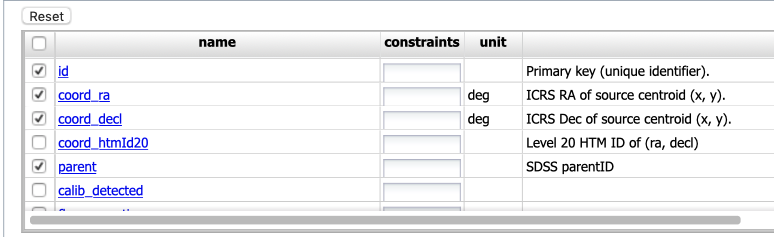
\includegraphics[width=3.12500in]{jira_imgs/244.png}\\

\vspace{\dp0}
} \end{minipage} \\ \cdashline{2-3}
& {\small Test Data} &
\\ \cdashline{2-3}
& {\small Expected Result} &
\begin{minipage}[t]{13cm}{\scriptsize
The column box should be configured to return a minimal useful set of
columns.

\vspace{\dp0}
} \end{minipage}
\\ \hdashline
        \\ \midrule
            \multirow{3}{*}{\parbox{1.3cm}{ 2
} }
& {\small Description} &
\begin{minipage}[t]{13cm}{\scriptsize
Enter an object name for the portal to resolve. ~We will use NGC 359, a
large elliptical galaxy in the Stripe 82 coverage.\\[2\baselineskip]To
do this, enter the name ``NGC 359'' in the ``Name or Position'' text
input box.\\[2\baselineskip]Leave the other defaults in
place.\\[2\baselineskip]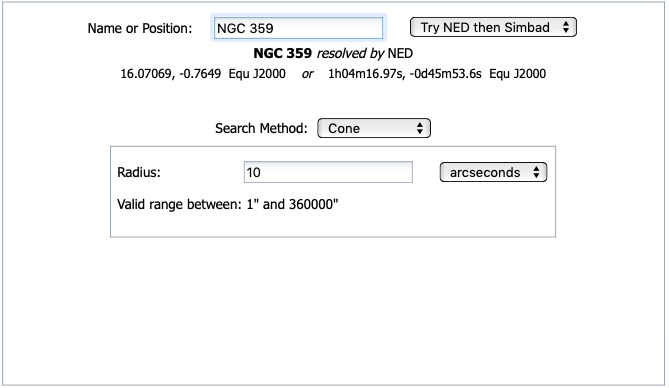
\includegraphics[width=3.12500in]{jira_imgs/245.png}

\vspace{\dp0}
} \end{minipage} \\ \cdashline{2-3}
& {\small Test Data} &
\\ \cdashline{2-3}
& {\small Expected Result} &
\begin{minipage}[t]{13cm}{\scriptsize
There should be a message like ``NGC 359 resolved by NED''. ~The example
coordinates should also changed to the coordinates of NGC 359.

\vspace{\dp0}
} \end{minipage}
\\ \hdashline
        \\ \midrule
            \multirow{3}{*}{\parbox{1.3cm}{ 3
} }
& {\small Description} &
\begin{minipage}[t]{13cm}{\scriptsize
Submit the query to the portal query engine by clicking the ``Search''
button in the lower left corner of the interface.

\vspace{\dp0}
} \end{minipage} \\ \cdashline{2-3}
& {\small Test Data} &
\\ \cdashline{2-3}
& {\small Expected Result} &
\begin{minipage}[t]{13cm}{\scriptsize
A firefly app with the summary image overlay and catalog widgets side by
side. ~A plot of RA vs. Dec is displayed below the side by side
widgets.\\[2\baselineskip]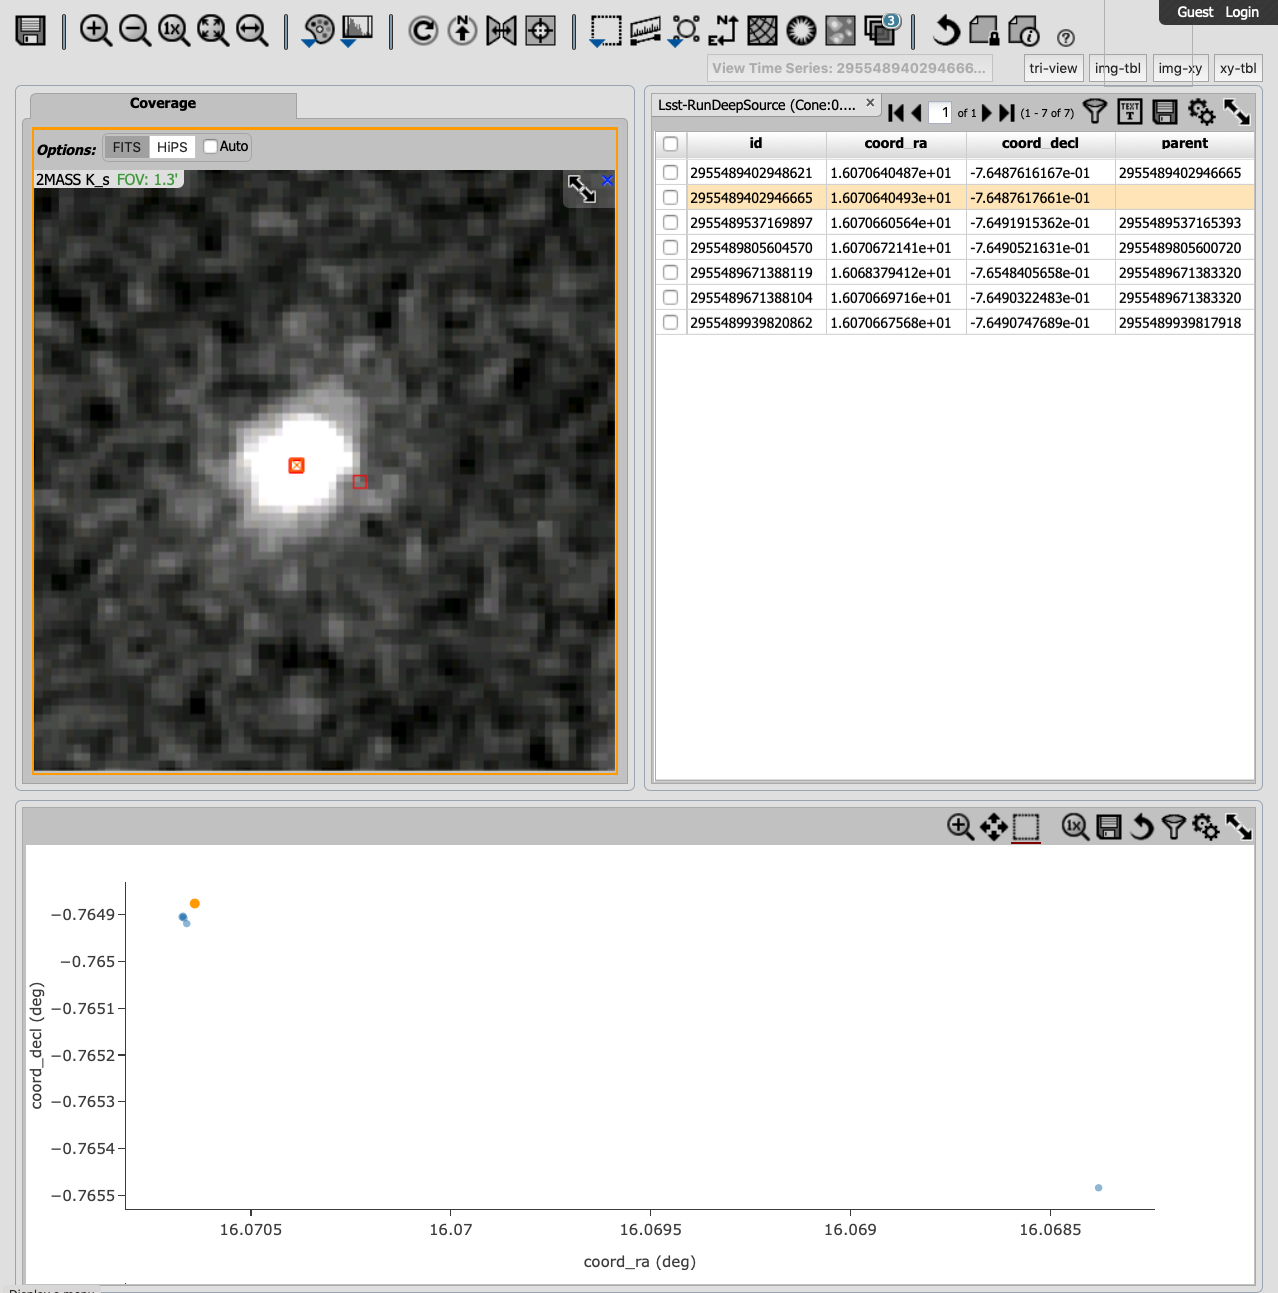
\includegraphics[width=3.12500in]{jira_imgs/246.png}

\vspace{\dp0}
} \end{minipage}
\\ \hdashline
        \\ \midrule
    \end{longtable}


\subsection{LVV-T1591 - Obtain an access token for the TAP service in an LSP instance}\label{lvv-t1591}

\begin{longtable}[]{llllll}
\toprule
Version & Status & Priority & Verification Type & Owner
\\\midrule
1 & Draft & Normal &
Test & Gregory Dubois-Felsmann
\\\bottomrule
\multicolumn{6}{c}{ Open \href{https://jira.lsstcorp.org/secure/Tests.jspa\#/testCase/LVV-T1591}{LVV-T1591} in Jira } \\
\end{longtable}

\subsubsection{Test Items}
Obtain an access token for the TAP service in an LSP instance, enabling
subsequent test steps to connect to the TAP service as an authorized
user.



\subsubsection{Environment Needs}

\paragraph{Software}
An up-to-date Web browser


\subsubsection{Input Specification}
The tester must have credentials for LSP access. ~Either NCSA or
federated non-project credentials may be used.


\subsubsection{Test Procedure}
    \begin{longtable}[]{p{1.3cm}p{2cm}p{13cm}}
    %\toprule
    Step & \multicolumn{2}{@{}l}{Description, Input Data and Expected Result} \\ \toprule
    \endhead
            \multirow{3}{*}{\parbox{1.3cm}{ 1
} }
& {\small Description} &
\begin{minipage}[t]{13cm}{\scriptsize
Using a Web browser, navigate to the\\
``/auth/tokens'' endpoint of the LSP instance under test.

\vspace{\dp0}
} \end{minipage} \\ \cdashline{2-3}
& {\small Test Data} &
\\ \cdashline{2-3}
& {\small Expected Result} &
\begin{minipage}[t]{13cm}{\scriptsize
A credential-entry screen should be displayed, unless the test user is
already logged in in another window or tab of the browser.

\vspace{\dp0}
} \end{minipage}
\\ \hdashline
        \\ \midrule
            \multirow{3}{*}{\parbox{1.3cm}{ 2
} }
& {\small Description} &
\begin{minipage}[t]{13cm}{\scriptsize
If necessary, enter a valid set of credentials. ~They may be NCSA or
non-NCSA credentials.

\vspace{\dp0}
} \end{minipage} \\ \cdashline{2-3}
& {\small Test Data} &
\\ \cdashline{2-3}
& {\small Expected Result} &
\begin{minipage}[t]{13cm}{\scriptsize
The token-request UI is displayed.

\vspace{\dp0}
} \end{minipage}
\\ \hdashline
        \\ \midrule
            \multirow{3}{*}{\parbox{1.3cm}{ 3
} }
& {\small Description} &
\begin{minipage}[t]{13cm}{\scriptsize
Request a token for the ``read:tap'' capability.

\vspace{\dp0}
} \end{minipage} \\ \cdashline{2-3}
& {\small Test Data} &
\\ \cdashline{2-3}
& {\small Expected Result} &
\begin{minipage}[t]{13cm}{\scriptsize
A screen confirming the creation of the token.

\vspace{\dp0}
} \end{minipage}
\\ \hdashline
        \\ \midrule
            \multirow{3}{*}{\parbox{1.3cm}{ 4
} }
& {\small Description} &
\begin{minipage}[t]{13cm}{\scriptsize
Leave the resulting page's browser tab/window open for use in subsequent
test steps.\\[2\baselineskip]In many cases you may be asked in a
subsequent step to use the ``copy token to clipboard'' UI element on
this page in order to transfer your token to a prompt in another window.

\vspace{\dp0}
} \end{minipage} \\ \cdashline{2-3}
& {\small Test Data} &
\\ \cdashline{2-3}
& {\small Expected Result} &
\\ \hdashline
        \\ \midrule
    \end{longtable}





\newpage
\section{Deprecated Test Cases}

This section includes all test cases that have been marked as deprecated.
These test cases will never be executed again, but have been in the past.
For this reason it is important to keep them in the baseline as a reference.



\subsection{LVV-T2 - LSP-00-00: Verification of the presence of the expected WISE data}\label{lvv-t2}

\begin{longtable}[]{llllll}
\toprule
Version & Status & Priority & Verification Type & Owner
\\\midrule
1 & Deprecated & Normal &
Test & Gregory Dubois-Felsmann
\\\bottomrule
\multicolumn{6}{c}{ Open \href{https://jira.lsstcorp.org/secure/Tests.jspa\#/testCase/LVV-T2}{LVV-T2} in Jira } \\
\end{longtable}

\subsubsection{Verification Elements}
\begin{itemize}
\item \href{https://jira.lsstcorp.org/browse/LVV-9807}{LVV-9807} - DMS-LSP-REQ-0001-V-01: Access to All Released or Authorized Data
Products\_1

\item \href{https://jira.lsstcorp.org/browse/LVV-9809}{LVV-9809} - DMS-LSP-REQ-0005-V-01: Linkage of Aspects\_1

\end{itemize}

\subsubsection{Test Items}
This test will check:

\begin{itemize}
\tightlist
\item
  That the expected tables are present in the database and accessible
  via the API Aspect and the Portal Aspect;
\item
  That the tables are present with the expected schema as documented in
  the IPAC- provided WISE documentation;
\item
  That the row counts in the tables are as expected;
\item
  That the tables cover essentially the entire sky, as expected from the
  characteristics of the WISE mission.
\end{itemize}

\textbf{Requirements (to be removed when Reqs are synchronized from
magic draw)}

\begin{itemize}
\tightlist
\item
  DMS-LSP-REQ-0001
\item
  DMS-LSP-REQ-0005
\end{itemize}



\subsection{LVV-T3 - LSP-00-05: Demonstration of low-volume and/or indexed queries against
the WISE data via API}\label{lvv-t3}

\begin{longtable}[]{llllll}
\toprule
Version & Status & Priority & Verification Type & Owner
\\\midrule
1 & Deprecated & Normal &
Test & Gregory Dubois-Felsmann
\\\bottomrule
\multicolumn{6}{c}{ Open \href{https://jira.lsstcorp.org/secure/Tests.jspa\#/testCase/LVV-T3}{LVV-T3} in Jira } \\
\end{longtable}

\subsubsection{Verification Elements}
\begin{itemize}
\item \href{https://jira.lsstcorp.org/browse/LVV-9808}{LVV-9808} - DMS-LSP-REQ-0004-V-01: API (Data Access) Aspect\_1

\end{itemize}

\subsubsection{Test Items}
This test will check that the following low-volume queries can be
performed against the WISE catalogs via the API Aspect.

\begin{itemize}
\tightlist
\item
  Small cone searches against the Object-like, ForcedSource-like, and
  Source-like tables; and
\item
  Searches by exact ID matching against the Object-like,
  ForcedSource-like, and Source- like tables
\end{itemize}

~\\
The tests will record their performance for comparison against similar
queries in the produc- tion WISE archive at IRSA, and the returned data
will be compared to that for similar queries against the API services
provided by IRSA.\\[2\baselineskip]\textbf{Requirement (to remove once
requirements are synchronized from magic draw)}\\
DMS-LSP-REQ-004



\subsection{LVV-T4 - LSP-00-10: Demonstration of table-scan queries against the WISE data via
API}\label{lvv-t4}

\begin{longtable}[]{llllll}
\toprule
Version & Status & Priority & Verification Type & Owner
\\\midrule
1 & Deprecated & Normal &
Test & Gregory Dubois-Felsmann
\\\bottomrule
\multicolumn{6}{c}{ Open \href{https://jira.lsstcorp.org/secure/Tests.jspa\#/testCase/LVV-T4}{LVV-T4} in Jira } \\
\end{longtable}

\subsubsection{Verification Elements}
\begin{itemize}
\item \href{https://jira.lsstcorp.org/browse/LVV-9824}{LVV-9824} - DMS-LSP-REQ-0028-V-01: Peak Volume for Moderate-Sized Queries\_1

\item \href{https://jira.lsstcorp.org/browse/LVV-9825}{LVV-9825} - DMS-LSP-REQ-0029-V-01: Peak Volume for Queries on all Objects\_1

\end{itemize}

\subsubsection{Test Items}
This test exercises a range of table-scan-type queries against the WISE
data. Queries shall be performed against the Object-like table, the
Forced-Source-like table, and against at least one of the Source-like
tables. A range of query result sizes should be exercised, and shall
include at least:

\begin{itemize}
\tightlist
\item
  Queries returning a very small amount of data, fewer than 100 rows,
  and a small subset of columns;
\item
  Queries matching a scaled version of the ``low volume'' query
  definition from the Data Access White Paper; and
\item
  Queries matching a scaled version of the ``high volume'' query
  definition from the Data Access White Paper.
\end{itemize}

The scaling of the ``low volume'' query definition (``50 simultaneous
queries against 10 million objects in the catalog, response 10 sec,
result data set: 0.1 GB'') is based on a assumption that the ``against
10 million objects'' is applied against the O(20 billion) rows
anticipated in the Object table, and that it contemplates reducing the
scope of any non-indexed portion of the WHERE clause of the query to
that fraction of one in ∼ 2000 of the rows in the table. Scaled to the ∼
750 million rows in the WISE Object-like (AllWISE ``Source Catalog'')
table, this would be ∼ 375,000 rows. Similarly scaling the result set
size suggests a result set of ∼ 3.7 MB.\\
Successful completion will be evaluated based on the system's ability to
perform the query at all and to return a result with characteristics
corresponding to plausible estimates or extrap- olations from
scaled-down queries against the IRSA WISE archive. Exact verification
may not be realistic because of the lack of a system capable of
performing the equivalent queries in the production WISE archive.\\
At a later date it may be possible to attempt equivalent queries using a
non-database sys- tem and verify the exact correspondence of results,
but the non-database system does not presently
exist1.\\[3\baselineskip]\textbf{Requirements (to be removed when Reqs
are synchronized from magic draw)}

\begin{itemize}
\tightlist
\item
  DMS-LSP-REQ-0028~
\item
  DMS-LSP-REQ-0029
\end{itemize}



\subsection{LVV-T5 - LSP-00-15: Execution of basic catalog queries in the Portal}\label{lvv-t5}

\begin{longtable}[]{llllll}
\toprule
Version & Status & Priority & Verification Type & Owner
\\\midrule
1 & Deprecated & Normal &
Test & Gregory Dubois-Felsmann
\\\bottomrule
\multicolumn{6}{c}{ Open \href{https://jira.lsstcorp.org/secure/Tests.jspa\#/testCase/LVV-T5}{LVV-T5} in Jira } \\
\end{longtable}

\subsubsection{Verification Elements}
\begin{itemize}
\item \href{https://jira.lsstcorp.org/browse/LVV-9811}{LVV-9811} - DMS-LSP-REQ-0002-V-01: Portal Aspect\_1

\item \href{https://jira.lsstcorp.org/browse/LVV-9819}{LVV-9819} - DMS-LSP-REQ-0014-V-01: Download Data\_1

\item \href{https://jira.lsstcorp.org/browse/LVV-9862}{LVV-9862} - DMS-PRTL-REQ-0022-V-01: Positional Query: Astrophysical Coordinate
Systems\_1

\item \href{https://jira.lsstcorp.org/browse/LVV-9865}{LVV-9865} - DMS-PRTL-REQ-0021-V-01: Positional Query: Multiple Positions/Objects\_1

\item \href{https://jira.lsstcorp.org/browse/LVV-9869}{LVV-9869} - DMS-PRTL-REQ-0026-V-01: Positional Query by Region: Cone-Search\_1

\item \href{https://jira.lsstcorp.org/browse/LVV-9868}{LVV-9868} - DMS-PRTL-REQ-0027-V-01: Positional Query by Region: Box-Search\_1

\item \href{https://jira.lsstcorp.org/browse/LVV-9859}{LVV-9859} - DMS-PRTL-REQ-0028-V-01: Query by Identifier\_1

\item \href{https://jira.lsstcorp.org/browse/LVV-9856}{LVV-9856} - DMS-PRTL-REQ-0016-V-01: Generic Query - Form-based\_1

\end{itemize}

\subsubsection{Test Items}
This test will test the functional requirements to be able to perform a
range of basic queries through the Portal Aspect of the LSP:

\begin{itemize}
\tightlist
\item
  Cone searches on the Object-like, ForcedSource-like, and Source-like
  WISE tables;~
\item
  Multi-target cone searches;
\item
  Form-based searches for exact equality, e.g., for row IDs; and
\item
  Form-based searches for sets of object attributes.
\end{itemize}

In addition, it tests the ability to download tabular query results from
the Portal Aspect.



\subsection{LVV-T6 - LSP-00-20: Operation of the UI for interaction with tabular data results}\label{lvv-t6}

\begin{longtable}[]{llllll}
\toprule
Version & Status & Priority & Verification Type & Owner
\\\midrule
1 & Deprecated & Normal &
Test & Gregory Dubois-Felsmann
\\\bottomrule
\multicolumn{6}{c}{ Open \href{https://jira.lsstcorp.org/secure/Tests.jspa\#/testCase/LVV-T6}{LVV-T6} in Jira } \\
\end{longtable}

\subsubsection{Verification Elements}
\begin{itemize}
\item \href{https://jira.lsstcorp.org/browse/LVV-9895}{LVV-9895} - DMS-PRTL-REQ-0056-V-01: Histograms\_1

\item \href{https://jira.lsstcorp.org/browse/LVV-9901}{LVV-9901} - DMS-PRTL-REQ-0055-V-01: XY Scatter Plots\_1

\item \href{https://jira.lsstcorp.org/browse/LVV-9893}{LVV-9893} - DMS-PRTL-REQ-0054-V-01: Paging of Tabular Data\_1

\item \href{https://jira.lsstcorp.org/browse/LVV-9889}{LVV-9889} - DMS-PRTL-REQ-0050-V-01: Column Selection of Tabular Data\_1

\item \href{https://jira.lsstcorp.org/browse/LVV-9894}{LVV-9894} - DMS-PRTL-REQ-0053-V-01: Row Selection of Tabular Data\_1

\item \href{https://jira.lsstcorp.org/browse/LVV-9891}{LVV-9891} - DMS-PRTL-REQ-0049-V-01: Display of Tabular Data\_1

\item \href{https://jira.lsstcorp.org/browse/LVV-9819}{LVV-9819} - DMS-LSP-REQ-0014-V-01: Download Data\_1

\item \href{https://jira.lsstcorp.org/browse/LVV-9821}{LVV-9821} - DMS-LSP-REQ-0017-V-01: Tabular Data Download File Formats\_1

\end{itemize}

\subsubsection{Test Items}
This test will test the functional requirements to be able to perform
certain basic exploratory data analysis functions on tabular data
results in the Portal Aspect UI:

\begin{itemize}
\tightlist
\item
  Sort tabular results;
\item
  Filter tabular results based on the contents of columns;~
\item
  Perform per-row selections from a table;
\item
  Display 1D histograms of selected attributes;
\item
  Display 2D scatter plots of selected attributes;
\item
  Perform graphical selections of rows from plots; and
\item
  Download tabular query results reflecting sorting and selection.
\end{itemize}

This test does not address the limits of scaling of these capabilities
to large query results. That will be addressed in future test
specifications. The test report should include notes on the sizes of
results that were used.



\subsection{LVV-T7 - LSP-00-25: Image metadata, image, and image cutout queries}\label{lvv-t7}

\begin{longtable}[]{llllll}
\toprule
Version & Status & Priority & Verification Type & Owner
\\\midrule
1 & Deprecated & Normal &
Test & Gregory Dubois-Felsmann
\\\bottomrule
\multicolumn{6}{c}{ Open \href{https://jira.lsstcorp.org/secure/Tests.jspa\#/testCase/LVV-T7}{LVV-T7} in Jira } \\
\end{longtable}

\subsubsection{Verification Elements}
\begin{itemize}
\item \href{https://jira.lsstcorp.org/browse/LVV-9819}{LVV-9819} - DMS-LSP-REQ-0014-V-01: Download Data\_1

\item \href{https://jira.lsstcorp.org/browse/LVV-9820}{LVV-9820} - DMS-LSP-REQ-0018-V-01: Image Data Download File Format\_1

\item \href{https://jira.lsstcorp.org/browse/LVV-9881}{LVV-9881} - DMS-PRTL-REQ-0040-V-01: Query for Single Epoch Image Cutouts\_1

\item \href{https://jira.lsstcorp.org/browse/LVV-9880}{LVV-9880} - DMS-PRTL-REQ-0041-V-01: Query for Coadded Image Cutouts\_1

\end{itemize}

\subsubsection{Test Items}
This test will check basic functionality related to image search and
retrieval, via both the API Aspect and the Portal Aspect of the LSST
Science Platform:

\begin{itemize}
\tightlist
\item
  Searching for images containing a specified point;
\item
  Displaying selected images;
\item
  Obtaining and displaying image cutouts at a specified point; and
\item
  Downloading selected images and image cutouts.
\end{itemize}

Because of limited staff resources, these tests will be based on the
original PDAC dataset, the LSST Summer 2013 processing of the SDSS
Stripe 82 data. The image data for the WISE and NEOWISE missions have
not been loaded into PDAC.\\[2\baselineskip]



\subsection{LVV-T8 - LSP-00-30: Linkage of catalog query results with associated images}\label{lvv-t8}

\begin{longtable}[]{llllll}
\toprule
Version & Status & Priority & Verification Type & Owner
\\\midrule
1 & Deprecated & Normal &
Test & Gregory Dubois-Felsmann
\\\bottomrule
\multicolumn{6}{c}{ Open \href{https://jira.lsstcorp.org/secure/Tests.jspa\#/testCase/LVV-T8}{LVV-T8} in Jira } \\
\end{longtable}

\subsubsection{Verification Elements}
\begin{itemize}
\item \href{https://jira.lsstcorp.org/browse/LVV-9848}{LVV-9848} - DMS-PRTL-REQ-0004-V-01: Semantic Linkage: Portal Workflows\_1

\item \href{https://jira.lsstcorp.org/browse/LVV-9814}{LVV-9814} - DMS-LSP-REQ-0008-V-01: Semantic Linkage\_1

\end{itemize}

\subsubsection{Test Items}
This test will check for the ability, in the Portal Aspect of the LSST
Science Platform, to match catalog data with the image data on which the
measurements were performed, specifically:

\begin{itemize}
\tightlist
\item
  Navigating from a catalog query result to the associated images; and~
\item
  Overlaying catalog query results on associated images.
\end{itemize}

Because of limited staff resources, these tests will be based on the
original PDAC dataset, the LSST Summer 2013 processing of the SDSS
Stripe 82 data. The image data for the WISE and NEOWISE missions have
not been loaded into PDAC.



\subsection{LVV-T9 - LSP-00-35: Linkage of catalog query results to related catalog data}\label{lvv-t9}

\begin{longtable}[]{llllll}
\toprule
Version & Status & Priority & Verification Type & Owner
\\\midrule
1 & Deprecated & Normal &
Test & Gregory Dubois-Felsmann
\\\bottomrule
\multicolumn{6}{c}{ Open \href{https://jira.lsstcorp.org/secure/Tests.jspa\#/testCase/LVV-T9}{LVV-T9} in Jira } \\
\end{longtable}

\subsubsection{Verification Elements}
\begin{itemize}
\item \href{https://jira.lsstcorp.org/browse/LVV-9814}{LVV-9814} - DMS-LSP-REQ-0008-V-01: Semantic Linkage\_1

\end{itemize}

\subsubsection{Test Items}
This test will check for the ability, in the Portal Aspect of the LSST
Science Platform, to match catalog data with related catalog data.
Specifically, the test verifies the ability to navigate from a coadded
source catalog entry to the associated forced
photometry.\\[2\baselineskip]\textbf{Requirements (to be removed when
Reqs are synchronized from magic draw)}

\begin{itemize}
\tightlist
\item
  DMS-LSP-REQ-0008
\end{itemize}




\newpage
\appendix
